\documentclass[twoside]{book}

% Packages required by doxygen
\usepackage{fixltx2e}
\usepackage{calc}
\usepackage{doxygen}
\usepackage[export]{adjustbox} % also loads graphicx
\usepackage{graphicx}
\usepackage[utf8]{inputenc}
\usepackage{makeidx}
\usepackage{multicol}
\usepackage{multirow}
\PassOptionsToPackage{warn}{textcomp}
\usepackage{textcomp}
\usepackage[nointegrals]{wasysym}
\usepackage[table]{xcolor}

% Font selection
\usepackage[T1]{fontenc}
\usepackage[scaled=.90]{helvet}
\usepackage{courier}
\usepackage{amssymb}
\usepackage{sectsty}
\renewcommand{\familydefault}{\sfdefault}
\allsectionsfont{%
  \fontseries{bc}\selectfont%
  \color{darkgray}%
}
\renewcommand{\DoxyLabelFont}{%
  \fontseries{bc}\selectfont%
  \color{darkgray}%
}
\newcommand{\+}{\discretionary{\mbox{\scriptsize$\hookleftarrow$}}{}{}}

% Page & text layout
\usepackage{geometry}
\geometry{%
  a4paper,%
  top=2.5cm,%
  bottom=2.5cm,%
  left=2.5cm,%
  right=2.5cm%
}
\tolerance=750
\hfuzz=15pt
\hbadness=750
\setlength{\emergencystretch}{15pt}
\setlength{\parindent}{0cm}
\setlength{\parskip}{0.2cm}
\makeatletter
\renewcommand{\paragraph}{%
  \@startsection{paragraph}{4}{0ex}{-1.0ex}{1.0ex}{%
    \normalfont\normalsize\bfseries\SS@parafont%
  }%
}
\renewcommand{\subparagraph}{%
  \@startsection{subparagraph}{5}{0ex}{-1.0ex}{1.0ex}{%
    \normalfont\normalsize\bfseries\SS@subparafont%
  }%
}
\makeatother

% Headers & footers
\usepackage{fancyhdr}
\pagestyle{fancyplain}
\fancyhead[LE]{\fancyplain{}{\bfseries\thepage}}
\fancyhead[CE]{\fancyplain{}{}}
\fancyhead[RE]{\fancyplain{}{\bfseries\leftmark}}
\fancyhead[LO]{\fancyplain{}{\bfseries\rightmark}}
\fancyhead[CO]{\fancyplain{}{}}
\fancyhead[RO]{\fancyplain{}{\bfseries\thepage}}
\fancyfoot[LE]{\fancyplain{}{}}
\fancyfoot[CE]{\fancyplain{}{}}
\fancyfoot[RE]{\fancyplain{}{\bfseries\scriptsize Generated on Sat Jun 25 2016 01\+:54\+:45 for My Project by Doxygen }}
\fancyfoot[LO]{\fancyplain{}{\bfseries\scriptsize Generated on Sat Jun 25 2016 01\+:54\+:45 for My Project by Doxygen }}
\fancyfoot[CO]{\fancyplain{}{}}
\fancyfoot[RO]{\fancyplain{}{}}
\renewcommand{\footrulewidth}{0.4pt}
\renewcommand{\chaptermark}[1]{%
  \markboth{#1}{}%
}
\renewcommand{\sectionmark}[1]{%
  \markright{\thesection\ #1}%
}

% Indices & bibliography
\usepackage{natbib}
\usepackage[titles]{tocloft}
\setcounter{tocdepth}{3}
\setcounter{secnumdepth}{5}
\makeindex

% Hyperlinks (required, but should be loaded last)
\usepackage{ifpdf}
\ifpdf
  \usepackage[pdftex,pagebackref=true]{hyperref}
\else
  \usepackage[ps2pdf,pagebackref=true]{hyperref}
\fi
\hypersetup{%
  colorlinks=true,%
  linkcolor=blue,%
  citecolor=blue,%
  unicode%
}

% Custom commands
\newcommand{\clearemptydoublepage}{%
  \newpage{\pagestyle{empty}\cleardoublepage}%
}


%===== C O N T E N T S =====

\begin{document}

% Titlepage & ToC
\hypersetup{pageanchor=false,
             bookmarks=true,
             bookmarksnumbered=true,
             pdfencoding=unicode
            }
\pagenumbering{roman}
\begin{titlepage}
\vspace*{7cm}
\begin{center}%
{\Large My Project \\[1ex]\large 0.\+5 }\\
\vspace*{1cm}
{\large Generated by Doxygen 1.8.10}\\
\vspace*{0.5cm}
{\small Sat Jun 25 2016 01:54:45}\\
\end{center}
\end{titlepage}
\clearemptydoublepage
\tableofcontents
\clearemptydoublepage
\pagenumbering{arabic}
\hypersetup{pageanchor=true}

%--- Begin generated contents ---
\chapter{Namespace Index}
\section{Packages}
Here are the packages with brief descriptions (if available)\+:\begin{DoxyCompactList}
\item\contentsline{section}{\hyperlink{namespace_graph_library}{Graph\+Library} \\*Defines 5 things\+: 1) Port Mode Enumeration \+: Its an enumeration that describes the node port direction It has 3 distinct values S\+O\+U\+R\+C\+E, T\+A\+R\+G\+E\+T (directed graphs ) and T\+W\+O\+W\+A\+Y (undirected graphs ) 2) \hyperlink{class_graph_library_1_1_c_graph_node}{C\+Graph\+Node} class \+: The base class for graph node modelling. 3) C\+Node\+Port class \+: The base class for port modelling 4) \hyperlink{class_graph_library_1_1_c_graph_edge}{C\+Graph\+Edge} \+: The base class for edge modelling 5) \hyperlink{class_graph_library_1_1_c_graph}{C\+Graph} \+: The base class for graph modelling }{\pageref{namespace_graph_library}}{}
\item\contentsline{section}{\hyperlink{namespace_graph_library_1_1_aglorithms}{Graph\+Library.\+Aglorithms} }{\pageref{namespace_graph_library_1_1_aglorithms}}{}
\item\contentsline{section}{\hyperlink{namespace_graph_library_1_1_generics}{Graph\+Library.\+Generics} }{\pageref{namespace_graph_library_1_1_generics}}{}
\item\contentsline{section}{\hyperlink{namespace_graph_library_1_1_printers}{Graph\+Library.\+Printers} }{\pageref{namespace_graph_library_1_1_printers}}{}
\item\contentsline{section}{\hyperlink{namespace_graph_library_1_1_printers_1_1_graph_viz_printer}{Graph\+Library.\+Printers.\+Graph\+Viz\+Printer} }{\pageref{namespace_graph_library_1_1_printers_1_1_graph_viz_printer}}{}
\end{DoxyCompactList}

\chapter{Hierarchical Index}
\section{Class Hierarchy}
This inheritance list is sorted roughly, but not completely, alphabetically\+:\begin{DoxyCompactList}
\item \contentsline{section}{Graph\+Library.\+Generics.\+Abstract\+Graph\+Algorithm$<$ T, C\+Graph\+Node, C\+Graph\+Edge, C\+Graph $>$}{\pageref{class_graph_library_1_1_generics_1_1_abstract_graph_algorithm}}{}
\begin{DoxyCompactList}
\item \contentsline{section}{Graph\+Library.\+C\+Graph\+Algorithm$<$ T $>$}{\pageref{class_graph_library_1_1_c_graph_algorithm}}{}
\end{DoxyCompactList}
\item \contentsline{section}{Graph\+Library.\+Generics.\+Abstract\+Graph\+Iterator$<$ C\+Graph\+Edge $>$}{\pageref{class_graph_library_1_1_generics_1_1_abstract_graph_iterator}}{}
\begin{DoxyCompactList}
\item \contentsline{section}{Graph\+Library.\+C\+It\+\_\+\+Graph\+Edges}{\pageref{class_graph_library_1_1_c_it___graph_edges}}{}
\end{DoxyCompactList}
\item \contentsline{section}{Graph\+Library.\+Generics.\+Abstract\+Graph\+Iterator$<$ C\+Graph\+Node $>$}{\pageref{class_graph_library_1_1_generics_1_1_abstract_graph_iterator}}{}
\begin{DoxyCompactList}
\item \contentsline{section}{Graph\+Library.\+C\+It\+\_\+\+Graph\+B\+F\+S}{\pageref{class_graph_library_1_1_c_it___graph_b_f_s}}{}
\item \contentsline{section}{Graph\+Library.\+C\+It\+\_\+\+Graph\+D\+F\+S}{\pageref{class_graph_library_1_1_c_it___graph_d_f_s}}{}
\item \contentsline{section}{Graph\+Library.\+C\+It\+\_\+\+Graph\+Leaf\+Nodes}{\pageref{class_graph_library_1_1_c_it___graph_leaf_nodes}}{}
\item \contentsline{section}{Graph\+Library.\+C\+It\+\_\+\+Graph\+Nodes}{\pageref{class_graph_library_1_1_c_it___graph_nodes}}{}
\item \contentsline{section}{Graph\+Library.\+C\+It\+\_\+\+Graph\+Root\+Nodes}{\pageref{class_graph_library_1_1_c_it___graph_root_nodes}}{}
\item \contentsline{section}{Graph\+Library.\+C\+It\+\_\+\+Predecessors}{\pageref{class_graph_library_1_1_c_it___predecessors}}{}
\item \contentsline{section}{Graph\+Library.\+C\+It\+\_\+\+Successors}{\pageref{class_graph_library_1_1_c_it___successors}}{}
\end{DoxyCompactList}
\item \contentsline{section}{Graph\+Library.\+Generics.\+Abstract\+Graph\+Iterator\+Factory$<$ T\+Node, T\+Edge, T\+Graph $>$}{\pageref{class_graph_library_1_1_generics_1_1_abstract_graph_iterator_factory}}{}
\item \contentsline{section}{Graph\+Library.\+Generics.\+Abstract\+Graph\+Iterator\+Factory$<$ C\+Graph\+Node, C\+Graph\+Edge, C\+Graph $>$}{\pageref{class_graph_library_1_1_generics_1_1_abstract_graph_iterator_factory}}{}
\begin{DoxyCompactList}
\item \contentsline{section}{Graph\+Library.\+C\+Graph\+Iterators\+Factory}{\pageref{class_graph_library_1_1_c_graph_iterators_factory}}{}
\end{DoxyCompactList}
\item \contentsline{section}{Graph\+Library.\+Generics.\+Abstract\+Graph\+Labeling$<$ T $>$}{\pageref{class_graph_library_1_1_generics_1_1_abstract_graph_labeling}}{}
\begin{DoxyCompactList}
\item \contentsline{section}{Graph\+Library.\+C\+Graph\+Labeling$<$ T $>$}{\pageref{class_graph_library_1_1_c_graph_labeling}}{}
\end{DoxyCompactList}
\item \contentsline{section}{Graph\+Library.\+Generics.\+Abstract\+Graph\+Printer$<$ T\+Graph $>$}{\pageref{class_graph_library_1_1_generics_1_1_abstract_graph_printer}}{}
\item \contentsline{section}{Graph\+Library.\+Generics.\+Abstract\+Graph\+Printer$<$ C\+Graph $>$}{\pageref{class_graph_library_1_1_generics_1_1_abstract_graph_printer}}{}
\begin{DoxyCompactList}
\item \contentsline{section}{Graph\+Library.\+C\+Graph\+Printer}{\pageref{class_graph_library_1_1_c_graph_printer}}{}
\begin{DoxyCompactList}
\item \contentsline{section}{Graph\+Library.\+C\+Graph\+Viz\+Printer}{\pageref{class_graph_library_1_1_c_graph_viz_printer}}{}
\end{DoxyCompactList}
\end{DoxyCompactList}
\item \contentsline{section}{Graph\+Library.\+Generics.\+Abstract\+Graph\+Query\+Info$<$ Node, Edge, Graph $>$}{\pageref{class_graph_library_1_1_generics_1_1_abstract_graph_query_info}}{}
\item \contentsline{section}{Graph\+Library.\+Generics.\+Abstract\+Graph\+Query\+Info$<$ C\+Graph\+Node, C\+Graph\+Edge, C\+Graph $>$}{\pageref{class_graph_library_1_1_generics_1_1_abstract_graph_query_info}}{}
\begin{DoxyCompactList}
\item \contentsline{section}{Graph\+Library.\+C\+Graph\+Query\+Info}{\pageref{class_graph_library_1_1_c_graph_query_info}}{}
\end{DoxyCompactList}
\item \contentsline{section}{Graph\+Library.\+Generics.\+Abstract\+Graph\+Query\+Info$<$ T\+Node, T\+Edge, T\+Graph $>$}{\pageref{class_graph_library_1_1_generics_1_1_abstract_graph_query_info}}{}
\item \contentsline{section}{Graph\+Library.\+C\+Graph\+Algorithm$<$ C\+Graph\+Edge $>$}{\pageref{class_graph_library_1_1_c_graph_algorithm}}{}
\begin{DoxyCompactList}
\item \contentsline{section}{Graph\+Library.\+Aglorithms.\+G\+Alg\+\_\+\+Edge\+Oriented\+D\+F\+S}{\pageref{class_graph_library_1_1_aglorithms_1_1_g_alg___edge_oriented_d_f_s}}{}
\end{DoxyCompactList}
\item \contentsline{section}{Graph\+Library.\+C\+Graph\+Algorithm$<$ C\+Graph\+Node $>$}{\pageref{class_graph_library_1_1_c_graph_algorithm}}{}
\begin{DoxyCompactList}
\item \contentsline{section}{Graph\+Library.\+Aglorithms.\+G\+Alg\+\_\+\+Node\+Oriented\+D\+F\+S}{\pageref{class_graph_library_1_1_aglorithms_1_1_g_alg___node_oriented_d_f_s}}{}
\end{DoxyCompactList}
\item \contentsline{section}{Graph\+Library.\+C\+Graph\+Labeling$<$ C\+Graph\+Node $>$}{\pageref{class_graph_library_1_1_c_graph_labeling}}{}
\begin{DoxyCompactList}
\item \contentsline{section}{Graph\+Library.\+Printers.\+Graph\+Viz\+Printer.\+Graph\+Viz\+Node\+Labeling}{\pageref{class_graph_library_1_1_printers_1_1_graph_viz_printer_1_1_graph_viz_node_labeling}}{}
\end{DoxyCompactList}
\item Event\+Args\begin{DoxyCompactList}
\item \contentsline{section}{Graph\+Library.\+Aglorithms.\+Edge\+Info\+\_\+\+D\+F\+S}{\pageref{class_graph_library_1_1_aglorithms_1_1_edge_info___d_f_s}}{}
\item \contentsline{section}{Graph\+Library.\+Aglorithms.\+Node\+Info\+\_\+\+D\+F\+S}{\pageref{class_graph_library_1_1_aglorithms_1_1_node_info___d_f_s}}{}
\end{DoxyCompactList}
\item \contentsline{section}{Graph\+Library.\+Generics.\+I\+Graph\+Algorithm$<$ T, T\+Node $>$}{\pageref{interface_graph_library_1_1_generics_1_1_i_graph_algorithm}}{}
\begin{DoxyCompactList}
\item \contentsline{section}{Graph\+Library.\+Generics.\+Abstract\+Graph\+Algorithm$<$ T, T\+Node, T\+Edge, T\+Graph $>$}{\pageref{class_graph_library_1_1_generics_1_1_abstract_graph_algorithm}}{}
\end{DoxyCompactList}
\item \contentsline{section}{Graph\+Library.\+Generics.\+I\+Graph\+Iterator$<$ T $>$}{\pageref{interface_graph_library_1_1_generics_1_1_i_graph_iterator}}{}
\begin{DoxyCompactList}
\item \contentsline{section}{Graph\+Library.\+Generics.\+Abstract\+Graph\+Iterator$<$ T $>$}{\pageref{class_graph_library_1_1_generics_1_1_abstract_graph_iterator}}{}
\end{DoxyCompactList}
\item \contentsline{section}{Graph\+Library.\+Generics.\+I\+Graph\+Labeling$<$ T $>$}{\pageref{interface_graph_library_1_1_generics_1_1_i_graph_labeling}}{}
\item \contentsline{section}{Graph\+Library.\+Generics.\+I\+Graph\+Labeling$<$ T\+Element $>$}{\pageref{interface_graph_library_1_1_generics_1_1_i_graph_labeling}}{}
\begin{DoxyCompactList}
\item \contentsline{section}{Graph\+Library.\+Generics.\+Abstract\+Graph\+Labeling$<$ T\+Element $>$}{\pageref{class_graph_library_1_1_generics_1_1_abstract_graph_labeling}}{}
\end{DoxyCompactList}
\item \contentsline{section}{Graph\+Library.\+Generics.\+I\+Graph\+Primitive}{\pageref{interface_graph_library_1_1_generics_1_1_i_graph_primitive}}{}
\begin{DoxyCompactList}
\item \contentsline{section}{Graph\+Library.\+C\+Graph\+Edge}{\pageref{class_graph_library_1_1_c_graph_edge}}{}
\item \contentsline{section}{Graph\+Library.\+C\+Graph\+Node}{\pageref{class_graph_library_1_1_c_graph_node}}{}
\begin{DoxyCompactList}
\item \contentsline{section}{Graph\+Library.\+C\+Graph}{\pageref{class_graph_library_1_1_c_graph}}{}
\end{DoxyCompactList}
\end{DoxyCompactList}
\item \contentsline{section}{Graph\+Library.\+C\+It\+\_\+\+Graph\+B\+F\+S.\+Info\+\_\+\+D\+F\+S}{\pageref{class_graph_library_1_1_c_it___graph_b_f_s_1_1_info___d_f_s}}{}
\item \contentsline{section}{Graph\+Library.\+C\+It\+\_\+\+Graph\+D\+F\+S.\+Info\+\_\+\+D\+F\+S}{\pageref{class_graph_library_1_1_c_it___graph_d_f_s_1_1_info___d_f_s}}{}
\end{DoxyCompactList}

\chapter{Class Index}
\section{Class List}
Here are the classes, structs, unions and interfaces with brief descriptions\+:\begin{DoxyCompactList}
\item\contentsline{section}{\hyperlink{class_graph_library_1_1_generics_1_1_abstract_graph_algorithm}{Graph\+Library.\+Generics.\+Abstract\+Graph\+Algorithm$<$ T, T\+Node, T\+Edge, T\+Graph $>$} \\*The abstract base class of the algorithms applied on graphs }{\pageref{class_graph_library_1_1_generics_1_1_abstract_graph_algorithm}}{}
\item\contentsline{section}{\hyperlink{class_graph_library_1_1_generics_1_1_abstract_graph_iterator}{Graph\+Library.\+Generics.\+Abstract\+Graph\+Iterator$<$ T $>$} \\*This class is the base abstract class of Graph\+Iterators. It has no implementation except from the m\+\_\+current\+Item member variable. This variable always point to the current element (which has type T) that the iterator points. The class\textquotesingle{}s methods are executed in a specific sequence that is dictated by the loop statement semantics that is \hyperlink{class_graph_library_1_1_generics_1_1_abstract_graph_iterator_a2c97c7a412c233b8442b7ad403f29779}{Begin()}, \hyperlink{class_graph_library_1_1_generics_1_1_abstract_graph_iterator_aa8cd9f596ec0b6c4c1e9c244ba75df04}{End()}, L\+O\+O\+P\+\_\+\+B\+O\+D\+Y, \hyperlink{class_graph_library_1_1_generics_1_1_abstract_graph_iterator_aac8cffd0d579708a94ba056e4f4a00b2}{Next()}, \hyperlink{class_graph_library_1_1_generics_1_1_abstract_graph_iterator_aa8cd9f596ec0b6c4c1e9c244ba75df04}{End()}, L\+O\+O\+P\+\_\+\+B\+O\+D\+Y, \hyperlink{class_graph_library_1_1_generics_1_1_abstract_graph_iterator_aac8cffd0d579708a94ba056e4f4a00b2}{Next()}, \hyperlink{class_graph_library_1_1_generics_1_1_abstract_graph_iterator_aa8cd9f596ec0b6c4c1e9c244ba75df04}{End()}, L\+O\+O\+P\+\_\+\+B\+O\+D\+Y, \hyperlink{class_graph_library_1_1_generics_1_1_abstract_graph_iterator_aac8cffd0d579708a94ba056e4f4a00b2}{Next()}, \hyperlink{class_graph_library_1_1_generics_1_1_abstract_graph_iterator_aa8cd9f596ec0b6c4c1e9c244ba75df04}{End()}... etc }{\pageref{class_graph_library_1_1_generics_1_1_abstract_graph_iterator}}{}
\item\contentsline{section}{\hyperlink{class_graph_library_1_1_generics_1_1_abstract_graph_iterator_factory}{Graph\+Library.\+Generics.\+Abstract\+Graph\+Iterator\+Factory$<$ T\+Node, T\+Edge, T\+Graph $>$} \\*This class is for programmers convinience. It instanciates iterators that iterate over a graph\textquotesingle{}s elements required for the algorithms and other graph processing facilities }{\pageref{class_graph_library_1_1_generics_1_1_abstract_graph_iterator_factory}}{}
\item\contentsline{section}{\hyperlink{class_graph_library_1_1_generics_1_1_abstract_graph_labeling}{Graph\+Library.\+Generics.\+Abstract\+Graph\+Labeling$<$ T\+Element $>$} \\*This class holds the labels for a specific type of elements (edge , nodes, graphs ) of a graph. I use two dictionaries for both mapping to gain in query speed. This class gives the opportunity that diffrent graph clients can assign diffrent labels to the graph nodes, edges etc. The graph client ( contructor ) creates a subclass of \hyperlink{class_graph_library_1_1_generics_1_1_abstract_graph_labeling}{Abstract\+Graph\+Labeling$<$\+T$>$} and assigns labels to nodes. The instance of this class exists inside the \hyperlink{class_graph_library_1_1_c_graph}{C\+Graph} class and the client can add a new labeling of graph elements through the Add\+Graph\+Node\+Labelling() method. }{\pageref{class_graph_library_1_1_generics_1_1_abstract_graph_labeling}}{}
\item\contentsline{section}{\hyperlink{class_graph_library_1_1_generics_1_1_abstract_graph_printer}{Graph\+Library.\+Generics.\+Abstract\+Graph\+Printer$<$ T\+Graph $>$} \\*This class is the parent class of all classes that print \hyperlink{class_graph_library_1_1_c_graph}{C\+Graph} objects Hence the class know the interface of \hyperlink{class_graph_library_1_1_c_graph}{C\+Graph}. (Its build for \hyperlink{class_graph_library_1_1_c_graph}{C\+Graph}). This class heirarchy is based on the Builder design pattern. }{\pageref{class_graph_library_1_1_generics_1_1_abstract_graph_printer}}{}
\item\contentsline{section}{\hyperlink{class_graph_library_1_1_generics_1_1_abstract_graph_query_info}{Graph\+Library.\+Generics.\+Abstract\+Graph\+Query\+Info$<$ Node, Edge, Graph $>$} \\*The purpose of this class is to simplify the expressions that the designer should write to access graph information from the code that describes the algorithm. This way the code that describes the algorithm is described with minimal complexity expressions something necessery to make him easily readapt to the code after long periods of abstention from this framework The class provides general access (takes object and returns object) to the node/edge information and requires casting to specialize it. }{\pageref{class_graph_library_1_1_generics_1_1_abstract_graph_query_info}}{}
\item\contentsline{section}{\hyperlink{class_graph_library_1_1_c_graph}{Graph\+Library.\+C\+Graph} \\*The Graph holds the list of nodes and the list of edges as well as the type of graph ( directed / undirected ) }{\pageref{class_graph_library_1_1_c_graph}}{}
\item\contentsline{section}{\hyperlink{class_graph_library_1_1_c_graph_algorithm}{Graph\+Library.\+C\+Graph\+Algorithm$<$ T $>$} \\*This is an abstract class that represents algorithms that run on graphs with the following types of elements 1) \hyperlink{class_graph_library_1_1_c_graph_node}{C\+Graph\+Node} for nodes 2) \hyperlink{class_graph_library_1_1_c_graph_edge}{C\+Graph\+Edge} for edges 3) \hyperlink{class_graph_library_1_1_c_graph}{C\+Graph} for graphs }{\pageref{class_graph_library_1_1_c_graph_algorithm}}{}
\item\contentsline{section}{\hyperlink{class_graph_library_1_1_c_graph_edge}{Graph\+Library.\+C\+Graph\+Edge} \\*A graph edges interconnects to Nodes ports that in sequence belong to a node The \hyperlink{class_graph_library_1_1_c_graph_edge}{C\+Graph\+Edge} class stores a reference to the source and target ports. And can provide through properties the source and target ports and nodes. It also provides given the port or node at the one side of the edge the corresponding port or node at the side. }{\pageref{class_graph_library_1_1_c_graph_edge}}{}
\item\contentsline{section}{\hyperlink{class_graph_library_1_1_c_graph_iterators_factory}{Graph\+Library.\+C\+Graph\+Iterators\+Factory} }{\pageref{class_graph_library_1_1_c_graph_iterators_factory}}{}
\item\contentsline{section}{\hyperlink{class_graph_library_1_1_c_graph_labeling}{Graph\+Library.\+C\+Graph\+Labeling$<$ T $>$} \\*This class provides general graph labelling capabilities. It doesn\textquotesingle{}t follow a specific strategy to label nodes/edges. It just implements the default version of Set\+Label methods for the class \hyperlink{class_graph_library_1_1_c_graph}{C\+Graph}. (This class is specific to \hyperlink{class_graph_library_1_1_c_graph}{C\+Graph} class) }{\pageref{class_graph_library_1_1_c_graph_labeling}}{}
\item\contentsline{section}{\hyperlink{class_graph_library_1_1_c_graph_node}{Graph\+Library.\+C\+Graph\+Node} \\*Represents a graph node . }{\pageref{class_graph_library_1_1_c_graph_node}}{}
\item\contentsline{section}{\hyperlink{class_graph_library_1_1_c_graph_printer}{Graph\+Library.\+C\+Graph\+Printer} \\*This class is the parent class of all classes that print \hyperlink{class_graph_library_1_1_c_graph}{C\+Graph} objects Hence the class know the interface of \hyperlink{class_graph_library_1_1_c_graph}{C\+Graph}. (Its build for \hyperlink{class_graph_library_1_1_c_graph}{C\+Graph}). This class heirarchy is based on the Builder design pattern. }{\pageref{class_graph_library_1_1_c_graph_printer}}{}
\item\contentsline{section}{\hyperlink{class_graph_library_1_1_c_graph_query_info}{Graph\+Library.\+C\+Graph\+Query\+Info} \\*Query info from the \hyperlink{class_graph_library_1_1_c_graph}{C\+Graph} class }{\pageref{class_graph_library_1_1_c_graph_query_info}}{}
\item\contentsline{section}{\hyperlink{class_graph_library_1_1_c_graph_viz_printer}{Graph\+Library.\+C\+Graph\+Viz\+Printer} \\*This class exports the graph in graphviz form. It accepts the graph and optionally a class that defined the labelling of nodes. If the client doen\textquotesingle{}t provide a labelling class a default class (Graph\+Viz\+Node\+Labeling) takes over the labelling of nodes }{\pageref{class_graph_library_1_1_c_graph_viz_printer}}{}
\item\contentsline{section}{\hyperlink{class_graph_library_1_1_c_it___graph_b_f_s}{Graph\+Library.\+C\+It\+\_\+\+Graph\+B\+F\+S} \\*Iterates over the nodes of a graph using Breadth First Traversal The graph can be directed or undirected }{\pageref{class_graph_library_1_1_c_it___graph_b_f_s}}{}
\item\contentsline{section}{\hyperlink{class_graph_library_1_1_c_it___graph_d_f_s}{Graph\+Library.\+C\+It\+\_\+\+Graph\+D\+F\+S} \\*Iterates over the nodes of a graph using Depth First Traversal The graph can be directed or undirected }{\pageref{class_graph_library_1_1_c_it___graph_d_f_s}}{}
\item\contentsline{section}{\hyperlink{class_graph_library_1_1_c_it___graph_edges}{Graph\+Library.\+C\+It\+\_\+\+Graph\+Edges} \\*Iterates over the graph edges }{\pageref{class_graph_library_1_1_c_it___graph_edges}}{}
\item\contentsline{section}{\hyperlink{class_graph_library_1_1_c_it___graph_leaf_nodes}{Graph\+Library.\+C\+It\+\_\+\+Graph\+Leaf\+Nodes} \\*Iterates over the graph\textquotesingle{}s nodes not having successors }{\pageref{class_graph_library_1_1_c_it___graph_leaf_nodes}}{}
\item\contentsline{section}{\hyperlink{class_graph_library_1_1_c_it___graph_nodes}{Graph\+Library.\+C\+It\+\_\+\+Graph\+Nodes} \\*Iterates over the graph nodes }{\pageref{class_graph_library_1_1_c_it___graph_nodes}}{}
\item\contentsline{section}{\hyperlink{class_graph_library_1_1_c_it___graph_root_nodes}{Graph\+Library.\+C\+It\+\_\+\+Graph\+Root\+Nodes} \\*Iterates over the graph\textquotesingle{}s nodes not having predecessors }{\pageref{class_graph_library_1_1_c_it___graph_root_nodes}}{}
\item\contentsline{section}{\hyperlink{class_graph_library_1_1_c_it___predecessors}{Graph\+Library.\+C\+It\+\_\+\+Predecessors} \\*Iterates over the predecessor nodes of a node }{\pageref{class_graph_library_1_1_c_it___predecessors}}{}
\item\contentsline{section}{\hyperlink{class_graph_library_1_1_c_it___successors}{Graph\+Library.\+C\+It\+\_\+\+Successors} \\*Iterates over the native successor nodes of a node }{\pageref{class_graph_library_1_1_c_it___successors}}{}
\item\contentsline{section}{\hyperlink{class_graph_library_1_1_aglorithms_1_1_edge_info___d_f_s}{Graph\+Library.\+Aglorithms.\+Edge\+Info\+\_\+\+D\+F\+S} \\*Graph edge info to assist the algorithm. There is an instance of the Info\+\_\+\+D\+F\+S class in each graph node }{\pageref{class_graph_library_1_1_aglorithms_1_1_edge_info___d_f_s}}{}
\item\contentsline{section}{\hyperlink{class_graph_library_1_1_aglorithms_1_1_g_alg___edge_oriented_d_f_s}{Graph\+Library.\+Aglorithms.\+G\+Alg\+\_\+\+Edge\+Oriented\+D\+F\+S} \\*This algorithm ( visitor ) performs a D\+F\+S traversal over a graph (directed or undirected ). It records the paths from which the algorithm passes by coloring nodes along them. The algorith works also for non-\/connected graphs 1) White (0) \+: Not yet visited 2) Gray (1) \+: Visited but not all of its neighbours 3) Black (2) \+: Visited and all of its neighbours }{\pageref{class_graph_library_1_1_aglorithms_1_1_g_alg___edge_oriented_d_f_s}}{}
\item\contentsline{section}{\hyperlink{class_graph_library_1_1_aglorithms_1_1_g_alg___node_oriented_d_f_s}{Graph\+Library.\+Aglorithms.\+G\+Alg\+\_\+\+Node\+Oriented\+D\+F\+S} \\*This algorithm ( visitor ) performs a D\+F\+S traversal over a graph (directed or undirected ). It records the paths from which the algorithm passes by coloring nodes along them. The algorith works also for non-\/connected graphs 1) White (0) \+: Not yet visited 2) Gray (1) \+: Visited but not all of its neighbours 3) Black (2) \+: Visited and all of its neighbours }{\pageref{class_graph_library_1_1_aglorithms_1_1_g_alg___node_oriented_d_f_s}}{}
\item\contentsline{section}{\hyperlink{class_graph_library_1_1_printers_1_1_graph_viz_printer_1_1_graph_viz_node_labeling}{Graph\+Library.\+Printers.\+Graph\+Viz\+Printer.\+Graph\+Viz\+Node\+Labeling} \\*Assign labels to nodes for graphviz printing }{\pageref{class_graph_library_1_1_printers_1_1_graph_viz_printer_1_1_graph_viz_node_labeling}}{}
\item\contentsline{section}{\hyperlink{interface_graph_library_1_1_generics_1_1_i_graph_algorithm}{Graph\+Library.\+Generics.\+I\+Graph\+Algorithm$<$ T, T\+Node $>$} \\*The interface represent the mandatory interface of the algorithm class. }{\pageref{interface_graph_library_1_1_generics_1_1_i_graph_algorithm}}{}
\item\contentsline{section}{\hyperlink{interface_graph_library_1_1_generics_1_1_i_graph_iterator}{Graph\+Library.\+Generics.\+I\+Graph\+Iterator$<$ T $>$} \\*Every iterator should implement the following interface. Look for more details in the \begin{DoxySeeAlso}{See also}
\hyperlink{class_graph_library_1_1_generics_1_1_abstract_graph_iterator}{Abstract\+Graph\+Iterator}


\end{DoxySeeAlso}
class }{\pageref{interface_graph_library_1_1_generics_1_1_i_graph_iterator}}{}
\item\contentsline{section}{\hyperlink{interface_graph_library_1_1_generics_1_1_i_graph_labeling}{Graph\+Library.\+Generics.\+I\+Graph\+Labeling$<$ T $>$} \\*Provides a generic interface for retrieving the label of a graph element of type T ( edge, node, whatever... ). Thus this class applies to all types of graph elements. }{\pageref{interface_graph_library_1_1_generics_1_1_i_graph_labeling}}{}
\item\contentsline{section}{\hyperlink{interface_graph_library_1_1_generics_1_1_i_graph_primitive}{Graph\+Library.\+Generics.\+I\+Graph\+Primitive} \\*This interface contains primitive operations common to any graph element ( node, edge, graph ) }{\pageref{interface_graph_library_1_1_generics_1_1_i_graph_primitive}}{}
\item\contentsline{section}{\hyperlink{class_graph_library_1_1_c_it___graph_b_f_s_1_1_info___d_f_s}{Graph\+Library.\+C\+It\+\_\+\+Graph\+B\+F\+S.\+Info\+\_\+\+D\+F\+S} \\*Graph node info to assist the iterator algorithm }{\pageref{class_graph_library_1_1_c_it___graph_b_f_s_1_1_info___d_f_s}}{}
\item\contentsline{section}{\hyperlink{class_graph_library_1_1_c_it___graph_d_f_s_1_1_info___d_f_s}{Graph\+Library.\+C\+It\+\_\+\+Graph\+D\+F\+S.\+Info\+\_\+\+D\+F\+S} \\*Graph node info to assist the iterator algorithm }{\pageref{class_graph_library_1_1_c_it___graph_d_f_s_1_1_info___d_f_s}}{}
\item\contentsline{section}{\hyperlink{class_graph_library_1_1_aglorithms_1_1_node_info___d_f_s}{Graph\+Library.\+Aglorithms.\+Node\+Info\+\_\+\+D\+F\+S} \\*Graph node info to assist the algorithm. Only the algorithm has access to the type of the Info\+\_\+\+D\+F\+S class. There could be also puclic Info class if the information is shared between diffrent algorithms. There is an instance of the Info\+\_\+\+D\+F\+S class in each graph node }{\pageref{class_graph_library_1_1_aglorithms_1_1_node_info___d_f_s}}{}
\end{DoxyCompactList}

\chapter{Namespace Documentation}
\hypertarget{namespace_graph_library}{}\section{Graph\+Library Namespace Reference}
\label{namespace_graph_library}\index{Graph\+Library@{Graph\+Library}}


Defines 5 things\+: 1) Port Mode Enumeration \+: Its an enumeration that describes the node port direction It has 3 distinct values S\+O\+U\+R\+C\+E, T\+A\+R\+G\+E\+T (directed graphs ) and T\+W\+O\+W\+A\+Y (undirected graphs ) 2) \hyperlink{class_graph_library_1_1_c_graph_node}{C\+Graph\+Node} class \+: The base class for graph node modelling. 3) C\+Node\+Port class \+: The base class for port modelling 4) \hyperlink{class_graph_library_1_1_c_graph_edge}{C\+Graph\+Edge} \+: The base class for edge modelling 5) \hyperlink{class_graph_library_1_1_c_graph}{C\+Graph} \+: The base class for graph modelling  


\subsection*{Namespaces}
\begin{DoxyCompactItemize}
\item 
namespace \hyperlink{namespace_graph_library_1_1_aglorithms}{Aglorithms}
\item 
namespace \hyperlink{namespace_graph_library_1_1_generics}{Generics}
\item 
namespace \hyperlink{namespace_graph_library_1_1_printers}{Printers}
\end{DoxyCompactItemize}
\subsection*{Classes}
\begin{DoxyCompactItemize}
\item 
class \hyperlink{class_graph_library_1_1_c_graph}{C\+Graph}
\begin{DoxyCompactList}\small\item\em The Graph holds the list of nodes and the list of edges as well as the type of graph ( directed / undirected ) \end{DoxyCompactList}\item 
class \hyperlink{class_graph_library_1_1_c_graph_algorithm}{C\+Graph\+Algorithm}
\begin{DoxyCompactList}\small\item\em This is an abstract class that represents algorithms that run on graphs with the following types of elements 1) \hyperlink{class_graph_library_1_1_c_graph_node}{C\+Graph\+Node} for nodes 2) \hyperlink{class_graph_library_1_1_c_graph_edge}{C\+Graph\+Edge} for edges 3) \hyperlink{class_graph_library_1_1_c_graph}{C\+Graph} for graphs \end{DoxyCompactList}\item 
class \hyperlink{class_graph_library_1_1_c_graph_edge}{C\+Graph\+Edge}
\begin{DoxyCompactList}\small\item\em A graph edges interconnects to Nodes ports that in sequence belong to a node The \hyperlink{class_graph_library_1_1_c_graph_edge}{C\+Graph\+Edge} class stores a reference to the source and target ports. And can provide through properties the source and target ports and nodes. It also provides given the port or node at the one side of the edge the corresponding port or node at the side. \end{DoxyCompactList}\item 
class \hyperlink{class_graph_library_1_1_c_graph_iterators_factory}{C\+Graph\+Iterators\+Factory}
\item 
class \hyperlink{class_graph_library_1_1_c_graph_labeling}{C\+Graph\+Labeling}
\begin{DoxyCompactList}\small\item\em This class provides general graph labelling capabilities. It doesn\textquotesingle{}t follow a specific strategy to label nodes/edges. It just implements the default version of Set\+Label methods for the class \hyperlink{class_graph_library_1_1_c_graph}{C\+Graph}. (This class is specific to \hyperlink{class_graph_library_1_1_c_graph}{C\+Graph} class) \end{DoxyCompactList}\item 
class \hyperlink{class_graph_library_1_1_c_graph_node}{C\+Graph\+Node}
\begin{DoxyCompactList}\small\item\em Represents a graph node . \end{DoxyCompactList}\item 
class \hyperlink{class_graph_library_1_1_c_graph_printer}{C\+Graph\+Printer}
\begin{DoxyCompactList}\small\item\em This class is the parent class of all classes that print \hyperlink{class_graph_library_1_1_c_graph}{C\+Graph} objects Hence the class know the interface of \hyperlink{class_graph_library_1_1_c_graph}{C\+Graph}. (Its build for \hyperlink{class_graph_library_1_1_c_graph}{C\+Graph}). This class heirarchy is based on the Builder design pattern. \end{DoxyCompactList}\item 
class \hyperlink{class_graph_library_1_1_c_graph_query_info}{C\+Graph\+Query\+Info}
\begin{DoxyCompactList}\small\item\em Query info from the \hyperlink{class_graph_library_1_1_c_graph}{C\+Graph} class \end{DoxyCompactList}\item 
class \hyperlink{class_graph_library_1_1_c_graph_viz_printer}{C\+Graph\+Viz\+Printer}
\begin{DoxyCompactList}\small\item\em This class exports the graph in graphviz form. It accepts the graph and optionally a class that defined the labelling of nodes. If the client doen\textquotesingle{}t provide a labelling class a default class (Graph\+Viz\+Node\+Labeling) takes over the labelling of nodes \end{DoxyCompactList}\item 
class \hyperlink{class_graph_library_1_1_c_it___graph_b_f_s}{C\+It\+\_\+\+Graph\+B\+F\+S}
\begin{DoxyCompactList}\small\item\em Iterates over the nodes of a graph using Breadth First Traversal The graph can be directed or undirected \end{DoxyCompactList}\item 
class \hyperlink{class_graph_library_1_1_c_it___graph_d_f_s}{C\+It\+\_\+\+Graph\+D\+F\+S}
\begin{DoxyCompactList}\small\item\em Iterates over the nodes of a graph using Depth First Traversal The graph can be directed or undirected \end{DoxyCompactList}\item 
class \hyperlink{class_graph_library_1_1_c_it___graph_edges}{C\+It\+\_\+\+Graph\+Edges}
\begin{DoxyCompactList}\small\item\em Iterates over the graph edges \end{DoxyCompactList}\item 
class \hyperlink{class_graph_library_1_1_c_it___graph_leaf_nodes}{C\+It\+\_\+\+Graph\+Leaf\+Nodes}
\begin{DoxyCompactList}\small\item\em Iterates over the graph\textquotesingle{}s nodes not having successors \end{DoxyCompactList}\item 
class \hyperlink{class_graph_library_1_1_c_it___graph_nodes}{C\+It\+\_\+\+Graph\+Nodes}
\begin{DoxyCompactList}\small\item\em Iterates over the graph nodes \end{DoxyCompactList}\item 
class \hyperlink{class_graph_library_1_1_c_it___graph_root_nodes}{C\+It\+\_\+\+Graph\+Root\+Nodes}
\begin{DoxyCompactList}\small\item\em Iterates over the graph\textquotesingle{}s nodes not having predecessors \end{DoxyCompactList}\item 
class \hyperlink{class_graph_library_1_1_c_it___predecessors}{C\+It\+\_\+\+Predecessors}
\begin{DoxyCompactList}\small\item\em Iterates over the predecessor nodes of a node \end{DoxyCompactList}\item 
class \hyperlink{class_graph_library_1_1_c_it___successors}{C\+It\+\_\+\+Successors}
\begin{DoxyCompactList}\small\item\em Iterates over the native successor nodes of a node \end{DoxyCompactList}\end{DoxyCompactItemize}


\subsection{Detailed Description}
Defines 5 things\+: 1) Port Mode Enumeration \+: Its an enumeration that describes the node port direction It has 3 distinct values S\+O\+U\+R\+C\+E, T\+A\+R\+G\+E\+T (directed graphs ) and T\+W\+O\+W\+A\+Y (undirected graphs ) 2) \hyperlink{class_graph_library_1_1_c_graph_node}{C\+Graph\+Node} class \+: The base class for graph node modelling. 3) C\+Node\+Port class \+: The base class for port modelling 4) \hyperlink{class_graph_library_1_1_c_graph_edge}{C\+Graph\+Edge} \+: The base class for edge modelling 5) \hyperlink{class_graph_library_1_1_c_graph}{C\+Graph} \+: The base class for graph modelling 

Glossary\+: Native Edges\+: Edges that belong to the same graph Foreign Edges\+: Edges that connect nodes that belogn to diffrent graphs

T\+O\+D\+O (1)\+: T\+Y\+P\+E\+D N\+O\+D\+E\+S T\+O\+D\+O (1)\+: What extension do we need to support typed nodes. As I understand we need some T\+O\+D\+O (1)\+: kind of member representing the type of node. This member variable has an impact T\+O\+D\+O (1)\+: on the Accept method. Depending on the type the appropriate Visit method must be T\+O\+D\+O (1)\+: called. Thus we need a function to identify the node type an call the appropriate T\+O\+D\+O (1)\+: Visit() method. Thus the interface must also contain an Accept function that will T\+O\+D\+O (1)\+: override the base function
\hypertarget{namespace_graph_library_1_1_aglorithms}{}\section{Graph\+Library.\+Aglorithms Namespace Reference}
\label{namespace_graph_library_1_1_aglorithms}\index{Graph\+Library.\+Aglorithms@{Graph\+Library.\+Aglorithms}}
\subsection*{Classes}
\begin{DoxyCompactItemize}
\item 
class \hyperlink{class_graph_library_1_1_aglorithms_1_1_edge_info___d_f_s}{Edge\+Info\+\_\+\+D\+F\+S}
\begin{DoxyCompactList}\small\item\em Graph edge info to assist the algorithm. There is an instance of the Info\+\_\+\+D\+F\+S class in each graph node \end{DoxyCompactList}\item 
class \hyperlink{class_graph_library_1_1_aglorithms_1_1_g_alg___edge_oriented_d_f_s}{G\+Alg\+\_\+\+Edge\+Oriented\+D\+F\+S}
\begin{DoxyCompactList}\small\item\em This algorithm ( visitor ) performs a D\+F\+S traversal over a graph (directed or undirected ). It records the paths from which the algorithm passes by coloring nodes along them. The algorith works also for non-\/connected graphs 1) White (0) \+: Not yet visited 2) Gray (1) \+: Visited but not all of its neighbours 3) Black (2) \+: Visited and all of its neighbours \end{DoxyCompactList}\item 
class \hyperlink{class_graph_library_1_1_aglorithms_1_1_g_alg___node_oriented_d_f_s}{G\+Alg\+\_\+\+Node\+Oriented\+D\+F\+S}
\begin{DoxyCompactList}\small\item\em This algorithm ( visitor ) performs a D\+F\+S traversal over a graph (directed or undirected ). It records the paths from which the algorithm passes by coloring nodes along them. The algorith works also for non-\/connected graphs 1) White (0) \+: Not yet visited 2) Gray (1) \+: Visited but not all of its neighbours 3) Black (2) \+: Visited and all of its neighbours \end{DoxyCompactList}\item 
class \hyperlink{class_graph_library_1_1_aglorithms_1_1_node_info___d_f_s}{Node\+Info\+\_\+\+D\+F\+S}
\begin{DoxyCompactList}\small\item\em Graph node info to assist the algorithm. Only the algorithm has access to the type of the Info\+\_\+\+D\+F\+S class. There could be also puclic Info class if the information is shared between diffrent algorithms. There is an instance of the Info\+\_\+\+D\+F\+S class in each graph node \end{DoxyCompactList}\end{DoxyCompactItemize}

\hypertarget{namespace_graph_library_1_1_generics}{}\section{Graph\+Library.\+Generics Namespace Reference}
\label{namespace_graph_library_1_1_generics}\index{Graph\+Library.\+Generics@{Graph\+Library.\+Generics}}
\subsection*{Classes}
\begin{DoxyCompactItemize}
\item 
class \hyperlink{class_graph_library_1_1_generics_1_1_abstract_graph_algorithm}{Abstract\+Graph\+Algorithm}
\begin{DoxyCompactList}\small\item\em The abstract base class of the algorithms applied on graphs \end{DoxyCompactList}\item 
class \hyperlink{class_graph_library_1_1_generics_1_1_abstract_graph_iterator}{Abstract\+Graph\+Iterator}
\begin{DoxyCompactList}\small\item\em This class is the base abstract class of Graph\+Iterators. It has no implementation except from the m\+\_\+current\+Item member variable. This variable always point to the current element (which has type T) that the iterator points. The class\textquotesingle{}s methods are executed in a specific sequence that is dictated by the loop statement semantics that is \hyperlink{class_graph_library_1_1_generics_1_1_abstract_graph_iterator_a2c97c7a412c233b8442b7ad403f29779}{Begin()}, \hyperlink{class_graph_library_1_1_generics_1_1_abstract_graph_iterator_aa8cd9f596ec0b6c4c1e9c244ba75df04}{End()}, L\+O\+O\+P\+\_\+\+B\+O\+D\+Y, \hyperlink{class_graph_library_1_1_generics_1_1_abstract_graph_iterator_aac8cffd0d579708a94ba056e4f4a00b2}{Next()}, \hyperlink{class_graph_library_1_1_generics_1_1_abstract_graph_iterator_aa8cd9f596ec0b6c4c1e9c244ba75df04}{End()}, L\+O\+O\+P\+\_\+\+B\+O\+D\+Y, \hyperlink{class_graph_library_1_1_generics_1_1_abstract_graph_iterator_aac8cffd0d579708a94ba056e4f4a00b2}{Next()}, \hyperlink{class_graph_library_1_1_generics_1_1_abstract_graph_iterator_aa8cd9f596ec0b6c4c1e9c244ba75df04}{End()}, L\+O\+O\+P\+\_\+\+B\+O\+D\+Y, \hyperlink{class_graph_library_1_1_generics_1_1_abstract_graph_iterator_aac8cffd0d579708a94ba056e4f4a00b2}{Next()}, \hyperlink{class_graph_library_1_1_generics_1_1_abstract_graph_iterator_aa8cd9f596ec0b6c4c1e9c244ba75df04}{End()}... etc \end{DoxyCompactList}\item 
class \hyperlink{class_graph_library_1_1_generics_1_1_abstract_graph_iterator_factory}{Abstract\+Graph\+Iterator\+Factory}
\begin{DoxyCompactList}\small\item\em This class is for programmers convinience. It instanciates iterators that iterate over a graph\textquotesingle{}s elements required for the algorithms and other graph processing facilities \end{DoxyCompactList}\item 
class \hyperlink{class_graph_library_1_1_generics_1_1_abstract_graph_labeling}{Abstract\+Graph\+Labeling}
\begin{DoxyCompactList}\small\item\em This class holds the labels for a specific type of elements (edge , nodes, graphs ) of a graph. I use two dictionaries for both mapping to gain in query speed. This class gives the opportunity that diffrent graph clients can assign diffrent labels to the graph nodes, edges etc. The graph client ( contructor ) creates a subclass of \hyperlink{class_graph_library_1_1_generics_1_1_abstract_graph_labeling}{Abstract\+Graph\+Labeling$<$\+T$>$} and assigns labels to nodes. The instance of this class exists inside the \hyperlink{class_graph_library_1_1_c_graph}{C\+Graph} class and the client can add a new labeling of graph elements through the Add\+Graph\+Node\+Labelling() method. \end{DoxyCompactList}\item 
class \hyperlink{class_graph_library_1_1_generics_1_1_abstract_graph_printer}{Abstract\+Graph\+Printer}
\begin{DoxyCompactList}\small\item\em This class is the parent class of all classes that print \hyperlink{class_graph_library_1_1_c_graph}{C\+Graph} objects Hence the class know the interface of \hyperlink{class_graph_library_1_1_c_graph}{C\+Graph}. (Its build for \hyperlink{class_graph_library_1_1_c_graph}{C\+Graph}). This class heirarchy is based on the Builder design pattern. \end{DoxyCompactList}\item 
class \hyperlink{class_graph_library_1_1_generics_1_1_abstract_graph_query_info}{Abstract\+Graph\+Query\+Info}
\begin{DoxyCompactList}\small\item\em The purpose of this class is to simplify the expressions that the designer should write to access graph information from the code that describes the algorithm. This way the code that describes the algorithm is described with minimal complexity expressions something necessery to make him easily readapt to the code after long periods of abstention from this framework The class provides general access (takes object and returns object) to the node/edge information and requires casting to specialize it. \end{DoxyCompactList}\item 
class {\bfseries Graph\+Utils\+Extensions}
\item 
interface \hyperlink{interface_graph_library_1_1_generics_1_1_i_graph_algorithm}{I\+Graph\+Algorithm}
\begin{DoxyCompactList}\small\item\em The interface represent the mandatory interface of the algorithm class. \end{DoxyCompactList}\item 
interface \hyperlink{interface_graph_library_1_1_generics_1_1_i_graph_iterator}{I\+Graph\+Iterator}
\begin{DoxyCompactList}\small\item\em Every iterator should implement the following interface. Look for more details in the \begin{DoxySeeAlso}{See also}
\hyperlink{class_graph_library_1_1_generics_1_1_abstract_graph_iterator}{Abstract\+Graph\+Iterator}


\end{DoxySeeAlso}
class \end{DoxyCompactList}\item 
interface \hyperlink{interface_graph_library_1_1_generics_1_1_i_graph_labeling}{I\+Graph\+Labeling}
\begin{DoxyCompactList}\small\item\em Provides a generic interface for retrieving the label of a graph element of type T ( edge, node, whatever... ). Thus this class applies to all types of graph elements. \end{DoxyCompactList}\item 
interface \hyperlink{interface_graph_library_1_1_generics_1_1_i_graph_primitive}{I\+Graph\+Primitive}
\begin{DoxyCompactList}\small\item\em This interface contains primitive operations common to any graph element ( node, edge, graph ) \end{DoxyCompactList}\end{DoxyCompactItemize}
\subsection*{Enumerations}
\begin{DoxyCompactItemize}
\item 
enum \hyperlink{namespace_graph_library_1_1_generics_a1bac729ea88e6f3925406df33f15d056}{Graph\+Type} \{ {\bfseries G\+T\+\_\+\+N\+A}, 
{\bfseries G\+T\+\_\+\+D\+I\+R\+E\+C\+T\+E\+D}, 
{\bfseries G\+T\+\_\+\+U\+N\+D\+I\+R\+E\+C\+T\+E\+D}, 
{\bfseries G\+T\+\_\+\+M\+I\+X\+E\+D}
 \}\begin{DoxyCompactList}\small\item\em An enumeration type that describes the type of the graph regarding the type of edges in contains. When it has only directed edges is called Directed ( G\+T\+\_\+\+D\+I\+R\+E\+C\+T\+E\+D) when it has non-\/directional edges its called Undirected ( G\+T\+\_\+\+U\+N\+D\+I\+R\+E\+C\+T\+E\+D ) and when it has both directed and undirected edge its a mixed graph ( G\+T\+\_\+\+M\+I\+X\+E\+D ). A graph with no edge can\textquotesingle{}t have a type ( G\+T\+\_\+\+N\+A) \end{DoxyCompactList}
\item 
enum \hyperlink{namespace_graph_library_1_1_generics_a919a165f16deccdd1b3d7e8a93423fbc}{Graph\+Element\+Type} \{ {\bfseries E\+T\+\_\+\+N\+A} =0, 
{\bfseries E\+T\+\_\+\+N\+O\+D\+E}, 
{\bfseries E\+T\+\_\+\+E\+D\+G\+E}
 \}\begin{DoxyCompactList}\small\item\em This enumeration describes the type of graph element. E\+T\+\_\+\+N\+A characterizes conditions such as \char`\"{}element not found in query\char`\"{}. Can also be used as a boolean value with E\+T\+\_\+\+N\+A representing \char`\"{}false\char`\"{} and the other values \char`\"{}true\char`\"{}. For this reason look the extension method To\+Boolean(this Graph\+Element\+Type value) below \end{DoxyCompactList}
\end{DoxyCompactItemize}


\subsection{Enumeration Type Documentation}
\hypertarget{namespace_graph_library_1_1_generics_a919a165f16deccdd1b3d7e8a93423fbc}{}\index{Graph\+Library\+::\+Generics@{Graph\+Library\+::\+Generics}!Graph\+Element\+Type@{Graph\+Element\+Type}}
\index{Graph\+Element\+Type@{Graph\+Element\+Type}!Graph\+Library\+::\+Generics@{Graph\+Library\+::\+Generics}}
\subsubsection[{Graph\+Element\+Type}]{\setlength{\rightskip}{0pt plus 5cm}enum {\bf Graph\+Library.\+Generics.\+Graph\+Element\+Type}\hspace{0.3cm}{\ttfamily [strong]}}\label{namespace_graph_library_1_1_generics_a919a165f16deccdd1b3d7e8a93423fbc}


This enumeration describes the type of graph element. E\+T\+\_\+\+N\+A characterizes conditions such as \char`\"{}element not found in query\char`\"{}. Can also be used as a boolean value with E\+T\+\_\+\+N\+A representing \char`\"{}false\char`\"{} and the other values \char`\"{}true\char`\"{}. For this reason look the extension method To\+Boolean(this Graph\+Element\+Type value) below 

\hypertarget{namespace_graph_library_1_1_generics_a1bac729ea88e6f3925406df33f15d056}{}\index{Graph\+Library\+::\+Generics@{Graph\+Library\+::\+Generics}!Graph\+Type@{Graph\+Type}}
\index{Graph\+Type@{Graph\+Type}!Graph\+Library\+::\+Generics@{Graph\+Library\+::\+Generics}}
\subsubsection[{Graph\+Type}]{\setlength{\rightskip}{0pt plus 5cm}enum {\bf Graph\+Library.\+Generics.\+Graph\+Type}\hspace{0.3cm}{\ttfamily [strong]}}\label{namespace_graph_library_1_1_generics_a1bac729ea88e6f3925406df33f15d056}


An enumeration type that describes the type of the graph regarding the type of edges in contains. When it has only directed edges is called Directed ( G\+T\+\_\+\+D\+I\+R\+E\+C\+T\+E\+D) when it has non-\/directional edges its called Undirected ( G\+T\+\_\+\+U\+N\+D\+I\+R\+E\+C\+T\+E\+D ) and when it has both directed and undirected edge its a mixed graph ( G\+T\+\_\+\+M\+I\+X\+E\+D ). A graph with no edge can\textquotesingle{}t have a type ( G\+T\+\_\+\+N\+A) 


\hypertarget{namespace_graph_library_1_1_printers}{}\section{Graph\+Library.\+Printers Namespace Reference}
\label{namespace_graph_library_1_1_printers}\index{Graph\+Library.\+Printers@{Graph\+Library.\+Printers}}
\subsection*{Namespaces}
\begin{DoxyCompactItemize}
\item 
namespace \hyperlink{namespace_graph_library_1_1_printers_1_1_graph_viz_printer}{Graph\+Viz\+Printer}
\end{DoxyCompactItemize}

\hypertarget{namespace_graph_library_1_1_printers_1_1_graph_viz_printer}{}\section{Graph\+Library.\+Printers.\+Graph\+Viz\+Printer Namespace Reference}
\label{namespace_graph_library_1_1_printers_1_1_graph_viz_printer}\index{Graph\+Library.\+Printers.\+Graph\+Viz\+Printer@{Graph\+Library.\+Printers.\+Graph\+Viz\+Printer}}
\subsection*{Classes}
\begin{DoxyCompactItemize}
\item 
class \hyperlink{class_graph_library_1_1_printers_1_1_graph_viz_printer_1_1_graph_viz_node_labeling}{Graph\+Viz\+Node\+Labeling}
\begin{DoxyCompactList}\small\item\em Assign labels to nodes for graphviz printing \end{DoxyCompactList}\end{DoxyCompactItemize}

\chapter{Class Documentation}
\hypertarget{class_graph_library_1_1_generics_1_1_abstract_graph_algorithm}{}\section{Graph\+Library.\+Generics.\+Abstract\+Graph\+Algorithm$<$ T, T\+Node, T\+Edge, T\+Graph $>$ Class Template Reference}
\label{class_graph_library_1_1_generics_1_1_abstract_graph_algorithm}\index{Graph\+Library.\+Generics.\+Abstract\+Graph\+Algorithm$<$ T, T\+Node, T\+Edge, T\+Graph $>$@{Graph\+Library.\+Generics.\+Abstract\+Graph\+Algorithm$<$ T, T\+Node, T\+Edge, T\+Graph $>$}}


The abstract base class of the algorithms applied on graphs  


Inheritance diagram for Graph\+Library.\+Generics.\+Abstract\+Graph\+Algorithm$<$ T, T\+Node, T\+Edge, T\+Graph $>$\+:\begin{figure}[H]
\begin{center}
\leavevmode
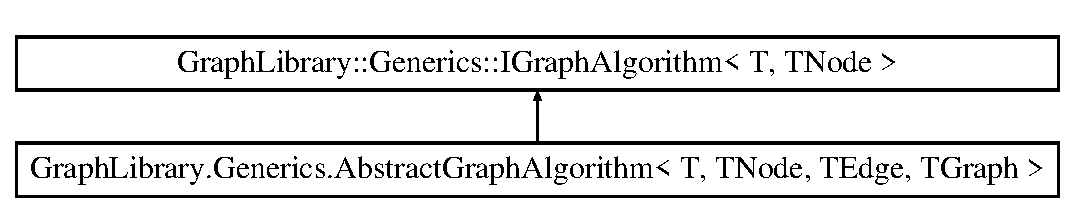
\includegraphics[height=2.000000cm]{class_graph_library_1_1_generics_1_1_abstract_graph_algorithm}
\end{center}
\end{figure}
\subsection*{Public Member Functions}
\begin{DoxyCompactItemize}
\item 
abstract void \hyperlink{class_graph_library_1_1_generics_1_1_abstract_graph_algorithm_a0e98ca6c259123c6975b20857c4af7be}{Init} ()
\begin{DoxyCompactList}\small\item\em Initializes the algorithm. The client writes code in this function in the subclasses to initialize the algorithm \end{DoxyCompactList}\item 
virtual T \hyperlink{class_graph_library_1_1_generics_1_1_abstract_graph_algorithm_a08ce42bc60d311959bc5d1293d3c63da}{Visit} (T\+Node node)
\begin{DoxyCompactList}\small\item\em The Visit method refers to the action the algorithm performs to a specific node This function can be called either recursively or iteratively \end{DoxyCompactList}\item 
virtual T \hyperlink{class_graph_library_1_1_generics_1_1_abstract_graph_algorithm_ad40868c545ebd337122c84f02238b2db}{Visit} (T\+Edge edge)
\begin{DoxyCompactList}\small\item\em Visits the specified edge and performs the algorithmic action on it. \end{DoxyCompactList}\item 
abstract object \hyperlink{class_graph_library_1_1_generics_1_1_abstract_graph_algorithm_afe8f7c1f5bf5085b31a59139d6034eba}{Visit\+Children} (T\+Node node)
\begin{DoxyCompactList}\small\item\em Visits the children of the specified node. Call this function if nothing is necessesary to be done in the current node apart from visiting its children \end{DoxyCompactList}\item 
object \hyperlink{class_graph_library_1_1_generics_1_1_abstract_graph_algorithm_a229680ade697cc543951b56f2d7857b2}{Info} (T\+Node node, object key=null)
\begin{DoxyCompactList}\small\item\em Returns information concerning a node or a graph ( derives from node) Since the graph derives from \hyperlink{class_graph_library_1_1_c_graph_node}{C\+Graph\+Node} it stores the information at the same collection as node. So the function to retrieve the information is common in both elements \end{DoxyCompactList}\item 
object \hyperlink{class_graph_library_1_1_generics_1_1_abstract_graph_algorithm_a058caf0df4003a1336385f5d0c483023}{Info} (T\+Edge edge, object key=null)
\begin{DoxyCompactList}\small\item\em Returns the information of the specified edge \end{DoxyCompactList}\item 
object \hyperlink{class_graph_library_1_1_generics_1_1_abstract_graph_algorithm_a5e7832df95cf65108e8a1006b83251a0}{Info} (T\+Node source, T\+Node target, object key=null)
\begin{DoxyCompactList}\small\item\em Returns the information of the edge between the given source and target nodes. \end{DoxyCompactList}\item 
void \hyperlink{class_graph_library_1_1_generics_1_1_abstract_graph_algorithm_a2eae65a9111672ba14a6f992659ad47e}{Create\+Info} (T\+Node node, object info, object key=null)
\begin{DoxyCompactList}\small\item\em Stores the information at the specified node or graph. If information already exists, it is overwritten \end{DoxyCompactList}\item 
void \hyperlink{class_graph_library_1_1_generics_1_1_abstract_graph_algorithm_a17ed5f51aeb7550e989279f60875a3ee}{Create\+Info} (T\+Edge edge, object info, object key=null)
\begin{DoxyCompactList}\small\item\em Stores the information at the specified edge. If information already exists, it is overwritten \end{DoxyCompactList}\item 
void \hyperlink{class_graph_library_1_1_generics_1_1_abstract_graph_algorithm_a1c1e9c16c3303fd647af598cc1bbecb8}{Create\+Info} (T\+Node source, T\+Node target, object info, object key=null)
\begin{DoxyCompactList}\small\item\em Stores the information at the specified edge. If information already exists, it is overwritten \end{DoxyCompactList}\end{DoxyCompactItemize}
\subsection*{Protected Member Functions}
\begin{DoxyCompactItemize}
\item 
\hyperlink{class_graph_library_1_1_generics_1_1_abstract_graph_algorithm_aeff19bab0aa2fd277ad17190ac826472}{Abstract\+Graph\+Algorithm} (T\+Graph graph, \hyperlink{class_graph_library_1_1_generics_1_1_abstract_graph_query_info}{Abstract\+Graph\+Query\+Info}$<$ T\+Node, T\+Edge, T\+Graph $>$ info, \hyperlink{class_graph_library_1_1_generics_1_1_abstract_graph_iterator_factory}{Abstract\+Graph\+Iterator\+Factory}$<$ T\+Node, T\+Edge, T\+Graph $>$ iterator\+Factory)
\begin{DoxyCompactList}\small\item\em Initializes a new instance of the \hyperlink{class_graph_library_1_1_generics_1_1_abstract_graph_algorithm_aeff19bab0aa2fd277ad17190ac826472}{Abstract\+Graph\+Algorithm$<$\+T$>$} class. \end{DoxyCompactList}\end{DoxyCompactItemize}
\subsection*{Protected Attributes}
\begin{DoxyCompactItemize}
\item 
T\+Graph \hyperlink{class_graph_library_1_1_generics_1_1_abstract_graph_algorithm_a11916e5c10f7a5b827c3ad8425becdf3}{m\+\_\+\+Graph}
\begin{DoxyCompactList}\small\item\em A reference to the graph to which the algorithm is applied \end{DoxyCompactList}\item 
\hyperlink{class_graph_library_1_1_generics_1_1_abstract_graph_query_info}{Abstract\+Graph\+Query\+Info}$<$ T\+Node, T\+Edge, T\+Graph $>$ \hyperlink{class_graph_library_1_1_generics_1_1_abstract_graph_algorithm_ad93dc80869889f95dd6588d6a07703d7}{m\+\_\+\+Info}
\begin{DoxyCompactList}\small\item\em The mediator which provides the information (of nodes, edges, graph) to the algorithm from where it is stored. It is based on the bridge design pattern. The purpose of this class is to separate the implementation of the graph from the algorithm. \end{DoxyCompactList}\item 
\hyperlink{class_graph_library_1_1_generics_1_1_abstract_graph_iterator_factory}{Abstract\+Graph\+Iterator\+Factory}$<$ T\+Node, T\+Edge, T\+Graph $>$ \hyperlink{class_graph_library_1_1_generics_1_1_abstract_graph_algorithm_a1f64fc66f6f6ccef709df92d3e6081b2}{m\+\_\+\+Iterator\+Factory}
\begin{DoxyCompactList}\small\item\em The iterator factory \end{DoxyCompactList}\end{DoxyCompactItemize}


\subsection{Detailed Description}
The abstract base class of the algorithms applied on graphs 


\begin{DoxyTemplParams}{Template Parameters}
{\em T} & Visit function retured type\\
\hline
{\em Node} & The type of the node.\\
\hline
{\em Edge} & The type of the edge.\\
\hline
{\em Graph} & The type of the Graph.\\
\hline
\end{DoxyTemplParams}
\begin{DoxySeeAlso}{See also}
Graph\+Library.\+Generics.\+I\+Graph\+Algorithm$<$\+T,\+Node$>$, I\+Graph\+Algorithm$<$\+T,\+Node$>$, I\+Graph\+Algorithm$<$\+T,\+Node$>$


\end{DoxySeeAlso}


\subsection{Constructor \& Destructor Documentation}
\hypertarget{class_graph_library_1_1_generics_1_1_abstract_graph_algorithm_aeff19bab0aa2fd277ad17190ac826472}{}\index{Graph\+Library\+::\+Generics\+::\+Abstract\+Graph\+Algorithm@{Graph\+Library\+::\+Generics\+::\+Abstract\+Graph\+Algorithm}!Abstract\+Graph\+Algorithm@{Abstract\+Graph\+Algorithm}}
\index{Abstract\+Graph\+Algorithm@{Abstract\+Graph\+Algorithm}!Graph\+Library\+::\+Generics\+::\+Abstract\+Graph\+Algorithm@{Graph\+Library\+::\+Generics\+::\+Abstract\+Graph\+Algorithm}}
\subsubsection[{Abstract\+Graph\+Algorithm(\+T\+Graph graph, Abstract\+Graph\+Query\+Info$<$ T\+Node, T\+Edge, T\+Graph $>$ info, Abstract\+Graph\+Iterator\+Factory$<$ T\+Node, T\+Edge, T\+Graph $>$ iterator\+Factory)}]{\setlength{\rightskip}{0pt plus 5cm}{\bf Graph\+Library.\+Generics.\+Abstract\+Graph\+Algorithm}$<$ T, T\+Node, T\+Edge, T\+Graph $>$.{\bf Abstract\+Graph\+Algorithm} (
\begin{DoxyParamCaption}
\item[{T\+Graph}]{graph, }
\item[{{\bf Abstract\+Graph\+Query\+Info}$<$ T\+Node, T\+Edge, T\+Graph $>$}]{info, }
\item[{{\bf Abstract\+Graph\+Iterator\+Factory}$<$ T\+Node, T\+Edge, T\+Graph $>$}]{iterator\+Factory}
\end{DoxyParamCaption}
)\hspace{0.3cm}{\ttfamily [protected]}}\label{class_graph_library_1_1_generics_1_1_abstract_graph_algorithm_aeff19bab0aa2fd277ad17190ac826472}


Initializes a new instance of the \hyperlink{class_graph_library_1_1_generics_1_1_abstract_graph_algorithm_aeff19bab0aa2fd277ad17190ac826472}{Abstract\+Graph\+Algorithm$<$\+T$>$} class. 


\begin{DoxyParams}{Parameters}
{\em graph} & The graph.\\
\hline
{\em info} & The information object.\\
\hline
\end{DoxyParams}


\subsection{Member Function Documentation}
\hypertarget{class_graph_library_1_1_generics_1_1_abstract_graph_algorithm_a2eae65a9111672ba14a6f992659ad47e}{}\index{Graph\+Library\+::\+Generics\+::\+Abstract\+Graph\+Algorithm@{Graph\+Library\+::\+Generics\+::\+Abstract\+Graph\+Algorithm}!Create\+Info@{Create\+Info}}
\index{Create\+Info@{Create\+Info}!Graph\+Library\+::\+Generics\+::\+Abstract\+Graph\+Algorithm@{Graph\+Library\+::\+Generics\+::\+Abstract\+Graph\+Algorithm}}
\subsubsection[{Create\+Info(\+T\+Node node, object info, object key=null)}]{\setlength{\rightskip}{0pt plus 5cm}void {\bf Graph\+Library.\+Generics.\+Abstract\+Graph\+Algorithm}$<$ T, T\+Node, T\+Edge, T\+Graph $>$.Create\+Info (
\begin{DoxyParamCaption}
\item[{T\+Node}]{node, }
\item[{object}]{info, }
\item[{object}]{key = {\ttfamily null}}
\end{DoxyParamCaption}
)}\label{class_graph_library_1_1_generics_1_1_abstract_graph_algorithm_a2eae65a9111672ba14a6f992659ad47e}


Stores the information at the specified node or graph. If information already exists, it is overwritten 


\begin{DoxyParams}{Parameters}
{\em node} & The node.\\
\hline
{\em info} & The information object\\
\hline
{\em key} & The key to the edge information. Can be algorithm, iterator etc.\\
\hline
\end{DoxyParams}
example \+: A D\+F\+S graph algorithm \char`\"{}this\char`\"{} can assign a information record \char`\"{}info\char`\"{} to a \char`\"{}node\char`\"{} example \+: Create\+Info(itg.\+M\+\_\+\+Current\+Item,new Edge\+Info\+\_\+\+D\+F\+S(0),this); \hypertarget{class_graph_library_1_1_generics_1_1_abstract_graph_algorithm_a17ed5f51aeb7550e989279f60875a3ee}{}\index{Graph\+Library\+::\+Generics\+::\+Abstract\+Graph\+Algorithm@{Graph\+Library\+::\+Generics\+::\+Abstract\+Graph\+Algorithm}!Create\+Info@{Create\+Info}}
\index{Create\+Info@{Create\+Info}!Graph\+Library\+::\+Generics\+::\+Abstract\+Graph\+Algorithm@{Graph\+Library\+::\+Generics\+::\+Abstract\+Graph\+Algorithm}}
\subsubsection[{Create\+Info(\+T\+Edge edge, object info, object key=null)}]{\setlength{\rightskip}{0pt plus 5cm}void {\bf Graph\+Library.\+Generics.\+Abstract\+Graph\+Algorithm}$<$ T, T\+Node, T\+Edge, T\+Graph $>$.Create\+Info (
\begin{DoxyParamCaption}
\item[{T\+Edge}]{edge, }
\item[{object}]{info, }
\item[{object}]{key = {\ttfamily null}}
\end{DoxyParamCaption}
)}\label{class_graph_library_1_1_generics_1_1_abstract_graph_algorithm_a17ed5f51aeb7550e989279f60875a3ee}


Stores the information at the specified edge. If information already exists, it is overwritten 


\begin{DoxyParams}{Parameters}
{\em edge} & The edge.\\
\hline
{\em info} & The information object\\
\hline
{\em key} & The key to the edge information. Can be algorithm, iterator etc.\\
\hline
\end{DoxyParams}
\hypertarget{class_graph_library_1_1_generics_1_1_abstract_graph_algorithm_a1c1e9c16c3303fd647af598cc1bbecb8}{}\index{Graph\+Library\+::\+Generics\+::\+Abstract\+Graph\+Algorithm@{Graph\+Library\+::\+Generics\+::\+Abstract\+Graph\+Algorithm}!Create\+Info@{Create\+Info}}
\index{Create\+Info@{Create\+Info}!Graph\+Library\+::\+Generics\+::\+Abstract\+Graph\+Algorithm@{Graph\+Library\+::\+Generics\+::\+Abstract\+Graph\+Algorithm}}
\subsubsection[{Create\+Info(\+T\+Node source, T\+Node target, object info, object key=null)}]{\setlength{\rightskip}{0pt plus 5cm}void {\bf Graph\+Library.\+Generics.\+Abstract\+Graph\+Algorithm}$<$ T, T\+Node, T\+Edge, T\+Graph $>$.Create\+Info (
\begin{DoxyParamCaption}
\item[{T\+Node}]{source, }
\item[{T\+Node}]{target, }
\item[{object}]{info, }
\item[{object}]{key = {\ttfamily null}}
\end{DoxyParamCaption}
)}\label{class_graph_library_1_1_generics_1_1_abstract_graph_algorithm_a1c1e9c16c3303fd647af598cc1bbecb8}


Stores the information at the specified edge. If information already exists, it is overwritten 


\begin{DoxyParams}{Parameters}
{\em source} & The source node.\\
\hline
{\em target} & The target node.\\
\hline
{\em info} & The information object\\
\hline
{\em key} & The key to the edge information. Can be algorithm, iterator etc.\\
\hline
\end{DoxyParams}
\hypertarget{class_graph_library_1_1_generics_1_1_abstract_graph_algorithm_a229680ade697cc543951b56f2d7857b2}{}\index{Graph\+Library\+::\+Generics\+::\+Abstract\+Graph\+Algorithm@{Graph\+Library\+::\+Generics\+::\+Abstract\+Graph\+Algorithm}!Info@{Info}}
\index{Info@{Info}!Graph\+Library\+::\+Generics\+::\+Abstract\+Graph\+Algorithm@{Graph\+Library\+::\+Generics\+::\+Abstract\+Graph\+Algorithm}}
\subsubsection[{Info(\+T\+Node node, object key=null)}]{\setlength{\rightskip}{0pt plus 5cm}object {\bf Graph\+Library.\+Generics.\+Abstract\+Graph\+Algorithm}$<$ T, T\+Node, T\+Edge, T\+Graph $>$.Info (
\begin{DoxyParamCaption}
\item[{T\+Node}]{node, }
\item[{object}]{key = {\ttfamily null}}
\end{DoxyParamCaption}
)}\label{class_graph_library_1_1_generics_1_1_abstract_graph_algorithm_a229680ade697cc543951b56f2d7857b2}


Returns information concerning a node or a graph ( derives from node) Since the graph derives from \hyperlink{class_graph_library_1_1_c_graph_node}{C\+Graph\+Node} it stores the information at the same collection as node. So the function to retrieve the information is common in both elements 


\begin{DoxyParams}{Parameters}
{\em node} & The node.\\
\hline
{\em key} & The key to the node information. Can be algorithm, iterator etc.\\
\hline
\end{DoxyParams}
\begin{DoxyReturn}{Returns}
The information object
\end{DoxyReturn}
\hypertarget{class_graph_library_1_1_generics_1_1_abstract_graph_algorithm_a058caf0df4003a1336385f5d0c483023}{}\index{Graph\+Library\+::\+Generics\+::\+Abstract\+Graph\+Algorithm@{Graph\+Library\+::\+Generics\+::\+Abstract\+Graph\+Algorithm}!Info@{Info}}
\index{Info@{Info}!Graph\+Library\+::\+Generics\+::\+Abstract\+Graph\+Algorithm@{Graph\+Library\+::\+Generics\+::\+Abstract\+Graph\+Algorithm}}
\subsubsection[{Info(\+T\+Edge edge, object key=null)}]{\setlength{\rightskip}{0pt plus 5cm}object {\bf Graph\+Library.\+Generics.\+Abstract\+Graph\+Algorithm}$<$ T, T\+Node, T\+Edge, T\+Graph $>$.Info (
\begin{DoxyParamCaption}
\item[{T\+Edge}]{edge, }
\item[{object}]{key = {\ttfamily null}}
\end{DoxyParamCaption}
)}\label{class_graph_library_1_1_generics_1_1_abstract_graph_algorithm_a058caf0df4003a1336385f5d0c483023}


Returns the information of the specified edge 


\begin{DoxyParams}{Parameters}
{\em edge} & The edge.\\
\hline
{\em key} & The key to the edge information. Can be algorithm, iterator etc.\\
\hline
\end{DoxyParams}
\begin{DoxyReturn}{Returns}
The information object
\end{DoxyReturn}
\hypertarget{class_graph_library_1_1_generics_1_1_abstract_graph_algorithm_a5e7832df95cf65108e8a1006b83251a0}{}\index{Graph\+Library\+::\+Generics\+::\+Abstract\+Graph\+Algorithm@{Graph\+Library\+::\+Generics\+::\+Abstract\+Graph\+Algorithm}!Info@{Info}}
\index{Info@{Info}!Graph\+Library\+::\+Generics\+::\+Abstract\+Graph\+Algorithm@{Graph\+Library\+::\+Generics\+::\+Abstract\+Graph\+Algorithm}}
\subsubsection[{Info(\+T\+Node source, T\+Node target, object key=null)}]{\setlength{\rightskip}{0pt plus 5cm}object {\bf Graph\+Library.\+Generics.\+Abstract\+Graph\+Algorithm}$<$ T, T\+Node, T\+Edge, T\+Graph $>$.Info (
\begin{DoxyParamCaption}
\item[{T\+Node}]{source, }
\item[{T\+Node}]{target, }
\item[{object}]{key = {\ttfamily null}}
\end{DoxyParamCaption}
)}\label{class_graph_library_1_1_generics_1_1_abstract_graph_algorithm_a5e7832df95cf65108e8a1006b83251a0}


Returns the information of the edge between the given source and target nodes. 


\begin{DoxyParams}{Parameters}
{\em source} & The source.\\
\hline
{\em target} & The target.\\
\hline
{\em key} & The key to the edge information. Can be algorithm, iterator etc.\\
\hline
\end{DoxyParams}
\begin{DoxyReturn}{Returns}
The information object
\end{DoxyReturn}
\hypertarget{class_graph_library_1_1_generics_1_1_abstract_graph_algorithm_a0e98ca6c259123c6975b20857c4af7be}{}\index{Graph\+Library\+::\+Generics\+::\+Abstract\+Graph\+Algorithm@{Graph\+Library\+::\+Generics\+::\+Abstract\+Graph\+Algorithm}!Init@{Init}}
\index{Init@{Init}!Graph\+Library\+::\+Generics\+::\+Abstract\+Graph\+Algorithm@{Graph\+Library\+::\+Generics\+::\+Abstract\+Graph\+Algorithm}}
\subsubsection[{Init()}]{\setlength{\rightskip}{0pt plus 5cm}abstract void {\bf Graph\+Library.\+Generics.\+Abstract\+Graph\+Algorithm}$<$ T, T\+Node, T\+Edge, T\+Graph $>$.Init (
\begin{DoxyParamCaption}
{}
\end{DoxyParamCaption}
)\hspace{0.3cm}{\ttfamily [pure virtual]}}\label{class_graph_library_1_1_generics_1_1_abstract_graph_algorithm_a0e98ca6c259123c6975b20857c4af7be}


Initializes the algorithm. The client writes code in this function in the subclasses to initialize the algorithm 

\hypertarget{class_graph_library_1_1_generics_1_1_abstract_graph_algorithm_a08ce42bc60d311959bc5d1293d3c63da}{}\index{Graph\+Library\+::\+Generics\+::\+Abstract\+Graph\+Algorithm@{Graph\+Library\+::\+Generics\+::\+Abstract\+Graph\+Algorithm}!Visit@{Visit}}
\index{Visit@{Visit}!Graph\+Library\+::\+Generics\+::\+Abstract\+Graph\+Algorithm@{Graph\+Library\+::\+Generics\+::\+Abstract\+Graph\+Algorithm}}
\subsubsection[{Visit(\+T\+Node node)}]{\setlength{\rightskip}{0pt plus 5cm}virtual T {\bf Graph\+Library.\+Generics.\+Abstract\+Graph\+Algorithm}$<$ T, T\+Node, T\+Edge, T\+Graph $>$.Visit (
\begin{DoxyParamCaption}
\item[{T\+Node}]{node}
\end{DoxyParamCaption}
)\hspace{0.3cm}{\ttfamily [virtual]}}\label{class_graph_library_1_1_generics_1_1_abstract_graph_algorithm_a08ce42bc60d311959bc5d1293d3c63da}


The Visit method refers to the action the algorithm performs to a specific node This function can be called either recursively or iteratively 


\begin{DoxyParams}{Parameters}
{\em node} & The node to which the algorithm acts.\\
\hline
\end{DoxyParams}
\begin{DoxyReturn}{Returns}
The parameter refers to the type of the return result 
\end{DoxyReturn}


Implements \hyperlink{interface_graph_library_1_1_generics_1_1_i_graph_algorithm_a8bc65da7e1004a5c55f75b57872fad31}{Graph\+Library.\+Generics.\+I\+Graph\+Algorithm$<$ T, T\+Node $>$}.

\hypertarget{class_graph_library_1_1_generics_1_1_abstract_graph_algorithm_ad40868c545ebd337122c84f02238b2db}{}\index{Graph\+Library\+::\+Generics\+::\+Abstract\+Graph\+Algorithm@{Graph\+Library\+::\+Generics\+::\+Abstract\+Graph\+Algorithm}!Visit@{Visit}}
\index{Visit@{Visit}!Graph\+Library\+::\+Generics\+::\+Abstract\+Graph\+Algorithm@{Graph\+Library\+::\+Generics\+::\+Abstract\+Graph\+Algorithm}}
\subsubsection[{Visit(\+T\+Edge edge)}]{\setlength{\rightskip}{0pt plus 5cm}virtual T {\bf Graph\+Library.\+Generics.\+Abstract\+Graph\+Algorithm}$<$ T, T\+Node, T\+Edge, T\+Graph $>$.Visit (
\begin{DoxyParamCaption}
\item[{T\+Edge}]{edge}
\end{DoxyParamCaption}
)\hspace{0.3cm}{\ttfamily [virtual]}}\label{class_graph_library_1_1_generics_1_1_abstract_graph_algorithm_ad40868c545ebd337122c84f02238b2db}


Visits the specified edge and performs the algorithmic action on it. 


\begin{DoxyParams}{Parameters}
{\em edge} & The edge to which the algorithm acts\\
\hline
\end{DoxyParams}
\begin{DoxyReturn}{Returns}

\end{DoxyReturn}
\hypertarget{class_graph_library_1_1_generics_1_1_abstract_graph_algorithm_afe8f7c1f5bf5085b31a59139d6034eba}{}\index{Graph\+Library\+::\+Generics\+::\+Abstract\+Graph\+Algorithm@{Graph\+Library\+::\+Generics\+::\+Abstract\+Graph\+Algorithm}!Visit\+Children@{Visit\+Children}}
\index{Visit\+Children@{Visit\+Children}!Graph\+Library\+::\+Generics\+::\+Abstract\+Graph\+Algorithm@{Graph\+Library\+::\+Generics\+::\+Abstract\+Graph\+Algorithm}}
\subsubsection[{Visit\+Children(\+T\+Node node)}]{\setlength{\rightskip}{0pt plus 5cm}abstract object {\bf Graph\+Library.\+Generics.\+Abstract\+Graph\+Algorithm}$<$ T, T\+Node, T\+Edge, T\+Graph $>$.Visit\+Children (
\begin{DoxyParamCaption}
\item[{T\+Node}]{node}
\end{DoxyParamCaption}
)\hspace{0.3cm}{\ttfamily [pure virtual]}}\label{class_graph_library_1_1_generics_1_1_abstract_graph_algorithm_afe8f7c1f5bf5085b31a59139d6034eba}


Visits the children of the specified node. Call this function if nothing is necessesary to be done in the current node apart from visiting its children 


\begin{DoxyParams}{Parameters}
{\em node} & The node to which the children is visited\\
\hline
\end{DoxyParams}
\begin{DoxyReturn}{Returns}
The default version returns null 
\end{DoxyReturn}


Implements \hyperlink{interface_graph_library_1_1_generics_1_1_i_graph_algorithm_aa8576b6860d0047bfd491c3101e876cc}{Graph\+Library.\+Generics.\+I\+Graph\+Algorithm$<$ T, T\+Node $>$}.



\subsection{Member Data Documentation}
\hypertarget{class_graph_library_1_1_generics_1_1_abstract_graph_algorithm_a11916e5c10f7a5b827c3ad8425becdf3}{}\index{Graph\+Library\+::\+Generics\+::\+Abstract\+Graph\+Algorithm@{Graph\+Library\+::\+Generics\+::\+Abstract\+Graph\+Algorithm}!m\+\_\+\+Graph@{m\+\_\+\+Graph}}
\index{m\+\_\+\+Graph@{m\+\_\+\+Graph}!Graph\+Library\+::\+Generics\+::\+Abstract\+Graph\+Algorithm@{Graph\+Library\+::\+Generics\+::\+Abstract\+Graph\+Algorithm}}
\subsubsection[{m\+\_\+\+Graph}]{\setlength{\rightskip}{0pt plus 5cm}T\+Graph {\bf Graph\+Library.\+Generics.\+Abstract\+Graph\+Algorithm}$<$ T, T\+Node, T\+Edge, T\+Graph $>$.m\+\_\+\+Graph\hspace{0.3cm}{\ttfamily [protected]}}\label{class_graph_library_1_1_generics_1_1_abstract_graph_algorithm_a11916e5c10f7a5b827c3ad8425becdf3}


A reference to the graph to which the algorithm is applied 

\hypertarget{class_graph_library_1_1_generics_1_1_abstract_graph_algorithm_ad93dc80869889f95dd6588d6a07703d7}{}\index{Graph\+Library\+::\+Generics\+::\+Abstract\+Graph\+Algorithm@{Graph\+Library\+::\+Generics\+::\+Abstract\+Graph\+Algorithm}!m\+\_\+\+Info@{m\+\_\+\+Info}}
\index{m\+\_\+\+Info@{m\+\_\+\+Info}!Graph\+Library\+::\+Generics\+::\+Abstract\+Graph\+Algorithm@{Graph\+Library\+::\+Generics\+::\+Abstract\+Graph\+Algorithm}}
\subsubsection[{m\+\_\+\+Info}]{\setlength{\rightskip}{0pt plus 5cm}{\bf Abstract\+Graph\+Query\+Info}$<$T\+Node,T\+Edge,T\+Graph$>$ {\bf Graph\+Library.\+Generics.\+Abstract\+Graph\+Algorithm}$<$ T, T\+Node, T\+Edge, T\+Graph $>$.m\+\_\+\+Info\hspace{0.3cm}{\ttfamily [protected]}}\label{class_graph_library_1_1_generics_1_1_abstract_graph_algorithm_ad93dc80869889f95dd6588d6a07703d7}


The mediator which provides the information (of nodes, edges, graph) to the algorithm from where it is stored. It is based on the bridge design pattern. The purpose of this class is to separate the implementation of the graph from the algorithm. 

\hypertarget{class_graph_library_1_1_generics_1_1_abstract_graph_algorithm_a1f64fc66f6f6ccef709df92d3e6081b2}{}\index{Graph\+Library\+::\+Generics\+::\+Abstract\+Graph\+Algorithm@{Graph\+Library\+::\+Generics\+::\+Abstract\+Graph\+Algorithm}!m\+\_\+\+Iterator\+Factory@{m\+\_\+\+Iterator\+Factory}}
\index{m\+\_\+\+Iterator\+Factory@{m\+\_\+\+Iterator\+Factory}!Graph\+Library\+::\+Generics\+::\+Abstract\+Graph\+Algorithm@{Graph\+Library\+::\+Generics\+::\+Abstract\+Graph\+Algorithm}}
\subsubsection[{m\+\_\+\+Iterator\+Factory}]{\setlength{\rightskip}{0pt plus 5cm}{\bf Abstract\+Graph\+Iterator\+Factory}$<$T\+Node, T\+Edge, T\+Graph$>$ {\bf Graph\+Library.\+Generics.\+Abstract\+Graph\+Algorithm}$<$ T, T\+Node, T\+Edge, T\+Graph $>$.m\+\_\+\+Iterator\+Factory\hspace{0.3cm}{\ttfamily [protected]}}\label{class_graph_library_1_1_generics_1_1_abstract_graph_algorithm_a1f64fc66f6f6ccef709df92d3e6081b2}


The iterator factory 



The documentation for this class was generated from the following file\+:\begin{DoxyCompactItemize}
\item 
Graph\+Library/\+Generics/Abstract\+Graph\+Algorithm.\+cs\end{DoxyCompactItemize}

\hypertarget{class_graph_library_1_1_generics_1_1_abstract_graph_iterator}{}\section{Graph\+Library.\+Generics.\+Abstract\+Graph\+Iterator$<$ T $>$ Class Template Reference}
\label{class_graph_library_1_1_generics_1_1_abstract_graph_iterator}\index{Graph\+Library.\+Generics.\+Abstract\+Graph\+Iterator$<$ T $>$@{Graph\+Library.\+Generics.\+Abstract\+Graph\+Iterator$<$ T $>$}}


This class is the base abstract class of Graph\+Iterators. It has no implementation except from the m\+\_\+current\+Item member variable. This variable always point to the current element (which has type T) that the iterator points. The class\textquotesingle{}s methods are executed in a specific sequence that is dictated by the loop statement semantics that is \hyperlink{class_graph_library_1_1_generics_1_1_abstract_graph_iterator_a2c97c7a412c233b8442b7ad403f29779}{Begin()}, \hyperlink{class_graph_library_1_1_generics_1_1_abstract_graph_iterator_aa8cd9f596ec0b6c4c1e9c244ba75df04}{End()}, L\+O\+O\+P\+\_\+\+B\+O\+D\+Y, \hyperlink{class_graph_library_1_1_generics_1_1_abstract_graph_iterator_aac8cffd0d579708a94ba056e4f4a00b2}{Next()}, \hyperlink{class_graph_library_1_1_generics_1_1_abstract_graph_iterator_aa8cd9f596ec0b6c4c1e9c244ba75df04}{End()}, L\+O\+O\+P\+\_\+\+B\+O\+D\+Y, \hyperlink{class_graph_library_1_1_generics_1_1_abstract_graph_iterator_aac8cffd0d579708a94ba056e4f4a00b2}{Next()}, \hyperlink{class_graph_library_1_1_generics_1_1_abstract_graph_iterator_aa8cd9f596ec0b6c4c1e9c244ba75df04}{End()}, L\+O\+O\+P\+\_\+\+B\+O\+D\+Y, \hyperlink{class_graph_library_1_1_generics_1_1_abstract_graph_iterator_aac8cffd0d579708a94ba056e4f4a00b2}{Next()}, \hyperlink{class_graph_library_1_1_generics_1_1_abstract_graph_iterator_aa8cd9f596ec0b6c4c1e9c244ba75df04}{End()}... etc  


Inheritance diagram for Graph\+Library.\+Generics.\+Abstract\+Graph\+Iterator$<$ T $>$\+:\begin{figure}[H]
\begin{center}
\leavevmode
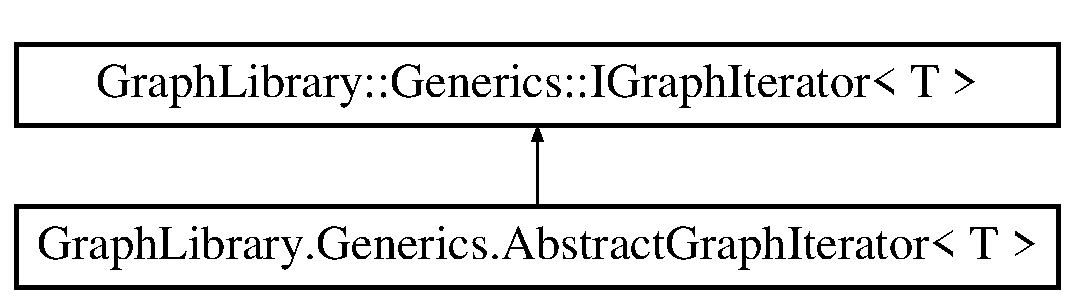
\includegraphics[height=2.000000cm]{class_graph_library_1_1_generics_1_1_abstract_graph_iterator}
\end{center}
\end{figure}
\subsection*{Public Member Functions}
\begin{DoxyCompactItemize}
\item 
abstract T \hyperlink{class_graph_library_1_1_generics_1_1_abstract_graph_iterator_a2c97c7a412c233b8442b7ad403f29779}{Begin} ()
\begin{DoxyCompactList}\small\item\em Executes once at the start of the iteration and before the \hyperlink{class_graph_library_1_1_generics_1_1_abstract_graph_iterator_aa8cd9f596ec0b6c4c1e9c244ba75df04}{End()} method Initializes the iterator variable ( realized in the subclasses ) and the m\+\_\+current\+Item to point to the first element of the item set. If the set is empty the m\+\_\+current\+Item points to null. After the \hyperlink{class_graph_library_1_1_generics_1_1_abstract_graph_iterator_a2c97c7a412c233b8442b7ad403f29779}{Begin()} method the \hyperlink{class_graph_library_1_1_generics_1_1_abstract_graph_iterator_aa8cd9f596ec0b6c4c1e9c244ba75df04}{End()} method executes before going into the loop body. Thus the loop terminates if the item set is empty before ever running the loop body The transition logic for finding the first item in the items set is implemented in the subclasses \end{DoxyCompactList}\item 
abstract bool \hyperlink{class_graph_library_1_1_generics_1_1_abstract_graph_iterator_aa8cd9f596ec0b6c4c1e9c244ba75df04}{End} ()
\begin{DoxyCompactList}\small\item\em Executes after the \hyperlink{class_graph_library_1_1_generics_1_1_abstract_graph_iterator_a2c97c7a412c233b8442b7ad403f29779}{Begin()} or \hyperlink{class_graph_library_1_1_generics_1_1_abstract_graph_iterator_aac8cffd0d579708a94ba056e4f4a00b2}{Next()} methods and before the Loop Body Returns true if the m\+\_\+current\+Item is null. This case arises in the following scenarios\+: 1) The item set is empty thus, after the \hyperlink{class_graph_library_1_1_generics_1_1_abstract_graph_iterator_a2c97c7a412c233b8442b7ad403f29779}{Begin()} method call the \hyperlink{class_graph_library_1_1_generics_1_1_abstract_graph_iterator_aa8cd9f596ec0b6c4c1e9c244ba75df04}{End()} identifies that m\+\_\+current\+Item points to null 2) The item set is not empty and the iterator went outside the boundaries of the item set after the call to \hyperlink{class_graph_library_1_1_generics_1_1_abstract_graph_iterator_aac8cffd0d579708a94ba056e4f4a00b2}{Next()} method (\hyperlink{class_graph_library_1_1_generics_1_1_abstract_graph_iterator_aac8cffd0d579708a94ba056e4f4a00b2}{Next()} method set m\+\_\+current\+Item to null) \end{DoxyCompactList}\item 
abstract T \hyperlink{class_graph_library_1_1_generics_1_1_abstract_graph_iterator_aac8cffd0d579708a94ba056e4f4a00b2}{Next} ()
\begin{DoxyCompactList}\small\item\em Executes after the execution of the loop body and before the \hyperlink{class_graph_library_1_1_generics_1_1_abstract_graph_iterator_aa8cd9f596ec0b6c4c1e9c244ba75df04}{End()} method Increases the iteration variable and set the m\+\_\+current\+Item to point to the current item of the item set. In case where the end of the item set is reached the m\+\_\+current\+Item points to null which is identified by the \hyperlink{class_graph_library_1_1_generics_1_1_abstract_graph_iterator_aa8cd9f596ec0b6c4c1e9c244ba75df04}{End()} methods that is executed next. The transition logic from item to item is implemented from the subclasses. \end{DoxyCompactList}\end{DoxyCompactItemize}
\subsection*{Protected Attributes}
\begin{DoxyCompactItemize}
\item 
T \hyperlink{class_graph_library_1_1_generics_1_1_abstract_graph_iterator_a19c7904539e8519162a4c42739d37757}{m\+\_\+current\+Item} = default(T)
\begin{DoxyCompactList}\small\item\em Current node pointed to by the iterator \end{DoxyCompactList}\end{DoxyCompactItemize}
\subsection*{Properties}
\begin{DoxyCompactItemize}
\item 
T \hyperlink{class_graph_library_1_1_generics_1_1_abstract_graph_iterator_a6621ff4270d662b95a80c7cbcc75b68c}{M\+\_\+\+Current\+Item}\hspace{0.3cm}{\ttfamily  \mbox{[}get\mbox{]}}
\begin{DoxyCompactList}\small\item\em Returns the current item pointed by the iterator \end{DoxyCompactList}\end{DoxyCompactItemize}


\subsection{Detailed Description}
This class is the base abstract class of Graph\+Iterators. It has no implementation except from the m\+\_\+current\+Item member variable. This variable always point to the current element (which has type T) that the iterator points. The class\textquotesingle{}s methods are executed in a specific sequence that is dictated by the loop statement semantics that is \hyperlink{class_graph_library_1_1_generics_1_1_abstract_graph_iterator_a2c97c7a412c233b8442b7ad403f29779}{Begin()}, \hyperlink{class_graph_library_1_1_generics_1_1_abstract_graph_iterator_aa8cd9f596ec0b6c4c1e9c244ba75df04}{End()}, L\+O\+O\+P\+\_\+\+B\+O\+D\+Y, \hyperlink{class_graph_library_1_1_generics_1_1_abstract_graph_iterator_aac8cffd0d579708a94ba056e4f4a00b2}{Next()}, \hyperlink{class_graph_library_1_1_generics_1_1_abstract_graph_iterator_aa8cd9f596ec0b6c4c1e9c244ba75df04}{End()}, L\+O\+O\+P\+\_\+\+B\+O\+D\+Y, \hyperlink{class_graph_library_1_1_generics_1_1_abstract_graph_iterator_aac8cffd0d579708a94ba056e4f4a00b2}{Next()}, \hyperlink{class_graph_library_1_1_generics_1_1_abstract_graph_iterator_aa8cd9f596ec0b6c4c1e9c244ba75df04}{End()}, L\+O\+O\+P\+\_\+\+B\+O\+D\+Y, \hyperlink{class_graph_library_1_1_generics_1_1_abstract_graph_iterator_aac8cffd0d579708a94ba056e4f4a00b2}{Next()}, \hyperlink{class_graph_library_1_1_generics_1_1_abstract_graph_iterator_aa8cd9f596ec0b6c4c1e9c244ba75df04}{End()}... etc 


\begin{DoxyTemplParams}{Template Parameters}
{\em T} & The type of elements that this iterator iterates on\\
\hline
\end{DoxyTemplParams}
\begin{DoxySeeAlso}{See also}
Graph\+Library.\+Generics.\+I\+Graph\+Iterator$<$\+T$>$, \hyperlink{class_graph_library_1_1_c_graph_node}{C\+Graph\+Node}


\end{DoxySeeAlso}


\subsection{Member Function Documentation}
\hypertarget{class_graph_library_1_1_generics_1_1_abstract_graph_iterator_a2c97c7a412c233b8442b7ad403f29779}{}\index{Graph\+Library\+::\+Generics\+::\+Abstract\+Graph\+Iterator@{Graph\+Library\+::\+Generics\+::\+Abstract\+Graph\+Iterator}!Begin@{Begin}}
\index{Begin@{Begin}!Graph\+Library\+::\+Generics\+::\+Abstract\+Graph\+Iterator@{Graph\+Library\+::\+Generics\+::\+Abstract\+Graph\+Iterator}}
\subsubsection[{Begin()}]{\setlength{\rightskip}{0pt plus 5cm}abstract T {\bf Graph\+Library.\+Generics.\+Abstract\+Graph\+Iterator}$<$ T $>$.Begin (
\begin{DoxyParamCaption}
{}
\end{DoxyParamCaption}
)\hspace{0.3cm}{\ttfamily [pure virtual]}}\label{class_graph_library_1_1_generics_1_1_abstract_graph_iterator_a2c97c7a412c233b8442b7ad403f29779}


Executes once at the start of the iteration and before the \hyperlink{class_graph_library_1_1_generics_1_1_abstract_graph_iterator_aa8cd9f596ec0b6c4c1e9c244ba75df04}{End()} method Initializes the iterator variable ( realized in the subclasses ) and the m\+\_\+current\+Item to point to the first element of the item set. If the set is empty the m\+\_\+current\+Item points to null. After the \hyperlink{class_graph_library_1_1_generics_1_1_abstract_graph_iterator_a2c97c7a412c233b8442b7ad403f29779}{Begin()} method the \hyperlink{class_graph_library_1_1_generics_1_1_abstract_graph_iterator_aa8cd9f596ec0b6c4c1e9c244ba75df04}{End()} method executes before going into the loop body. Thus the loop terminates if the item set is empty before ever running the loop body The transition logic for finding the first item in the items set is implemented in the subclasses 

\begin{DoxyReturn}{Returns}

\end{DoxyReturn}


Implements \hyperlink{interface_graph_library_1_1_generics_1_1_i_graph_iterator}{Graph\+Library.\+Generics.\+I\+Graph\+Iterator$<$ T $>$}.



Implemented in \hyperlink{class_graph_library_1_1_c_it___graph_b_f_s_aa96b96be6229e08e45b85fcd0130445d}{Graph\+Library.\+C\+It\+\_\+\+Graph\+B\+F\+S}, \hyperlink{class_graph_library_1_1_c_it___graph_d_f_s_a0c5f16a80d9647af3bf1ad35507fe62a}{Graph\+Library.\+C\+It\+\_\+\+Graph\+D\+F\+S}, \hyperlink{class_graph_library_1_1_c_it___graph_leaf_nodes_a7f9ce52d3e6c908a50abc991f77b805d}{Graph\+Library.\+C\+It\+\_\+\+Graph\+Leaf\+Nodes}, \hyperlink{class_graph_library_1_1_c_it___graph_root_nodes_a582dd6795006075f6f81fef42d1de1ba}{Graph\+Library.\+C\+It\+\_\+\+Graph\+Root\+Nodes}, \hyperlink{class_graph_library_1_1_c_it___graph_nodes_a19eafdc8ea743803dddcc5a9a73adbf6}{Graph\+Library.\+C\+It\+\_\+\+Graph\+Nodes}, \hyperlink{class_graph_library_1_1_c_it___graph_edges_a5934153f52d3b0e5bc7de7dbcb3d454d}{Graph\+Library.\+C\+It\+\_\+\+Graph\+Edges}, \hyperlink{class_graph_library_1_1_c_it___predecessors_aa71033bdb63459cb6bac0c01db43bf6d}{Graph\+Library.\+C\+It\+\_\+\+Predecessors}, and \hyperlink{class_graph_library_1_1_c_it___successors_ab13b972da76d0f8972114e8d376ba68c}{Graph\+Library.\+C\+It\+\_\+\+Successors}.

\hypertarget{class_graph_library_1_1_generics_1_1_abstract_graph_iterator_aa8cd9f596ec0b6c4c1e9c244ba75df04}{}\index{Graph\+Library\+::\+Generics\+::\+Abstract\+Graph\+Iterator@{Graph\+Library\+::\+Generics\+::\+Abstract\+Graph\+Iterator}!End@{End}}
\index{End@{End}!Graph\+Library\+::\+Generics\+::\+Abstract\+Graph\+Iterator@{Graph\+Library\+::\+Generics\+::\+Abstract\+Graph\+Iterator}}
\subsubsection[{End()}]{\setlength{\rightskip}{0pt plus 5cm}abstract bool {\bf Graph\+Library.\+Generics.\+Abstract\+Graph\+Iterator}$<$ T $>$.End (
\begin{DoxyParamCaption}
{}
\end{DoxyParamCaption}
)\hspace{0.3cm}{\ttfamily [pure virtual]}}\label{class_graph_library_1_1_generics_1_1_abstract_graph_iterator_aa8cd9f596ec0b6c4c1e9c244ba75df04}


Executes after the \hyperlink{class_graph_library_1_1_generics_1_1_abstract_graph_iterator_a2c97c7a412c233b8442b7ad403f29779}{Begin()} or \hyperlink{class_graph_library_1_1_generics_1_1_abstract_graph_iterator_aac8cffd0d579708a94ba056e4f4a00b2}{Next()} methods and before the Loop Body Returns true if the m\+\_\+current\+Item is null. This case arises in the following scenarios\+: 1) The item set is empty thus, after the \hyperlink{class_graph_library_1_1_generics_1_1_abstract_graph_iterator_a2c97c7a412c233b8442b7ad403f29779}{Begin()} method call the \hyperlink{class_graph_library_1_1_generics_1_1_abstract_graph_iterator_aa8cd9f596ec0b6c4c1e9c244ba75df04}{End()} identifies that m\+\_\+current\+Item points to null 2) The item set is not empty and the iterator went outside the boundaries of the item set after the call to \hyperlink{class_graph_library_1_1_generics_1_1_abstract_graph_iterator_aac8cffd0d579708a94ba056e4f4a00b2}{Next()} method (\hyperlink{class_graph_library_1_1_generics_1_1_abstract_graph_iterator_aac8cffd0d579708a94ba056e4f4a00b2}{Next()} method set m\+\_\+current\+Item to null) 

\begin{DoxyReturn}{Returns}

\end{DoxyReturn}


Implements \hyperlink{interface_graph_library_1_1_generics_1_1_i_graph_iterator}{Graph\+Library.\+Generics.\+I\+Graph\+Iterator$<$ T $>$}.



Implemented in \hyperlink{class_graph_library_1_1_c_it___graph_b_f_s_a46418dc24ecf2e8ad3aa3541a70d06b2}{Graph\+Library.\+C\+It\+\_\+\+Graph\+B\+F\+S}, \hyperlink{class_graph_library_1_1_c_it___graph_d_f_s_a6f6992493bc70c2e551c5d46bf9bf998}{Graph\+Library.\+C\+It\+\_\+\+Graph\+D\+F\+S}, \hyperlink{class_graph_library_1_1_c_it___graph_leaf_nodes_a7a249d8774ff2fef55f20ae8dc1d0fac}{Graph\+Library.\+C\+It\+\_\+\+Graph\+Leaf\+Nodes}, \hyperlink{class_graph_library_1_1_c_it___graph_root_nodes_a1173c503776973a5e4f6f51492f21fe5}{Graph\+Library.\+C\+It\+\_\+\+Graph\+Root\+Nodes}, \hyperlink{class_graph_library_1_1_c_it___graph_nodes_abb9dc813b7bf7ff0aa0a22ef83ba3478}{Graph\+Library.\+C\+It\+\_\+\+Graph\+Nodes}, \hyperlink{class_graph_library_1_1_c_it___graph_edges_a64d0c02c22a40db7b62bf7cbf0de02fc}{Graph\+Library.\+C\+It\+\_\+\+Graph\+Edges}, \hyperlink{class_graph_library_1_1_c_it___predecessors_a01294d5cb0b22ddc2e8c39edc5d2cc01}{Graph\+Library.\+C\+It\+\_\+\+Predecessors}, and \hyperlink{class_graph_library_1_1_c_it___successors_a8645c9047b2910e2c3bd246f8745773b}{Graph\+Library.\+C\+It\+\_\+\+Successors}.

\hypertarget{class_graph_library_1_1_generics_1_1_abstract_graph_iterator_aac8cffd0d579708a94ba056e4f4a00b2}{}\index{Graph\+Library\+::\+Generics\+::\+Abstract\+Graph\+Iterator@{Graph\+Library\+::\+Generics\+::\+Abstract\+Graph\+Iterator}!Next@{Next}}
\index{Next@{Next}!Graph\+Library\+::\+Generics\+::\+Abstract\+Graph\+Iterator@{Graph\+Library\+::\+Generics\+::\+Abstract\+Graph\+Iterator}}
\subsubsection[{Next()}]{\setlength{\rightskip}{0pt plus 5cm}abstract T {\bf Graph\+Library.\+Generics.\+Abstract\+Graph\+Iterator}$<$ T $>$.Next (
\begin{DoxyParamCaption}
{}
\end{DoxyParamCaption}
)\hspace{0.3cm}{\ttfamily [pure virtual]}}\label{class_graph_library_1_1_generics_1_1_abstract_graph_iterator_aac8cffd0d579708a94ba056e4f4a00b2}


Executes after the execution of the loop body and before the \hyperlink{class_graph_library_1_1_generics_1_1_abstract_graph_iterator_aa8cd9f596ec0b6c4c1e9c244ba75df04}{End()} method Increases the iteration variable and set the m\+\_\+current\+Item to point to the current item of the item set. In case where the end of the item set is reached the m\+\_\+current\+Item points to null which is identified by the \hyperlink{class_graph_library_1_1_generics_1_1_abstract_graph_iterator_aa8cd9f596ec0b6c4c1e9c244ba75df04}{End()} methods that is executed next. The transition logic from item to item is implemented from the subclasses. 

\begin{DoxyReturn}{Returns}

\end{DoxyReturn}


Implements \hyperlink{interface_graph_library_1_1_generics_1_1_i_graph_iterator}{Graph\+Library.\+Generics.\+I\+Graph\+Iterator$<$ T $>$}.



Implemented in \hyperlink{class_graph_library_1_1_c_it___graph_b_f_s_ab836a3c5caca3c8d63d56827b677a243}{Graph\+Library.\+C\+It\+\_\+\+Graph\+B\+F\+S}, \hyperlink{class_graph_library_1_1_c_it___graph_d_f_s_a89cf17a75298dabb07d6d0ce06895e78}{Graph\+Library.\+C\+It\+\_\+\+Graph\+D\+F\+S}, \hyperlink{class_graph_library_1_1_c_it___graph_leaf_nodes_aa6f30fbeebae338fa9d77455027679f0}{Graph\+Library.\+C\+It\+\_\+\+Graph\+Leaf\+Nodes}, \hyperlink{class_graph_library_1_1_c_it___graph_root_nodes_a4606ecd1ef26c19634171ccd81e18816}{Graph\+Library.\+C\+It\+\_\+\+Graph\+Root\+Nodes}, \hyperlink{class_graph_library_1_1_c_it___graph_nodes_a669edb9e8d59c4dcdbb70fe15e89104a}{Graph\+Library.\+C\+It\+\_\+\+Graph\+Nodes}, \hyperlink{class_graph_library_1_1_c_it___graph_edges_ab14c4a444a51dac76ed83211798f05a8}{Graph\+Library.\+C\+It\+\_\+\+Graph\+Edges}, \hyperlink{class_graph_library_1_1_c_it___predecessors_a560fdfb437097d41b4c7dd15905eae99}{Graph\+Library.\+C\+It\+\_\+\+Predecessors}, and \hyperlink{class_graph_library_1_1_c_it___successors_abeba92b544a86d4385e9120289801df3}{Graph\+Library.\+C\+It\+\_\+\+Successors}.



\subsection{Member Data Documentation}
\hypertarget{class_graph_library_1_1_generics_1_1_abstract_graph_iterator_a19c7904539e8519162a4c42739d37757}{}\index{Graph\+Library\+::\+Generics\+::\+Abstract\+Graph\+Iterator@{Graph\+Library\+::\+Generics\+::\+Abstract\+Graph\+Iterator}!m\+\_\+current\+Item@{m\+\_\+current\+Item}}
\index{m\+\_\+current\+Item@{m\+\_\+current\+Item}!Graph\+Library\+::\+Generics\+::\+Abstract\+Graph\+Iterator@{Graph\+Library\+::\+Generics\+::\+Abstract\+Graph\+Iterator}}
\subsubsection[{m\+\_\+current\+Item}]{\setlength{\rightskip}{0pt plus 5cm}T {\bf Graph\+Library.\+Generics.\+Abstract\+Graph\+Iterator}$<$ T $>$.m\+\_\+current\+Item = default(T)\hspace{0.3cm}{\ttfamily [protected]}}\label{class_graph_library_1_1_generics_1_1_abstract_graph_iterator_a19c7904539e8519162a4c42739d37757}


Current node pointed to by the iterator 



\subsection{Property Documentation}
\hypertarget{class_graph_library_1_1_generics_1_1_abstract_graph_iterator_a6621ff4270d662b95a80c7cbcc75b68c}{}\index{Graph\+Library\+::\+Generics\+::\+Abstract\+Graph\+Iterator@{Graph\+Library\+::\+Generics\+::\+Abstract\+Graph\+Iterator}!M\+\_\+\+Current\+Item@{M\+\_\+\+Current\+Item}}
\index{M\+\_\+\+Current\+Item@{M\+\_\+\+Current\+Item}!Graph\+Library\+::\+Generics\+::\+Abstract\+Graph\+Iterator@{Graph\+Library\+::\+Generics\+::\+Abstract\+Graph\+Iterator}}
\subsubsection[{M\+\_\+\+Current\+Item}]{\setlength{\rightskip}{0pt plus 5cm}T {\bf Graph\+Library.\+Generics.\+Abstract\+Graph\+Iterator}$<$ T $>$.M\+\_\+\+Current\+Item\hspace{0.3cm}{\ttfamily [get]}}\label{class_graph_library_1_1_generics_1_1_abstract_graph_iterator_a6621ff4270d662b95a80c7cbcc75b68c}


Returns the current item pointed by the iterator 



The documentation for this class was generated from the following file\+:\begin{DoxyCompactItemize}
\item 
Graph\+Library/\+Generics/Abstract\+Graph\+Iterators.\+cs\end{DoxyCompactItemize}

\hypertarget{class_graph_library_1_1_generics_1_1_abstract_graph_iterator_factory}{}\section{Graph\+Library.\+Generics.\+Abstract\+Graph\+Iterator\+Factory$<$ T\+Node, T\+Edge, T\+Graph $>$ Class Template Reference}
\label{class_graph_library_1_1_generics_1_1_abstract_graph_iterator_factory}\index{Graph\+Library.\+Generics.\+Abstract\+Graph\+Iterator\+Factory$<$ T\+Node, T\+Edge, T\+Graph $>$@{Graph\+Library.\+Generics.\+Abstract\+Graph\+Iterator\+Factory$<$ T\+Node, T\+Edge, T\+Graph $>$}}


This class is for programmers convinience. It instanciates iterators that iterate over a graph\textquotesingle{}s elements required for the algorithms and other graph processing facilities  


\subsection*{Public Member Functions}
\begin{DoxyCompactItemize}
\item 
\hypertarget{class_graph_library_1_1_generics_1_1_abstract_graph_iterator_factory_acbbe628f60e73dd2d9e9077347f54e41}{}{\bfseries Abstract\+Graph\+Iterator\+Factory} (T\+Graph graph)\label{class_graph_library_1_1_generics_1_1_abstract_graph_iterator_factory_acbbe628f60e73dd2d9e9077347f54e41}

\item 
\hypertarget{class_graph_library_1_1_generics_1_1_abstract_graph_iterator_factory_aedef4114f6965591866b6a55708142c4}{}abstract \hyperlink{class_graph_library_1_1_c_it___successors}{C\+It\+\_\+\+Successors} {\bfseries Create\+Successors\+Iterator} (T\+Node node)\label{class_graph_library_1_1_generics_1_1_abstract_graph_iterator_factory_aedef4114f6965591866b6a55708142c4}

\item 
\hypertarget{class_graph_library_1_1_generics_1_1_abstract_graph_iterator_factory_af1548bfc2a8b5ee6cfc7fa2e4894a639}{}abstract \hyperlink{class_graph_library_1_1_c_it___predecessors}{C\+It\+\_\+\+Predecessors} {\bfseries Create\+Predecessors\+Iterator} (T\+Node node)\label{class_graph_library_1_1_generics_1_1_abstract_graph_iterator_factory_af1548bfc2a8b5ee6cfc7fa2e4894a639}

\item 
\hypertarget{class_graph_library_1_1_generics_1_1_abstract_graph_iterator_factory_a7dc7403eaf646c430e98336322a419e5}{}abstract \hyperlink{class_graph_library_1_1_c_it___graph_edges}{C\+It\+\_\+\+Graph\+Edges} {\bfseries Create\+Graph\+Edges\+Iterator} ()\label{class_graph_library_1_1_generics_1_1_abstract_graph_iterator_factory_a7dc7403eaf646c430e98336322a419e5}

\item 
\hypertarget{class_graph_library_1_1_generics_1_1_abstract_graph_iterator_factory_a91ab86c2cfe0ddc527a88fffc3cc03ba}{}abstract \hyperlink{class_graph_library_1_1_c_it___graph_nodes}{C\+It\+\_\+\+Graph\+Nodes} {\bfseries Create\+Graph\+Nodes\+Iterator} ()\label{class_graph_library_1_1_generics_1_1_abstract_graph_iterator_factory_a91ab86c2cfe0ddc527a88fffc3cc03ba}

\item 
\hypertarget{class_graph_library_1_1_generics_1_1_abstract_graph_iterator_factory_a20730a2a51ea08948e341366b4c07e7e}{}abstract \hyperlink{class_graph_library_1_1_c_it___graph_root_nodes}{C\+It\+\_\+\+Graph\+Root\+Nodes} {\bfseries Create\+Graph\+Root\+Nodes\+Iterator} ()\label{class_graph_library_1_1_generics_1_1_abstract_graph_iterator_factory_a20730a2a51ea08948e341366b4c07e7e}

\item 
\hypertarget{class_graph_library_1_1_generics_1_1_abstract_graph_iterator_factory_a31f5f1dd1751eda776dc6ef95c766321}{}abstract \hyperlink{class_graph_library_1_1_c_it___graph_leaf_nodes}{C\+It\+\_\+\+Graph\+Leaf\+Nodes} {\bfseries Create\+Graph\+Leaf\+Nodes\+Iterator} ()\label{class_graph_library_1_1_generics_1_1_abstract_graph_iterator_factory_a31f5f1dd1751eda776dc6ef95c766321}

\item 
\hypertarget{class_graph_library_1_1_generics_1_1_abstract_graph_iterator_factory_a3d1fb037c1e0dd1b5d2b101115828b13}{}abstract \hyperlink{class_graph_library_1_1_c_it___graph_d_f_s}{C\+It\+\_\+\+Graph\+D\+F\+S} {\bfseries Create\+Graph\+Dfs\+Iterator} ()\label{class_graph_library_1_1_generics_1_1_abstract_graph_iterator_factory_a3d1fb037c1e0dd1b5d2b101115828b13}

\item 
\hypertarget{class_graph_library_1_1_generics_1_1_abstract_graph_iterator_factory_a7e3269a17f343779069ae26ece350d2e}{}abstract \hyperlink{class_graph_library_1_1_c_it___graph_b_f_s}{C\+It\+\_\+\+Graph\+B\+F\+S} {\bfseries Create\+Graph\+Bfs\+Iterator} (T\+Node start\+Node)\label{class_graph_library_1_1_generics_1_1_abstract_graph_iterator_factory_a7e3269a17f343779069ae26ece350d2e}

\end{DoxyCompactItemize}
\subsection*{Protected Attributes}
\begin{DoxyCompactItemize}
\item 
T\+Graph \hyperlink{class_graph_library_1_1_generics_1_1_abstract_graph_iterator_factory_a536c2a6608e8d664bc37c0ee9b878d91}{m\+\_\+\+Graph}
\begin{DoxyCompactList}\small\item\em A reference to the graph \end{DoxyCompactList}\end{DoxyCompactItemize}


\subsection{Detailed Description}
This class is for programmers convinience. It instanciates iterators that iterate over a graph\textquotesingle{}s elements required for the algorithms and other graph processing facilities 


\begin{DoxyTemplParams}{Template Parameters}
{\em T\+Node} & The type of the node.\\
\hline
{\em T\+Edge} & The type of the edge.\\
\hline
{\em T\+Graph} & The type of the graph.\\
\hline
\end{DoxyTemplParams}


\subsection{Member Data Documentation}
\hypertarget{class_graph_library_1_1_generics_1_1_abstract_graph_iterator_factory_a536c2a6608e8d664bc37c0ee9b878d91}{}\index{Graph\+Library\+::\+Generics\+::\+Abstract\+Graph\+Iterator\+Factory@{Graph\+Library\+::\+Generics\+::\+Abstract\+Graph\+Iterator\+Factory}!m\+\_\+\+Graph@{m\+\_\+\+Graph}}
\index{m\+\_\+\+Graph@{m\+\_\+\+Graph}!Graph\+Library\+::\+Generics\+::\+Abstract\+Graph\+Iterator\+Factory@{Graph\+Library\+::\+Generics\+::\+Abstract\+Graph\+Iterator\+Factory}}
\subsubsection[{m\+\_\+\+Graph}]{\setlength{\rightskip}{0pt plus 5cm}T\+Graph {\bf Graph\+Library.\+Generics.\+Abstract\+Graph\+Iterator\+Factory}$<$ T\+Node, T\+Edge, T\+Graph $>$.m\+\_\+\+Graph\hspace{0.3cm}{\ttfamily [protected]}}\label{class_graph_library_1_1_generics_1_1_abstract_graph_iterator_factory_a536c2a6608e8d664bc37c0ee9b878d91}


A reference to the graph 



The documentation for this class was generated from the following file\+:\begin{DoxyCompactItemize}
\item 
Graph\+Library/\+Generics/Abstract\+Graph\+Iterator\+Factory.\+cs\end{DoxyCompactItemize}

\hypertarget{class_graph_library_1_1_generics_1_1_abstract_graph_labeling}{}\section{Graph\+Library.\+Generics.\+Abstract\+Graph\+Labeling$<$ T\+Element $>$ Class Template Reference}
\label{class_graph_library_1_1_generics_1_1_abstract_graph_labeling}\index{Graph\+Library.\+Generics.\+Abstract\+Graph\+Labeling$<$ T\+Element $>$@{Graph\+Library.\+Generics.\+Abstract\+Graph\+Labeling$<$ T\+Element $>$}}


This class holds the labels for a specific type of elements (edge , nodes, graphs ) of a graph. I use two dictionaries for both mapping to gain in query speed. This class gives the opportunity that diffrent graph clients can assign diffrent labels to the graph nodes, edges etc. The graph client ( contructor ) creates a subclass of \hyperlink{class_graph_library_1_1_generics_1_1_abstract_graph_labeling}{Abstract\+Graph\+Labeling$<$\+T$>$} and assigns labels to nodes. The instance of this class exists inside the \hyperlink{class_graph_library_1_1_c_graph}{C\+Graph} class and the client can add a new labeling of graph elements through the Add\+Graph\+Node\+Labelling() method.  


Inheritance diagram for Graph\+Library.\+Generics.\+Abstract\+Graph\+Labeling$<$ T\+Element $>$\+:\begin{figure}[H]
\begin{center}
\leavevmode
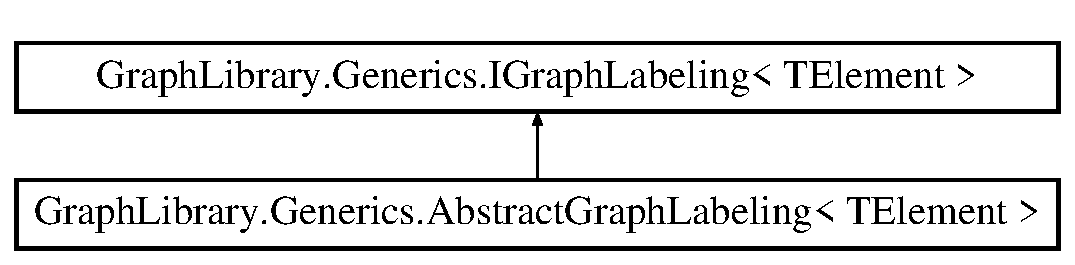
\includegraphics[height=2.000000cm]{class_graph_library_1_1_generics_1_1_abstract_graph_labeling}
\end{center}
\end{figure}
\subsection*{Public Member Functions}
\begin{DoxyCompactItemize}
\item 
virtual string \hyperlink{class_graph_library_1_1_generics_1_1_abstract_graph_labeling_ac9f80d3d85c1b5e0eb693bac9200e8ad}{Label} (T\+Element element)
\begin{DoxyCompactList}\small\item\em Returns the label of the given label. \end{DoxyCompactList}\item 
virtual string \hyperlink{class_graph_library_1_1_generics_1_1_abstract_graph_labeling_a1b94ec7d484a23a72a70ecc49f8058d4}{Label} (int serial\+Number)
\begin{DoxyCompactList}\small\item\em Returns label of the element with the specified serial\+Number. \end{DoxyCompactList}\item 
virtual T\+Element \hyperlink{class_graph_library_1_1_generics_1_1_abstract_graph_labeling_a3edd901c67ddc1ffbb54e0e35eb507dd}{Element} (string label)
\begin{DoxyCompactList}\small\item\em Returns the element that is labelled with the given label \end{DoxyCompactList}\item 
abstract void \hyperlink{class_graph_library_1_1_generics_1_1_abstract_graph_labeling_ad80b09ba50c168a12de02fd7936374ee}{Set\+Label} (T\+Element element, string label)
\begin{DoxyCompactList}\small\item\em Sets the label of the given element. The element must exist in the graph and the label must not be already used by another element of the same type (node, edge) The method is implemented in the concrete subclasses ( thats why is abstract because it depends on the graph class implementation ) \end{DoxyCompactList}\item 
abstract void \hyperlink{class_graph_library_1_1_generics_1_1_abstract_graph_labeling_a268a30e52ddd582947c6e35766627e73}{Set\+Label} (int serial\+Number, \hyperlink{namespace_graph_library_1_1_generics_a919a165f16deccdd1b3d7e8a93423fbc}{Graph\+Element\+Type} element\+Type, string label)
\begin{DoxyCompactList}\small\item\em Sets the label of the element with the given serialnumber and type. The element must exist in the graph and the label must not be already used by another element of the same type (node, edge) The method is implemented in the concrete subclasses ( thats why is abstract because it depends on the graph class implementation ) \end{DoxyCompactList}\end{DoxyCompactItemize}
\subsection*{Protected Member Functions}
\begin{DoxyCompactItemize}
\item 
abstract void \hyperlink{class_graph_library_1_1_generics_1_1_abstract_graph_labeling_a890775a0a91077bedd4330df8ddafe48}{Label\+Elements} ()
\begin{DoxyCompactList}\small\item\em Gives the initial mapping of labels to elements. Called by the constructor. Must be defined in subclasses \end{DoxyCompactList}\item 
virtual void \hyperlink{class_graph_library_1_1_generics_1_1_abstract_graph_labeling_a210863207176996b133a6d6c34d1c4a0}{Relabel\+Elements} ()
\begin{DoxyCompactList}\small\item\em Relabels the elements according to some algorithm. This version does nothing \end{DoxyCompactList}\end{DoxyCompactItemize}
\subsection*{Protected Attributes}
\begin{DoxyCompactItemize}
\item 
Dictionary$<$ T\+Element, string $>$ \hyperlink{class_graph_library_1_1_generics_1_1_abstract_graph_labeling_a6da5ad0ff86fe7cb0a33a0bf7ca9d27d}{m\+\_\+\+Labels\+Indexed\+By\+Elements}
\begin{DoxyCompactList}\small\item\em The mapping of elements to labels is represented by the dictionary variable m\+\_\+\+Element\+Labels \end{DoxyCompactList}\item 
Dictionary$<$ string, T\+Element $>$ \hyperlink{class_graph_library_1_1_generics_1_1_abstract_graph_labeling_a761265974897ab4d557e5896ab6df595}{m\+\_\+\+Elements\+Indexed\+By\+Labels}
\begin{DoxyCompactList}\small\item\em The mapping of labels to elements is represented by the dictionary variable \end{DoxyCompactList}\end{DoxyCompactItemize}


\subsection{Detailed Description}
This class holds the labels for a specific type of elements (edge , nodes, graphs ) of a graph. I use two dictionaries for both mapping to gain in query speed. This class gives the opportunity that diffrent graph clients can assign diffrent labels to the graph nodes, edges etc. The graph client ( contructor ) creates a subclass of \hyperlink{class_graph_library_1_1_generics_1_1_abstract_graph_labeling}{Abstract\+Graph\+Labeling$<$\+T$>$} and assigns labels to nodes. The instance of this class exists inside the \hyperlink{class_graph_library_1_1_c_graph}{C\+Graph} class and the client can add a new labeling of graph elements through the Add\+Graph\+Node\+Labelling() method. 


\begin{DoxyTemplParams}{Template Parameters}
{\em T\+Element} & Type of element to label\\
\hline
\end{DoxyTemplParams}
\begin{DoxySeeAlso}{See also}
I\+Graph\+Labeling$<$\+T$>$


\end{DoxySeeAlso}
\begin{Desc}
\item[Type Constraints]\begin{description}
\item[{\em T\+Element} : {\em \hyperlink{interface_graph_library_1_1_generics_1_1_i_graph_primitive}{I\+Graph\+Primitive}}]\end{description}
\end{Desc}


\subsection{Member Function Documentation}
\hypertarget{class_graph_library_1_1_generics_1_1_abstract_graph_labeling_a3edd901c67ddc1ffbb54e0e35eb507dd}{}\index{Graph\+Library\+::\+Generics\+::\+Abstract\+Graph\+Labeling@{Graph\+Library\+::\+Generics\+::\+Abstract\+Graph\+Labeling}!Element@{Element}}
\index{Element@{Element}!Graph\+Library\+::\+Generics\+::\+Abstract\+Graph\+Labeling@{Graph\+Library\+::\+Generics\+::\+Abstract\+Graph\+Labeling}}
\subsubsection[{Element(string label)}]{\setlength{\rightskip}{0pt plus 5cm}virtual T\+Element {\bf Graph\+Library.\+Generics.\+Abstract\+Graph\+Labeling}$<$ T\+Element $>$.Element (
\begin{DoxyParamCaption}
\item[{string}]{label}
\end{DoxyParamCaption}
)\hspace{0.3cm}{\ttfamily [virtual]}}\label{class_graph_library_1_1_generics_1_1_abstract_graph_labeling_a3edd901c67ddc1ffbb54e0e35eb507dd}


Returns the element that is labelled with the given label 


\begin{DoxyParams}{Parameters}
{\em label} & The label\\
\hline
\end{DoxyParams}
\begin{DoxyReturn}{Returns}
The element 
\end{DoxyReturn}

\begin{DoxyExceptions}{Exceptions}
{\em System.\+Collections.\+Generic.\+Key\+Not\+Found\+Exception} & \\
\hline
\end{DoxyExceptions}
\hypertarget{class_graph_library_1_1_generics_1_1_abstract_graph_labeling_ac9f80d3d85c1b5e0eb693bac9200e8ad}{}\index{Graph\+Library\+::\+Generics\+::\+Abstract\+Graph\+Labeling@{Graph\+Library\+::\+Generics\+::\+Abstract\+Graph\+Labeling}!Label@{Label}}
\index{Label@{Label}!Graph\+Library\+::\+Generics\+::\+Abstract\+Graph\+Labeling@{Graph\+Library\+::\+Generics\+::\+Abstract\+Graph\+Labeling}}
\subsubsection[{Label(\+T\+Element element)}]{\setlength{\rightskip}{0pt plus 5cm}virtual string {\bf Graph\+Library.\+Generics.\+Abstract\+Graph\+Labeling}$<$ T\+Element $>$.Label (
\begin{DoxyParamCaption}
\item[{T\+Element}]{element}
\end{DoxyParamCaption}
)\hspace{0.3cm}{\ttfamily [virtual]}}\label{class_graph_library_1_1_generics_1_1_abstract_graph_labeling_ac9f80d3d85c1b5e0eb693bac9200e8ad}


Returns the label of the given label. 


\begin{DoxyParams}{Parameters}
{\em element} & The labeled element\\
\hline
\end{DoxyParams}
\begin{DoxyReturn}{Returns}
The label 
\end{DoxyReturn}
\hypertarget{class_graph_library_1_1_generics_1_1_abstract_graph_labeling_a1b94ec7d484a23a72a70ecc49f8058d4}{}\index{Graph\+Library\+::\+Generics\+::\+Abstract\+Graph\+Labeling@{Graph\+Library\+::\+Generics\+::\+Abstract\+Graph\+Labeling}!Label@{Label}}
\index{Label@{Label}!Graph\+Library\+::\+Generics\+::\+Abstract\+Graph\+Labeling@{Graph\+Library\+::\+Generics\+::\+Abstract\+Graph\+Labeling}}
\subsubsection[{Label(int serial\+Number)}]{\setlength{\rightskip}{0pt plus 5cm}virtual string {\bf Graph\+Library.\+Generics.\+Abstract\+Graph\+Labeling}$<$ T\+Element $>$.Label (
\begin{DoxyParamCaption}
\item[{int}]{serial\+Number}
\end{DoxyParamCaption}
)\hspace{0.3cm}{\ttfamily [virtual]}}\label{class_graph_library_1_1_generics_1_1_abstract_graph_labeling_a1b94ec7d484a23a72a70ecc49f8058d4}


Returns label of the element with the specified serial\+Number. 


\begin{DoxyParams}{Parameters}
{\em serial\+Number} & The serial number of the labeled element\\
\hline
\end{DoxyParams}
\begin{DoxyReturn}{Returns}
The label 
\end{DoxyReturn}

\begin{DoxyExceptions}{Exceptions}
{\em System.\+Collections.\+Generic.\+Key\+Not\+Found\+Exception} & \\
\hline
\end{DoxyExceptions}
\hypertarget{class_graph_library_1_1_generics_1_1_abstract_graph_labeling_a890775a0a91077bedd4330df8ddafe48}{}\index{Graph\+Library\+::\+Generics\+::\+Abstract\+Graph\+Labeling@{Graph\+Library\+::\+Generics\+::\+Abstract\+Graph\+Labeling}!Label\+Elements@{Label\+Elements}}
\index{Label\+Elements@{Label\+Elements}!Graph\+Library\+::\+Generics\+::\+Abstract\+Graph\+Labeling@{Graph\+Library\+::\+Generics\+::\+Abstract\+Graph\+Labeling}}
\subsubsection[{Label\+Elements()}]{\setlength{\rightskip}{0pt plus 5cm}abstract void {\bf Graph\+Library.\+Generics.\+Abstract\+Graph\+Labeling}$<$ T\+Element $>$.Label\+Elements (
\begin{DoxyParamCaption}
{}
\end{DoxyParamCaption}
)\hspace{0.3cm}{\ttfamily [protected]}, {\ttfamily [pure virtual]}}\label{class_graph_library_1_1_generics_1_1_abstract_graph_labeling_a890775a0a91077bedd4330df8ddafe48}


Gives the initial mapping of labels to elements. Called by the constructor. Must be defined in subclasses 



Implemented in \hyperlink{class_graph_library_1_1_c_graph_labeling_aacfaf94dbe1fe9e65e95929a03d9f960}{Graph\+Library.\+C\+Graph\+Labeling$<$ T $>$}.

\hypertarget{class_graph_library_1_1_generics_1_1_abstract_graph_labeling_a210863207176996b133a6d6c34d1c4a0}{}\index{Graph\+Library\+::\+Generics\+::\+Abstract\+Graph\+Labeling@{Graph\+Library\+::\+Generics\+::\+Abstract\+Graph\+Labeling}!Relabel\+Elements@{Relabel\+Elements}}
\index{Relabel\+Elements@{Relabel\+Elements}!Graph\+Library\+::\+Generics\+::\+Abstract\+Graph\+Labeling@{Graph\+Library\+::\+Generics\+::\+Abstract\+Graph\+Labeling}}
\subsubsection[{Relabel\+Elements()}]{\setlength{\rightskip}{0pt plus 5cm}virtual void {\bf Graph\+Library.\+Generics.\+Abstract\+Graph\+Labeling}$<$ T\+Element $>$.Relabel\+Elements (
\begin{DoxyParamCaption}
{}
\end{DoxyParamCaption}
)\hspace{0.3cm}{\ttfamily [protected]}, {\ttfamily [virtual]}}\label{class_graph_library_1_1_generics_1_1_abstract_graph_labeling_a210863207176996b133a6d6c34d1c4a0}


Relabels the elements according to some algorithm. This version does nothing 

\hypertarget{class_graph_library_1_1_generics_1_1_abstract_graph_labeling_ad80b09ba50c168a12de02fd7936374ee}{}\index{Graph\+Library\+::\+Generics\+::\+Abstract\+Graph\+Labeling@{Graph\+Library\+::\+Generics\+::\+Abstract\+Graph\+Labeling}!Set\+Label@{Set\+Label}}
\index{Set\+Label@{Set\+Label}!Graph\+Library\+::\+Generics\+::\+Abstract\+Graph\+Labeling@{Graph\+Library\+::\+Generics\+::\+Abstract\+Graph\+Labeling}}
\subsubsection[{Set\+Label(\+T\+Element element, string label)}]{\setlength{\rightskip}{0pt plus 5cm}abstract void {\bf Graph\+Library.\+Generics.\+Abstract\+Graph\+Labeling}$<$ T\+Element $>$.Set\+Label (
\begin{DoxyParamCaption}
\item[{T\+Element}]{element, }
\item[{string}]{label}
\end{DoxyParamCaption}
)\hspace{0.3cm}{\ttfamily [pure virtual]}}\label{class_graph_library_1_1_generics_1_1_abstract_graph_labeling_ad80b09ba50c168a12de02fd7936374ee}


Sets the label of the given element. The element must exist in the graph and the label must not be already used by another element of the same type (node, edge) The method is implemented in the concrete subclasses ( thats why is abstract because it depends on the graph class implementation ) 


\begin{DoxyParams}{Parameters}
{\em element} & The element.\\
\hline
{\em label} & The label.\\
\hline
\end{DoxyParams}
\hypertarget{class_graph_library_1_1_generics_1_1_abstract_graph_labeling_a268a30e52ddd582947c6e35766627e73}{}\index{Graph\+Library\+::\+Generics\+::\+Abstract\+Graph\+Labeling@{Graph\+Library\+::\+Generics\+::\+Abstract\+Graph\+Labeling}!Set\+Label@{Set\+Label}}
\index{Set\+Label@{Set\+Label}!Graph\+Library\+::\+Generics\+::\+Abstract\+Graph\+Labeling@{Graph\+Library\+::\+Generics\+::\+Abstract\+Graph\+Labeling}}
\subsubsection[{Set\+Label(int serial\+Number, Graph\+Element\+Type element\+Type, string label)}]{\setlength{\rightskip}{0pt plus 5cm}abstract void {\bf Graph\+Library.\+Generics.\+Abstract\+Graph\+Labeling}$<$ T\+Element $>$.Set\+Label (
\begin{DoxyParamCaption}
\item[{int}]{serial\+Number, }
\item[{{\bf Graph\+Element\+Type}}]{element\+Type, }
\item[{string}]{label}
\end{DoxyParamCaption}
)\hspace{0.3cm}{\ttfamily [pure virtual]}}\label{class_graph_library_1_1_generics_1_1_abstract_graph_labeling_a268a30e52ddd582947c6e35766627e73}


Sets the label of the element with the given serialnumber and type. The element must exist in the graph and the label must not be already used by another element of the same type (node, edge) The method is implemented in the concrete subclasses ( thats why is abstract because it depends on the graph class implementation ) 


\begin{DoxyParams}{Parameters}
{\em serial\+Number} & The serial number.\\
\hline
{\em element\+Type} & Type of the element.\\
\hline
{\em label} & The label.\\
\hline
\end{DoxyParams}


Implemented in \hyperlink{class_graph_library_1_1_c_graph_labeling_abc0c9a99fd0ed7d21d3294c017587888}{Graph\+Library.\+C\+Graph\+Labeling$<$ T $>$}.



\subsection{Member Data Documentation}
\hypertarget{class_graph_library_1_1_generics_1_1_abstract_graph_labeling_a761265974897ab4d557e5896ab6df595}{}\index{Graph\+Library\+::\+Generics\+::\+Abstract\+Graph\+Labeling@{Graph\+Library\+::\+Generics\+::\+Abstract\+Graph\+Labeling}!m\+\_\+\+Elements\+Indexed\+By\+Labels@{m\+\_\+\+Elements\+Indexed\+By\+Labels}}
\index{m\+\_\+\+Elements\+Indexed\+By\+Labels@{m\+\_\+\+Elements\+Indexed\+By\+Labels}!Graph\+Library\+::\+Generics\+::\+Abstract\+Graph\+Labeling@{Graph\+Library\+::\+Generics\+::\+Abstract\+Graph\+Labeling}}
\subsubsection[{m\+\_\+\+Elements\+Indexed\+By\+Labels}]{\setlength{\rightskip}{0pt plus 5cm}Dictionary$<$string, T\+Element$>$ {\bf Graph\+Library.\+Generics.\+Abstract\+Graph\+Labeling}$<$ T\+Element $>$.m\+\_\+\+Elements\+Indexed\+By\+Labels\hspace{0.3cm}{\ttfamily [protected]}}\label{class_graph_library_1_1_generics_1_1_abstract_graph_labeling_a761265974897ab4d557e5896ab6df595}


The mapping of labels to elements is represented by the dictionary variable 

\hypertarget{class_graph_library_1_1_generics_1_1_abstract_graph_labeling_a6da5ad0ff86fe7cb0a33a0bf7ca9d27d}{}\index{Graph\+Library\+::\+Generics\+::\+Abstract\+Graph\+Labeling@{Graph\+Library\+::\+Generics\+::\+Abstract\+Graph\+Labeling}!m\+\_\+\+Labels\+Indexed\+By\+Elements@{m\+\_\+\+Labels\+Indexed\+By\+Elements}}
\index{m\+\_\+\+Labels\+Indexed\+By\+Elements@{m\+\_\+\+Labels\+Indexed\+By\+Elements}!Graph\+Library\+::\+Generics\+::\+Abstract\+Graph\+Labeling@{Graph\+Library\+::\+Generics\+::\+Abstract\+Graph\+Labeling}}
\subsubsection[{m\+\_\+\+Labels\+Indexed\+By\+Elements}]{\setlength{\rightskip}{0pt plus 5cm}Dictionary$<$T\+Element, string$>$ {\bf Graph\+Library.\+Generics.\+Abstract\+Graph\+Labeling}$<$ T\+Element $>$.m\+\_\+\+Labels\+Indexed\+By\+Elements\hspace{0.3cm}{\ttfamily [protected]}}\label{class_graph_library_1_1_generics_1_1_abstract_graph_labeling_a6da5ad0ff86fe7cb0a33a0bf7ca9d27d}


The mapping of elements to labels is represented by the dictionary variable m\+\_\+\+Element\+Labels 



The documentation for this class was generated from the following file\+:\begin{DoxyCompactItemize}
\item 
Graph\+Library/\+Generics/Abstract\+Graph\+Labeling.\+cs\end{DoxyCompactItemize}

\hypertarget{class_graph_library_1_1_generics_1_1_abstract_graph_printer}{}\section{Graph\+Library.\+Generics.\+Abstract\+Graph\+Printer$<$ T\+Graph $>$ Class Template Reference}
\label{class_graph_library_1_1_generics_1_1_abstract_graph_printer}\index{Graph\+Library.\+Generics.\+Abstract\+Graph\+Printer$<$ T\+Graph $>$@{Graph\+Library.\+Generics.\+Abstract\+Graph\+Printer$<$ T\+Graph $>$}}


This class is the parent class of all classes that print \hyperlink{class_graph_library_1_1_c_graph}{C\+Graph} objects Hence the class know the interface of \hyperlink{class_graph_library_1_1_c_graph}{C\+Graph}. (Its build for \hyperlink{class_graph_library_1_1_c_graph}{C\+Graph}). This class heirarchy is based on the Builder design pattern.  


\subsection*{Public Member Functions}
\begin{DoxyCompactItemize}
\item 
abstract String\+Builder \hyperlink{class_graph_library_1_1_generics_1_1_abstract_graph_printer_a793fd0ab2baf6809eee04292d3992ce4}{Print} (bool onlyedges=false)
\begin{DoxyCompactList}\small\item\em Prints the graph into a String\+Builder object \end{DoxyCompactList}\item 
abstract void \hyperlink{class_graph_library_1_1_generics_1_1_abstract_graph_printer_ae58857c9c21ef8ab2cd8a0651340e2ec}{Generate} (string filepath, bool execute\+Generator=true)
\begin{DoxyCompactList}\small\item\em Generates the graph representation to a file \end{DoxyCompactList}\end{DoxyCompactItemize}


\subsection{Detailed Description}
This class is the parent class of all classes that print \hyperlink{class_graph_library_1_1_c_graph}{C\+Graph} objects Hence the class know the interface of \hyperlink{class_graph_library_1_1_c_graph}{C\+Graph}. (Its build for \hyperlink{class_graph_library_1_1_c_graph}{C\+Graph}). This class heirarchy is based on the Builder design pattern. 



\subsection{Member Function Documentation}
\hypertarget{class_graph_library_1_1_generics_1_1_abstract_graph_printer_ae58857c9c21ef8ab2cd8a0651340e2ec}{}\index{Graph\+Library\+::\+Generics\+::\+Abstract\+Graph\+Printer@{Graph\+Library\+::\+Generics\+::\+Abstract\+Graph\+Printer}!Generate@{Generate}}
\index{Generate@{Generate}!Graph\+Library\+::\+Generics\+::\+Abstract\+Graph\+Printer@{Graph\+Library\+::\+Generics\+::\+Abstract\+Graph\+Printer}}
\subsubsection[{Generate(string filepath, bool execute\+Generator=true)}]{\setlength{\rightskip}{0pt plus 5cm}abstract void {\bf Graph\+Library.\+Generics.\+Abstract\+Graph\+Printer}$<$ T\+Graph $>$.Generate (
\begin{DoxyParamCaption}
\item[{string}]{filepath, }
\item[{bool}]{execute\+Generator = {\ttfamily true}}
\end{DoxyParamCaption}
)\hspace{0.3cm}{\ttfamily [pure virtual]}}\label{class_graph_library_1_1_generics_1_1_abstract_graph_printer_ae58857c9c21ef8ab2cd8a0651340e2ec}


Generates the graph representation to a file 



Implemented in \hyperlink{class_graph_library_1_1_c_graph_viz_printer_a9d4366ecf1b1f27c8886f0891ae5f5cf}{Graph\+Library.\+C\+Graph\+Viz\+Printer}.

\hypertarget{class_graph_library_1_1_generics_1_1_abstract_graph_printer_a793fd0ab2baf6809eee04292d3992ce4}{}\index{Graph\+Library\+::\+Generics\+::\+Abstract\+Graph\+Printer@{Graph\+Library\+::\+Generics\+::\+Abstract\+Graph\+Printer}!Print@{Print}}
\index{Print@{Print}!Graph\+Library\+::\+Generics\+::\+Abstract\+Graph\+Printer@{Graph\+Library\+::\+Generics\+::\+Abstract\+Graph\+Printer}}
\subsubsection[{Print(bool onlyedges=false)}]{\setlength{\rightskip}{0pt plus 5cm}abstract String\+Builder {\bf Graph\+Library.\+Generics.\+Abstract\+Graph\+Printer}$<$ T\+Graph $>$.Print (
\begin{DoxyParamCaption}
\item[{bool}]{onlyedges = {\ttfamily false}}
\end{DoxyParamCaption}
)\hspace{0.3cm}{\ttfamily [pure virtual]}}\label{class_graph_library_1_1_generics_1_1_abstract_graph_printer_a793fd0ab2baf6809eee04292d3992ce4}


Prints the graph into a String\+Builder object 


\begin{DoxyParams}{Parameters}
{\em onlyedges} & if set to {\ttfamily true} \mbox{[}onlyedges\mbox{]}.\\
\hline
\end{DoxyParams}
\begin{DoxyReturn}{Returns}

\end{DoxyReturn}


Implemented in \hyperlink{class_graph_library_1_1_c_graph_viz_printer_a5341d69647f313d81387578a629d1ed5}{Graph\+Library.\+C\+Graph\+Viz\+Printer}.



The documentation for this class was generated from the following file\+:\begin{DoxyCompactItemize}
\item 
Graph\+Library/\+Generics/Abstract\+Graph\+Printer.\+cs\end{DoxyCompactItemize}

\hypertarget{class_graph_library_1_1_generics_1_1_abstract_graph_query_info}{}\section{Graph\+Library.\+Generics.\+Abstract\+Graph\+Query\+Info$<$ Node, Edge, Graph $>$ Class Template Reference}
\label{class_graph_library_1_1_generics_1_1_abstract_graph_query_info}\index{Graph\+Library.\+Generics.\+Abstract\+Graph\+Query\+Info$<$ Node, Edge, Graph $>$@{Graph\+Library.\+Generics.\+Abstract\+Graph\+Query\+Info$<$ Node, Edge, Graph $>$}}


The purpose of this class is to simplify the expressions that the designer should write to access graph information from the code that describes the algorithm. This way the code that describes the algorithm is described with minimal complexity expressions something necessery to make him easily readapt to the code after long periods of abstention from this framework The class provides general access (takes object and returns object) to the node/edge information and requires casting to specialize it.  


\subsection*{Public Member Functions}
\begin{DoxyCompactItemize}
\item 
abstract object \hyperlink{class_graph_library_1_1_generics_1_1_abstract_graph_query_info_ac354a77c11aebe2f5fa87edadb9f05a1}{Info} (Node node, object key=null)
\begin{DoxyCompactList}\small\item\em Returns information concerning a node or a graph ( derives from node) Since the graph derives from \hyperlink{class_graph_library_1_1_c_graph_node}{C\+Graph\+Node} it stores the information at the same collection as node. So the function to retrieve the information is common in both elements \end{DoxyCompactList}\item 
abstract object \hyperlink{class_graph_library_1_1_generics_1_1_abstract_graph_query_info_a037261a2580a6f1946622de4f660e3b0}{Info} (Edge edge, object key=null)
\begin{DoxyCompactList}\small\item\em Returns the information of the specified edge \end{DoxyCompactList}\item 
abstract object \hyperlink{class_graph_library_1_1_generics_1_1_abstract_graph_query_info_a9a562930423ff0bca814ec0d13596134}{Info} (Node source, Node target, object key=null)
\begin{DoxyCompactList}\small\item\em Returns the information of the edge between the given source and target nodes. \end{DoxyCompactList}\item 
abstract object \hyperlink{class_graph_library_1_1_generics_1_1_abstract_graph_query_info_a58d00a825e3006b3066021fd992be858}{Create\+Info} (Node node, object info, object key=null)
\begin{DoxyCompactList}\small\item\em Stores the information at the specified node or graph. If information already exists, it is overwritten \end{DoxyCompactList}\item 
abstract object \hyperlink{class_graph_library_1_1_generics_1_1_abstract_graph_query_info_a39c8abaf3efbae750098bc6b0ed423da}{Create\+Info} (Edge edge, object info, object key=null)
\begin{DoxyCompactList}\small\item\em Stores the information at the specified edge. If information already exists, it is overwritten \end{DoxyCompactList}\item 
abstract object \hyperlink{class_graph_library_1_1_generics_1_1_abstract_graph_query_info_ad555b8fc4849bc003f0d457414edcb26}{Create\+Info} (Node source, Node target, object info, object key=null)
\begin{DoxyCompactList}\small\item\em Stores the information at the specified edge. If information already exists, it is overwritten \end{DoxyCompactList}\end{DoxyCompactItemize}
\subsection*{Protected Member Functions}
\begin{DoxyCompactItemize}
\item 
\hyperlink{class_graph_library_1_1_generics_1_1_abstract_graph_query_info_a8dd567e7f04df4a55df4bd8b4a0c3e48}{Abstract\+Graph\+Query\+Info} (Graph graph)
\begin{DoxyCompactList}\small\item\em Initializes a new instance of the \hyperlink{class_graph_library_1_1_generics_1_1_abstract_graph_query_info_a8dd567e7f04df4a55df4bd8b4a0c3e48}{Abstract\+Graph\+Query\+Info$<$\+Node, Edge, Graph$>$} class. \end{DoxyCompactList}\end{DoxyCompactItemize}
\subsection*{Protected Attributes}
\begin{DoxyCompactItemize}
\item 
Graph \hyperlink{class_graph_library_1_1_generics_1_1_abstract_graph_query_info_a7f1d5e09659d1e98da56197e1cc5973a}{m\+\_\+\+Graph}
\begin{DoxyCompactList}\small\item\em The graph to which the info refers \end{DoxyCompactList}\end{DoxyCompactItemize}


\subsection{Detailed Description}
The purpose of this class is to simplify the expressions that the designer should write to access graph information from the code that describes the algorithm. This way the code that describes the algorithm is described with minimal complexity expressions something necessery to make him easily readapt to the code after long periods of abstention from this framework The class provides general access (takes object and returns object) to the node/edge information and requires casting to specialize it. 


\begin{DoxyTemplParams}{Template Parameters}
{\em Node} & The type of the node.\\
\hline
{\em Edge} & The type of the edge.\\
\hline
{\em Graph} & The type of the graph.\\
\hline
\end{DoxyTemplParams}


\subsection{Constructor \& Destructor Documentation}
\hypertarget{class_graph_library_1_1_generics_1_1_abstract_graph_query_info_a8dd567e7f04df4a55df4bd8b4a0c3e48}{}\index{Graph\+Library\+::\+Generics\+::\+Abstract\+Graph\+Query\+Info@{Graph\+Library\+::\+Generics\+::\+Abstract\+Graph\+Query\+Info}!Abstract\+Graph\+Query\+Info@{Abstract\+Graph\+Query\+Info}}
\index{Abstract\+Graph\+Query\+Info@{Abstract\+Graph\+Query\+Info}!Graph\+Library\+::\+Generics\+::\+Abstract\+Graph\+Query\+Info@{Graph\+Library\+::\+Generics\+::\+Abstract\+Graph\+Query\+Info}}
\subsubsection[{Abstract\+Graph\+Query\+Info(\+Graph graph)}]{\setlength{\rightskip}{0pt plus 5cm}{\bf Graph\+Library.\+Generics.\+Abstract\+Graph\+Query\+Info}$<$ Node, Edge, Graph $>$.{\bf Abstract\+Graph\+Query\+Info} (
\begin{DoxyParamCaption}
\item[{Graph}]{graph}
\end{DoxyParamCaption}
)\hspace{0.3cm}{\ttfamily [protected]}}\label{class_graph_library_1_1_generics_1_1_abstract_graph_query_info_a8dd567e7f04df4a55df4bd8b4a0c3e48}


Initializes a new instance of the \hyperlink{class_graph_library_1_1_generics_1_1_abstract_graph_query_info_a8dd567e7f04df4a55df4bd8b4a0c3e48}{Abstract\+Graph\+Query\+Info$<$\+Node, Edge, Graph$>$} class. 


\begin{DoxyParams}{Parameters}
{\em graph} & The graph.\\
\hline
\end{DoxyParams}


\subsection{Member Function Documentation}
\hypertarget{class_graph_library_1_1_generics_1_1_abstract_graph_query_info_a58d00a825e3006b3066021fd992be858}{}\index{Graph\+Library\+::\+Generics\+::\+Abstract\+Graph\+Query\+Info@{Graph\+Library\+::\+Generics\+::\+Abstract\+Graph\+Query\+Info}!Create\+Info@{Create\+Info}}
\index{Create\+Info@{Create\+Info}!Graph\+Library\+::\+Generics\+::\+Abstract\+Graph\+Query\+Info@{Graph\+Library\+::\+Generics\+::\+Abstract\+Graph\+Query\+Info}}
\subsubsection[{Create\+Info(\+Node node, object info, object key=null)}]{\setlength{\rightskip}{0pt plus 5cm}abstract object {\bf Graph\+Library.\+Generics.\+Abstract\+Graph\+Query\+Info}$<$ Node, Edge, Graph $>$.Create\+Info (
\begin{DoxyParamCaption}
\item[{Node}]{node, }
\item[{object}]{info, }
\item[{object}]{key = {\ttfamily null}}
\end{DoxyParamCaption}
)\hspace{0.3cm}{\ttfamily [pure virtual]}}\label{class_graph_library_1_1_generics_1_1_abstract_graph_query_info_a58d00a825e3006b3066021fd992be858}


Stores the information at the specified node or graph. If information already exists, it is overwritten 


\begin{DoxyParams}{Parameters}
{\em node} & The node.\\
\hline
{\em info} & The information object\\
\hline
{\em key} & The key that will extract the information from the specified node\textquotesingle{}s dictionary\\
\hline
\end{DoxyParams}
\begin{DoxyReturn}{Returns}
The information object
\end{DoxyReturn}
\hypertarget{class_graph_library_1_1_generics_1_1_abstract_graph_query_info_a39c8abaf3efbae750098bc6b0ed423da}{}\index{Graph\+Library\+::\+Generics\+::\+Abstract\+Graph\+Query\+Info@{Graph\+Library\+::\+Generics\+::\+Abstract\+Graph\+Query\+Info}!Create\+Info@{Create\+Info}}
\index{Create\+Info@{Create\+Info}!Graph\+Library\+::\+Generics\+::\+Abstract\+Graph\+Query\+Info@{Graph\+Library\+::\+Generics\+::\+Abstract\+Graph\+Query\+Info}}
\subsubsection[{Create\+Info(\+Edge edge, object info, object key=null)}]{\setlength{\rightskip}{0pt plus 5cm}abstract object {\bf Graph\+Library.\+Generics.\+Abstract\+Graph\+Query\+Info}$<$ Node, Edge, Graph $>$.Create\+Info (
\begin{DoxyParamCaption}
\item[{Edge}]{edge, }
\item[{object}]{info, }
\item[{object}]{key = {\ttfamily null}}
\end{DoxyParamCaption}
)\hspace{0.3cm}{\ttfamily [pure virtual]}}\label{class_graph_library_1_1_generics_1_1_abstract_graph_query_info_a39c8abaf3efbae750098bc6b0ed423da}


Stores the information at the specified edge. If information already exists, it is overwritten 


\begin{DoxyParams}{Parameters}
{\em edge} & The edge.\\
\hline
{\em info} & The information object\\
\hline
{\em key} & The key that will extract the information from the specified edge\textquotesingle{}s dictionary\\
\hline
\end{DoxyParams}
\begin{DoxyReturn}{Returns}
The information object
\end{DoxyReturn}
\hypertarget{class_graph_library_1_1_generics_1_1_abstract_graph_query_info_ad555b8fc4849bc003f0d457414edcb26}{}\index{Graph\+Library\+::\+Generics\+::\+Abstract\+Graph\+Query\+Info@{Graph\+Library\+::\+Generics\+::\+Abstract\+Graph\+Query\+Info}!Create\+Info@{Create\+Info}}
\index{Create\+Info@{Create\+Info}!Graph\+Library\+::\+Generics\+::\+Abstract\+Graph\+Query\+Info@{Graph\+Library\+::\+Generics\+::\+Abstract\+Graph\+Query\+Info}}
\subsubsection[{Create\+Info(\+Node source, Node target, object info, object key=null)}]{\setlength{\rightskip}{0pt plus 5cm}abstract object {\bf Graph\+Library.\+Generics.\+Abstract\+Graph\+Query\+Info}$<$ Node, Edge, Graph $>$.Create\+Info (
\begin{DoxyParamCaption}
\item[{Node}]{source, }
\item[{Node}]{target, }
\item[{object}]{info, }
\item[{object}]{key = {\ttfamily null}}
\end{DoxyParamCaption}
)\hspace{0.3cm}{\ttfamily [pure virtual]}}\label{class_graph_library_1_1_generics_1_1_abstract_graph_query_info_ad555b8fc4849bc003f0d457414edcb26}


Stores the information at the specified edge. If information already exists, it is overwritten 


\begin{DoxyParams}{Parameters}
{\em source} & The source node.\\
\hline
{\em target} & The target node.\\
\hline
{\em info} & The information object\\
\hline
{\em key} & The key that will extract the information from the specified edge\textquotesingle{}s dictionary\\
\hline
\end{DoxyParams}
\begin{DoxyReturn}{Returns}
The information object
\end{DoxyReturn}
\hypertarget{class_graph_library_1_1_generics_1_1_abstract_graph_query_info_ac354a77c11aebe2f5fa87edadb9f05a1}{}\index{Graph\+Library\+::\+Generics\+::\+Abstract\+Graph\+Query\+Info@{Graph\+Library\+::\+Generics\+::\+Abstract\+Graph\+Query\+Info}!Info@{Info}}
\index{Info@{Info}!Graph\+Library\+::\+Generics\+::\+Abstract\+Graph\+Query\+Info@{Graph\+Library\+::\+Generics\+::\+Abstract\+Graph\+Query\+Info}}
\subsubsection[{Info(\+Node node, object key=null)}]{\setlength{\rightskip}{0pt plus 5cm}abstract object {\bf Graph\+Library.\+Generics.\+Abstract\+Graph\+Query\+Info}$<$ Node, Edge, Graph $>$.Info (
\begin{DoxyParamCaption}
\item[{Node}]{node, }
\item[{object}]{key = {\ttfamily null}}
\end{DoxyParamCaption}
)\hspace{0.3cm}{\ttfamily [pure virtual]}}\label{class_graph_library_1_1_generics_1_1_abstract_graph_query_info_ac354a77c11aebe2f5fa87edadb9f05a1}


Returns information concerning a node or a graph ( derives from node) Since the graph derives from \hyperlink{class_graph_library_1_1_c_graph_node}{C\+Graph\+Node} it stores the information at the same collection as node. So the function to retrieve the information is common in both elements 


\begin{DoxyParams}{Parameters}
{\em node} & The node.\\
\hline
{\em key} & The key that will extract the information from the specified node\textquotesingle{}s dictionary\\
\hline
\end{DoxyParams}
\begin{DoxyReturn}{Returns}

\end{DoxyReturn}
\hypertarget{class_graph_library_1_1_generics_1_1_abstract_graph_query_info_a037261a2580a6f1946622de4f660e3b0}{}\index{Graph\+Library\+::\+Generics\+::\+Abstract\+Graph\+Query\+Info@{Graph\+Library\+::\+Generics\+::\+Abstract\+Graph\+Query\+Info}!Info@{Info}}
\index{Info@{Info}!Graph\+Library\+::\+Generics\+::\+Abstract\+Graph\+Query\+Info@{Graph\+Library\+::\+Generics\+::\+Abstract\+Graph\+Query\+Info}}
\subsubsection[{Info(\+Edge edge, object key=null)}]{\setlength{\rightskip}{0pt plus 5cm}abstract object {\bf Graph\+Library.\+Generics.\+Abstract\+Graph\+Query\+Info}$<$ Node, Edge, Graph $>$.Info (
\begin{DoxyParamCaption}
\item[{Edge}]{edge, }
\item[{object}]{key = {\ttfamily null}}
\end{DoxyParamCaption}
)\hspace{0.3cm}{\ttfamily [pure virtual]}}\label{class_graph_library_1_1_generics_1_1_abstract_graph_query_info_a037261a2580a6f1946622de4f660e3b0}


Returns the information of the specified edge 


\begin{DoxyParams}{Parameters}
{\em edge} & The edge.\\
\hline
{\em key} & The key that will extract the information from the specified edge\textquotesingle{}s dictionary\\
\hline
\end{DoxyParams}
\begin{DoxyReturn}{Returns}

\end{DoxyReturn}
\hypertarget{class_graph_library_1_1_generics_1_1_abstract_graph_query_info_a9a562930423ff0bca814ec0d13596134}{}\index{Graph\+Library\+::\+Generics\+::\+Abstract\+Graph\+Query\+Info@{Graph\+Library\+::\+Generics\+::\+Abstract\+Graph\+Query\+Info}!Info@{Info}}
\index{Info@{Info}!Graph\+Library\+::\+Generics\+::\+Abstract\+Graph\+Query\+Info@{Graph\+Library\+::\+Generics\+::\+Abstract\+Graph\+Query\+Info}}
\subsubsection[{Info(\+Node source, Node target, object key=null)}]{\setlength{\rightskip}{0pt plus 5cm}abstract object {\bf Graph\+Library.\+Generics.\+Abstract\+Graph\+Query\+Info}$<$ Node, Edge, Graph $>$.Info (
\begin{DoxyParamCaption}
\item[{Node}]{source, }
\item[{Node}]{target, }
\item[{object}]{key = {\ttfamily null}}
\end{DoxyParamCaption}
)\hspace{0.3cm}{\ttfamily [pure virtual]}}\label{class_graph_library_1_1_generics_1_1_abstract_graph_query_info_a9a562930423ff0bca814ec0d13596134}


Returns the information of the edge between the given source and target nodes. 


\begin{DoxyParams}{Parameters}
{\em source} & The source.\\
\hline
{\em target} & The target.\\
\hline
{\em key} & The key that will extract the information from the specified edge\textquotesingle{}s dictionary\\
\hline
\end{DoxyParams}
\begin{DoxyReturn}{Returns}

\end{DoxyReturn}


\subsection{Member Data Documentation}
\hypertarget{class_graph_library_1_1_generics_1_1_abstract_graph_query_info_a7f1d5e09659d1e98da56197e1cc5973a}{}\index{Graph\+Library\+::\+Generics\+::\+Abstract\+Graph\+Query\+Info@{Graph\+Library\+::\+Generics\+::\+Abstract\+Graph\+Query\+Info}!m\+\_\+\+Graph@{m\+\_\+\+Graph}}
\index{m\+\_\+\+Graph@{m\+\_\+\+Graph}!Graph\+Library\+::\+Generics\+::\+Abstract\+Graph\+Query\+Info@{Graph\+Library\+::\+Generics\+::\+Abstract\+Graph\+Query\+Info}}
\subsubsection[{m\+\_\+\+Graph}]{\setlength{\rightskip}{0pt plus 5cm}Graph {\bf Graph\+Library.\+Generics.\+Abstract\+Graph\+Query\+Info}$<$ Node, Edge, Graph $>$.m\+\_\+\+Graph\hspace{0.3cm}{\ttfamily [protected]}}\label{class_graph_library_1_1_generics_1_1_abstract_graph_query_info_a7f1d5e09659d1e98da56197e1cc5973a}


The graph to which the info refers 



The documentation for this class was generated from the following file\+:\begin{DoxyCompactItemize}
\item 
Graph\+Library/\+Generics/Abstract\+Query\+Info.\+cs\end{DoxyCompactItemize}

\hypertarget{class_graph_library_1_1_c_graph}{}\section{Graph\+Library.\+C\+Graph Class Reference}
\label{class_graph_library_1_1_c_graph}\index{Graph\+Library.\+C\+Graph@{Graph\+Library.\+C\+Graph}}


The Graph holds the list of nodes and the list of edges as well as the type of graph ( directed / undirected )  


Inheritance diagram for Graph\+Library.\+C\+Graph\+:\begin{figure}[H]
\begin{center}
\leavevmode
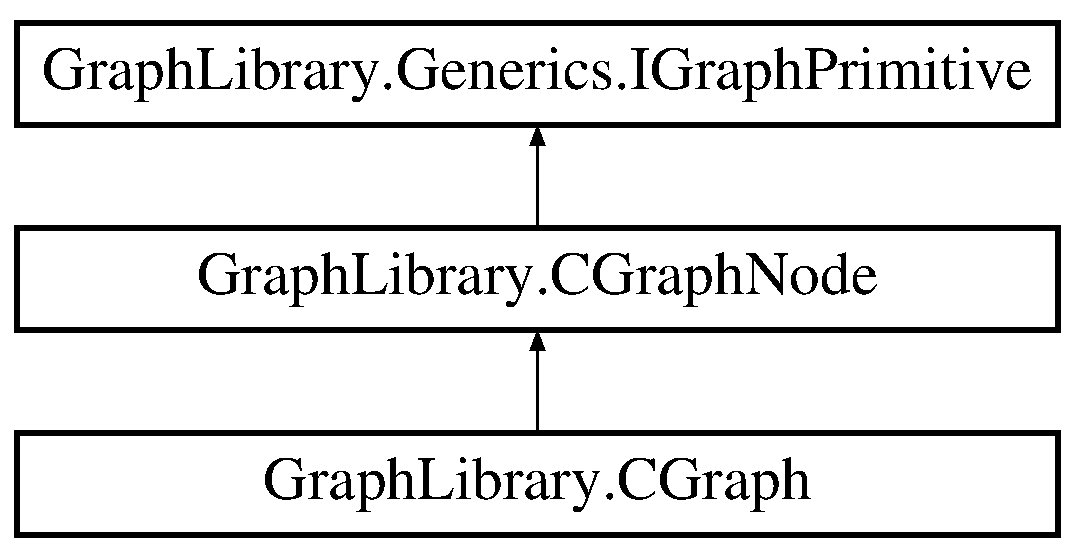
\includegraphics[height=3.000000cm]{class_graph_library_1_1_c_graph}
\end{center}
\end{figure}
\subsection*{Public Member Functions}
\begin{DoxyCompactItemize}
\item 
\hyperlink{class_graph_library_1_1_c_graph_node}{C\+Graph\+Node} \hyperlink{class_graph_library_1_1_c_graph_aaf1c7e3fc443585374700fdcb71f0289}{Create\+Graph\+Node} ()
\begin{DoxyCompactList}\small\item\em Creates and adds a node to the graph. Gives the default label, the node\textquotesingle{}s serialnumber \end{DoxyCompactList}\item 
\hyperlink{class_graph_library_1_1_c_graph_node}{C\+Graph\+Node} \hyperlink{class_graph_library_1_1_c_graph_af60c41b8fe601277ec6bb45fcb2768a7}{Create\+Graph\+Node} (string label)
\begin{DoxyCompactList}\small\item\em Creates the graph node and gives it the specified label \end{DoxyCompactList}\item 
void \hyperlink{class_graph_library_1_1_c_graph_a299d93f0be8ed93b1e17817c6f5bf5cc}{Add\+Graph\+Node} (\hyperlink{class_graph_library_1_1_c_graph_node}{C\+Graph\+Node} newnode)
\begin{DoxyCompactList}\small\item\em Adds an existing node to the graph. Assumes that the node does not already belong to another graph \end{DoxyCompactList}\item 
void \hyperlink{class_graph_library_1_1_c_graph_ae7eafc40d87100bf02a189a502ec6881}{Add\+Graph\+Node\+Labelling} (object labels\+Contructor, \hyperlink{class_graph_library_1_1_c_graph_labeling}{C\+Graph\+Labeling}$<$ \hyperlink{class_graph_library_1_1_c_graph_node}{C\+Graph\+Node} $>$ nodelabeling)
\begin{DoxyCompactList}\small\item\em Adds the graph node labelling Contructor. \end{DoxyCompactList}\item 
void \hyperlink{class_graph_library_1_1_c_graph_a44eca07849f3cbb2f28db1fcae27802f}{Add\+Graph\+Edge\+Labelling} (object labels\+Contructor, \hyperlink{class_graph_library_1_1_c_graph_labeling}{C\+Graph\+Labeling}$<$ \hyperlink{class_graph_library_1_1_c_graph_edge}{C\+Graph\+Edge} $>$ edgelabeling)
\begin{DoxyCompactList}\small\item\em Adds the graph edge labelling. \end{DoxyCompactList}\item 
string \hyperlink{class_graph_library_1_1_c_graph_a84eb3418b6dca4fc1d8dea9d1864493d}{Node\+Label} (object label\+Contructor, \hyperlink{class_graph_library_1_1_c_graph_node}{C\+Graph\+Node} node)
\begin{DoxyCompactList}\small\item\em Returns a node label given for a specified contructor ( algorithm ,printer etc) \end{DoxyCompactList}\item 
string \hyperlink{class_graph_library_1_1_c_graph_a31064cccadfc56bb1d4bcb9a1605ad27}{Node\+Label} (object label\+Contructor, int serial\+Number)
\begin{DoxyCompactList}\small\item\em Returns a node label given for a specified contructor ( algorithm ,printer etc) \end{DoxyCompactList}\item 
void \hyperlink{class_graph_library_1_1_c_graph_a670c9a24d5244887e9c231707c7eef57}{Set\+Node\+Label} (\hyperlink{class_graph_library_1_1_c_graph_node}{C\+Graph\+Node} node, string label)
\begin{DoxyCompactList}\small\item\em Sets the label of the specified node using the host graph as label contructor. \end{DoxyCompactList}\item 
void \hyperlink{class_graph_library_1_1_c_graph_a3ef7f744ad2a374e1fa7eeded40325e4}{Set\+Edge\+Label} (\hyperlink{class_graph_library_1_1_c_graph_edge}{C\+Graph\+Edge} edge, string label)
\begin{DoxyCompactList}\small\item\em Sets the label of the specified edge for using the host graph as label contructor. \end{DoxyCompactList}\item 
\hyperlink{class_graph_library_1_1_c_graph_edge}{C\+Graph\+Edge} \hyperlink{class_graph_library_1_1_c_graph_af12db1b8e252d2a1e3179d12180798dc}{Add\+Graph\+Edge} (\hyperlink{class_graph_library_1_1_c_graph_node}{C\+Graph\+Node} source, \hyperlink{class_graph_library_1_1_c_graph_node}{C\+Graph\+Node} target, \hyperlink{namespace_graph_library_1_1_generics_a1bac729ea88e6f3925406df33f15d056}{Graph\+Type} edgetype=Graph\+Type.\+G\+T\+\_\+\+D\+I\+R\+E\+C\+T\+E\+D)
\begin{DoxyCompactList}\small\item\em Adds a native edge to the graph and label it with the default ie its serialnumber. N\+O\+T\+I\+C\+E\+: If you want to add a foreign edge do it through \hyperlink{class_graph_library_1_1_c_graph}{C\+Graph} object containing both the source and the target node. An edge that connects nodes of diffrent graphs does not belong to any of these graphs but at the graph that contain\textquotesingle{}s them \end{DoxyCompactList}\item 
\hyperlink{class_graph_library_1_1_c_graph_edge}{C\+Graph\+Edge} \hyperlink{class_graph_library_1_1_c_graph_af57fff06c0780defe3574dbe22c51902}{Add\+Graph\+Edge} (\hyperlink{class_graph_library_1_1_c_graph_node}{C\+Graph\+Node} source, \hyperlink{class_graph_library_1_1_c_graph_node}{C\+Graph\+Node} target, string label, \hyperlink{namespace_graph_library_1_1_generics_a1bac729ea88e6f3925406df33f15d056}{Graph\+Type} edgetype=Graph\+Type.\+G\+T\+\_\+\+D\+I\+R\+E\+C\+T\+E\+D)
\begin{DoxyCompactList}\small\item\em Adds a native edge to the graph with the given label. N\+O\+T\+I\+C\+E\+: If you want to add a foreign edge do it through \hyperlink{class_graph_library_1_1_c_graph}{C\+Graph} object containing both the source and the target node. An edge that connects nodes of diffrent graphs does not belong to any of these graphs but at the graph that contain\textquotesingle{}s them \end{DoxyCompactList}\item 
void \hyperlink{class_graph_library_1_1_c_graph_a572ac323b5642ac9ba3a8755748b3f5e}{Remove\+Node} (\hyperlink{class_graph_library_1_1_c_graph_node}{C\+Graph\+Node} node)
\begin{DoxyCompactList}\small\item\em Removes a node from the graph. \end{DoxyCompactList}\item 
void \hyperlink{class_graph_library_1_1_c_graph_a3e02229a24c28d1ebbf3ec5f12d1a145}{Remove\+Native\+Graph\+Edge} (\hyperlink{class_graph_library_1_1_c_graph_edge}{C\+Graph\+Edge} edge)
\begin{DoxyCompactList}\small\item\em Deletes a native graph edge. \end{DoxyCompactList}\item 
\hyperlink{class_graph_library_1_1_c_graph_node}{C\+Graph\+Node} \hyperlink{class_graph_library_1_1_c_graph_a93fba5a60f4cec728a6511049bc7c079}{Node} (int index)
\begin{DoxyCompactList}\small\item\em Returns a node at the specified index or raises an exception when a non existing node is indexed \end{DoxyCompactList}\item 
\hyperlink{namespace_graph_library_1_1_generics_a919a165f16deccdd1b3d7e8a93423fbc}{Graph\+Element\+Type} \hyperlink{class_graph_library_1_1_c_graph_a11e37ac22c8c9770a53ef80e54c7adfa}{Contains} (\hyperlink{interface_graph_library_1_1_generics_1_1_i_graph_primitive}{I\+Graph\+Primitive} element)
\begin{DoxyCompactList}\small\item\em Determines whether the graph contains the specified element \end{DoxyCompactList}\item 
\hyperlink{interface_graph_library_1_1_generics_1_1_i_graph_primitive}{I\+Graph\+Primitive} \hyperlink{class_graph_library_1_1_c_graph_aafdb175ad7467a414d37eecac0ea05d1}{Contains} (int serial\+Number, \hyperlink{namespace_graph_library_1_1_generics_a919a165f16deccdd1b3d7e8a93423fbc}{Graph\+Element\+Type} element\+Type)
\begin{DoxyCompactList}\small\item\em Determines whether the element with the given serial number and type exists in the graph \end{DoxyCompactList}\item 
\hyperlink{class_graph_library_1_1_c_graph_node}{C\+Graph\+Node} \hyperlink{class_graph_library_1_1_c_graph_a6a468edc9fb6a205ddbe5e8de847a745}{Node} (string label, object label\+Context\+Key)
\begin{DoxyCompactList}\small\item\em Returns the node with the given label from the given label context. Different contexts may assign different labels to the nodes. By default a node is labelled only by its serialnumber which is unique. In the default case call public \hyperlink{class_graph_library_1_1_c_graph_node}{C\+Graph\+Node} \hyperlink{class_graph_library_1_1_c_graph_a93fba5a60f4cec728a6511049bc7c079}{Node(int index)} method \end{DoxyCompactList}\item 
\hyperlink{class_graph_library_1_1_c_graph_edge}{C\+Graph\+Edge} \hyperlink{class_graph_library_1_1_c_graph_aed4132c7cc61ce43d85a3cde3b6334af}{Edge} (string label, object label\+Context\+Key)
\begin{DoxyCompactList}\small\item\em Returns the edge with the given label from the given label context. Different contexts may assign different labels to the edges. By default a edge is labelled only by its serialnumber which is unique. In the default case call public \hyperlink{class_graph_library_1_1_c_graph_edge}{C\+Graph\+Edge} \hyperlink{class_graph_library_1_1_c_graph_a0aa4b87cbe9c0c8f9956ebc9d45f11f8}{Edge(int source, int target)} method \end{DoxyCompactList}\item 
\hyperlink{class_graph_library_1_1_c_graph_edge}{C\+Graph\+Edge} \hyperlink{class_graph_library_1_1_c_graph_a0aa4b87cbe9c0c8f9956ebc9d45f11f8}{Edge} (int source, int target)
\begin{DoxyCompactList}\small\item\em Returns the N\+A\+T\+I\+V\+E edge between the source and the target nodes. It returns the first edge it finds with the specified source and sink. If parallel edges are supported use the function Edges that returns a list of edges having the same source and target nodes. The function returns null if it doesn\textquotesingle{}t find the edge. \end{DoxyCompactList}\item 
\hyperlink{class_graph_library_1_1_c_graph_edge}{C\+Graph\+Edge} \hyperlink{class_graph_library_1_1_c_graph_a9a1acc1f91a1d8de411ee77d3826f996}{Edge} (\hyperlink{class_graph_library_1_1_c_graph_node}{C\+Graph\+Node} source, \hyperlink{class_graph_library_1_1_c_graph_node}{C\+Graph\+Node} target)
\begin{DoxyCompactList}\small\item\em Returns the N\+A\+T\+I\+V\+E edge between the source and the target nodes. It returns the first edge it finds with the specified source and sink. If parallel edges are supported use the function Edges that returns a list of edges having the same source and target nodes. The function returns null if it doesn\textquotesingle{}t find the edge. \end{DoxyCompactList}\item 
List$<$ \hyperlink{class_graph_library_1_1_c_graph_edge}{C\+Graph\+Edge} $>$ \hyperlink{class_graph_library_1_1_c_graph_a06c8ee25ece0294e50501796a1c22dd9}{Edges} (int source, int target)
\begin{DoxyCompactList}\small\item\em Returns all the edges it finds between the source and target nodes. In case where the graph doesn\textquotesingle{}t have parallel edges its preferable tha you call the Edge function. The edges are return in a list or null if no edge were found between the specified source and sink node \end{DoxyCompactList}\item 
void \hyperlink{class_graph_library_1_1_c_graph_a1585ebb9c26742a09b342a67a066e9ee}{Generate\+Graph\+\_\+\+Random\+Edges} (int Num\+Vertices, int Num\+Edges, \hyperlink{namespace_graph_library_1_1_generics_a1bac729ea88e6f3925406df33f15d056}{Graph\+Type} graphtype=Graph\+Type.\+G\+T\+\_\+\+D\+I\+R\+E\+C\+T\+E\+D, bool loops=false, bool paralleledges=false)
\begin{DoxyCompactList}\small\item\em Creates a random graph of the given type and number of nodes and edges. The method creates Num\+Vertices and creates Num\+Edges random edges between them. This function is made according to the algorithm Program 17.\+12 Random graph generator (random edges) in the book Graph Algorithms Sedgewick 2002 Notice that the final number of edges inserted to the graph is smaller or equal to the requested number because some edges might be excluded due to the two switches loops and paralleledges. Assumes that the graph is empty \end{DoxyCompactList}\item 
void \hyperlink{class_graph_library_1_1_c_graph_aec37e426c9745454988e8c4e75ac8b1d}{Generate\+Graph\+\_\+\+Random\+Graph} (int Num\+Vertices, int Num\+Edges, \hyperlink{namespace_graph_library_1_1_generics_a1bac729ea88e6f3925406df33f15d056}{Graph\+Type} graphtype=Graph\+Type.\+G\+T\+\_\+\+D\+I\+R\+E\+C\+T\+E\+D, bool loops=false, bool paralleledges=false)
\begin{DoxyCompactList}\small\item\em Creates a random graph with the given number of vertices. The algorithm considers every possible pair of nodes and draws an edge between them based on some probability that can be defined by the designer. The main characteristic of this algorithm is that all pairs of nodes are considered however not all possible edges are drawn. This gives the possibility to draw graphs that the edges exhibit some properties ( i.\+e locality \+: connect mostly nearby nodes etc ) In a directed graph Parallel edges cannot exist because its pair is considered once Assumes that the graph is empty \end{DoxyCompactList}\item 
void \hyperlink{class_graph_library_1_1_c_graph_ae9e690d0f3b0b84f837de51a08550f51}{Generate} (string filepath, bool execute\+Generator=true)
\begin{DoxyCompactList}\small\item\em Calls the tool that renders the graph to some representable media \end{DoxyCompactList}\item 
void \hyperlink{class_graph_library_1_1_c_graph_a441e3e9293be54f3a8503fdc655d59d9}{Register\+Graph\+Printer} (\hyperlink{class_graph_library_1_1_c_graph_printer}{C\+Graph\+Printer} printer)
\begin{DoxyCompactList}\small\item\em Registers a printer to the graph. The printer is added if it doesn\textquotesingle{}t already exists and if it is not null \end{DoxyCompactList}\end{DoxyCompactItemize}
\subsection*{Static Public Member Functions}
\begin{DoxyCompactItemize}
\item 
static \hyperlink{class_graph_library_1_1_c_graph}{C\+Graph} \hyperlink{class_graph_library_1_1_c_graph_af4914521623ddb668b21285684e6e6fc}{Create\+Graph} (\hyperlink{class_graph_library_1_1_c_graph}{C\+Graph} owner\+Graph=null)
\begin{DoxyCompactList}\small\item\em Creates a new graph. The \hyperlink{class_graph_library_1_1_c_graph}{C\+Graph} constructor is protected and hence this method acts as a constructor. ownergraph parameter is null only this function creates the top level graph. If the ownergraph is not null the graph is labelled with the default ie. its serialnumber \end{DoxyCompactList}\item 
static \hyperlink{class_graph_library_1_1_c_graph}{C\+Graph} \hyperlink{class_graph_library_1_1_c_graph_a4e157e57dd1a6c927935c27d3e16fd00}{Create\+Graph\+From\+C\+S\+V} (string filename, \hyperlink{class_graph_library_1_1_c_graph}{C\+Graph} owner\+Graph=null)
\begin{DoxyCompactList}\small\item\em Creates the graph from C\+S\+V file. \end{DoxyCompactList}\end{DoxyCompactItemize}
\subsection*{Protected Member Functions}
\begin{DoxyCompactItemize}
\item 
\hyperlink{class_graph_library_1_1_c_graph_a62d8da6f4b059adea3ef77ea8e014569}{C\+Graph} (\hyperlink{class_graph_library_1_1_c_graph}{C\+Graph} owner\+Graph)
\begin{DoxyCompactList}\small\item\em Initializes a new instance of the \hyperlink{class_graph_library_1_1_c_graph}{C\+Graph} class. \end{DoxyCompactList}\end{DoxyCompactItemize}
\subsection*{Protected Attributes}
\begin{DoxyCompactItemize}
\item 
List$<$ \hyperlink{class_graph_library_1_1_c_graph_node}{C\+Graph\+Node} $>$ \hyperlink{class_graph_library_1_1_c_graph_abccc3feed7b02988f555743364ea4ea8}{m\+\_\+graph\+Nodes}
\begin{DoxyCompactList}\small\item\em List of graph nodes \end{DoxyCompactList}\item 
List$<$ \hyperlink{class_graph_library_1_1_c_graph_edge}{C\+Graph\+Edge} $>$ \hyperlink{class_graph_library_1_1_c_graph_af16b65e1c7b51ba0f3be2d5fb4ab67b4}{m\+\_\+graph\+Edges}
\begin{DoxyCompactList}\small\item\em List of graph\textquotesingle{}s native edges. All the edges of a graph are considered as native. Foreign edge that go across two graphs are in the m\+\_\+graph\+Edges member variable of the graph contain both nodes \end{DoxyCompactList}\item 
\hyperlink{namespace_graph_library_1_1_generics_a1bac729ea88e6f3925406df33f15d056}{Graph\+Type} \hyperlink{class_graph_library_1_1_c_graph_a5887f502837519c87dfb654748ee8fc7}{m\+\_\+graph\+Type}
\begin{DoxyCompactList}\small\item\em True indicates a directed graph, False indicates an undirected graph \end{DoxyCompactList}\end{DoxyCompactItemize}
\subsection*{Properties}
\begin{DoxyCompactItemize}
\item 
int \hyperlink{class_graph_library_1_1_c_graph_a77c0f98b93196dd167a2b0bfcd4ae6fb}{M\+\_\+\+Number\+Of\+Nodes}\hspace{0.3cm}{\ttfamily  \mbox{[}get\mbox{]}}
\begin{DoxyCompactList}\small\item\em Represents the number of graph nodes \end{DoxyCompactList}\item 
int \hyperlink{class_graph_library_1_1_c_graph_a984f5731db28443874a6a6ba6a8ad824}{M\+\_\+\+Number\+Of\+Edges}\hspace{0.3cm}{\ttfamily  \mbox{[}get\mbox{]}}
\begin{DoxyCompactList}\small\item\em Represents the number of graph edges \end{DoxyCompactList}\item 
\hyperlink{namespace_graph_library_1_1_generics_a1bac729ea88e6f3925406df33f15d056}{Graph\+Type} \hyperlink{class_graph_library_1_1_c_graph_a705c73461dfec01d7ee91e8dc62d082f}{M\+\_\+\+Graph\+Type}\hspace{0.3cm}{\ttfamily  \mbox{[}get\mbox{]}}
\begin{DoxyCompactList}\small\item\em Gets the type of graph. \end{DoxyCompactList}\item 
bool \hyperlink{class_graph_library_1_1_c_graph_a262016f2855aac75e0b5611a26f149a8}{M\+\_\+\+Is\+Root\+Graph}\hspace{0.3cm}{\ttfamily  \mbox{[}get\mbox{]}}
\begin{DoxyCompactList}\small\item\em Represents a graph that is the higher level graph that is, it is not contained in other graphs as a node. \end{DoxyCompactList}\item 
bool \hyperlink{class_graph_library_1_1_c_graph_a6773626813d807a0d4db0ab860baad9e}{M\+\_\+\+Is\+Compound\+Graph}\hspace{0.3cm}{\ttfamily  \mbox{[}get\mbox{]}}
\begin{DoxyCompactList}\small\item\em Represents a graph the contains other graphs apart from simple nodes \end{DoxyCompactList}\end{DoxyCompactItemize}
\subsection*{Additional Inherited Members}


\subsection{Detailed Description}
The Graph holds the list of nodes and the list of edges as well as the type of graph ( directed / undirected ) 



\subsection{Constructor \& Destructor Documentation}
\hypertarget{class_graph_library_1_1_c_graph_a62d8da6f4b059adea3ef77ea8e014569}{}\index{Graph\+Library\+::\+C\+Graph@{Graph\+Library\+::\+C\+Graph}!C\+Graph@{C\+Graph}}
\index{C\+Graph@{C\+Graph}!Graph\+Library\+::\+C\+Graph@{Graph\+Library\+::\+C\+Graph}}
\subsubsection[{C\+Graph(\+C\+Graph owner\+Graph)}]{\setlength{\rightskip}{0pt plus 5cm}Graph\+Library.\+C\+Graph.\+C\+Graph (
\begin{DoxyParamCaption}
\item[{{\bf C\+Graph}}]{owner\+Graph}
\end{DoxyParamCaption}
)\hspace{0.3cm}{\ttfamily [protected]}}\label{class_graph_library_1_1_c_graph_a62d8da6f4b059adea3ef77ea8e014569}


Initializes a new instance of the \hyperlink{class_graph_library_1_1_c_graph}{C\+Graph} class. 



\subsection{Member Function Documentation}
\hypertarget{class_graph_library_1_1_c_graph_af12db1b8e252d2a1e3179d12180798dc}{}\index{Graph\+Library\+::\+C\+Graph@{Graph\+Library\+::\+C\+Graph}!Add\+Graph\+Edge@{Add\+Graph\+Edge}}
\index{Add\+Graph\+Edge@{Add\+Graph\+Edge}!Graph\+Library\+::\+C\+Graph@{Graph\+Library\+::\+C\+Graph}}
\subsubsection[{Add\+Graph\+Edge(\+C\+Graph\+Node source, C\+Graph\+Node target, Graph\+Type edgetype=\+Graph\+Type.\+G\+T\+\_\+\+D\+I\+R\+E\+C\+T\+E\+D)}]{\setlength{\rightskip}{0pt plus 5cm}{\bf C\+Graph\+Edge} Graph\+Library.\+C\+Graph.\+Add\+Graph\+Edge (
\begin{DoxyParamCaption}
\item[{{\bf C\+Graph\+Node}}]{source, }
\item[{{\bf C\+Graph\+Node}}]{target, }
\item[{{\bf Graph\+Type}}]{edgetype = {\ttfamily GraphType.GT\+\_\+DIRECTED}}
\end{DoxyParamCaption}
)}\label{class_graph_library_1_1_c_graph_af12db1b8e252d2a1e3179d12180798dc}


Adds a native edge to the graph and label it with the default ie its serialnumber. N\+O\+T\+I\+C\+E\+: If you want to add a foreign edge do it through \hyperlink{class_graph_library_1_1_c_graph}{C\+Graph} object containing both the source and the target node. An edge that connects nodes of diffrent graphs does not belong to any of these graphs but at the graph that contain\textquotesingle{}s them 


\begin{DoxyParams}{Parameters}
{\em source} & A reference to the source node\\
\hline
{\em target} & A reference to the target node\\
\hline
{\em edgetype} & The edgetype.\\
\hline
\end{DoxyParams}
\begin{DoxyReturn}{Returns}
A reference to the new edge
\end{DoxyReturn}

\begin{DoxyExceptions}{Exceptions}
{\em System.\+Null\+Reference\+Exception} & At least one of the input nodes has a null reference\\
\hline
\end{DoxyExceptions}
\hypertarget{class_graph_library_1_1_c_graph_af57fff06c0780defe3574dbe22c51902}{}\index{Graph\+Library\+::\+C\+Graph@{Graph\+Library\+::\+C\+Graph}!Add\+Graph\+Edge@{Add\+Graph\+Edge}}
\index{Add\+Graph\+Edge@{Add\+Graph\+Edge}!Graph\+Library\+::\+C\+Graph@{Graph\+Library\+::\+C\+Graph}}
\subsubsection[{Add\+Graph\+Edge(\+C\+Graph\+Node source, C\+Graph\+Node target, string label, Graph\+Type edgetype=\+Graph\+Type.\+G\+T\+\_\+\+D\+I\+R\+E\+C\+T\+E\+D)}]{\setlength{\rightskip}{0pt plus 5cm}{\bf C\+Graph\+Edge} Graph\+Library.\+C\+Graph.\+Add\+Graph\+Edge (
\begin{DoxyParamCaption}
\item[{{\bf C\+Graph\+Node}}]{source, }
\item[{{\bf C\+Graph\+Node}}]{target, }
\item[{string}]{label, }
\item[{{\bf Graph\+Type}}]{edgetype = {\ttfamily GraphType.GT\+\_\+DIRECTED}}
\end{DoxyParamCaption}
)}\label{class_graph_library_1_1_c_graph_af57fff06c0780defe3574dbe22c51902}


Adds a native edge to the graph with the given label. N\+O\+T\+I\+C\+E\+: If you want to add a foreign edge do it through \hyperlink{class_graph_library_1_1_c_graph}{C\+Graph} object containing both the source and the target node. An edge that connects nodes of diffrent graphs does not belong to any of these graphs but at the graph that contain\textquotesingle{}s them 


\begin{DoxyParams}{Parameters}
{\em source} & The source.\\
\hline
{\em target} & The target.\\
\hline
{\em label} & The label.\\
\hline
{\em edgetype} & The edgetype.\\
\hline
\end{DoxyParams}
\begin{DoxyReturn}{Returns}

\end{DoxyReturn}
\hypertarget{class_graph_library_1_1_c_graph_a44eca07849f3cbb2f28db1fcae27802f}{}\index{Graph\+Library\+::\+C\+Graph@{Graph\+Library\+::\+C\+Graph}!Add\+Graph\+Edge\+Labelling@{Add\+Graph\+Edge\+Labelling}}
\index{Add\+Graph\+Edge\+Labelling@{Add\+Graph\+Edge\+Labelling}!Graph\+Library\+::\+C\+Graph@{Graph\+Library\+::\+C\+Graph}}
\subsubsection[{Add\+Graph\+Edge\+Labelling(object labels\+Contructor, C\+Graph\+Labeling$<$ C\+Graph\+Edge $>$ edgelabeling)}]{\setlength{\rightskip}{0pt plus 5cm}void Graph\+Library.\+C\+Graph.\+Add\+Graph\+Edge\+Labelling (
\begin{DoxyParamCaption}
\item[{object}]{labels\+Contructor, }
\item[{{\bf C\+Graph\+Labeling}$<$ {\bf C\+Graph\+Edge} $>$}]{edgelabeling}
\end{DoxyParamCaption}
)}\label{class_graph_library_1_1_c_graph_a44eca07849f3cbb2f28db1fcae27802f}


Adds the graph edge labelling. 


\begin{DoxyParams}{Parameters}
{\em labels\+Contructor} & The labels contructor.\\
\hline
{\em edgelabeling} & The edgelabeling.\\
\hline
\end{DoxyParams}
\hypertarget{class_graph_library_1_1_c_graph_a299d93f0be8ed93b1e17817c6f5bf5cc}{}\index{Graph\+Library\+::\+C\+Graph@{Graph\+Library\+::\+C\+Graph}!Add\+Graph\+Node@{Add\+Graph\+Node}}
\index{Add\+Graph\+Node@{Add\+Graph\+Node}!Graph\+Library\+::\+C\+Graph@{Graph\+Library\+::\+C\+Graph}}
\subsubsection[{Add\+Graph\+Node(\+C\+Graph\+Node newnode)}]{\setlength{\rightskip}{0pt plus 5cm}void Graph\+Library.\+C\+Graph.\+Add\+Graph\+Node (
\begin{DoxyParamCaption}
\item[{{\bf C\+Graph\+Node}}]{newnode}
\end{DoxyParamCaption}
)}\label{class_graph_library_1_1_c_graph_a299d93f0be8ed93b1e17817c6f5bf5cc}


Adds an existing node to the graph. Assumes that the node does not already belong to another graph 

\begin{DoxyReturn}{Returns}
Returns a reference to the newnode
\end{DoxyReturn}
\hypertarget{class_graph_library_1_1_c_graph_ae7eafc40d87100bf02a189a502ec6881}{}\index{Graph\+Library\+::\+C\+Graph@{Graph\+Library\+::\+C\+Graph}!Add\+Graph\+Node\+Labelling@{Add\+Graph\+Node\+Labelling}}
\index{Add\+Graph\+Node\+Labelling@{Add\+Graph\+Node\+Labelling}!Graph\+Library\+::\+C\+Graph@{Graph\+Library\+::\+C\+Graph}}
\subsubsection[{Add\+Graph\+Node\+Labelling(object labels\+Contructor, C\+Graph\+Labeling$<$ C\+Graph\+Node $>$ nodelabeling)}]{\setlength{\rightskip}{0pt plus 5cm}void Graph\+Library.\+C\+Graph.\+Add\+Graph\+Node\+Labelling (
\begin{DoxyParamCaption}
\item[{object}]{labels\+Contructor, }
\item[{{\bf C\+Graph\+Labeling}$<$ {\bf C\+Graph\+Node} $>$}]{nodelabeling}
\end{DoxyParamCaption}
)}\label{class_graph_library_1_1_c_graph_ae7eafc40d87100bf02a189a502ec6881}


Adds the graph node labelling Contructor. 


\begin{DoxyParams}{Parameters}
{\em labels\+Handler} & The labels handler.\\
\hline
{\em nodelabeling} & The nodelabeling.\\
\hline
\end{DoxyParams}
\hypertarget{class_graph_library_1_1_c_graph_a11e37ac22c8c9770a53ef80e54c7adfa}{}\index{Graph\+Library\+::\+C\+Graph@{Graph\+Library\+::\+C\+Graph}!Contains@{Contains}}
\index{Contains@{Contains}!Graph\+Library\+::\+C\+Graph@{Graph\+Library\+::\+C\+Graph}}
\subsubsection[{Contains(\+I\+Graph\+Primitive element)}]{\setlength{\rightskip}{0pt plus 5cm}{\bf Graph\+Element\+Type} Graph\+Library.\+C\+Graph.\+Contains (
\begin{DoxyParamCaption}
\item[{{\bf I\+Graph\+Primitive}}]{element}
\end{DoxyParamCaption}
)}\label{class_graph_library_1_1_c_graph_a11e37ac22c8c9770a53ef80e54c7adfa}


Determines whether the graph contains the specified element 


\begin{DoxyParams}{Parameters}
{\em node} & The node.\\
\hline
\end{DoxyParams}
\begin{DoxyReturn}{Returns}
true if the node belongs to the graph
\end{DoxyReturn}
\hypertarget{class_graph_library_1_1_c_graph_aafdb175ad7467a414d37eecac0ea05d1}{}\index{Graph\+Library\+::\+C\+Graph@{Graph\+Library\+::\+C\+Graph}!Contains@{Contains}}
\index{Contains@{Contains}!Graph\+Library\+::\+C\+Graph@{Graph\+Library\+::\+C\+Graph}}
\subsubsection[{Contains(int serial\+Number, Graph\+Element\+Type element\+Type)}]{\setlength{\rightskip}{0pt plus 5cm}{\bf I\+Graph\+Primitive} Graph\+Library.\+C\+Graph.\+Contains (
\begin{DoxyParamCaption}
\item[{int}]{serial\+Number, }
\item[{{\bf Graph\+Element\+Type}}]{element\+Type}
\end{DoxyParamCaption}
)}\label{class_graph_library_1_1_c_graph_aafdb175ad7467a414d37eecac0ea05d1}


Determines whether the element with the given serial number and type exists in the graph 


\begin{DoxyParams}{Parameters}
{\em serial\+Number} & The serial naumber.\\
\hline
{\em element\+Type} & Type of the element.\\
\hline
\end{DoxyParams}
\begin{DoxyReturn}{Returns}
returns a reference to the element
\end{DoxyReturn}
\hypertarget{class_graph_library_1_1_c_graph_af4914521623ddb668b21285684e6e6fc}{}\index{Graph\+Library\+::\+C\+Graph@{Graph\+Library\+::\+C\+Graph}!Create\+Graph@{Create\+Graph}}
\index{Create\+Graph@{Create\+Graph}!Graph\+Library\+::\+C\+Graph@{Graph\+Library\+::\+C\+Graph}}
\subsubsection[{Create\+Graph(\+C\+Graph owner\+Graph=null)}]{\setlength{\rightskip}{0pt plus 5cm}static {\bf C\+Graph} Graph\+Library.\+C\+Graph.\+Create\+Graph (
\begin{DoxyParamCaption}
\item[{{\bf C\+Graph}}]{owner\+Graph = {\ttfamily null}}
\end{DoxyParamCaption}
)\hspace{0.3cm}{\ttfamily [static]}}\label{class_graph_library_1_1_c_graph_af4914521623ddb668b21285684e6e6fc}


Creates a new graph. The \hyperlink{class_graph_library_1_1_c_graph}{C\+Graph} constructor is protected and hence this method acts as a constructor. ownergraph parameter is null only this function creates the top level graph. If the ownergraph is not null the graph is labelled with the default ie. its serialnumber 


\begin{DoxyParams}{Parameters}
{\em owner\+Graph} & The owner graph.\\
\hline
\end{DoxyParams}
\begin{DoxyReturn}{Returns}
The new graph
\end{DoxyReturn}
\hypertarget{class_graph_library_1_1_c_graph_a4e157e57dd1a6c927935c27d3e16fd00}{}\index{Graph\+Library\+::\+C\+Graph@{Graph\+Library\+::\+C\+Graph}!Create\+Graph\+From\+C\+S\+V@{Create\+Graph\+From\+C\+S\+V}}
\index{Create\+Graph\+From\+C\+S\+V@{Create\+Graph\+From\+C\+S\+V}!Graph\+Library\+::\+C\+Graph@{Graph\+Library\+::\+C\+Graph}}
\subsubsection[{Create\+Graph\+From\+C\+S\+V(string filename, C\+Graph owner\+Graph=null)}]{\setlength{\rightskip}{0pt plus 5cm}static {\bf C\+Graph} Graph\+Library.\+C\+Graph.\+Create\+Graph\+From\+C\+S\+V (
\begin{DoxyParamCaption}
\item[{string}]{filename, }
\item[{{\bf C\+Graph}}]{owner\+Graph = {\ttfamily null}}
\end{DoxyParamCaption}
)\hspace{0.3cm}{\ttfamily [static]}}\label{class_graph_library_1_1_c_graph_a4e157e57dd1a6c927935c27d3e16fd00}


Creates the graph from C\+S\+V file. 


\begin{DoxyParams}{Parameters}
{\em filename} & The filename.\\
\hline
\end{DoxyParams}
\begin{DoxyReturn}{Returns}
The new graph
\end{DoxyReturn}
\hypertarget{class_graph_library_1_1_c_graph_aaf1c7e3fc443585374700fdcb71f0289}{}\index{Graph\+Library\+::\+C\+Graph@{Graph\+Library\+::\+C\+Graph}!Create\+Graph\+Node@{Create\+Graph\+Node}}
\index{Create\+Graph\+Node@{Create\+Graph\+Node}!Graph\+Library\+::\+C\+Graph@{Graph\+Library\+::\+C\+Graph}}
\subsubsection[{Create\+Graph\+Node()}]{\setlength{\rightskip}{0pt plus 5cm}{\bf C\+Graph\+Node} Graph\+Library.\+C\+Graph.\+Create\+Graph\+Node (
\begin{DoxyParamCaption}
{}
\end{DoxyParamCaption}
)}\label{class_graph_library_1_1_c_graph_aaf1c7e3fc443585374700fdcb71f0289}


Creates and adds a node to the graph. Gives the default label, the node\textquotesingle{}s serialnumber 

\begin{DoxyReturn}{Returns}
Returns a reference to the newnode
\end{DoxyReturn}
\hypertarget{class_graph_library_1_1_c_graph_af60c41b8fe601277ec6bb45fcb2768a7}{}\index{Graph\+Library\+::\+C\+Graph@{Graph\+Library\+::\+C\+Graph}!Create\+Graph\+Node@{Create\+Graph\+Node}}
\index{Create\+Graph\+Node@{Create\+Graph\+Node}!Graph\+Library\+::\+C\+Graph@{Graph\+Library\+::\+C\+Graph}}
\subsubsection[{Create\+Graph\+Node(string label)}]{\setlength{\rightskip}{0pt plus 5cm}{\bf C\+Graph\+Node} Graph\+Library.\+C\+Graph.\+Create\+Graph\+Node (
\begin{DoxyParamCaption}
\item[{string}]{label}
\end{DoxyParamCaption}
)}\label{class_graph_library_1_1_c_graph_af60c41b8fe601277ec6bb45fcb2768a7}


Creates the graph node and gives it the specified label 


\begin{DoxyParams}{Parameters}
{\em label} & The label.\\
\hline
\end{DoxyParams}
\begin{DoxyReturn}{Returns}
The new node
\end{DoxyReturn}
\hypertarget{class_graph_library_1_1_c_graph_aed4132c7cc61ce43d85a3cde3b6334af}{}\index{Graph\+Library\+::\+C\+Graph@{Graph\+Library\+::\+C\+Graph}!Edge@{Edge}}
\index{Edge@{Edge}!Graph\+Library\+::\+C\+Graph@{Graph\+Library\+::\+C\+Graph}}
\subsubsection[{Edge(string label, object label\+Context\+Key)}]{\setlength{\rightskip}{0pt plus 5cm}{\bf C\+Graph\+Edge} Graph\+Library.\+C\+Graph.\+Edge (
\begin{DoxyParamCaption}
\item[{string}]{label, }
\item[{object}]{label\+Context\+Key}
\end{DoxyParamCaption}
)}\label{class_graph_library_1_1_c_graph_aed4132c7cc61ce43d85a3cde3b6334af}


Returns the edge with the given label from the given label context. Different contexts may assign different labels to the edges. By default a edge is labelled only by its serialnumber which is unique. In the default case call public \hyperlink{class_graph_library_1_1_c_graph_edge}{C\+Graph\+Edge} \hyperlink{class_graph_library_1_1_c_graph_a0aa4b87cbe9c0c8f9956ebc9d45f11f8}{Edge(int source, int target)} method 


\begin{DoxyParams}{Parameters}
{\em label} & The label.\\
\hline
{\em label\+Context\+Key} & The label context key.\\
\hline
\end{DoxyParams}
\begin{DoxyReturn}{Returns}

\end{DoxyReturn}
\hypertarget{class_graph_library_1_1_c_graph_a0aa4b87cbe9c0c8f9956ebc9d45f11f8}{}\index{Graph\+Library\+::\+C\+Graph@{Graph\+Library\+::\+C\+Graph}!Edge@{Edge}}
\index{Edge@{Edge}!Graph\+Library\+::\+C\+Graph@{Graph\+Library\+::\+C\+Graph}}
\subsubsection[{Edge(int source, int target)}]{\setlength{\rightskip}{0pt plus 5cm}{\bf C\+Graph\+Edge} Graph\+Library.\+C\+Graph.\+Edge (
\begin{DoxyParamCaption}
\item[{int}]{source, }
\item[{int}]{target}
\end{DoxyParamCaption}
)}\label{class_graph_library_1_1_c_graph_a0aa4b87cbe9c0c8f9956ebc9d45f11f8}


Returns the N\+A\+T\+I\+V\+E edge between the source and the target nodes. It returns the first edge it finds with the specified source and sink. If parallel edges are supported use the function Edges that returns a list of edges having the same source and target nodes. The function returns null if it doesn\textquotesingle{}t find the edge. 


\begin{DoxyParams}{Parameters}
{\em source} & The source node serialnumber.\\
\hline
{\em target} & The target node serialnumber.\\
\hline
\end{DoxyParams}
\begin{DoxyReturn}{Returns}
The edge between the source and target nodes
\end{DoxyReturn}
\hypertarget{class_graph_library_1_1_c_graph_a9a1acc1f91a1d8de411ee77d3826f996}{}\index{Graph\+Library\+::\+C\+Graph@{Graph\+Library\+::\+C\+Graph}!Edge@{Edge}}
\index{Edge@{Edge}!Graph\+Library\+::\+C\+Graph@{Graph\+Library\+::\+C\+Graph}}
\subsubsection[{Edge(\+C\+Graph\+Node source, C\+Graph\+Node target)}]{\setlength{\rightskip}{0pt plus 5cm}{\bf C\+Graph\+Edge} Graph\+Library.\+C\+Graph.\+Edge (
\begin{DoxyParamCaption}
\item[{{\bf C\+Graph\+Node}}]{source, }
\item[{{\bf C\+Graph\+Node}}]{target}
\end{DoxyParamCaption}
)}\label{class_graph_library_1_1_c_graph_a9a1acc1f91a1d8de411ee77d3826f996}


Returns the N\+A\+T\+I\+V\+E edge between the source and the target nodes. It returns the first edge it finds with the specified source and sink. If parallel edges are supported use the function Edges that returns a list of edges having the same source and target nodes. The function returns null if it doesn\textquotesingle{}t find the edge. 


\begin{DoxyParams}{Parameters}
{\em source} & The source.\\
\hline
{\em target} & The target.\\
\hline
\end{DoxyParams}
\begin{DoxyReturn}{Returns}

\end{DoxyReturn}
\hypertarget{class_graph_library_1_1_c_graph_a06c8ee25ece0294e50501796a1c22dd9}{}\index{Graph\+Library\+::\+C\+Graph@{Graph\+Library\+::\+C\+Graph}!Edges@{Edges}}
\index{Edges@{Edges}!Graph\+Library\+::\+C\+Graph@{Graph\+Library\+::\+C\+Graph}}
\subsubsection[{Edges(int source, int target)}]{\setlength{\rightskip}{0pt plus 5cm}List$<${\bf C\+Graph\+Edge}$>$ Graph\+Library.\+C\+Graph.\+Edges (
\begin{DoxyParamCaption}
\item[{int}]{source, }
\item[{int}]{target}
\end{DoxyParamCaption}
)}\label{class_graph_library_1_1_c_graph_a06c8ee25ece0294e50501796a1c22dd9}


Returns all the edges it finds between the source and target nodes. In case where the graph doesn\textquotesingle{}t have parallel edges its preferable tha you call the Edge function. The edges are return in a list or null if no edge were found between the specified source and sink node 


\begin{DoxyParams}{Parameters}
{\em source} & The source.\\
\hline
{\em target} & The target.\\
\hline
\end{DoxyParams}
\begin{DoxyReturn}{Returns}
A list of edges between the source and target nodes
\end{DoxyReturn}
\hypertarget{class_graph_library_1_1_c_graph_ae9e690d0f3b0b84f837de51a08550f51}{}\index{Graph\+Library\+::\+C\+Graph@{Graph\+Library\+::\+C\+Graph}!Generate@{Generate}}
\index{Generate@{Generate}!Graph\+Library\+::\+C\+Graph@{Graph\+Library\+::\+C\+Graph}}
\subsubsection[{Generate(string filepath, bool execute\+Generator=true)}]{\setlength{\rightskip}{0pt plus 5cm}void Graph\+Library.\+C\+Graph.\+Generate (
\begin{DoxyParamCaption}
\item[{string}]{filepath, }
\item[{bool}]{execute\+Generator = {\ttfamily true}}
\end{DoxyParamCaption}
)}\label{class_graph_library_1_1_c_graph_ae9e690d0f3b0b84f837de51a08550f51}


Calls the tool that renders the graph to some representable media 


\begin{DoxyParams}{Parameters}
{\em filepath} & The filepath.\\
\hline
{\em execute\+Generator} & if set to {\ttfamily true} \mbox{[}execute generator\mbox{]}.\\
\hline
\end{DoxyParams}
\hypertarget{class_graph_library_1_1_c_graph_a1585ebb9c26742a09b342a67a066e9ee}{}\index{Graph\+Library\+::\+C\+Graph@{Graph\+Library\+::\+C\+Graph}!Generate\+Graph\+\_\+\+Random\+Edges@{Generate\+Graph\+\_\+\+Random\+Edges}}
\index{Generate\+Graph\+\_\+\+Random\+Edges@{Generate\+Graph\+\_\+\+Random\+Edges}!Graph\+Library\+::\+C\+Graph@{Graph\+Library\+::\+C\+Graph}}
\subsubsection[{Generate\+Graph\+\_\+\+Random\+Edges(int Num\+Vertices, int Num\+Edges, Graph\+Type graphtype=\+Graph\+Type.\+G\+T\+\_\+\+D\+I\+R\+E\+C\+T\+E\+D, bool loops=false, bool paralleledges=false)}]{\setlength{\rightskip}{0pt plus 5cm}void Graph\+Library.\+C\+Graph.\+Generate\+Graph\+\_\+\+Random\+Edges (
\begin{DoxyParamCaption}
\item[{int}]{Num\+Vertices, }
\item[{int}]{Num\+Edges, }
\item[{{\bf Graph\+Type}}]{graphtype = {\ttfamily GraphType.GT\+\_\+DIRECTED}, }
\item[{bool}]{loops = {\ttfamily false}, }
\item[{bool}]{paralleledges = {\ttfamily false}}
\end{DoxyParamCaption}
)}\label{class_graph_library_1_1_c_graph_a1585ebb9c26742a09b342a67a066e9ee}


Creates a random graph of the given type and number of nodes and edges. The method creates Num\+Vertices and creates Num\+Edges random edges between them. This function is made according to the algorithm Program 17.\+12 Random graph generator (random edges) in the book Graph Algorithms Sedgewick 2002 Notice that the final number of edges inserted to the graph is smaller or equal to the requested number because some edges might be excluded due to the two switches loops and paralleledges. Assumes that the graph is empty 


\begin{DoxyParams}{Parameters}
{\em Num\+Vertices} & The number vertices.\\
\hline
{\em Num\+Edges} & The number edges.\\
\hline
{\em graphtype} & The graph type can be directed (default) or undirected\\
\hline
{\em loops} & if set to {\ttfamily true} loop edges are allowed to be generated. Default is false\\
\hline
{\em paralleledges} & if set to {\ttfamily true} parallel edges are allowed to be generated. Default is false\\
\hline
\end{DoxyParams}
\hypertarget{class_graph_library_1_1_c_graph_aec37e426c9745454988e8c4e75ac8b1d}{}\index{Graph\+Library\+::\+C\+Graph@{Graph\+Library\+::\+C\+Graph}!Generate\+Graph\+\_\+\+Random\+Graph@{Generate\+Graph\+\_\+\+Random\+Graph}}
\index{Generate\+Graph\+\_\+\+Random\+Graph@{Generate\+Graph\+\_\+\+Random\+Graph}!Graph\+Library\+::\+C\+Graph@{Graph\+Library\+::\+C\+Graph}}
\subsubsection[{Generate\+Graph\+\_\+\+Random\+Graph(int Num\+Vertices, int Num\+Edges, Graph\+Type graphtype=\+Graph\+Type.\+G\+T\+\_\+\+D\+I\+R\+E\+C\+T\+E\+D, bool loops=false, bool paralleledges=false)}]{\setlength{\rightskip}{0pt plus 5cm}void Graph\+Library.\+C\+Graph.\+Generate\+Graph\+\_\+\+Random\+Graph (
\begin{DoxyParamCaption}
\item[{int}]{Num\+Vertices, }
\item[{int}]{Num\+Edges, }
\item[{{\bf Graph\+Type}}]{graphtype = {\ttfamily GraphType.GT\+\_\+DIRECTED}, }
\item[{bool}]{loops = {\ttfamily false}, }
\item[{bool}]{paralleledges = {\ttfamily false}}
\end{DoxyParamCaption}
)}\label{class_graph_library_1_1_c_graph_aec37e426c9745454988e8c4e75ac8b1d}


Creates a random graph with the given number of vertices. The algorithm considers every possible pair of nodes and draws an edge between them based on some probability that can be defined by the designer. The main characteristic of this algorithm is that all pairs of nodes are considered however not all possible edges are drawn. This gives the possibility to draw graphs that the edges exhibit some properties ( i.\+e locality \+: connect mostly nearby nodes etc ) In a directed graph Parallel edges cannot exist because its pair is considered once Assumes that the graph is empty 


\begin{DoxyParams}{Parameters}
{\em Num\+Vertices} & The number vertices.\\
\hline
{\em Num\+Edges} & The number edges.\\
\hline
{\em graphtype} & The graphtype.\\
\hline
{\em loops} & if set to {\ttfamily true} loops are allowed.\\
\hline
{\em paralleledges} & if set to {\ttfamily true} parallel edges are allowed (use only for undirected).\\
\hline
\end{DoxyParams}
\hypertarget{class_graph_library_1_1_c_graph_a93fba5a60f4cec728a6511049bc7c079}{}\index{Graph\+Library\+::\+C\+Graph@{Graph\+Library\+::\+C\+Graph}!Node@{Node}}
\index{Node@{Node}!Graph\+Library\+::\+C\+Graph@{Graph\+Library\+::\+C\+Graph}}
\subsubsection[{Node(int index)}]{\setlength{\rightskip}{0pt plus 5cm}{\bf C\+Graph\+Node} Graph\+Library.\+C\+Graph.\+Node (
\begin{DoxyParamCaption}
\item[{int}]{index}
\end{DoxyParamCaption}
)}\label{class_graph_library_1_1_c_graph_a93fba5a60f4cec728a6511049bc7c079}


Returns a node at the specified index or raises an exception when a non existing node is indexed 


\begin{DoxyParams}{Parameters}
{\em index} & The index.\\
\hline
\end{DoxyParams}
\begin{DoxyReturn}{Returns}
A reference to the indexed node
\end{DoxyReturn}
\hypertarget{class_graph_library_1_1_c_graph_a6a468edc9fb6a205ddbe5e8de847a745}{}\index{Graph\+Library\+::\+C\+Graph@{Graph\+Library\+::\+C\+Graph}!Node@{Node}}
\index{Node@{Node}!Graph\+Library\+::\+C\+Graph@{Graph\+Library\+::\+C\+Graph}}
\subsubsection[{Node(string label, object label\+Context\+Key)}]{\setlength{\rightskip}{0pt plus 5cm}{\bf C\+Graph\+Node} Graph\+Library.\+C\+Graph.\+Node (
\begin{DoxyParamCaption}
\item[{string}]{label, }
\item[{object}]{label\+Context\+Key}
\end{DoxyParamCaption}
)}\label{class_graph_library_1_1_c_graph_a6a468edc9fb6a205ddbe5e8de847a745}


Returns the node with the given label from the given label context. Different contexts may assign different labels to the nodes. By default a node is labelled only by its serialnumber which is unique. In the default case call public \hyperlink{class_graph_library_1_1_c_graph_node}{C\+Graph\+Node} \hyperlink{class_graph_library_1_1_c_graph_a93fba5a60f4cec728a6511049bc7c079}{Node(int index)} method 


\begin{DoxyParams}{Parameters}
{\em label} & The label.\\
\hline
{\em label\+Context\+Key} & The label context.\\
\hline
\end{DoxyParams}
\begin{DoxyReturn}{Returns}

\end{DoxyReturn}
\hypertarget{class_graph_library_1_1_c_graph_a84eb3418b6dca4fc1d8dea9d1864493d}{}\index{Graph\+Library\+::\+C\+Graph@{Graph\+Library\+::\+C\+Graph}!Node\+Label@{Node\+Label}}
\index{Node\+Label@{Node\+Label}!Graph\+Library\+::\+C\+Graph@{Graph\+Library\+::\+C\+Graph}}
\subsubsection[{Node\+Label(object label\+Contructor, C\+Graph\+Node node)}]{\setlength{\rightskip}{0pt plus 5cm}string Graph\+Library.\+C\+Graph.\+Node\+Label (
\begin{DoxyParamCaption}
\item[{object}]{label\+Contructor, }
\item[{{\bf C\+Graph\+Node}}]{node}
\end{DoxyParamCaption}
)}\label{class_graph_library_1_1_c_graph_a84eb3418b6dca4fc1d8dea9d1864493d}


Returns a node label given for a specified contructor ( algorithm ,printer etc) 


\begin{DoxyParams}{Parameters}
{\em label\+Contructor} & The contructor.\\
\hline
{\em node} & The node.\\
\hline
\end{DoxyParams}
\begin{DoxyReturn}{Returns}

\end{DoxyReturn}
\hypertarget{class_graph_library_1_1_c_graph_a31064cccadfc56bb1d4bcb9a1605ad27}{}\index{Graph\+Library\+::\+C\+Graph@{Graph\+Library\+::\+C\+Graph}!Node\+Label@{Node\+Label}}
\index{Node\+Label@{Node\+Label}!Graph\+Library\+::\+C\+Graph@{Graph\+Library\+::\+C\+Graph}}
\subsubsection[{Node\+Label(object label\+Contructor, int serial\+Number)}]{\setlength{\rightskip}{0pt plus 5cm}string Graph\+Library.\+C\+Graph.\+Node\+Label (
\begin{DoxyParamCaption}
\item[{object}]{label\+Contructor, }
\item[{int}]{serial\+Number}
\end{DoxyParamCaption}
)}\label{class_graph_library_1_1_c_graph_a31064cccadfc56bb1d4bcb9a1605ad27}


Returns a node label given for a specified contructor ( algorithm ,printer etc) 


\begin{DoxyParams}{Parameters}
{\em label\+Contructor} & The label contructor.\\
\hline
{\em serial\+Number} & The serial number.\\
\hline
\end{DoxyParams}
\begin{DoxyReturn}{Returns}

\end{DoxyReturn}
\hypertarget{class_graph_library_1_1_c_graph_a441e3e9293be54f3a8503fdc655d59d9}{}\index{Graph\+Library\+::\+C\+Graph@{Graph\+Library\+::\+C\+Graph}!Register\+Graph\+Printer@{Register\+Graph\+Printer}}
\index{Register\+Graph\+Printer@{Register\+Graph\+Printer}!Graph\+Library\+::\+C\+Graph@{Graph\+Library\+::\+C\+Graph}}
\subsubsection[{Register\+Graph\+Printer(\+C\+Graph\+Printer printer)}]{\setlength{\rightskip}{0pt plus 5cm}void Graph\+Library.\+C\+Graph.\+Register\+Graph\+Printer (
\begin{DoxyParamCaption}
\item[{{\bf C\+Graph\+Printer}}]{printer}
\end{DoxyParamCaption}
)}\label{class_graph_library_1_1_c_graph_a441e3e9293be54f3a8503fdc655d59d9}


Registers a printer to the graph. The printer is added if it doesn\textquotesingle{}t already exists and if it is not null 


\begin{DoxyParams}{Parameters}
{\em printer} & The printer object\\
\hline
\end{DoxyParams}
\hypertarget{class_graph_library_1_1_c_graph_a3e02229a24c28d1ebbf3ec5f12d1a145}{}\index{Graph\+Library\+::\+C\+Graph@{Graph\+Library\+::\+C\+Graph}!Remove\+Native\+Graph\+Edge@{Remove\+Native\+Graph\+Edge}}
\index{Remove\+Native\+Graph\+Edge@{Remove\+Native\+Graph\+Edge}!Graph\+Library\+::\+C\+Graph@{Graph\+Library\+::\+C\+Graph}}
\subsubsection[{Remove\+Native\+Graph\+Edge(\+C\+Graph\+Edge edge)}]{\setlength{\rightskip}{0pt plus 5cm}void Graph\+Library.\+C\+Graph.\+Remove\+Native\+Graph\+Edge (
\begin{DoxyParamCaption}
\item[{{\bf C\+Graph\+Edge}}]{edge}
\end{DoxyParamCaption}
)}\label{class_graph_library_1_1_c_graph_a3e02229a24c28d1ebbf3ec5f12d1a145}


Deletes a native graph edge. 

T\+O\+D\+O\+: Remove edge label as well


\begin{DoxyParams}{Parameters}
{\em edge} & The edge.\\
\hline
\end{DoxyParams}
\hypertarget{class_graph_library_1_1_c_graph_a572ac323b5642ac9ba3a8755748b3f5e}{}\index{Graph\+Library\+::\+C\+Graph@{Graph\+Library\+::\+C\+Graph}!Remove\+Node@{Remove\+Node}}
\index{Remove\+Node@{Remove\+Node}!Graph\+Library\+::\+C\+Graph@{Graph\+Library\+::\+C\+Graph}}
\subsubsection[{Remove\+Node(\+C\+Graph\+Node node)}]{\setlength{\rightskip}{0pt plus 5cm}void Graph\+Library.\+C\+Graph.\+Remove\+Node (
\begin{DoxyParamCaption}
\item[{{\bf C\+Graph\+Node}}]{node}
\end{DoxyParamCaption}
)}\label{class_graph_library_1_1_c_graph_a572ac323b5642ac9ba3a8755748b3f5e}


Removes a node from the graph. 

T\+O\+D\+O\+: Remove the label as well


\begin{DoxyParams}{Parameters}
{\em node} & The node to be removed\\
\hline
\end{DoxyParams}
\hypertarget{class_graph_library_1_1_c_graph_a3ef7f744ad2a374e1fa7eeded40325e4}{}\index{Graph\+Library\+::\+C\+Graph@{Graph\+Library\+::\+C\+Graph}!Set\+Edge\+Label@{Set\+Edge\+Label}}
\index{Set\+Edge\+Label@{Set\+Edge\+Label}!Graph\+Library\+::\+C\+Graph@{Graph\+Library\+::\+C\+Graph}}
\subsubsection[{Set\+Edge\+Label(\+C\+Graph\+Edge edge, string label)}]{\setlength{\rightskip}{0pt plus 5cm}void Graph\+Library.\+C\+Graph.\+Set\+Edge\+Label (
\begin{DoxyParamCaption}
\item[{{\bf C\+Graph\+Edge}}]{edge, }
\item[{string}]{label}
\end{DoxyParamCaption}
)}\label{class_graph_library_1_1_c_graph_a3ef7f744ad2a374e1fa7eeded40325e4}


Sets the label of the specified edge for using the host graph as label contructor. 


\begin{DoxyParams}{Parameters}
{\em edge} & The edge.\\
\hline
{\em label} & The label.\\
\hline
\end{DoxyParams}
\hypertarget{class_graph_library_1_1_c_graph_a670c9a24d5244887e9c231707c7eef57}{}\index{Graph\+Library\+::\+C\+Graph@{Graph\+Library\+::\+C\+Graph}!Set\+Node\+Label@{Set\+Node\+Label}}
\index{Set\+Node\+Label@{Set\+Node\+Label}!Graph\+Library\+::\+C\+Graph@{Graph\+Library\+::\+C\+Graph}}
\subsubsection[{Set\+Node\+Label(\+C\+Graph\+Node node, string label)}]{\setlength{\rightskip}{0pt plus 5cm}void Graph\+Library.\+C\+Graph.\+Set\+Node\+Label (
\begin{DoxyParamCaption}
\item[{{\bf C\+Graph\+Node}}]{node, }
\item[{string}]{label}
\end{DoxyParamCaption}
)}\label{class_graph_library_1_1_c_graph_a670c9a24d5244887e9c231707c7eef57}


Sets the label of the specified node using the host graph as label contructor. 


\begin{DoxyParams}{Parameters}
{\em node} & The node.\\
\hline
{\em label} & The label.\\
\hline
\end{DoxyParams}


\subsection{Member Data Documentation}
\hypertarget{class_graph_library_1_1_c_graph_af16b65e1c7b51ba0f3be2d5fb4ab67b4}{}\index{Graph\+Library\+::\+C\+Graph@{Graph\+Library\+::\+C\+Graph}!m\+\_\+graph\+Edges@{m\+\_\+graph\+Edges}}
\index{m\+\_\+graph\+Edges@{m\+\_\+graph\+Edges}!Graph\+Library\+::\+C\+Graph@{Graph\+Library\+::\+C\+Graph}}
\subsubsection[{m\+\_\+graph\+Edges}]{\setlength{\rightskip}{0pt plus 5cm}List$<${\bf C\+Graph\+Edge}$>$ Graph\+Library.\+C\+Graph.\+m\+\_\+graph\+Edges\hspace{0.3cm}{\ttfamily [protected]}}\label{class_graph_library_1_1_c_graph_af16b65e1c7b51ba0f3be2d5fb4ab67b4}


List of graph\textquotesingle{}s native edges. All the edges of a graph are considered as native. Foreign edge that go across two graphs are in the m\+\_\+graph\+Edges member variable of the graph contain both nodes 

\hypertarget{class_graph_library_1_1_c_graph_abccc3feed7b02988f555743364ea4ea8}{}\index{Graph\+Library\+::\+C\+Graph@{Graph\+Library\+::\+C\+Graph}!m\+\_\+graph\+Nodes@{m\+\_\+graph\+Nodes}}
\index{m\+\_\+graph\+Nodes@{m\+\_\+graph\+Nodes}!Graph\+Library\+::\+C\+Graph@{Graph\+Library\+::\+C\+Graph}}
\subsubsection[{m\+\_\+graph\+Nodes}]{\setlength{\rightskip}{0pt plus 5cm}List$<${\bf C\+Graph\+Node}$>$ Graph\+Library.\+C\+Graph.\+m\+\_\+graph\+Nodes\hspace{0.3cm}{\ttfamily [protected]}}\label{class_graph_library_1_1_c_graph_abccc3feed7b02988f555743364ea4ea8}


List of graph nodes 

\hypertarget{class_graph_library_1_1_c_graph_a5887f502837519c87dfb654748ee8fc7}{}\index{Graph\+Library\+::\+C\+Graph@{Graph\+Library\+::\+C\+Graph}!m\+\_\+graph\+Type@{m\+\_\+graph\+Type}}
\index{m\+\_\+graph\+Type@{m\+\_\+graph\+Type}!Graph\+Library\+::\+C\+Graph@{Graph\+Library\+::\+C\+Graph}}
\subsubsection[{m\+\_\+graph\+Type}]{\setlength{\rightskip}{0pt plus 5cm}{\bf Graph\+Type} Graph\+Library.\+C\+Graph.\+m\+\_\+graph\+Type\hspace{0.3cm}{\ttfamily [protected]}}\label{class_graph_library_1_1_c_graph_a5887f502837519c87dfb654748ee8fc7}


True indicates a directed graph, False indicates an undirected graph 



\subsection{Property Documentation}
\hypertarget{class_graph_library_1_1_c_graph_a705c73461dfec01d7ee91e8dc62d082f}{}\index{Graph\+Library\+::\+C\+Graph@{Graph\+Library\+::\+C\+Graph}!M\+\_\+\+Graph\+Type@{M\+\_\+\+Graph\+Type}}
\index{M\+\_\+\+Graph\+Type@{M\+\_\+\+Graph\+Type}!Graph\+Library\+::\+C\+Graph@{Graph\+Library\+::\+C\+Graph}}
\subsubsection[{M\+\_\+\+Graph\+Type}]{\setlength{\rightskip}{0pt plus 5cm}{\bf Graph\+Type} Graph\+Library.\+C\+Graph.\+M\+\_\+\+Graph\+Type\hspace{0.3cm}{\ttfamily [get]}}\label{class_graph_library_1_1_c_graph_a705c73461dfec01d7ee91e8dc62d082f}


Gets the type of graph. 

Returns one of the values of Graph\+Type enumeration based on the type of edges that the graph has. \hypertarget{class_graph_library_1_1_c_graph_a6773626813d807a0d4db0ab860baad9e}{}\index{Graph\+Library\+::\+C\+Graph@{Graph\+Library\+::\+C\+Graph}!M\+\_\+\+Is\+Compound\+Graph@{M\+\_\+\+Is\+Compound\+Graph}}
\index{M\+\_\+\+Is\+Compound\+Graph@{M\+\_\+\+Is\+Compound\+Graph}!Graph\+Library\+::\+C\+Graph@{Graph\+Library\+::\+C\+Graph}}
\subsubsection[{M\+\_\+\+Is\+Compound\+Graph}]{\setlength{\rightskip}{0pt plus 5cm}bool Graph\+Library.\+C\+Graph.\+M\+\_\+\+Is\+Compound\+Graph\hspace{0.3cm}{\ttfamily [get]}}\label{class_graph_library_1_1_c_graph_a6773626813d807a0d4db0ab860baad9e}


Represents a graph the contains other graphs apart from simple nodes 

{\ttfamily true} if is a compount graph; otherwise it returns, {\ttfamily false}. \hypertarget{class_graph_library_1_1_c_graph_a262016f2855aac75e0b5611a26f149a8}{}\index{Graph\+Library\+::\+C\+Graph@{Graph\+Library\+::\+C\+Graph}!M\+\_\+\+Is\+Root\+Graph@{M\+\_\+\+Is\+Root\+Graph}}
\index{M\+\_\+\+Is\+Root\+Graph@{M\+\_\+\+Is\+Root\+Graph}!Graph\+Library\+::\+C\+Graph@{Graph\+Library\+::\+C\+Graph}}
\subsubsection[{M\+\_\+\+Is\+Root\+Graph}]{\setlength{\rightskip}{0pt plus 5cm}bool Graph\+Library.\+C\+Graph.\+M\+\_\+\+Is\+Root\+Graph\hspace{0.3cm}{\ttfamily [get]}}\label{class_graph_library_1_1_c_graph_a262016f2855aac75e0b5611a26f149a8}


Represents a graph that is the higher level graph that is, it is not contained in other graphs as a node. 

{\ttfamily true} if it is the root graph; otherwise it returns {\ttfamily false}. \hypertarget{class_graph_library_1_1_c_graph_a984f5731db28443874a6a6ba6a8ad824}{}\index{Graph\+Library\+::\+C\+Graph@{Graph\+Library\+::\+C\+Graph}!M\+\_\+\+Number\+Of\+Edges@{M\+\_\+\+Number\+Of\+Edges}}
\index{M\+\_\+\+Number\+Of\+Edges@{M\+\_\+\+Number\+Of\+Edges}!Graph\+Library\+::\+C\+Graph@{Graph\+Library\+::\+C\+Graph}}
\subsubsection[{M\+\_\+\+Number\+Of\+Edges}]{\setlength{\rightskip}{0pt plus 5cm}int Graph\+Library.\+C\+Graph.\+M\+\_\+\+Number\+Of\+Edges\hspace{0.3cm}{\ttfamily [get]}}\label{class_graph_library_1_1_c_graph_a984f5731db28443874a6a6ba6a8ad824}


Represents the number of graph edges 

Returns the number of graph edges. \hypertarget{class_graph_library_1_1_c_graph_a77c0f98b93196dd167a2b0bfcd4ae6fb}{}\index{Graph\+Library\+::\+C\+Graph@{Graph\+Library\+::\+C\+Graph}!M\+\_\+\+Number\+Of\+Nodes@{M\+\_\+\+Number\+Of\+Nodes}}
\index{M\+\_\+\+Number\+Of\+Nodes@{M\+\_\+\+Number\+Of\+Nodes}!Graph\+Library\+::\+C\+Graph@{Graph\+Library\+::\+C\+Graph}}
\subsubsection[{M\+\_\+\+Number\+Of\+Nodes}]{\setlength{\rightskip}{0pt plus 5cm}int Graph\+Library.\+C\+Graph.\+M\+\_\+\+Number\+Of\+Nodes\hspace{0.3cm}{\ttfamily [get]}}\label{class_graph_library_1_1_c_graph_a77c0f98b93196dd167a2b0bfcd4ae6fb}


Represents the number of graph nodes 

Returns the number of graph nodes. 

The documentation for this class was generated from the following file\+:\begin{DoxyCompactItemize}
\item 
Graph\+Library/Graph\+Elements.\+cs\end{DoxyCompactItemize}

\hypertarget{class_graph_library_1_1_c_graph_algorithm}{}\section{Graph\+Library.\+C\+Graph\+Algorithm$<$ T $>$ Class Template Reference}
\label{class_graph_library_1_1_c_graph_algorithm}\index{Graph\+Library.\+C\+Graph\+Algorithm$<$ T $>$@{Graph\+Library.\+C\+Graph\+Algorithm$<$ T $>$}}


This is an abstract class that represents algorithms that run on graphs with the following types of elements 1) \hyperlink{class_graph_library_1_1_c_graph_node}{C\+Graph\+Node} for nodes 2) \hyperlink{class_graph_library_1_1_c_graph_edge}{C\+Graph\+Edge} for edges 3) \hyperlink{class_graph_library_1_1_c_graph}{C\+Graph} for graphs  


Inheritance diagram for Graph\+Library.\+C\+Graph\+Algorithm$<$ T $>$\+:\begin{figure}[H]
\begin{center}
\leavevmode
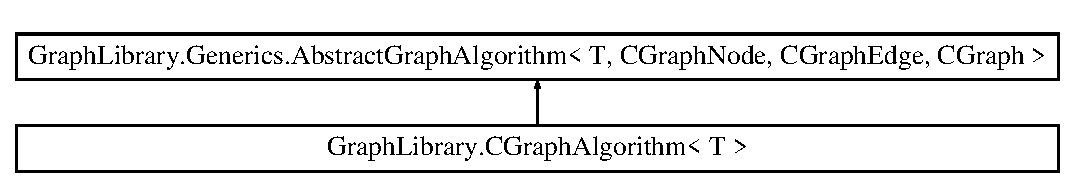
\includegraphics[height=2.000000cm]{class_graph_library_1_1_c_graph_algorithm}
\end{center}
\end{figure}
\subsection*{Public Member Functions}
\begin{DoxyCompactItemize}
\item 
\hypertarget{class_graph_library_1_1_c_graph_algorithm_aceea05e816d168d3a572fb03c71317c1}{}override object {\bfseries Visit\+Children} (\hyperlink{class_graph_library_1_1_c_graph_node}{C\+Graph\+Node} node)\label{class_graph_library_1_1_c_graph_algorithm_aceea05e816d168d3a572fb03c71317c1}

\end{DoxyCompactItemize}
\subsection*{Protected Member Functions}
\begin{DoxyCompactItemize}
\item 
\hypertarget{class_graph_library_1_1_c_graph_algorithm_ae4e0cf018a52938dca6f2e2fe1e4e6e1}{}{\bfseries C\+Graph\+Algorithm} (\hyperlink{class_graph_library_1_1_c_graph}{C\+Graph} graph)\label{class_graph_library_1_1_c_graph_algorithm_ae4e0cf018a52938dca6f2e2fe1e4e6e1}

\item 
\hyperlink{class_graph_library_1_1_c_graph_edge}{C\+Graph\+Edge} \hyperlink{class_graph_library_1_1_c_graph_algorithm_a0fc2d16057b2bbca80245546f0d2b5ad}{Edge} (\hyperlink{class_graph_library_1_1_c_graph_node}{C\+Graph\+Node} source, \hyperlink{class_graph_library_1_1_c_graph_node}{C\+Graph\+Node} target)
\begin{DoxyCompactList}\small\item\em Returns the specified edge from the graph to which the algorithm acts \end{DoxyCompactList}\end{DoxyCompactItemize}
\subsection*{Additional Inherited Members}


\subsection{Detailed Description}
This is an abstract class that represents algorithms that run on graphs with the following types of elements 1) \hyperlink{class_graph_library_1_1_c_graph_node}{C\+Graph\+Node} for nodes 2) \hyperlink{class_graph_library_1_1_c_graph_edge}{C\+Graph\+Edge} for edges 3) \hyperlink{class_graph_library_1_1_c_graph}{C\+Graph} for graphs 


\begin{DoxyTemplParams}{Template Parameters}
{\em T} & The type of element returned by the visit function\\
\hline
\end{DoxyTemplParams}
\begin{DoxySeeAlso}{See also}
Graph\+Library.\+Generics.\+Abstract\+Graph\+Algorithm$<$\+T,\+Graph\+Library.\+C\+Graph\+Node,\+Graph\+Library.\+C\+Graph\+Edge, Graph\+Library.\+C\+Graph$>$


\end{DoxySeeAlso}


\subsection{Member Function Documentation}
\hypertarget{class_graph_library_1_1_c_graph_algorithm_a0fc2d16057b2bbca80245546f0d2b5ad}{}\index{Graph\+Library\+::\+C\+Graph\+Algorithm@{Graph\+Library\+::\+C\+Graph\+Algorithm}!Edge@{Edge}}
\index{Edge@{Edge}!Graph\+Library\+::\+C\+Graph\+Algorithm@{Graph\+Library\+::\+C\+Graph\+Algorithm}}
\subsubsection[{Edge(\+C\+Graph\+Node source, C\+Graph\+Node target)}]{\setlength{\rightskip}{0pt plus 5cm}{\bf C\+Graph\+Edge} {\bf Graph\+Library.\+C\+Graph\+Algorithm}$<$ T $>$.Edge (
\begin{DoxyParamCaption}
\item[{{\bf C\+Graph\+Node}}]{source, }
\item[{{\bf C\+Graph\+Node}}]{target}
\end{DoxyParamCaption}
)\hspace{0.3cm}{\ttfamily [protected]}}\label{class_graph_library_1_1_c_graph_algorithm_a0fc2d16057b2bbca80245546f0d2b5ad}


Returns the specified edge from the graph to which the algorithm acts 


\begin{DoxyParams}{Parameters}
{\em source} & The source node\\
\hline
{\em target} & The target node\\
\hline
\end{DoxyParams}
\begin{DoxyReturn}{Returns}

\end{DoxyReturn}


The documentation for this class was generated from the following file\+:\begin{DoxyCompactItemize}
\item 
Graph\+Library/Graph\+Algorithm.\+cs\end{DoxyCompactItemize}

\hypertarget{class_graph_library_1_1_c_graph_edge}{}\section{Graph\+Library.\+C\+Graph\+Edge Class Reference}
\label{class_graph_library_1_1_c_graph_edge}\index{Graph\+Library.\+C\+Graph\+Edge@{Graph\+Library.\+C\+Graph\+Edge}}


A graph edges interconnects to Nodes ports that in sequence belong to a node The \hyperlink{class_graph_library_1_1_c_graph_edge}{C\+Graph\+Edge} class stores a reference to the source and target ports. And can provide through properties the source and target ports and nodes. It also provides given the port or node at the one side of the edge the corresponding port or node at the side.  


Inheritance diagram for Graph\+Library.\+C\+Graph\+Edge\+:\begin{figure}[H]
\begin{center}
\leavevmode
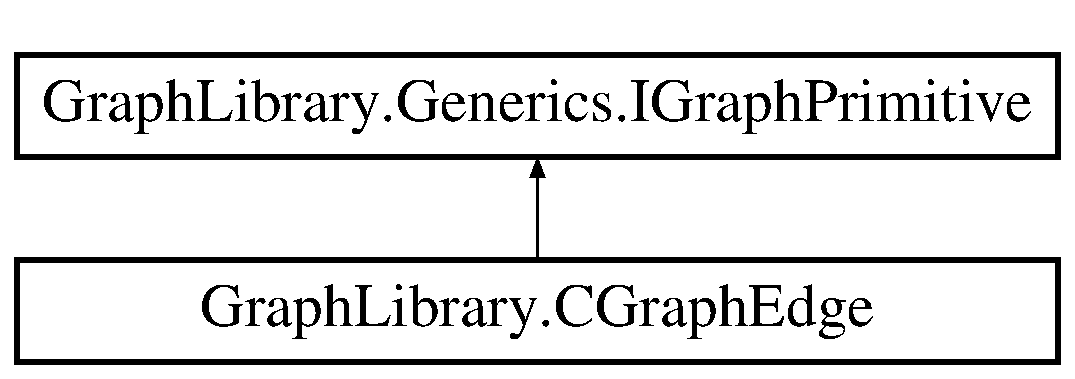
\includegraphics[height=2.000000cm]{class_graph_library_1_1_c_graph_edge}
\end{center}
\end{figure}
\subsection*{Public Member Functions}
\begin{DoxyCompactItemize}
\item 
\hyperlink{class_graph_library_1_1_c_graph_edge_a38f5e03ba556824dc271a9873b981d50}{C\+Graph\+Edge} (\hyperlink{class_graph_library_1_1_c_graph_node}{C\+Graph\+Node} source\+Node, \hyperlink{class_graph_library_1_1_c_graph_node}{C\+Graph\+Node} sink\+Node, \hyperlink{class_graph_library_1_1_c_graph}{C\+Graph} owner\+Graph, \hyperlink{namespace_graph_library_1_1_generics_a1bac729ea88e6f3925406df33f15d056}{Graph\+Type} edge\+Type=Graph\+Type.\+G\+T\+\_\+\+D\+I\+R\+E\+C\+T\+E\+D)
\begin{DoxyCompactList}\small\item\em Initializes a new instance of the \hyperlink{class_graph_library_1_1_c_graph_edge}{C\+Graph\+Edge} class. It creates an edge that connects the two nodes gives as parameters. \end{DoxyCompactList}\end{DoxyCompactItemize}
\subsection*{Properties}
\begin{DoxyCompactItemize}
\item 
object \hyperlink{class_graph_library_1_1_c_graph_edge_ad5cb4b4ef0423da4a0c2b156cf3fb3f7}{this\mbox{[}object index\mbox{]}}\hspace{0.3cm}{\ttfamily  \mbox{[}get, set\mbox{]}}
\begin{DoxyCompactList}\small\item\em Indexer returns the information referring to a specific algorithm object \end{DoxyCompactList}\item 
\hyperlink{class_graph_library_1_1_c_graph_node}{C\+Graph\+Node} \hyperlink{class_graph_library_1_1_c_graph_edge_a79ff7b9982b737ed66755c8baf51a31a}{M\+\_\+\+Source}\hspace{0.3cm}{\ttfamily  \mbox{[}get\mbox{]}}
\begin{DoxyCompactList}\small\item\em Represents the source node for directed graphs or one of the edge\textquotesingle{}s nodes of the undirected graph \end{DoxyCompactList}\item 
\hyperlink{class_graph_library_1_1_c_graph_node}{C\+Graph\+Node} \hyperlink{class_graph_library_1_1_c_graph_edge_a42c115e4937a251f524edc71a2b1ea7a}{M\+\_\+\+Target}\hspace{0.3cm}{\ttfamily  \mbox{[}get\mbox{]}}
\begin{DoxyCompactList}\small\item\em Represents the target node for directed graphs or one of the edge\textquotesingle{}s nodes of the undirected graph \end{DoxyCompactList}\item 
\hyperlink{class_graph_library_1_1_c_graph}{C\+Graph} \hyperlink{class_graph_library_1_1_c_graph_edge_aa1b8faca82c1d9fe1cafef980a1cbb82}{M\+\_\+\+Source\+Graph}\hspace{0.3cm}{\ttfamily  \mbox{[}get\mbox{]}}
\begin{DoxyCompactList}\small\item\em Represents the graph from where the edge originates \end{DoxyCompactList}\item 
\hyperlink{class_graph_library_1_1_c_graph}{C\+Graph} \hyperlink{class_graph_library_1_1_c_graph_edge_a0548b68a08517457f2bd5fbec3eb0628}{M\+\_\+\+Sink\+Graph}\hspace{0.3cm}{\ttfamily  \mbox{[}get\mbox{]}}
\begin{DoxyCompactList}\small\item\em Represents the graph to where the edge sinks \end{DoxyCompactList}\item 
\hyperlink{namespace_graph_library_1_1_generics_a1bac729ea88e6f3925406df33f15d056}{Graph\+Type} \hyperlink{class_graph_library_1_1_c_graph_edge_aeee79cda191cc06d78688848f6168e8c}{M\+\_\+\+Edge\+Type}\hspace{0.3cm}{\ttfamily  \mbox{[}get\mbox{]}}
\begin{DoxyCompactList}\small\item\em Represents the edge type. Can be directed or undirected \end{DoxyCompactList}\item 
virtual int \hyperlink{class_graph_library_1_1_c_graph_edge_a4a000bcf04e549dc33e522ace7facc63}{M\+\_\+\+Serial\+Number}\hspace{0.3cm}{\ttfamily  \mbox{[}get\mbox{]}}
\begin{DoxyCompactList}\small\item\em Returns the edge\textquotesingle{}s serial number \end{DoxyCompactList}\item 
\hyperlink{class_graph_library_1_1_c_graph}{C\+Graph} \hyperlink{class_graph_library_1_1_c_graph_edge_a59088a897b7cee66d1425b65e6bb945b}{M\+\_\+\+Owner\+Graph}\hspace{0.3cm}{\ttfamily  \mbox{[}get\mbox{]}}
\begin{DoxyCompactList}\small\item\em Represents the graph that owns the node \end{DoxyCompactList}\item 
\hyperlink{namespace_graph_library_1_1_generics_a919a165f16deccdd1b3d7e8a93423fbc}{Graph\+Element\+Type} \hyperlink{class_graph_library_1_1_c_graph_edge_a43275553517bb0104bfdfc7ea14984ea}{M\+\_\+\+Element\+Type}\hspace{0.3cm}{\ttfamily  \mbox{[}get\mbox{]}}
\begin{DoxyCompactList}\small\item\em Gets the type of the m\+\_\+ element. \end{DoxyCompactList}\end{DoxyCompactItemize}


\subsection{Detailed Description}
A graph edges interconnects to Nodes ports that in sequence belong to a node The \hyperlink{class_graph_library_1_1_c_graph_edge}{C\+Graph\+Edge} class stores a reference to the source and target ports. And can provide through properties the source and target ports and nodes. It also provides given the port or node at the one side of the edge the corresponding port or node at the side. 



\subsection{Constructor \& Destructor Documentation}
\hypertarget{class_graph_library_1_1_c_graph_edge_a38f5e03ba556824dc271a9873b981d50}{}\index{Graph\+Library\+::\+C\+Graph\+Edge@{Graph\+Library\+::\+C\+Graph\+Edge}!C\+Graph\+Edge@{C\+Graph\+Edge}}
\index{C\+Graph\+Edge@{C\+Graph\+Edge}!Graph\+Library\+::\+C\+Graph\+Edge@{Graph\+Library\+::\+C\+Graph\+Edge}}
\subsubsection[{C\+Graph\+Edge(\+C\+Graph\+Node source\+Node, C\+Graph\+Node sink\+Node, C\+Graph owner\+Graph, Graph\+Type edge\+Type=\+Graph\+Type.\+G\+T\+\_\+\+D\+I\+R\+E\+C\+T\+E\+D)}]{\setlength{\rightskip}{0pt plus 5cm}Graph\+Library.\+C\+Graph\+Edge.\+C\+Graph\+Edge (
\begin{DoxyParamCaption}
\item[{{\bf C\+Graph\+Node}}]{source\+Node, }
\item[{{\bf C\+Graph\+Node}}]{sink\+Node, }
\item[{{\bf C\+Graph}}]{owner\+Graph, }
\item[{{\bf Graph\+Type}}]{edge\+Type = {\ttfamily GraphType.GT\+\_\+DIRECTED}}
\end{DoxyParamCaption}
)}\label{class_graph_library_1_1_c_graph_edge_a38f5e03ba556824dc271a9873b981d50}


Initializes a new instance of the \hyperlink{class_graph_library_1_1_c_graph_edge}{C\+Graph\+Edge} class. It creates an edge that connects the two nodes gives as parameters. 


\begin{DoxyParams}{Parameters}
{\em source\+Node} & The source node.\\
\hline
{\em sink\+Node} & The sink node.\\
\hline
{\em owner\+Graph} & The owner graph.\\
\hline
{\em edge\+Type} & Type of the edge can be directed or undirected (optional default is D\+I\+R\+E\+C\+T\+E\+D).\\
\hline
\end{DoxyParams}

\begin{DoxyExceptions}{Exceptions}
{\em Null\+Reference\+Exception} & At least one of the nodes is null\\
\hline
\end{DoxyExceptions}


\subsection{Property Documentation}
\hypertarget{class_graph_library_1_1_c_graph_edge_aeee79cda191cc06d78688848f6168e8c}{}\index{Graph\+Library\+::\+C\+Graph\+Edge@{Graph\+Library\+::\+C\+Graph\+Edge}!M\+\_\+\+Edge\+Type@{M\+\_\+\+Edge\+Type}}
\index{M\+\_\+\+Edge\+Type@{M\+\_\+\+Edge\+Type}!Graph\+Library\+::\+C\+Graph\+Edge@{Graph\+Library\+::\+C\+Graph\+Edge}}
\subsubsection[{M\+\_\+\+Edge\+Type}]{\setlength{\rightskip}{0pt plus 5cm}{\bf Graph\+Type} Graph\+Library.\+C\+Graph\+Edge.\+M\+\_\+\+Edge\+Type\hspace{0.3cm}{\ttfamily [get]}}\label{class_graph_library_1_1_c_graph_edge_aeee79cda191cc06d78688848f6168e8c}


Represents the edge type. Can be directed or undirected 

The type of the m\+\_\+ edge. \hypertarget{class_graph_library_1_1_c_graph_edge_a43275553517bb0104bfdfc7ea14984ea}{}\index{Graph\+Library\+::\+C\+Graph\+Edge@{Graph\+Library\+::\+C\+Graph\+Edge}!M\+\_\+\+Element\+Type@{M\+\_\+\+Element\+Type}}
\index{M\+\_\+\+Element\+Type@{M\+\_\+\+Element\+Type}!Graph\+Library\+::\+C\+Graph\+Edge@{Graph\+Library\+::\+C\+Graph\+Edge}}
\subsubsection[{M\+\_\+\+Element\+Type}]{\setlength{\rightskip}{0pt plus 5cm}{\bf Graph\+Element\+Type} Graph\+Library.\+C\+Graph\+Edge.\+M\+\_\+\+Element\+Type\hspace{0.3cm}{\ttfamily [get]}}\label{class_graph_library_1_1_c_graph_edge_a43275553517bb0104bfdfc7ea14984ea}


Gets the type of the m\+\_\+ element. 

The type of the m\+\_\+ element. \hypertarget{class_graph_library_1_1_c_graph_edge_a59088a897b7cee66d1425b65e6bb945b}{}\index{Graph\+Library\+::\+C\+Graph\+Edge@{Graph\+Library\+::\+C\+Graph\+Edge}!M\+\_\+\+Owner\+Graph@{M\+\_\+\+Owner\+Graph}}
\index{M\+\_\+\+Owner\+Graph@{M\+\_\+\+Owner\+Graph}!Graph\+Library\+::\+C\+Graph\+Edge@{Graph\+Library\+::\+C\+Graph\+Edge}}
\subsubsection[{M\+\_\+\+Owner\+Graph}]{\setlength{\rightskip}{0pt plus 5cm}{\bf C\+Graph} Graph\+Library.\+C\+Graph\+Edge.\+M\+\_\+\+Owner\+Graph\hspace{0.3cm}{\ttfamily [get]}}\label{class_graph_library_1_1_c_graph_edge_a59088a897b7cee66d1425b65e6bb945b}


Represents the graph that owns the node 

The owner graph. \hypertarget{class_graph_library_1_1_c_graph_edge_a4a000bcf04e549dc33e522ace7facc63}{}\index{Graph\+Library\+::\+C\+Graph\+Edge@{Graph\+Library\+::\+C\+Graph\+Edge}!M\+\_\+\+Serial\+Number@{M\+\_\+\+Serial\+Number}}
\index{M\+\_\+\+Serial\+Number@{M\+\_\+\+Serial\+Number}!Graph\+Library\+::\+C\+Graph\+Edge@{Graph\+Library\+::\+C\+Graph\+Edge}}
\subsubsection[{M\+\_\+\+Serial\+Number}]{\setlength{\rightskip}{0pt plus 5cm}virtual int Graph\+Library.\+C\+Graph\+Edge.\+M\+\_\+\+Serial\+Number\hspace{0.3cm}{\ttfamily [get]}}\label{class_graph_library_1_1_c_graph_edge_a4a000bcf04e549dc33e522ace7facc63}


Returns the edge\textquotesingle{}s serial number 

\begin{DoxyReturn}{Returns}

\end{DoxyReturn}
\hypertarget{class_graph_library_1_1_c_graph_edge_a0548b68a08517457f2bd5fbec3eb0628}{}\index{Graph\+Library\+::\+C\+Graph\+Edge@{Graph\+Library\+::\+C\+Graph\+Edge}!M\+\_\+\+Sink\+Graph@{M\+\_\+\+Sink\+Graph}}
\index{M\+\_\+\+Sink\+Graph@{M\+\_\+\+Sink\+Graph}!Graph\+Library\+::\+C\+Graph\+Edge@{Graph\+Library\+::\+C\+Graph\+Edge}}
\subsubsection[{M\+\_\+\+Sink\+Graph}]{\setlength{\rightskip}{0pt plus 5cm}{\bf C\+Graph} Graph\+Library.\+C\+Graph\+Edge.\+M\+\_\+\+Sink\+Graph\hspace{0.3cm}{\ttfamily [get]}}\label{class_graph_library_1_1_c_graph_edge_a0548b68a08517457f2bd5fbec3eb0628}


Represents the graph to where the edge sinks 

The m\+\_\+ sink graph. \hypertarget{class_graph_library_1_1_c_graph_edge_a79ff7b9982b737ed66755c8baf51a31a}{}\index{Graph\+Library\+::\+C\+Graph\+Edge@{Graph\+Library\+::\+C\+Graph\+Edge}!M\+\_\+\+Source@{M\+\_\+\+Source}}
\index{M\+\_\+\+Source@{M\+\_\+\+Source}!Graph\+Library\+::\+C\+Graph\+Edge@{Graph\+Library\+::\+C\+Graph\+Edge}}
\subsubsection[{M\+\_\+\+Source}]{\setlength{\rightskip}{0pt plus 5cm}{\bf C\+Graph\+Node} Graph\+Library.\+C\+Graph\+Edge.\+M\+\_\+\+Source\hspace{0.3cm}{\ttfamily [get]}}\label{class_graph_library_1_1_c_graph_edge_a79ff7b9982b737ed66755c8baf51a31a}


Represents the source node for directed graphs or one of the edge\textquotesingle{}s nodes of the undirected graph 

Returns a reference to the source node \hypertarget{class_graph_library_1_1_c_graph_edge_aa1b8faca82c1d9fe1cafef980a1cbb82}{}\index{Graph\+Library\+::\+C\+Graph\+Edge@{Graph\+Library\+::\+C\+Graph\+Edge}!M\+\_\+\+Source\+Graph@{M\+\_\+\+Source\+Graph}}
\index{M\+\_\+\+Source\+Graph@{M\+\_\+\+Source\+Graph}!Graph\+Library\+::\+C\+Graph\+Edge@{Graph\+Library\+::\+C\+Graph\+Edge}}
\subsubsection[{M\+\_\+\+Source\+Graph}]{\setlength{\rightskip}{0pt plus 5cm}{\bf C\+Graph} Graph\+Library.\+C\+Graph\+Edge.\+M\+\_\+\+Source\+Graph\hspace{0.3cm}{\ttfamily [get]}}\label{class_graph_library_1_1_c_graph_edge_aa1b8faca82c1d9fe1cafef980a1cbb82}


Represents the graph from where the edge originates 

The m\+\_\+ source graph. \hypertarget{class_graph_library_1_1_c_graph_edge_a42c115e4937a251f524edc71a2b1ea7a}{}\index{Graph\+Library\+::\+C\+Graph\+Edge@{Graph\+Library\+::\+C\+Graph\+Edge}!M\+\_\+\+Target@{M\+\_\+\+Target}}
\index{M\+\_\+\+Target@{M\+\_\+\+Target}!Graph\+Library\+::\+C\+Graph\+Edge@{Graph\+Library\+::\+C\+Graph\+Edge}}
\subsubsection[{M\+\_\+\+Target}]{\setlength{\rightskip}{0pt plus 5cm}{\bf C\+Graph\+Node} Graph\+Library.\+C\+Graph\+Edge.\+M\+\_\+\+Target\hspace{0.3cm}{\ttfamily [get]}}\label{class_graph_library_1_1_c_graph_edge_a42c115e4937a251f524edc71a2b1ea7a}


Represents the target node for directed graphs or one of the edge\textquotesingle{}s nodes of the undirected graph 

Returns a reference to the target node \hypertarget{class_graph_library_1_1_c_graph_edge_ad5cb4b4ef0423da4a0c2b156cf3fb3f7}{}\index{Graph\+Library\+::\+C\+Graph\+Edge@{Graph\+Library\+::\+C\+Graph\+Edge}!this\mbox{[}object index\mbox{]}@{this[object index]}}
\index{this\mbox{[}object index\mbox{]}@{this[object index]}!Graph\+Library\+::\+C\+Graph\+Edge@{Graph\+Library\+::\+C\+Graph\+Edge}}
\subsubsection[{this[object index]}]{\setlength{\rightskip}{0pt plus 5cm}object Graph\+Library.\+C\+Graph\+Edge.\+this\mbox{[}object index\mbox{]}\hspace{0.3cm}{\ttfamily [get]}, {\ttfamily [set]}}\label{class_graph_library_1_1_c_graph_edge_ad5cb4b4ef0423da4a0c2b156cf3fb3f7}


Indexer returns the information referring to a specific algorithm object 


\begin{DoxyParams}{Parameters}
{\em index} & Algorithm object\\
\hline
\end{DoxyParams}
\begin{DoxyReturn}{Returns}
Returns the information that the algorithm indicated by \char`\"{}index\char`\"{} stored in the edge
\end{DoxyReturn}


The documentation for this class was generated from the following file\+:\begin{DoxyCompactItemize}
\item 
Graph\+Library/Graph\+Elements.\+cs\end{DoxyCompactItemize}

\hypertarget{class_graph_library_1_1_c_graph_iterators_factory}{}\section{Graph\+Library.\+C\+Graph\+Iterators\+Factory Class Reference}
\label{class_graph_library_1_1_c_graph_iterators_factory}\index{Graph\+Library.\+C\+Graph\+Iterators\+Factory@{Graph\+Library.\+C\+Graph\+Iterators\+Factory}}
Inheritance diagram for Graph\+Library.\+C\+Graph\+Iterators\+Factory\+:\begin{figure}[H]
\begin{center}
\leavevmode
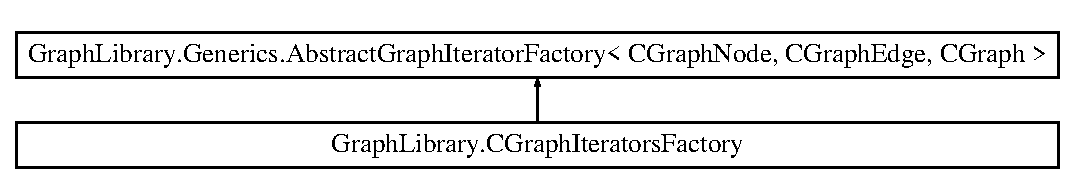
\includegraphics[height=2.000000cm]{class_graph_library_1_1_c_graph_iterators_factory}
\end{center}
\end{figure}
\subsection*{Public Member Functions}
\begin{DoxyCompactItemize}
\item 
\hypertarget{class_graph_library_1_1_c_graph_iterators_factory_adcbb1187f8ff64e6eac58d04b37ad928}{}{\bfseries C\+Graph\+Iterators\+Factory} (\hyperlink{class_graph_library_1_1_c_graph}{C\+Graph} graph)\label{class_graph_library_1_1_c_graph_iterators_factory_adcbb1187f8ff64e6eac58d04b37ad928}

\item 
\hypertarget{class_graph_library_1_1_c_graph_iterators_factory_aa73589aa48093ff9f40695e11c2fca43}{}override \hyperlink{class_graph_library_1_1_c_it___successors}{C\+It\+\_\+\+Successors} {\bfseries Create\+Successors\+Iterator} (\hyperlink{class_graph_library_1_1_c_graph_node}{C\+Graph\+Node} node)\label{class_graph_library_1_1_c_graph_iterators_factory_aa73589aa48093ff9f40695e11c2fca43}

\item 
\hypertarget{class_graph_library_1_1_c_graph_iterators_factory_a7c2263e641d6255778b4c7303317102d}{}override \hyperlink{class_graph_library_1_1_c_it___predecessors}{C\+It\+\_\+\+Predecessors} {\bfseries Create\+Predecessors\+Iterator} (\hyperlink{class_graph_library_1_1_c_graph_node}{C\+Graph\+Node} node)\label{class_graph_library_1_1_c_graph_iterators_factory_a7c2263e641d6255778b4c7303317102d}

\item 
\hypertarget{class_graph_library_1_1_c_graph_iterators_factory_a3eee9436be4f136da48e9fe708bb1116}{}override \hyperlink{class_graph_library_1_1_c_it___graph_edges}{C\+It\+\_\+\+Graph\+Edges} {\bfseries Create\+Graph\+Edges\+Iterator} ()\label{class_graph_library_1_1_c_graph_iterators_factory_a3eee9436be4f136da48e9fe708bb1116}

\item 
\hypertarget{class_graph_library_1_1_c_graph_iterators_factory_a4a5bdbb305ef3a13a9be4524a3fe3665}{}override \hyperlink{class_graph_library_1_1_c_it___graph_nodes}{C\+It\+\_\+\+Graph\+Nodes} {\bfseries Create\+Graph\+Nodes\+Iterator} ()\label{class_graph_library_1_1_c_graph_iterators_factory_a4a5bdbb305ef3a13a9be4524a3fe3665}

\item 
\hypertarget{class_graph_library_1_1_c_graph_iterators_factory_a789fbd1fef32e6bcb5418f32e42f01a5}{}override \hyperlink{class_graph_library_1_1_c_it___graph_root_nodes}{C\+It\+\_\+\+Graph\+Root\+Nodes} {\bfseries Create\+Graph\+Root\+Nodes\+Iterator} ()\label{class_graph_library_1_1_c_graph_iterators_factory_a789fbd1fef32e6bcb5418f32e42f01a5}

\item 
\hypertarget{class_graph_library_1_1_c_graph_iterators_factory_aefe770767765599b969b5202f340dd9a}{}override \hyperlink{class_graph_library_1_1_c_it___graph_leaf_nodes}{C\+It\+\_\+\+Graph\+Leaf\+Nodes} {\bfseries Create\+Graph\+Leaf\+Nodes\+Iterator} ()\label{class_graph_library_1_1_c_graph_iterators_factory_aefe770767765599b969b5202f340dd9a}

\item 
\hypertarget{class_graph_library_1_1_c_graph_iterators_factory_afe9896022dd8c954737aee30bec66fbe}{}override \hyperlink{class_graph_library_1_1_c_it___graph_d_f_s}{C\+It\+\_\+\+Graph\+D\+F\+S} {\bfseries Create\+Graph\+Dfs\+Iterator} ()\label{class_graph_library_1_1_c_graph_iterators_factory_afe9896022dd8c954737aee30bec66fbe}

\item 
\hypertarget{class_graph_library_1_1_c_graph_iterators_factory_a2c970fc96edbb626f1b6875413d473f4}{}override \hyperlink{class_graph_library_1_1_c_it___graph_b_f_s}{C\+It\+\_\+\+Graph\+B\+F\+S} {\bfseries Create\+Graph\+Bfs\+Iterator} (\hyperlink{class_graph_library_1_1_c_graph_node}{C\+Graph\+Node} start\+Node)\label{class_graph_library_1_1_c_graph_iterators_factory_a2c970fc96edbb626f1b6875413d473f4}

\end{DoxyCompactItemize}
\subsection*{Additional Inherited Members}


The documentation for this class was generated from the following file\+:\begin{DoxyCompactItemize}
\item 
Graph\+Library/Graph\+Iterators\+Factory.\+cs\end{DoxyCompactItemize}

\hypertarget{class_graph_library_1_1_c_graph_labeling}{}\section{Graph\+Library.\+C\+Graph\+Labeling$<$ T $>$ Class Template Reference}
\label{class_graph_library_1_1_c_graph_labeling}\index{Graph\+Library.\+C\+Graph\+Labeling$<$ T $>$@{Graph\+Library.\+C\+Graph\+Labeling$<$ T $>$}}


This class provides general graph labelling capabilities. It doesn\textquotesingle{}t follow a specific strategy to label nodes/edges. It just implements the default version of Set\+Label methods for the class \hyperlink{class_graph_library_1_1_c_graph}{C\+Graph}. (This class is specific to \hyperlink{class_graph_library_1_1_c_graph}{C\+Graph} class)  


Inheritance diagram for Graph\+Library.\+C\+Graph\+Labeling$<$ T $>$\+:\begin{figure}[H]
\begin{center}
\leavevmode
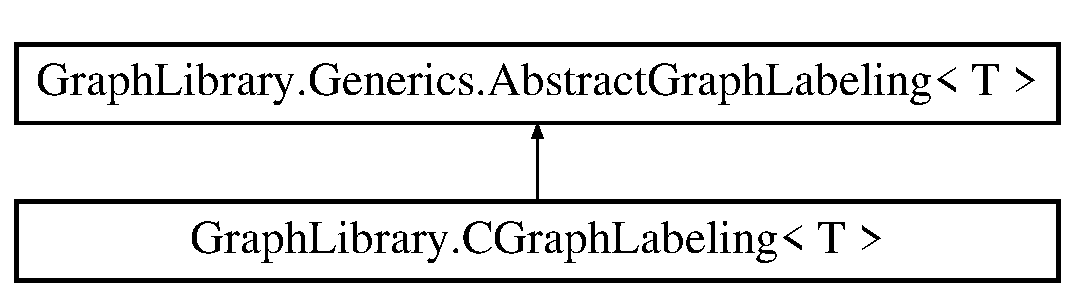
\includegraphics[height=2.000000cm]{class_graph_library_1_1_c_graph_labeling}
\end{center}
\end{figure}
\subsection*{Public Member Functions}
\begin{DoxyCompactItemize}
\item 
\hypertarget{class_graph_library_1_1_c_graph_labeling_a44b3f485518381900722bd80796a3f8c}{}{\bfseries C\+Graph\+Labeling} (\hyperlink{class_graph_library_1_1_c_graph}{C\+Graph} graph)\label{class_graph_library_1_1_c_graph_labeling_a44b3f485518381900722bd80796a3f8c}

\item 
override void \hyperlink{class_graph_library_1_1_c_graph_labeling_accff39c0e47f50e582586e91da5a217f}{Set\+Label} (T element, string label)
\begin{DoxyCompactList}\small\item\em Sets the label of the given element. The element must exist in the graph and the label must not be already used by another element of the same type \end{DoxyCompactList}\item 
override void \hyperlink{class_graph_library_1_1_c_graph_labeling_abc0c9a99fd0ed7d21d3294c017587888}{Set\+Label} (int serial\+Number, \hyperlink{namespace_graph_library_1_1_generics_a919a165f16deccdd1b3d7e8a93423fbc}{Graph\+Element\+Type} element\+Type, string label)
\begin{DoxyCompactList}\small\item\em Sets the label of the element with the given serialnumber. The element must exist in the graph and the label must not be already used by another element of the same type (node, edge) \end{DoxyCompactList}\end{DoxyCompactItemize}
\subsection*{Protected Member Functions}
\begin{DoxyCompactItemize}
\item 
override void \hyperlink{class_graph_library_1_1_c_graph_labeling_aacfaf94dbe1fe9e65e95929a03d9f960}{Label\+Elements} ()
\begin{DoxyCompactList}\small\item\em Gives the initial mapping of labels to elements. Called by the constructor. Must be defined in subclasses The version in this class doesn\textquotesingle{}t do anything \end{DoxyCompactList}\end{DoxyCompactItemize}
\subsection*{Protected Attributes}
\begin{DoxyCompactItemize}
\item 
\hypertarget{class_graph_library_1_1_c_graph_labeling_a086fef646e5affb6ebdc82459e809157}{}\hyperlink{class_graph_library_1_1_c_graph}{C\+Graph} {\bfseries m\+\_\+\+Graph}\label{class_graph_library_1_1_c_graph_labeling_a086fef646e5affb6ebdc82459e809157}

\end{DoxyCompactItemize}


\subsection{Detailed Description}
This class provides general graph labelling capabilities. It doesn\textquotesingle{}t follow a specific strategy to label nodes/edges. It just implements the default version of Set\+Label methods for the class \hyperlink{class_graph_library_1_1_c_graph}{C\+Graph}. (This class is specific to \hyperlink{class_graph_library_1_1_c_graph}{C\+Graph} class) 


\begin{DoxyTemplParams}{Template Parameters}
{\em T} & Type of element to label\\
\hline
\end{DoxyTemplParams}
\begin{DoxySeeAlso}{See also}
Graph\+Library.\+Generics.\+Abstract\+Graph\+Labeling$<$\+T$>$


\end{DoxySeeAlso}
\begin{Desc}
\item[Type Constraints]\begin{description}
\item[{\em T} : {\em I\+Graph\+Primitive}]\end{description}
\end{Desc}


\subsection{Member Function Documentation}
\hypertarget{class_graph_library_1_1_c_graph_labeling_aacfaf94dbe1fe9e65e95929a03d9f960}{}\index{Graph\+Library\+::\+C\+Graph\+Labeling@{Graph\+Library\+::\+C\+Graph\+Labeling}!Label\+Elements@{Label\+Elements}}
\index{Label\+Elements@{Label\+Elements}!Graph\+Library\+::\+C\+Graph\+Labeling@{Graph\+Library\+::\+C\+Graph\+Labeling}}
\subsubsection[{Label\+Elements()}]{\setlength{\rightskip}{0pt plus 5cm}override void {\bf Graph\+Library.\+C\+Graph\+Labeling}$<$ T $>$.Label\+Elements (
\begin{DoxyParamCaption}
{}
\end{DoxyParamCaption}
)\hspace{0.3cm}{\ttfamily [protected]}, {\ttfamily [virtual]}}\label{class_graph_library_1_1_c_graph_labeling_aacfaf94dbe1fe9e65e95929a03d9f960}


Gives the initial mapping of labels to elements. Called by the constructor. Must be defined in subclasses The version in this class doesn\textquotesingle{}t do anything 



Implements \hyperlink{class_graph_library_1_1_generics_1_1_abstract_graph_labeling_a890775a0a91077bedd4330df8ddafe48}{Graph\+Library.\+Generics.\+Abstract\+Graph\+Labeling$<$ T $>$}.

\hypertarget{class_graph_library_1_1_c_graph_labeling_accff39c0e47f50e582586e91da5a217f}{}\index{Graph\+Library\+::\+C\+Graph\+Labeling@{Graph\+Library\+::\+C\+Graph\+Labeling}!Set\+Label@{Set\+Label}}
\index{Set\+Label@{Set\+Label}!Graph\+Library\+::\+C\+Graph\+Labeling@{Graph\+Library\+::\+C\+Graph\+Labeling}}
\subsubsection[{Set\+Label(\+T element, string label)}]{\setlength{\rightskip}{0pt plus 5cm}override void {\bf Graph\+Library.\+C\+Graph\+Labeling}$<$ T $>$.Set\+Label (
\begin{DoxyParamCaption}
\item[{T}]{element, }
\item[{string}]{label}
\end{DoxyParamCaption}
)}\label{class_graph_library_1_1_c_graph_labeling_accff39c0e47f50e582586e91da5a217f}


Sets the label of the given element. The element must exist in the graph and the label must not be already used by another element of the same type 


\begin{DoxyParams}{Parameters}
{\em element} & The element.\\
\hline
{\em label} & The label.\\
\hline
\end{DoxyParams}

\begin{DoxyExceptions}{Exceptions}
{\em System.\+Collections.\+Generic.\+Key\+Not\+Found\+Exception} & Element does not exist or label already exists in the graph\\
\hline
\end{DoxyExceptions}
\hypertarget{class_graph_library_1_1_c_graph_labeling_abc0c9a99fd0ed7d21d3294c017587888}{}\index{Graph\+Library\+::\+C\+Graph\+Labeling@{Graph\+Library\+::\+C\+Graph\+Labeling}!Set\+Label@{Set\+Label}}
\index{Set\+Label@{Set\+Label}!Graph\+Library\+::\+C\+Graph\+Labeling@{Graph\+Library\+::\+C\+Graph\+Labeling}}
\subsubsection[{Set\+Label(int serial\+Number, Graph\+Element\+Type element\+Type, string label)}]{\setlength{\rightskip}{0pt plus 5cm}override void {\bf Graph\+Library.\+C\+Graph\+Labeling}$<$ T $>$.Set\+Label (
\begin{DoxyParamCaption}
\item[{int}]{serial\+Number, }
\item[{{\bf Graph\+Element\+Type}}]{element\+Type, }
\item[{string}]{label}
\end{DoxyParamCaption}
)\hspace{0.3cm}{\ttfamily [virtual]}}\label{class_graph_library_1_1_c_graph_labeling_abc0c9a99fd0ed7d21d3294c017587888}


Sets the label of the element with the given serialnumber. The element must exist in the graph and the label must not be already used by another element of the same type (node, edge) 


\begin{DoxyParams}{Parameters}
{\em serial\+Number} & The serial number.\\
\hline
{\em label} & The label.\\
\hline
\end{DoxyParams}


Implements \hyperlink{class_graph_library_1_1_generics_1_1_abstract_graph_labeling_a268a30e52ddd582947c6e35766627e73}{Graph\+Library.\+Generics.\+Abstract\+Graph\+Labeling$<$ T $>$}.



The documentation for this class was generated from the following file\+:\begin{DoxyCompactItemize}
\item 
Graph\+Library/Graph\+Labeling.\+cs\end{DoxyCompactItemize}

\hypertarget{class_graph_library_1_1_c_graph_node}{}\section{Graph\+Library.\+C\+Graph\+Node Class Reference}
\label{class_graph_library_1_1_c_graph_node}\index{Graph\+Library.\+C\+Graph\+Node@{Graph\+Library.\+C\+Graph\+Node}}


Represents a graph node .  


Inheritance diagram for Graph\+Library.\+C\+Graph\+Node\+:\begin{figure}[H]
\begin{center}
\leavevmode
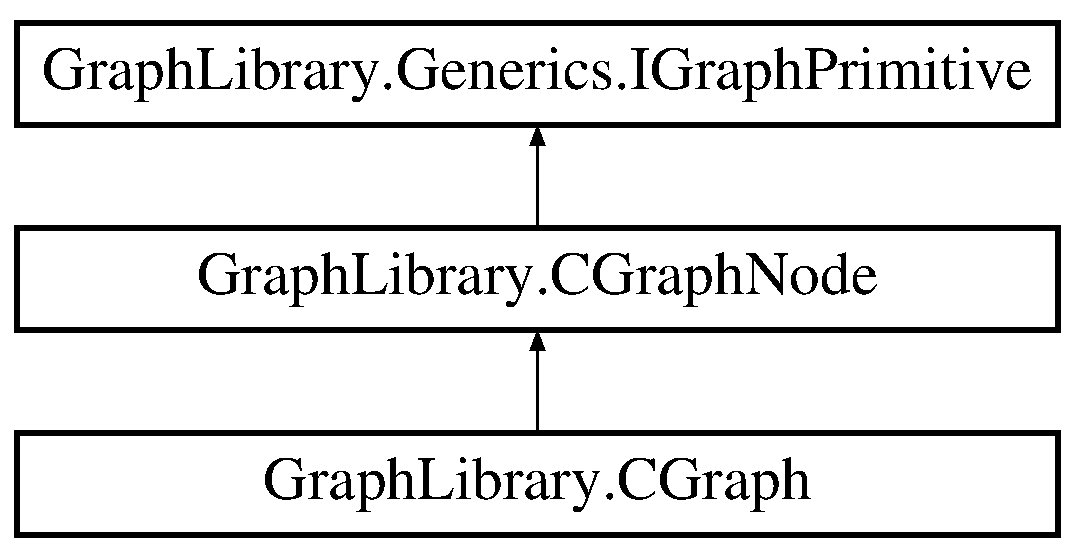
\includegraphics[height=3.000000cm]{class_graph_library_1_1_c_graph_node}
\end{center}
\end{figure}
\subsection*{Public Member Functions}
\begin{DoxyCompactItemize}
\item 
\hyperlink{class_graph_library_1_1_c_graph_node_aa1d9c216b6466f4bd34b6a6d761a5a83}{C\+Graph\+Node} (\hyperlink{class_graph_library_1_1_c_graph}{C\+Graph} owner\+Graph)
\begin{DoxyCompactList}\small\item\em Initializes a new instance of the \hyperlink{class_graph_library_1_1_c_graph_node}{C\+Graph\+Node} class. \end{DoxyCompactList}\item 
void \hyperlink{class_graph_library_1_1_c_graph_node_ad710e8d3562812517fd4558518442990}{Add\+Successor} (\hyperlink{class_graph_library_1_1_c_graph_node}{C\+Graph\+Node} target, \hyperlink{namespace_graph_library_1_1_generics_a1bac729ea88e6f3925406df33f15d056}{Graph\+Type} edgetype, \hyperlink{class_graph_library_1_1_c_graph}{C\+Graph} foreign\+Graph=null)
\begin{DoxyCompactList}\small\item\em Adds the successor to the current node. \end{DoxyCompactList}\item 
\hyperlink{class_graph_library_1_1_c_graph_node}{C\+Graph\+Node} \hyperlink{class_graph_library_1_1_c_graph_node_a8264470518ce61df1bc111cdafafba68}{Successor} (int index)
\begin{DoxyCompactList}\small\item\em Returns the i-\/th native successor in the list \end{DoxyCompactList}\item 
void \hyperlink{class_graph_library_1_1_c_graph_node_a5d03becd7eb30cecb2074d4d7c9e818c}{Add\+Predecessor} (\hyperlink{class_graph_library_1_1_c_graph_node}{C\+Graph\+Node} source, \hyperlink{namespace_graph_library_1_1_generics_a1bac729ea88e6f3925406df33f15d056}{Graph\+Type} edgetype, \hyperlink{class_graph_library_1_1_c_graph}{C\+Graph} foreign\+Graph=null)
\begin{DoxyCompactList}\small\item\em Adds the predecessor to the current node. \end{DoxyCompactList}\item 
\hyperlink{class_graph_library_1_1_c_graph_node}{C\+Graph\+Node} \hyperlink{class_graph_library_1_1_c_graph_node_ab37e7c5b8dc940a2cfd8e301f50d633e}{Predeccessor} (int index)
\begin{DoxyCompactList}\small\item\em Returns the i-\/th predecessor in the list of predecessors \end{DoxyCompactList}\item 
void \hyperlink{class_graph_library_1_1_c_graph_node_ad2b029d744be615c8de5c8f396154de1}{Set\+Label\+Context} (object context)
\begin{DoxyCompactList}\small\item\em Sets the label context. \end{DoxyCompactList}\item 
string \hyperlink{class_graph_library_1_1_c_graph_node_af75b2590fa8bdce8c81c56f645f121a0}{To\+String} (object labeler)
\begin{DoxyCompactList}\small\item\em Returns a System.\+String that represents the label of the node given by the specifier labeler object C\+Graph\+Labeling$<$\+T$>$ \end{DoxyCompactList}\item 
override string \hyperlink{class_graph_library_1_1_c_graph_node_a3e26e00defb555fc26c9e9f7eaf003f5}{To\+String} ()
\begin{DoxyCompactList}\small\item\em Returns the label of the node. If a labeler object is specified in the member variable m\+\_\+label\+Context then the labeler object provides the label otherwise an ad-\/hoc label is provided. \end{DoxyCompactList}\item 
override int \hyperlink{class_graph_library_1_1_c_graph_node_a77205fe388f8b37cb45ceadefe40bcb0}{Get\+Hash\+Code} ()
\begin{DoxyCompactList}\small\item\em Returns a hash code for this instance. It actually returns the serial number of the node which is unique for each graph element \end{DoxyCompactList}\end{DoxyCompactItemize}
\subsection*{Protected Attributes}
\begin{DoxyCompactItemize}
\item 
bool \hyperlink{class_graph_library_1_1_c_graph_node_aec1f789c7ef7cf0e34d456eb3e7a9ccb}{m\+\_\+is\+Compound\+Node} = false
\begin{DoxyCompactList}\small\item\em It is true if the node is a graph. \end{DoxyCompactList}\end{DoxyCompactItemize}
\subsection*{Static Protected Attributes}
\begin{DoxyCompactItemize}
\item 
static object \hyperlink{class_graph_library_1_1_c_graph_node_a6778251b91c25126259a1c838324eea4}{m\+\_\+label\+Context} =null
\begin{DoxyCompactList}\small\item\em The label context is the the object that provides labels to the graph nodes. It could be and algorithm, printer, etc \end{DoxyCompactList}\end{DoxyCompactItemize}
\subsection*{Properties}
\begin{DoxyCompactItemize}
\item 
int \hyperlink{class_graph_library_1_1_c_graph_node_a1a877b0e26c037d267bcdb4eb17087ae}{M\+\_\+\+Number\+Of\+Successors}\hspace{0.3cm}{\ttfamily  \mbox{[}get\mbox{]}}
\begin{DoxyCompactList}\small\item\em Returns the number of native (nodes that belong to the same graph as the current node) successors \end{DoxyCompactList}\item 
List$<$ \hyperlink{class_graph_library_1_1_c_graph_node}{C\+Graph\+Node} $>$ \hyperlink{class_graph_library_1_1_c_graph_node_a5f3bca4eb56bce992ef018820bdd20c4}{M\+\_\+\+Successors}\hspace{0.3cm}{\ttfamily  \mbox{[}get\mbox{]}}
\begin{DoxyCompactList}\small\item\em Returns the Node\textquotesingle{}s native successors in a list. The list is allocated inside the getter\textquotesingle{}s code \end{DoxyCompactList}\item 
int \hyperlink{class_graph_library_1_1_c_graph_node_ac0f1e583a6b672b03e146cb730b1682a}{M\+\_\+\+Number\+Of\+Predecessors}\hspace{0.3cm}{\ttfamily  \mbox{[}get\mbox{]}}
\begin{DoxyCompactList}\small\item\em Returns the number of native (nodes that belong to the same graph as the current node) predecessors \end{DoxyCompactList}\item 
List$<$ \hyperlink{class_graph_library_1_1_c_graph_node}{C\+Graph\+Node} $>$ \hyperlink{class_graph_library_1_1_c_graph_node_a428ee478ef04cd06956671a94dafdbc5}{M\+\_\+\+Predecessors}\hspace{0.3cm}{\ttfamily  \mbox{[}get\mbox{]}}
\begin{DoxyCompactList}\small\item\em Returns the Node\textquotesingle{}s native predecessors in a list \end{DoxyCompactList}\item 
List$<$ \hyperlink{class_graph_library_1_1_c_graph_edge}{C\+Graph\+Edge} $>$ \hyperlink{class_graph_library_1_1_c_graph_node_af1dd68175bb884b10c5972c57b3c243f}{M\+\_\+\+Foreign\+Edges}\hspace{0.3cm}{\ttfamily  \mbox{[}get\mbox{]}}
\begin{DoxyCompactList}\small\item\em Gets the foreign edges to which this node connects. Returns a list with the foreign edges \end{DoxyCompactList}\item 
\hyperlink{class_graph_library_1_1_c_graph}{C\+Graph} \hyperlink{class_graph_library_1_1_c_graph_node_af74860380cdc7a69e9ec6634e2ccdc48}{M\+\_\+\+Owner\+Graph}\hspace{0.3cm}{\ttfamily  \mbox{[}get, set\mbox{]}}
\begin{DoxyCompactList}\small\item\em Represents the owner graph of the node \end{DoxyCompactList}\item 
virtual int \hyperlink{class_graph_library_1_1_c_graph_node_a43e9c4162fb28defd6c0193f2222d199}{M\+\_\+\+Serial\+Number}\hspace{0.3cm}{\ttfamily  \mbox{[}get\mbox{]}}
\begin{DoxyCompactList}\small\item\em Returns the node\textquotesingle{}s serial number. \end{DoxyCompactList}\item 
bool \hyperlink{class_graph_library_1_1_c_graph_node_a8b1a7e4ee0887d7555ed8e7fc183cf21}{M\+\_\+\+Is\+Compound\+Node}\hspace{0.3cm}{\ttfamily  \mbox{[}get\mbox{]}}
\begin{DoxyCompactList}\small\item\em Is a boolean attribute that indicates weather the node is compound \end{DoxyCompactList}\item 
\hyperlink{namespace_graph_library_1_1_generics_a919a165f16deccdd1b3d7e8a93423fbc}{Graph\+Element\+Type} \hyperlink{class_graph_library_1_1_c_graph_node_a1b13fbb13f63117f18610da1fe6b86ac}{M\+\_\+\+Element\+Type}\hspace{0.3cm}{\ttfamily  \mbox{[}get\mbox{]}}
\begin{DoxyCompactList}\small\item\em Gets the type of the m\+\_\+ element. \end{DoxyCompactList}\item 
object \hyperlink{class_graph_library_1_1_c_graph_node_a2e5ed7afca428365f7aef68611f852fe}{this\mbox{[}object index\mbox{]}}\hspace{0.3cm}{\ttfamily  \mbox{[}get, set\mbox{]}}
\begin{DoxyCompactList}\small\item\em Indexer returns the information referring to a specific algorithm object \end{DoxyCompactList}\end{DoxyCompactItemize}


\subsection{Detailed Description}
Represents a graph node . 



\subsection{Constructor \& Destructor Documentation}
\hypertarget{class_graph_library_1_1_c_graph_node_aa1d9c216b6466f4bd34b6a6d761a5a83}{}\index{Graph\+Library\+::\+C\+Graph\+Node@{Graph\+Library\+::\+C\+Graph\+Node}!C\+Graph\+Node@{C\+Graph\+Node}}
\index{C\+Graph\+Node@{C\+Graph\+Node}!Graph\+Library\+::\+C\+Graph\+Node@{Graph\+Library\+::\+C\+Graph\+Node}}
\subsubsection[{C\+Graph\+Node(\+C\+Graph owner\+Graph)}]{\setlength{\rightskip}{0pt plus 5cm}Graph\+Library.\+C\+Graph\+Node.\+C\+Graph\+Node (
\begin{DoxyParamCaption}
\item[{{\bf C\+Graph}}]{owner\+Graph}
\end{DoxyParamCaption}
)}\label{class_graph_library_1_1_c_graph_node_aa1d9c216b6466f4bd34b6a6d761a5a83}


Initializes a new instance of the \hyperlink{class_graph_library_1_1_c_graph_node}{C\+Graph\+Node} class. 


\begin{DoxyParams}{Parameters}
{\em owner\+Graph} & The owner graph.\\
\hline
\end{DoxyParams}


\subsection{Member Function Documentation}
\hypertarget{class_graph_library_1_1_c_graph_node_a5d03becd7eb30cecb2074d4d7c9e818c}{}\index{Graph\+Library\+::\+C\+Graph\+Node@{Graph\+Library\+::\+C\+Graph\+Node}!Add\+Predecessor@{Add\+Predecessor}}
\index{Add\+Predecessor@{Add\+Predecessor}!Graph\+Library\+::\+C\+Graph\+Node@{Graph\+Library\+::\+C\+Graph\+Node}}
\subsubsection[{Add\+Predecessor(\+C\+Graph\+Node source, Graph\+Type edgetype, C\+Graph foreign\+Graph=null)}]{\setlength{\rightskip}{0pt plus 5cm}void Graph\+Library.\+C\+Graph\+Node.\+Add\+Predecessor (
\begin{DoxyParamCaption}
\item[{{\bf C\+Graph\+Node}}]{source, }
\item[{{\bf Graph\+Type}}]{edgetype, }
\item[{{\bf C\+Graph}}]{foreign\+Graph = {\ttfamily null}}
\end{DoxyParamCaption}
)}\label{class_graph_library_1_1_c_graph_node_a5d03becd7eb30cecb2074d4d7c9e818c}


Adds the predecessor to the current node. 

T\+O\+D\+O \+: Check here for foreign predecessors


\begin{DoxyParams}{Parameters}
{\em source} & The source node.\\
\hline
{\em edgetype} & The edgetype (directed/undirected).\\
\hline
{\em foreign\+Graph} & The graph that the source node belongs. If its the same with the current node\textquotesingle{}s graph then pass a null\\
\hline
\end{DoxyParams}
\hypertarget{class_graph_library_1_1_c_graph_node_ad710e8d3562812517fd4558518442990}{}\index{Graph\+Library\+::\+C\+Graph\+Node@{Graph\+Library\+::\+C\+Graph\+Node}!Add\+Successor@{Add\+Successor}}
\index{Add\+Successor@{Add\+Successor}!Graph\+Library\+::\+C\+Graph\+Node@{Graph\+Library\+::\+C\+Graph\+Node}}
\subsubsection[{Add\+Successor(\+C\+Graph\+Node target, Graph\+Type edgetype, C\+Graph foreign\+Graph=null)}]{\setlength{\rightskip}{0pt plus 5cm}void Graph\+Library.\+C\+Graph\+Node.\+Add\+Successor (
\begin{DoxyParamCaption}
\item[{{\bf C\+Graph\+Node}}]{target, }
\item[{{\bf Graph\+Type}}]{edgetype, }
\item[{{\bf C\+Graph}}]{foreign\+Graph = {\ttfamily null}}
\end{DoxyParamCaption}
)}\label{class_graph_library_1_1_c_graph_node_ad710e8d3562812517fd4558518442990}


Adds the successor to the current node. 

T\+O\+D\+O\+: Check here for Foreign successors


\begin{DoxyParams}{Parameters}
{\em target} & The target node.\\
\hline
{\em edgetype} & The edgetype (directed/undirected).\\
\hline
{\em foreign\+Graph} & The graph that the target node belongs. If its the same with the current node\textquotesingle{}s graph then pass a null\\
\hline
\end{DoxyParams}
\hypertarget{class_graph_library_1_1_c_graph_node_a77205fe388f8b37cb45ceadefe40bcb0}{}\index{Graph\+Library\+::\+C\+Graph\+Node@{Graph\+Library\+::\+C\+Graph\+Node}!Get\+Hash\+Code@{Get\+Hash\+Code}}
\index{Get\+Hash\+Code@{Get\+Hash\+Code}!Graph\+Library\+::\+C\+Graph\+Node@{Graph\+Library\+::\+C\+Graph\+Node}}
\subsubsection[{Get\+Hash\+Code()}]{\setlength{\rightskip}{0pt plus 5cm}override int Graph\+Library.\+C\+Graph\+Node.\+Get\+Hash\+Code (
\begin{DoxyParamCaption}
{}
\end{DoxyParamCaption}
)}\label{class_graph_library_1_1_c_graph_node_a77205fe388f8b37cb45ceadefe40bcb0}


Returns a hash code for this instance. It actually returns the serial number of the node which is unique for each graph element 

\begin{DoxyReturn}{Returns}
A hash code for this instance, suitable for use in hashing algorithms and data structures like a hash table. 
\end{DoxyReturn}
\hypertarget{class_graph_library_1_1_c_graph_node_ab37e7c5b8dc940a2cfd8e301f50d633e}{}\index{Graph\+Library\+::\+C\+Graph\+Node@{Graph\+Library\+::\+C\+Graph\+Node}!Predeccessor@{Predeccessor}}
\index{Predeccessor@{Predeccessor}!Graph\+Library\+::\+C\+Graph\+Node@{Graph\+Library\+::\+C\+Graph\+Node}}
\subsubsection[{Predeccessor(int index)}]{\setlength{\rightskip}{0pt plus 5cm}{\bf C\+Graph\+Node} Graph\+Library.\+C\+Graph\+Node.\+Predeccessor (
\begin{DoxyParamCaption}
\item[{int}]{index}
\end{DoxyParamCaption}
)}\label{class_graph_library_1_1_c_graph_node_ab37e7c5b8dc940a2cfd8e301f50d633e}


Returns the i-\/th predecessor in the list of predecessors 


\begin{DoxyParams}{Parameters}
{\em index} & \\
\hline
\end{DoxyParams}
\begin{DoxyReturn}{Returns}

\end{DoxyReturn}
\hypertarget{class_graph_library_1_1_c_graph_node_ad2b029d744be615c8de5c8f396154de1}{}\index{Graph\+Library\+::\+C\+Graph\+Node@{Graph\+Library\+::\+C\+Graph\+Node}!Set\+Label\+Context@{Set\+Label\+Context}}
\index{Set\+Label\+Context@{Set\+Label\+Context}!Graph\+Library\+::\+C\+Graph\+Node@{Graph\+Library\+::\+C\+Graph\+Node}}
\subsubsection[{Set\+Label\+Context(object context)}]{\setlength{\rightskip}{0pt plus 5cm}void Graph\+Library.\+C\+Graph\+Node.\+Set\+Label\+Context (
\begin{DoxyParamCaption}
\item[{object}]{context}
\end{DoxyParamCaption}
)}\label{class_graph_library_1_1_c_graph_node_ad2b029d744be615c8de5c8f396154de1}


Sets the label context. 


\begin{DoxyParams}{Parameters}
{\em context} & The context.\\
\hline
\end{DoxyParams}
\hypertarget{class_graph_library_1_1_c_graph_node_a8264470518ce61df1bc111cdafafba68}{}\index{Graph\+Library\+::\+C\+Graph\+Node@{Graph\+Library\+::\+C\+Graph\+Node}!Successor@{Successor}}
\index{Successor@{Successor}!Graph\+Library\+::\+C\+Graph\+Node@{Graph\+Library\+::\+C\+Graph\+Node}}
\subsubsection[{Successor(int index)}]{\setlength{\rightskip}{0pt plus 5cm}{\bf C\+Graph\+Node} Graph\+Library.\+C\+Graph\+Node.\+Successor (
\begin{DoxyParamCaption}
\item[{int}]{index}
\end{DoxyParamCaption}
)}\label{class_graph_library_1_1_c_graph_node_a8264470518ce61df1bc111cdafafba68}


Returns the i-\/th native successor in the list 


\begin{DoxyParams}{Parameters}
{\em index} & \\
\hline
\end{DoxyParams}
\begin{DoxyReturn}{Returns}
Returns the successor at the given sequence index or null if index $>$= Number\+Of\+Successors 
\end{DoxyReturn}
\hypertarget{class_graph_library_1_1_c_graph_node_af75b2590fa8bdce8c81c56f645f121a0}{}\index{Graph\+Library\+::\+C\+Graph\+Node@{Graph\+Library\+::\+C\+Graph\+Node}!To\+String@{To\+String}}
\index{To\+String@{To\+String}!Graph\+Library\+::\+C\+Graph\+Node@{Graph\+Library\+::\+C\+Graph\+Node}}
\subsubsection[{To\+String(object labeler)}]{\setlength{\rightskip}{0pt plus 5cm}string Graph\+Library.\+C\+Graph\+Node.\+To\+String (
\begin{DoxyParamCaption}
\item[{object}]{labeler}
\end{DoxyParamCaption}
)}\label{class_graph_library_1_1_c_graph_node_af75b2590fa8bdce8c81c56f645f121a0}


Returns a System.\+String that represents the label of the node given by the specifier labeler object C\+Graph\+Labeling$<$\+T$>$ 


\begin{DoxyParams}{Parameters}
{\em labeler} & The labeler.\\
\hline
\end{DoxyParams}
\begin{DoxyReturn}{Returns}
A System.\+String that represents this instance. 
\end{DoxyReturn}
\hypertarget{class_graph_library_1_1_c_graph_node_a3e26e00defb555fc26c9e9f7eaf003f5}{}\index{Graph\+Library\+::\+C\+Graph\+Node@{Graph\+Library\+::\+C\+Graph\+Node}!To\+String@{To\+String}}
\index{To\+String@{To\+String}!Graph\+Library\+::\+C\+Graph\+Node@{Graph\+Library\+::\+C\+Graph\+Node}}
\subsubsection[{To\+String()}]{\setlength{\rightskip}{0pt plus 5cm}override string Graph\+Library.\+C\+Graph\+Node.\+To\+String (
\begin{DoxyParamCaption}
{}
\end{DoxyParamCaption}
)}\label{class_graph_library_1_1_c_graph_node_a3e26e00defb555fc26c9e9f7eaf003f5}


Returns the label of the node. If a labeler object is specified in the member variable m\+\_\+label\+Context then the labeler object provides the label otherwise an ad-\/hoc label is provided. 

\begin{DoxyReturn}{Returns}
A System.\+String that represents the serialnumber of this node. 
\end{DoxyReturn}


\subsection{Member Data Documentation}
\hypertarget{class_graph_library_1_1_c_graph_node_aec1f789c7ef7cf0e34d456eb3e7a9ccb}{}\index{Graph\+Library\+::\+C\+Graph\+Node@{Graph\+Library\+::\+C\+Graph\+Node}!m\+\_\+is\+Compound\+Node@{m\+\_\+is\+Compound\+Node}}
\index{m\+\_\+is\+Compound\+Node@{m\+\_\+is\+Compound\+Node}!Graph\+Library\+::\+C\+Graph\+Node@{Graph\+Library\+::\+C\+Graph\+Node}}
\subsubsection[{m\+\_\+is\+Compound\+Node}]{\setlength{\rightskip}{0pt plus 5cm}bool Graph\+Library.\+C\+Graph\+Node.\+m\+\_\+is\+Compound\+Node = false\hspace{0.3cm}{\ttfamily [protected]}}\label{class_graph_library_1_1_c_graph_node_aec1f789c7ef7cf0e34d456eb3e7a9ccb}


It is true if the node is a graph. 

\hypertarget{class_graph_library_1_1_c_graph_node_a6778251b91c25126259a1c838324eea4}{}\index{Graph\+Library\+::\+C\+Graph\+Node@{Graph\+Library\+::\+C\+Graph\+Node}!m\+\_\+label\+Context@{m\+\_\+label\+Context}}
\index{m\+\_\+label\+Context@{m\+\_\+label\+Context}!Graph\+Library\+::\+C\+Graph\+Node@{Graph\+Library\+::\+C\+Graph\+Node}}
\subsubsection[{m\+\_\+label\+Context}]{\setlength{\rightskip}{0pt plus 5cm}object Graph\+Library.\+C\+Graph\+Node.\+m\+\_\+label\+Context =null\hspace{0.3cm}{\ttfamily [static]}, {\ttfamily [protected]}}\label{class_graph_library_1_1_c_graph_node_a6778251b91c25126259a1c838324eea4}


The label context is the the object that provides labels to the graph nodes. It could be and algorithm, printer, etc 



\subsection{Property Documentation}
\hypertarget{class_graph_library_1_1_c_graph_node_a1b13fbb13f63117f18610da1fe6b86ac}{}\index{Graph\+Library\+::\+C\+Graph\+Node@{Graph\+Library\+::\+C\+Graph\+Node}!M\+\_\+\+Element\+Type@{M\+\_\+\+Element\+Type}}
\index{M\+\_\+\+Element\+Type@{M\+\_\+\+Element\+Type}!Graph\+Library\+::\+C\+Graph\+Node@{Graph\+Library\+::\+C\+Graph\+Node}}
\subsubsection[{M\+\_\+\+Element\+Type}]{\setlength{\rightskip}{0pt plus 5cm}{\bf Graph\+Element\+Type} Graph\+Library.\+C\+Graph\+Node.\+M\+\_\+\+Element\+Type\hspace{0.3cm}{\ttfamily [get]}}\label{class_graph_library_1_1_c_graph_node_a1b13fbb13f63117f18610da1fe6b86ac}


Gets the type of the m\+\_\+ element. 

The type of the m\+\_\+ element. \hypertarget{class_graph_library_1_1_c_graph_node_af1dd68175bb884b10c5972c57b3c243f}{}\index{Graph\+Library\+::\+C\+Graph\+Node@{Graph\+Library\+::\+C\+Graph\+Node}!M\+\_\+\+Foreign\+Edges@{M\+\_\+\+Foreign\+Edges}}
\index{M\+\_\+\+Foreign\+Edges@{M\+\_\+\+Foreign\+Edges}!Graph\+Library\+::\+C\+Graph\+Node@{Graph\+Library\+::\+C\+Graph\+Node}}
\subsubsection[{M\+\_\+\+Foreign\+Edges}]{\setlength{\rightskip}{0pt plus 5cm}List$<${\bf C\+Graph\+Edge}$>$ Graph\+Library.\+C\+Graph\+Node.\+M\+\_\+\+Foreign\+Edges\hspace{0.3cm}{\ttfamily [get]}}\label{class_graph_library_1_1_c_graph_node_af1dd68175bb884b10c5972c57b3c243f}


Gets the foreign edges to which this node connects. Returns a list with the foreign edges 

The m\+\_\+ foreign edges. \hypertarget{class_graph_library_1_1_c_graph_node_a8b1a7e4ee0887d7555ed8e7fc183cf21}{}\index{Graph\+Library\+::\+C\+Graph\+Node@{Graph\+Library\+::\+C\+Graph\+Node}!M\+\_\+\+Is\+Compound\+Node@{M\+\_\+\+Is\+Compound\+Node}}
\index{M\+\_\+\+Is\+Compound\+Node@{M\+\_\+\+Is\+Compound\+Node}!Graph\+Library\+::\+C\+Graph\+Node@{Graph\+Library\+::\+C\+Graph\+Node}}
\subsubsection[{M\+\_\+\+Is\+Compound\+Node}]{\setlength{\rightskip}{0pt plus 5cm}bool Graph\+Library.\+C\+Graph\+Node.\+M\+\_\+\+Is\+Compound\+Node\hspace{0.3cm}{\ttfamily [get]}}\label{class_graph_library_1_1_c_graph_node_a8b1a7e4ee0887d7555ed8e7fc183cf21}


Is a boolean attribute that indicates weather the node is compound 

{\ttfamily true} if it is compound node; otherwise, {\ttfamily false}. \hypertarget{class_graph_library_1_1_c_graph_node_ac0f1e583a6b672b03e146cb730b1682a}{}\index{Graph\+Library\+::\+C\+Graph\+Node@{Graph\+Library\+::\+C\+Graph\+Node}!M\+\_\+\+Number\+Of\+Predecessors@{M\+\_\+\+Number\+Of\+Predecessors}}
\index{M\+\_\+\+Number\+Of\+Predecessors@{M\+\_\+\+Number\+Of\+Predecessors}!Graph\+Library\+::\+C\+Graph\+Node@{Graph\+Library\+::\+C\+Graph\+Node}}
\subsubsection[{M\+\_\+\+Number\+Of\+Predecessors}]{\setlength{\rightskip}{0pt plus 5cm}int Graph\+Library.\+C\+Graph\+Node.\+M\+\_\+\+Number\+Of\+Predecessors\hspace{0.3cm}{\ttfamily [get]}}\label{class_graph_library_1_1_c_graph_node_ac0f1e583a6b672b03e146cb730b1682a}


Returns the number of native (nodes that belong to the same graph as the current node) predecessors 

\hypertarget{class_graph_library_1_1_c_graph_node_a1a877b0e26c037d267bcdb4eb17087ae}{}\index{Graph\+Library\+::\+C\+Graph\+Node@{Graph\+Library\+::\+C\+Graph\+Node}!M\+\_\+\+Number\+Of\+Successors@{M\+\_\+\+Number\+Of\+Successors}}
\index{M\+\_\+\+Number\+Of\+Successors@{M\+\_\+\+Number\+Of\+Successors}!Graph\+Library\+::\+C\+Graph\+Node@{Graph\+Library\+::\+C\+Graph\+Node}}
\subsubsection[{M\+\_\+\+Number\+Of\+Successors}]{\setlength{\rightskip}{0pt plus 5cm}int Graph\+Library.\+C\+Graph\+Node.\+M\+\_\+\+Number\+Of\+Successors\hspace{0.3cm}{\ttfamily [get]}}\label{class_graph_library_1_1_c_graph_node_a1a877b0e26c037d267bcdb4eb17087ae}


Returns the number of native (nodes that belong to the same graph as the current node) successors 

\hypertarget{class_graph_library_1_1_c_graph_node_af74860380cdc7a69e9ec6634e2ccdc48}{}\index{Graph\+Library\+::\+C\+Graph\+Node@{Graph\+Library\+::\+C\+Graph\+Node}!M\+\_\+\+Owner\+Graph@{M\+\_\+\+Owner\+Graph}}
\index{M\+\_\+\+Owner\+Graph@{M\+\_\+\+Owner\+Graph}!Graph\+Library\+::\+C\+Graph\+Node@{Graph\+Library\+::\+C\+Graph\+Node}}
\subsubsection[{M\+\_\+\+Owner\+Graph}]{\setlength{\rightskip}{0pt plus 5cm}{\bf C\+Graph} Graph\+Library.\+C\+Graph\+Node.\+M\+\_\+\+Owner\+Graph\hspace{0.3cm}{\ttfamily [get]}, {\ttfamily [set]}}\label{class_graph_library_1_1_c_graph_node_af74860380cdc7a69e9ec6634e2ccdc48}


Represents the owner graph of the node 

Is the owner graph \hypertarget{class_graph_library_1_1_c_graph_node_a428ee478ef04cd06956671a94dafdbc5}{}\index{Graph\+Library\+::\+C\+Graph\+Node@{Graph\+Library\+::\+C\+Graph\+Node}!M\+\_\+\+Predecessors@{M\+\_\+\+Predecessors}}
\index{M\+\_\+\+Predecessors@{M\+\_\+\+Predecessors}!Graph\+Library\+::\+C\+Graph\+Node@{Graph\+Library\+::\+C\+Graph\+Node}}
\subsubsection[{M\+\_\+\+Predecessors}]{\setlength{\rightskip}{0pt plus 5cm}List$<${\bf C\+Graph\+Node}$>$ Graph\+Library.\+C\+Graph\+Node.\+M\+\_\+\+Predecessors\hspace{0.3cm}{\ttfamily [get]}}\label{class_graph_library_1_1_c_graph_node_a428ee478ef04cd06956671a94dafdbc5}


Returns the Node\textquotesingle{}s native predecessors in a list 

\hypertarget{class_graph_library_1_1_c_graph_node_a43e9c4162fb28defd6c0193f2222d199}{}\index{Graph\+Library\+::\+C\+Graph\+Node@{Graph\+Library\+::\+C\+Graph\+Node}!M\+\_\+\+Serial\+Number@{M\+\_\+\+Serial\+Number}}
\index{M\+\_\+\+Serial\+Number@{M\+\_\+\+Serial\+Number}!Graph\+Library\+::\+C\+Graph\+Node@{Graph\+Library\+::\+C\+Graph\+Node}}
\subsubsection[{M\+\_\+\+Serial\+Number}]{\setlength{\rightskip}{0pt plus 5cm}virtual int Graph\+Library.\+C\+Graph\+Node.\+M\+\_\+\+Serial\+Number\hspace{0.3cm}{\ttfamily [get]}}\label{class_graph_library_1_1_c_graph_node_a43e9c4162fb28defd6c0193f2222d199}


Returns the node\textquotesingle{}s serial number. 

The serial number. \hypertarget{class_graph_library_1_1_c_graph_node_a5f3bca4eb56bce992ef018820bdd20c4}{}\index{Graph\+Library\+::\+C\+Graph\+Node@{Graph\+Library\+::\+C\+Graph\+Node}!M\+\_\+\+Successors@{M\+\_\+\+Successors}}
\index{M\+\_\+\+Successors@{M\+\_\+\+Successors}!Graph\+Library\+::\+C\+Graph\+Node@{Graph\+Library\+::\+C\+Graph\+Node}}
\subsubsection[{M\+\_\+\+Successors}]{\setlength{\rightskip}{0pt plus 5cm}List$<${\bf C\+Graph\+Node}$>$ Graph\+Library.\+C\+Graph\+Node.\+M\+\_\+\+Successors\hspace{0.3cm}{\ttfamily [get]}}\label{class_graph_library_1_1_c_graph_node_a5f3bca4eb56bce992ef018820bdd20c4}


Returns the Node\textquotesingle{}s native successors in a list. The list is allocated inside the getter\textquotesingle{}s code 

\hypertarget{class_graph_library_1_1_c_graph_node_a2e5ed7afca428365f7aef68611f852fe}{}\index{Graph\+Library\+::\+C\+Graph\+Node@{Graph\+Library\+::\+C\+Graph\+Node}!this\mbox{[}object index\mbox{]}@{this[object index]}}
\index{this\mbox{[}object index\mbox{]}@{this[object index]}!Graph\+Library\+::\+C\+Graph\+Node@{Graph\+Library\+::\+C\+Graph\+Node}}
\subsubsection[{this[object index]}]{\setlength{\rightskip}{0pt plus 5cm}object Graph\+Library.\+C\+Graph\+Node.\+this\mbox{[}object index\mbox{]}\hspace{0.3cm}{\ttfamily [get]}, {\ttfamily [set]}}\label{class_graph_library_1_1_c_graph_node_a2e5ed7afca428365f7aef68611f852fe}


Indexer returns the information referring to a specific algorithm object 


\begin{DoxyParams}{Parameters}
{\em index} & Algorithm object\\
\hline
\end{DoxyParams}
\begin{DoxyReturn}{Returns}
Returns the information object referring to the node for the algorithm index. The returned object must be casted to the appropriate information object that is declared inside the algorithm object. The algorithm can be any object that may process the graph nodes eg. Iterators, Algorithms classes etc
\end{DoxyReturn}


The documentation for this class was generated from the following files\+:\begin{DoxyCompactItemize}
\item 
Graph\+Library/\+Extensible/Graph\+Elements\+Base.\+cs\item 
Graph\+Library/Graph\+Elements.\+cs\end{DoxyCompactItemize}

\hypertarget{class_graph_library_1_1_c_graph_printer}{}\section{Graph\+Library.\+C\+Graph\+Printer Class Reference}
\label{class_graph_library_1_1_c_graph_printer}\index{Graph\+Library.\+C\+Graph\+Printer@{Graph\+Library.\+C\+Graph\+Printer}}


This class is the parent class of all classes that print \hyperlink{class_graph_library_1_1_c_graph}{C\+Graph} objects Hence the class know the interface of \hyperlink{class_graph_library_1_1_c_graph}{C\+Graph}. (Its build for \hyperlink{class_graph_library_1_1_c_graph}{C\+Graph}). This class heirarchy is based on the Builder design pattern.  


Inheritance diagram for Graph\+Library.\+C\+Graph\+Printer\+:\begin{figure}[H]
\begin{center}
\leavevmode
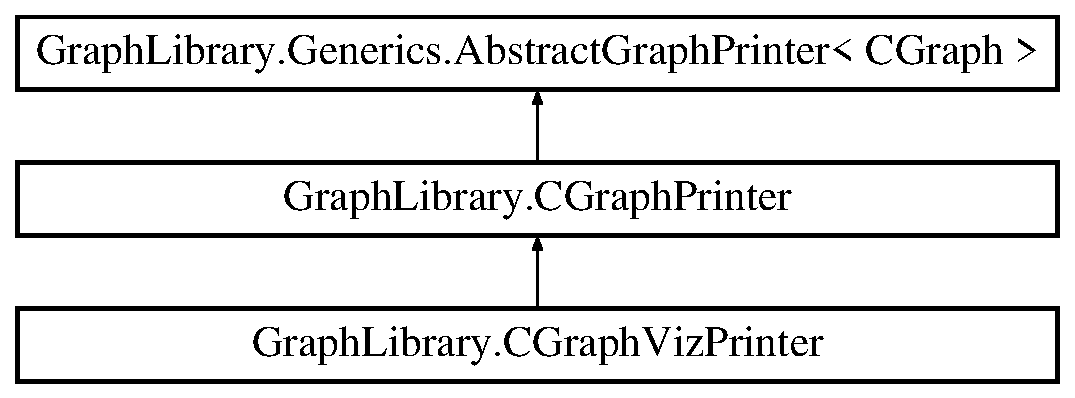
\includegraphics[height=3.000000cm]{class_graph_library_1_1_c_graph_printer}
\end{center}
\end{figure}
\subsection*{Properties}
\begin{DoxyCompactItemize}
\item 
string \hyperlink{class_graph_library_1_1_c_graph_printer_a51fce717e0bd2b68bf8d96f9c6a98b3c}{this\mbox{[}\+C\+Graph\+Node index\mbox{]}}\hspace{0.3cm}{\ttfamily  \mbox{[}get\mbox{]}}
\begin{DoxyCompactList}\small\item\em This indexer facilitates the access to the graph nodes labels. The indexer\textquotesingle{}s type is \hyperlink{class_graph_library_1_1_c_graph_node}{C\+Graph\+Node} and returns the label as a string Gets or sets the System.\+String at the specified index. \end{DoxyCompactList}\end{DoxyCompactItemize}
\subsection*{Additional Inherited Members}


\subsection{Detailed Description}
This class is the parent class of all classes that print \hyperlink{class_graph_library_1_1_c_graph}{C\+Graph} objects Hence the class know the interface of \hyperlink{class_graph_library_1_1_c_graph}{C\+Graph}. (Its build for \hyperlink{class_graph_library_1_1_c_graph}{C\+Graph}). This class heirarchy is based on the Builder design pattern. 



\subsection{Property Documentation}
\hypertarget{class_graph_library_1_1_c_graph_printer_a51fce717e0bd2b68bf8d96f9c6a98b3c}{}\index{Graph\+Library\+::\+C\+Graph\+Printer@{Graph\+Library\+::\+C\+Graph\+Printer}!this\mbox{[}\+C\+Graph\+Node index\mbox{]}@{this[C\+Graph\+Node index]}}
\index{this\mbox{[}\+C\+Graph\+Node index\mbox{]}@{this[C\+Graph\+Node index]}!Graph\+Library\+::\+C\+Graph\+Printer@{Graph\+Library\+::\+C\+Graph\+Printer}}
\subsubsection[{this[C\+Graph\+Node index]}]{\setlength{\rightskip}{0pt plus 5cm}string Graph\+Library.\+C\+Graph\+Printer.\+this\mbox{[}{\bf C\+Graph\+Node} index\mbox{]}\hspace{0.3cm}{\ttfamily [get]}}\label{class_graph_library_1_1_c_graph_printer_a51fce717e0bd2b68bf8d96f9c6a98b3c}


This indexer facilitates the access to the graph nodes labels. The indexer\textquotesingle{}s type is \hyperlink{class_graph_library_1_1_c_graph_node}{C\+Graph\+Node} and returns the label as a string Gets or sets the System.\+String at the specified index. 

The System.\+String. 


\begin{DoxyParams}{Parameters}
{\em index} & The index as \hyperlink{class_graph_library_1_1_c_graph_node}{C\+Graph\+Node} object\\
\hline
\end{DoxyParams}
\begin{DoxyReturn}{Returns}
The label of the node
\end{DoxyReturn}


The documentation for this class was generated from the following file\+:\begin{DoxyCompactItemize}
\item 
Graph\+Library/Graph\+Printers.\+cs\end{DoxyCompactItemize}

\hypertarget{class_graph_library_1_1_c_graph_query_info}{}\section{Graph\+Library.\+C\+Graph\+Query\+Info Class Reference}
\label{class_graph_library_1_1_c_graph_query_info}\index{Graph\+Library.\+C\+Graph\+Query\+Info@{Graph\+Library.\+C\+Graph\+Query\+Info}}


Query info from the \hyperlink{class_graph_library_1_1_c_graph}{C\+Graph} class  


Inheritance diagram for Graph\+Library.\+C\+Graph\+Query\+Info\+:\begin{figure}[H]
\begin{center}
\leavevmode
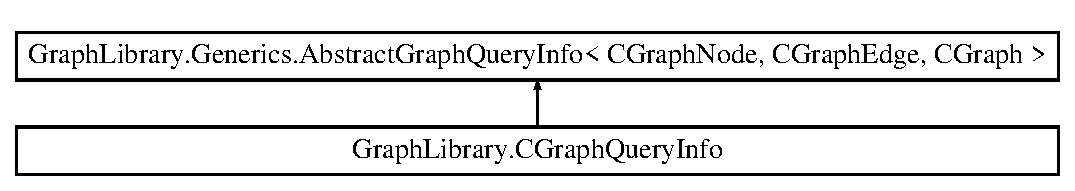
\includegraphics[height=2.000000cm]{class_graph_library_1_1_c_graph_query_info}
\end{center}
\end{figure}
\subsection*{Public Member Functions}
\begin{DoxyCompactItemize}
\item 
\hyperlink{class_graph_library_1_1_c_graph_query_info_a3b4904ea0d850f99d13969b2b060f39b}{C\+Graph\+Query\+Info} (\hyperlink{class_graph_library_1_1_c_graph}{C\+Graph} graph)
\begin{DoxyCompactList}\small\item\em Initializes a new instance of the \hyperlink{class_graph_library_1_1_generics_1_1_abstract_graph_query_info_a8dd567e7f04df4a55df4bd8b4a0c3e48}{Abstract\+Graph\+Query\+Info} class. \end{DoxyCompactList}\item 
override object \hyperlink{class_graph_library_1_1_c_graph_query_info_affa34cf122ba03f978f4a276f32ccfb5}{Info} (\hyperlink{class_graph_library_1_1_c_graph_node}{C\+Graph\+Node} node, object key=null)
\begin{DoxyCompactList}\small\item\em Returns information concerning a node or a graph ( derives from node) Since the graph derives from \hyperlink{class_graph_library_1_1_c_graph_node}{C\+Graph\+Node} it stores the information at the same collection as node. So the function to retrieve the information is common in both elements \end{DoxyCompactList}\item 
override object \hyperlink{class_graph_library_1_1_c_graph_query_info_a0cc7688e9e571af4587c232a51b73acd}{Info} (\hyperlink{class_graph_library_1_1_c_graph_edge}{C\+Graph\+Edge} edge, object key=null)
\begin{DoxyCompactList}\small\item\em Returns the information of the specified edge \end{DoxyCompactList}\item 
override object \hyperlink{class_graph_library_1_1_c_graph_query_info_a1f12d92a287f9f5779416649705f36e4}{Info} (\hyperlink{class_graph_library_1_1_c_graph_node}{C\+Graph\+Node} source, \hyperlink{class_graph_library_1_1_c_graph_node}{C\+Graph\+Node} target, object key=null)
\begin{DoxyCompactList}\small\item\em Returns the information of the edge between the given source and target nodes. \end{DoxyCompactList}\item 
override object \hyperlink{class_graph_library_1_1_c_graph_query_info_adc1215f254e82c2dfee52279b49bba64}{Create\+Info} (\hyperlink{class_graph_library_1_1_c_graph_node}{C\+Graph\+Node} node, object info, object key=null)
\begin{DoxyCompactList}\small\item\em Stores the information at the specified node or graph. If information already exists, it is overwritten \end{DoxyCompactList}\item 
override object \hyperlink{class_graph_library_1_1_c_graph_query_info_a7b0cf74374283e88bf6309acb1c63a2c}{Create\+Info} (\hyperlink{class_graph_library_1_1_c_graph_edge}{C\+Graph\+Edge} edge, object info, object key=null)
\begin{DoxyCompactList}\small\item\em Stores the information at the specified edge. If information already exists, it is overwritten \end{DoxyCompactList}\item 
override object \hyperlink{class_graph_library_1_1_c_graph_query_info_ab7bfe088c7bad560bf15784468f6eb2a}{Create\+Info} (\hyperlink{class_graph_library_1_1_c_graph_node}{C\+Graph\+Node} source, \hyperlink{class_graph_library_1_1_c_graph_node}{C\+Graph\+Node} target, object info, object key=null)
\begin{DoxyCompactList}\small\item\em Stores the information at the specified edge. If information already exists, it is overwritten \end{DoxyCompactList}\end{DoxyCompactItemize}
\subsection*{Additional Inherited Members}


\subsection{Detailed Description}
Query info from the \hyperlink{class_graph_library_1_1_c_graph}{C\+Graph} class 

\begin{DoxySeeAlso}{See also}
Graph\+Library.\+Abstract\+Graph\+Query\+Info$<$\+Graph\+Library.\+C\+Graph\+Node,\+Graph\+Library.\+C\+Graph\+Edge,\+Graph\+Library.\+C\+Graph$>$


\end{DoxySeeAlso}


\subsection{Constructor \& Destructor Documentation}
\hypertarget{class_graph_library_1_1_c_graph_query_info_a3b4904ea0d850f99d13969b2b060f39b}{}\index{Graph\+Library\+::\+C\+Graph\+Query\+Info@{Graph\+Library\+::\+C\+Graph\+Query\+Info}!C\+Graph\+Query\+Info@{C\+Graph\+Query\+Info}}
\index{C\+Graph\+Query\+Info@{C\+Graph\+Query\+Info}!Graph\+Library\+::\+C\+Graph\+Query\+Info@{Graph\+Library\+::\+C\+Graph\+Query\+Info}}
\subsubsection[{C\+Graph\+Query\+Info(\+C\+Graph graph)}]{\setlength{\rightskip}{0pt plus 5cm}Graph\+Library.\+C\+Graph\+Query\+Info.\+C\+Graph\+Query\+Info (
\begin{DoxyParamCaption}
\item[{{\bf C\+Graph}}]{graph}
\end{DoxyParamCaption}
)}\label{class_graph_library_1_1_c_graph_query_info_a3b4904ea0d850f99d13969b2b060f39b}


Initializes a new instance of the \hyperlink{class_graph_library_1_1_generics_1_1_abstract_graph_query_info_a8dd567e7f04df4a55df4bd8b4a0c3e48}{Abstract\+Graph\+Query\+Info} class. 


\begin{DoxyParams}{Parameters}
{\em graph} & The graph.\\
\hline
\end{DoxyParams}


\subsection{Member Function Documentation}
\hypertarget{class_graph_library_1_1_c_graph_query_info_adc1215f254e82c2dfee52279b49bba64}{}\index{Graph\+Library\+::\+C\+Graph\+Query\+Info@{Graph\+Library\+::\+C\+Graph\+Query\+Info}!Create\+Info@{Create\+Info}}
\index{Create\+Info@{Create\+Info}!Graph\+Library\+::\+C\+Graph\+Query\+Info@{Graph\+Library\+::\+C\+Graph\+Query\+Info}}
\subsubsection[{Create\+Info(\+C\+Graph\+Node node, object info, object key=null)}]{\setlength{\rightskip}{0pt plus 5cm}override object Graph\+Library.\+C\+Graph\+Query\+Info.\+Create\+Info (
\begin{DoxyParamCaption}
\item[{{\bf C\+Graph\+Node}}]{node, }
\item[{object}]{info, }
\item[{object}]{key = {\ttfamily null}}
\end{DoxyParamCaption}
)}\label{class_graph_library_1_1_c_graph_query_info_adc1215f254e82c2dfee52279b49bba64}


Stores the information at the specified node or graph. If information already exists, it is overwritten 


\begin{DoxyParams}{Parameters}
{\em node} & The node.\\
\hline
{\em info} & The information.\\
\hline
{\em key} & The key that will extract the information from the specified node\textquotesingle{}s dictionary. If null is given then the current Query Info object is used as a key. Thus the Query\+Info object can be used as an information creator/exploitator\\
\hline
\end{DoxyParams}
\begin{DoxyReturn}{Returns}
The information object 
\end{DoxyReturn}
\hypertarget{class_graph_library_1_1_c_graph_query_info_a7b0cf74374283e88bf6309acb1c63a2c}{}\index{Graph\+Library\+::\+C\+Graph\+Query\+Info@{Graph\+Library\+::\+C\+Graph\+Query\+Info}!Create\+Info@{Create\+Info}}
\index{Create\+Info@{Create\+Info}!Graph\+Library\+::\+C\+Graph\+Query\+Info@{Graph\+Library\+::\+C\+Graph\+Query\+Info}}
\subsubsection[{Create\+Info(\+C\+Graph\+Edge edge, object info, object key=null)}]{\setlength{\rightskip}{0pt plus 5cm}override object Graph\+Library.\+C\+Graph\+Query\+Info.\+Create\+Info (
\begin{DoxyParamCaption}
\item[{{\bf C\+Graph\+Edge}}]{edge, }
\item[{object}]{info, }
\item[{object}]{key = {\ttfamily null}}
\end{DoxyParamCaption}
)}\label{class_graph_library_1_1_c_graph_query_info_a7b0cf74374283e88bf6309acb1c63a2c}


Stores the information at the specified edge. If information already exists, it is overwritten 


\begin{DoxyParams}{Parameters}
{\em edge} & The edge.\\
\hline
{\em info} & The information object.\\
\hline
{\em key} & The key that will extract the information from the specified node\textquotesingle{}s dictionary. If null is given then the current Query Info object is used as a key\\
\hline
\end{DoxyParams}
\begin{DoxyReturn}{Returns}
The information object 
\end{DoxyReturn}
\hypertarget{class_graph_library_1_1_c_graph_query_info_ab7bfe088c7bad560bf15784468f6eb2a}{}\index{Graph\+Library\+::\+C\+Graph\+Query\+Info@{Graph\+Library\+::\+C\+Graph\+Query\+Info}!Create\+Info@{Create\+Info}}
\index{Create\+Info@{Create\+Info}!Graph\+Library\+::\+C\+Graph\+Query\+Info@{Graph\+Library\+::\+C\+Graph\+Query\+Info}}
\subsubsection[{Create\+Info(\+C\+Graph\+Node source, C\+Graph\+Node target, object info, object key=null)}]{\setlength{\rightskip}{0pt plus 5cm}override object Graph\+Library.\+C\+Graph\+Query\+Info.\+Create\+Info (
\begin{DoxyParamCaption}
\item[{{\bf C\+Graph\+Node}}]{source, }
\item[{{\bf C\+Graph\+Node}}]{target, }
\item[{object}]{info, }
\item[{object}]{key = {\ttfamily null}}
\end{DoxyParamCaption}
)}\label{class_graph_library_1_1_c_graph_query_info_ab7bfe088c7bad560bf15784468f6eb2a}


Stores the information at the specified edge. If information already exists, it is overwritten 


\begin{DoxyParams}{Parameters}
{\em source} & The source node.\\
\hline
{\em target} & The target node.\\
\hline
{\em info} & The information.\\
\hline
{\em key} & The key that will extract the information from the specified node\textquotesingle{}s dictionary. If null is given then the current Query Info object is used as a key\\
\hline
\end{DoxyParams}
\begin{DoxyReturn}{Returns}
The information object 
\end{DoxyReturn}
\hypertarget{class_graph_library_1_1_c_graph_query_info_affa34cf122ba03f978f4a276f32ccfb5}{}\index{Graph\+Library\+::\+C\+Graph\+Query\+Info@{Graph\+Library\+::\+C\+Graph\+Query\+Info}!Info@{Info}}
\index{Info@{Info}!Graph\+Library\+::\+C\+Graph\+Query\+Info@{Graph\+Library\+::\+C\+Graph\+Query\+Info}}
\subsubsection[{Info(\+C\+Graph\+Node node, object key=null)}]{\setlength{\rightskip}{0pt plus 5cm}override object Graph\+Library.\+C\+Graph\+Query\+Info.\+Info (
\begin{DoxyParamCaption}
\item[{{\bf C\+Graph\+Node}}]{node, }
\item[{object}]{key = {\ttfamily null}}
\end{DoxyParamCaption}
)}\label{class_graph_library_1_1_c_graph_query_info_affa34cf122ba03f978f4a276f32ccfb5}


Returns information concerning a node or a graph ( derives from node) Since the graph derives from \hyperlink{class_graph_library_1_1_c_graph_node}{C\+Graph\+Node} it stores the information at the same collection as node. So the function to retrieve the information is common in both elements 


\begin{DoxyParams}{Parameters}
{\em node} & The node.\\
\hline
{\em key} & The key that will extract the information from the specified node\textquotesingle{}s dictionary. If null is given then the current Query Info object is used as a key\\
\hline
\end{DoxyParams}
\begin{DoxyReturn}{Returns}

\end{DoxyReturn}
\hypertarget{class_graph_library_1_1_c_graph_query_info_a0cc7688e9e571af4587c232a51b73acd}{}\index{Graph\+Library\+::\+C\+Graph\+Query\+Info@{Graph\+Library\+::\+C\+Graph\+Query\+Info}!Info@{Info}}
\index{Info@{Info}!Graph\+Library\+::\+C\+Graph\+Query\+Info@{Graph\+Library\+::\+C\+Graph\+Query\+Info}}
\subsubsection[{Info(\+C\+Graph\+Edge edge, object key=null)}]{\setlength{\rightskip}{0pt plus 5cm}override object Graph\+Library.\+C\+Graph\+Query\+Info.\+Info (
\begin{DoxyParamCaption}
\item[{{\bf C\+Graph\+Edge}}]{edge, }
\item[{object}]{key = {\ttfamily null}}
\end{DoxyParamCaption}
)}\label{class_graph_library_1_1_c_graph_query_info_a0cc7688e9e571af4587c232a51b73acd}


Returns the information of the specified edge 


\begin{DoxyParams}{Parameters}
{\em edge} & The edge.\\
\hline
{\em key} & The key that will extract the information from the specified node\textquotesingle{}s dictionary. If null is given then the current Query Info object is used as a key\\
\hline
\end{DoxyParams}
\begin{DoxyReturn}{Returns}

\end{DoxyReturn}
\hypertarget{class_graph_library_1_1_c_graph_query_info_a1f12d92a287f9f5779416649705f36e4}{}\index{Graph\+Library\+::\+C\+Graph\+Query\+Info@{Graph\+Library\+::\+C\+Graph\+Query\+Info}!Info@{Info}}
\index{Info@{Info}!Graph\+Library\+::\+C\+Graph\+Query\+Info@{Graph\+Library\+::\+C\+Graph\+Query\+Info}}
\subsubsection[{Info(\+C\+Graph\+Node source, C\+Graph\+Node target, object key=null)}]{\setlength{\rightskip}{0pt plus 5cm}override object Graph\+Library.\+C\+Graph\+Query\+Info.\+Info (
\begin{DoxyParamCaption}
\item[{{\bf C\+Graph\+Node}}]{source, }
\item[{{\bf C\+Graph\+Node}}]{target, }
\item[{object}]{key = {\ttfamily null}}
\end{DoxyParamCaption}
)}\label{class_graph_library_1_1_c_graph_query_info_a1f12d92a287f9f5779416649705f36e4}


Returns the information of the edge between the given source and target nodes. 


\begin{DoxyParams}{Parameters}
{\em source} & The source.\\
\hline
{\em target} & The target.\\
\hline
{\em key} & The key that will extract the information from the specified node\textquotesingle{}s dictionary.\+If null is given then the current Query Info object is used as a key\\
\hline
\end{DoxyParams}
\begin{DoxyReturn}{Returns}

\end{DoxyReturn}


The documentation for this class was generated from the following file\+:\begin{DoxyCompactItemize}
\item 
Graph\+Library/Graph\+Query\+Info.\+cs\end{DoxyCompactItemize}

\hypertarget{class_graph_library_1_1_c_graph_viz_printer}{}\section{Graph\+Library.\+C\+Graph\+Viz\+Printer Class Reference}
\label{class_graph_library_1_1_c_graph_viz_printer}\index{Graph\+Library.\+C\+Graph\+Viz\+Printer@{Graph\+Library.\+C\+Graph\+Viz\+Printer}}


This class exports the graph in graphviz form. It accepts the graph and optionally a class that defined the labelling of nodes. If the client doen\textquotesingle{}t provide a labelling class a default class (Graph\+Viz\+Node\+Labeling) takes over the labelling of nodes  


Inheritance diagram for Graph\+Library.\+C\+Graph\+Viz\+Printer\+:\begin{figure}[H]
\begin{center}
\leavevmode
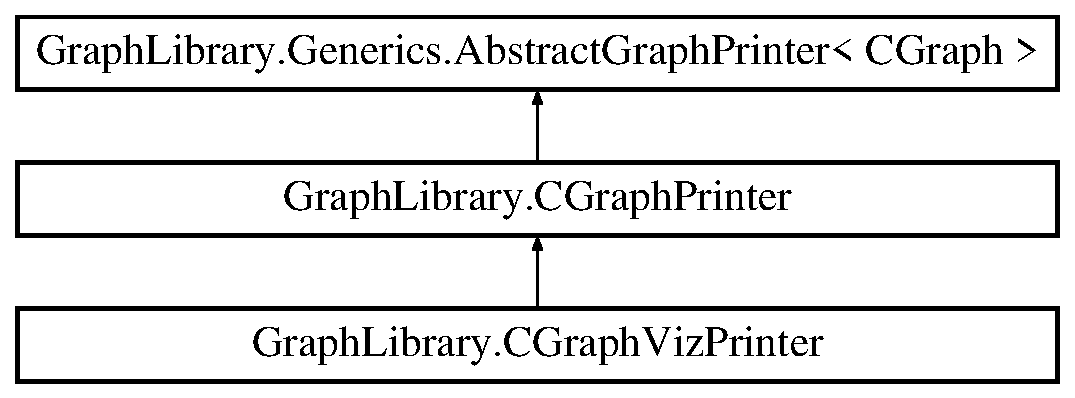
\includegraphics[height=3.000000cm]{class_graph_library_1_1_c_graph_viz_printer}
\end{center}
\end{figure}
\subsection*{Public Member Functions}
\begin{DoxyCompactItemize}
\item 
\hypertarget{class_graph_library_1_1_c_graph_viz_printer_abb31a40f8b3a16c8abe21ca13d4debb0}{}{\bfseries C\+Graph\+Viz\+Printer} (\hyperlink{class_graph_library_1_1_c_graph}{C\+Graph} graph, \hyperlink{class_graph_library_1_1_c_graph_labeling}{C\+Graph\+Labeling}$<$ \hyperlink{class_graph_library_1_1_c_graph_node}{C\+Graph\+Node} $>$ labeling=null)\label{class_graph_library_1_1_c_graph_viz_printer_abb31a40f8b3a16c8abe21ca13d4debb0}

\item 
override String\+Builder \hyperlink{class_graph_library_1_1_c_graph_viz_printer_a5341d69647f313d81387578a629d1ed5}{Print} (bool onlyedges=false)
\begin{DoxyCompactList}\small\item\em Prints the graph into a String\+Builder object. Optionally the header and footer of the .dot file can be ommited for use of the graph edges in the multi layer graph printer \end{DoxyCompactList}\item 
override void \hyperlink{class_graph_library_1_1_c_graph_viz_printer_a9d4366ecf1b1f27c8886f0891ae5f5cf}{Generate} (string filepath, bool execute\+Generator=true)
\begin{DoxyCompactList}\small\item\em Generates the Graph\+Viz .dot file and optionally calls the graphviz to generate the picture of the graph. \end{DoxyCompactList}\end{DoxyCompactItemize}
\subsection*{Additional Inherited Members}


\subsection{Detailed Description}
This class exports the graph in graphviz form. It accepts the graph and optionally a class that defined the labelling of nodes. If the client doen\textquotesingle{}t provide a labelling class a default class (Graph\+Viz\+Node\+Labeling) takes over the labelling of nodes 

\begin{DoxySeeAlso}{See also}
\hyperlink{class_graph_library_1_1_c_graph_printer}{Graph\+Library.\+C\+Graph\+Printer}


\end{DoxySeeAlso}


\subsection{Member Function Documentation}
\hypertarget{class_graph_library_1_1_c_graph_viz_printer_a9d4366ecf1b1f27c8886f0891ae5f5cf}{}\index{Graph\+Library\+::\+C\+Graph\+Viz\+Printer@{Graph\+Library\+::\+C\+Graph\+Viz\+Printer}!Generate@{Generate}}
\index{Generate@{Generate}!Graph\+Library\+::\+C\+Graph\+Viz\+Printer@{Graph\+Library\+::\+C\+Graph\+Viz\+Printer}}
\subsubsection[{Generate(string filepath, bool execute\+Generator=true)}]{\setlength{\rightskip}{0pt plus 5cm}override void Graph\+Library.\+C\+Graph\+Viz\+Printer.\+Generate (
\begin{DoxyParamCaption}
\item[{string}]{filepath, }
\item[{bool}]{execute\+Generator = {\ttfamily true}}
\end{DoxyParamCaption}
)\hspace{0.3cm}{\ttfamily [virtual]}}\label{class_graph_library_1_1_c_graph_viz_printer_a9d4366ecf1b1f27c8886f0891ae5f5cf}


Generates the Graph\+Viz .dot file and optionally calls the graphviz to generate the picture of the graph. 


\begin{DoxyParams}{Parameters}
{\em filepath} & The full path to which the file is generated\\
\hline
{\em execute\+Generator} & If true calls the dot tool to produce the graph in a picture\\
\hline
\end{DoxyParams}


Implements \hyperlink{class_graph_library_1_1_generics_1_1_abstract_graph_printer_ae58857c9c21ef8ab2cd8a0651340e2ec}{Graph\+Library.\+Generics.\+Abstract\+Graph\+Printer$<$ C\+Graph $>$}.

\hypertarget{class_graph_library_1_1_c_graph_viz_printer_a5341d69647f313d81387578a629d1ed5}{}\index{Graph\+Library\+::\+C\+Graph\+Viz\+Printer@{Graph\+Library\+::\+C\+Graph\+Viz\+Printer}!Print@{Print}}
\index{Print@{Print}!Graph\+Library\+::\+C\+Graph\+Viz\+Printer@{Graph\+Library\+::\+C\+Graph\+Viz\+Printer}}
\subsubsection[{Print(bool onlyedges=false)}]{\setlength{\rightskip}{0pt plus 5cm}override String\+Builder Graph\+Library.\+C\+Graph\+Viz\+Printer.\+Print (
\begin{DoxyParamCaption}
\item[{bool}]{onlyedges = {\ttfamily false}}
\end{DoxyParamCaption}
)\hspace{0.3cm}{\ttfamily [virtual]}}\label{class_graph_library_1_1_c_graph_viz_printer_a5341d69647f313d81387578a629d1ed5}


Prints the graph into a String\+Builder object. Optionally the header and footer of the .dot file can be ommited for use of the graph edges in the multi layer graph printer 


\begin{DoxyParams}{Parameters}
{\em onlyedges} & if set to {\ttfamily true} \mbox{[}onlyedges\mbox{]}.\\
\hline
\end{DoxyParams}
\begin{DoxyReturn}{Returns}

\end{DoxyReturn}

\begin{DoxyExceptions}{Exceptions}
{\em System.\+Not\+Implemented\+Exception} & \\
\hline
\end{DoxyExceptions}


Implements \hyperlink{class_graph_library_1_1_generics_1_1_abstract_graph_printer_a793fd0ab2baf6809eee04292d3992ce4}{Graph\+Library.\+Generics.\+Abstract\+Graph\+Printer$<$ C\+Graph $>$}.



The documentation for this class was generated from the following file\+:\begin{DoxyCompactItemize}
\item 
Graph\+Library/\+Printers/\+Graph\+Viz\+Printer/Graph\+Viz\+Printer.\+cs\end{DoxyCompactItemize}

\hypertarget{class_graph_library_1_1_c_it___graph_b_f_s}{}\section{Graph\+Library.\+C\+It\+\_\+\+Graph\+B\+F\+S Class Reference}
\label{class_graph_library_1_1_c_it___graph_b_f_s}\index{Graph\+Library.\+C\+It\+\_\+\+Graph\+B\+F\+S@{Graph\+Library.\+C\+It\+\_\+\+Graph\+B\+F\+S}}


Iterates over the nodes of a graph using Breadth First Traversal The graph can be directed or undirected  


Inheritance diagram for Graph\+Library.\+C\+It\+\_\+\+Graph\+B\+F\+S\+:\begin{figure}[H]
\begin{center}
\leavevmode
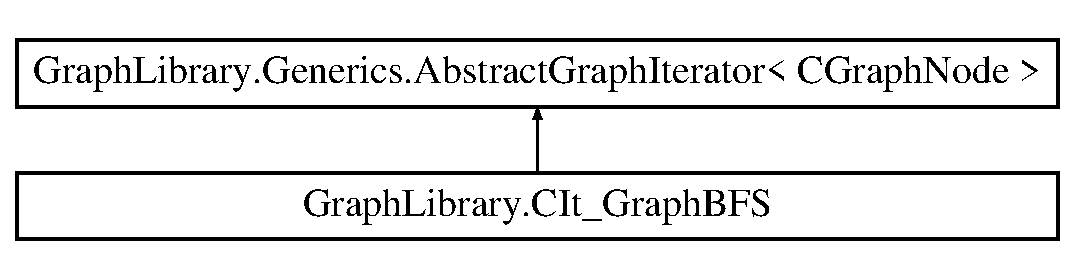
\includegraphics[height=2.000000cm]{class_graph_library_1_1_c_it___graph_b_f_s}
\end{center}
\end{figure}
\subsection*{Classes}
\begin{DoxyCompactItemize}
\item 
class \hyperlink{class_graph_library_1_1_c_it___graph_b_f_s_1_1_info___d_f_s}{Info\+\_\+\+D\+F\+S}
\begin{DoxyCompactList}\small\item\em Graph node info to assist the iterator algorithm \end{DoxyCompactList}\end{DoxyCompactItemize}
\subsection*{Public Member Functions}
\begin{DoxyCompactItemize}
\item 
\hypertarget{class_graph_library_1_1_c_it___graph_b_f_s_a2d8f7a4ef8361ac7d0093db4be305169}{}{\bfseries C\+It\+\_\+\+Graph\+B\+F\+S} (\hyperlink{class_graph_library_1_1_c_graph}{C\+Graph} m\+Graph, \hyperlink{class_graph_library_1_1_c_graph_node}{C\+Graph\+Node} start\+Node)\label{class_graph_library_1_1_c_it___graph_b_f_s_a2d8f7a4ef8361ac7d0093db4be305169}

\item 
override \hyperlink{class_graph_library_1_1_c_graph_node}{C\+Graph\+Node} \hyperlink{class_graph_library_1_1_c_it___graph_b_f_s_aa96b96be6229e08e45b85fcd0130445d}{Begin} ()
\begin{DoxyCompactList}\small\item\em Executes once at the start of the iteration and before the \hyperlink{class_graph_library_1_1_c_it___graph_b_f_s_a46418dc24ecf2e8ad3aa3541a70d06b2}{End()} method Initializes the iterator variable ( realized in the subclasses ) and the m\+\_\+current\+Item to point to the first element of the item set. If the set is empty the m\+\_\+current\+Item points to null. After the \hyperlink{class_graph_library_1_1_c_it___graph_b_f_s_aa96b96be6229e08e45b85fcd0130445d}{Begin()} method the \hyperlink{class_graph_library_1_1_c_it___graph_b_f_s_a46418dc24ecf2e8ad3aa3541a70d06b2}{End()} method executes before going into the loop body. Thus the loop terminates if the item set is empty before ever running the loop body The transition logic for finding the first item in the items set is implemented in the subclasses \end{DoxyCompactList}\item 
override bool \hyperlink{class_graph_library_1_1_c_it___graph_b_f_s_a46418dc24ecf2e8ad3aa3541a70d06b2}{End} ()
\begin{DoxyCompactList}\small\item\em Executes after the \hyperlink{class_graph_library_1_1_c_it___graph_b_f_s_aa96b96be6229e08e45b85fcd0130445d}{Begin()} or \hyperlink{class_graph_library_1_1_c_it___graph_b_f_s_ab836a3c5caca3c8d63d56827b677a243}{Next()} methods and before the Loop Body Returns true if the m\+\_\+current\+Item is null. This case arises in the following scenarios\+: 1) The item set is empty thus, after the \hyperlink{class_graph_library_1_1_c_it___graph_b_f_s_aa96b96be6229e08e45b85fcd0130445d}{Begin()} method call the \hyperlink{class_graph_library_1_1_c_it___graph_b_f_s_a46418dc24ecf2e8ad3aa3541a70d06b2}{End()} identifies that m\+\_\+current\+Item points to null 2) The item set is not empty and the iterator went outside the boundaries of the item set after the call to \hyperlink{class_graph_library_1_1_c_it___graph_b_f_s_ab836a3c5caca3c8d63d56827b677a243}{Next()} method (\hyperlink{class_graph_library_1_1_c_it___graph_b_f_s_ab836a3c5caca3c8d63d56827b677a243}{Next()} method set m\+\_\+current\+Item to null) \end{DoxyCompactList}\item 
override \hyperlink{class_graph_library_1_1_c_graph_node}{C\+Graph\+Node} \hyperlink{class_graph_library_1_1_c_it___graph_b_f_s_ab836a3c5caca3c8d63d56827b677a243}{Next} ()
\begin{DoxyCompactList}\small\item\em Executes after the execution of the loop body and before the \hyperlink{class_graph_library_1_1_c_it___graph_b_f_s_a46418dc24ecf2e8ad3aa3541a70d06b2}{End()} method Increases the iteration variable and set the m\+\_\+current\+Item to point to the current item of the item set. In case where the end of the item set is reached the m\+\_\+current\+Item points to null which is identified by the \hyperlink{class_graph_library_1_1_c_it___graph_b_f_s_a46418dc24ecf2e8ad3aa3541a70d06b2}{End()} methods that is executed next. The transition logic from item to item is implemented from the subclasses. \end{DoxyCompactList}\end{DoxyCompactItemize}
\subsection*{Protected Member Functions}
\begin{DoxyCompactItemize}
\item 
\hypertarget{class_graph_library_1_1_c_it___graph_b_f_s_a23f45ca6cd30441e3204f269a01f6c66}{}void {\bfseries Set\+Node\+Color} (\hyperlink{class_graph_library_1_1_c_graph_node}{C\+Graph\+Node} node, int color)\label{class_graph_library_1_1_c_it___graph_b_f_s_a23f45ca6cd30441e3204f269a01f6c66}

\item 
\hypertarget{class_graph_library_1_1_c_it___graph_b_f_s_a1c08c6b1ae81ac9599844f7269de5a38}{}int {\bfseries Get\+Node\+Color} (\hyperlink{class_graph_library_1_1_c_graph_node}{C\+Graph\+Node} node)\label{class_graph_library_1_1_c_it___graph_b_f_s_a1c08c6b1ae81ac9599844f7269de5a38}

\item 
\hypertarget{class_graph_library_1_1_c_it___graph_b_f_s_ae3bf125e1855a8a4dbf751bce31fd138}{}void {\bfseries Set\+Node\+Distance} (\hyperlink{class_graph_library_1_1_c_graph_node}{C\+Graph\+Node} node, int distance)\label{class_graph_library_1_1_c_it___graph_b_f_s_ae3bf125e1855a8a4dbf751bce31fd138}

\item 
\hypertarget{class_graph_library_1_1_c_it___graph_b_f_s_a13899ef9bfec0a8da8248b06946d0f8f}{}int {\bfseries Get\+Node\+Distance} (\hyperlink{class_graph_library_1_1_c_graph_node}{C\+Graph\+Node} node)\label{class_graph_library_1_1_c_it___graph_b_f_s_a13899ef9bfec0a8da8248b06946d0f8f}

\end{DoxyCompactItemize}
\subsection*{Protected Attributes}
\begin{DoxyCompactItemize}
\item 
\hypertarget{class_graph_library_1_1_c_it___graph_b_f_s_adacf8b394fdb6568c5c0de07947800db}{}Queue$<$ \hyperlink{class_graph_library_1_1_c_graph_node}{C\+Graph\+Node} $>$ {\bfseries m\+\_\+queue}\label{class_graph_library_1_1_c_it___graph_b_f_s_adacf8b394fdb6568c5c0de07947800db}

\end{DoxyCompactItemize}
\subsection*{Additional Inherited Members}


\subsection{Detailed Description}
Iterates over the nodes of a graph using Breadth First Traversal The graph can be directed or undirected 



\subsection{Member Function Documentation}
\hypertarget{class_graph_library_1_1_c_it___graph_b_f_s_aa96b96be6229e08e45b85fcd0130445d}{}\index{Graph\+Library\+::\+C\+It\+\_\+\+Graph\+B\+F\+S@{Graph\+Library\+::\+C\+It\+\_\+\+Graph\+B\+F\+S}!Begin@{Begin}}
\index{Begin@{Begin}!Graph\+Library\+::\+C\+It\+\_\+\+Graph\+B\+F\+S@{Graph\+Library\+::\+C\+It\+\_\+\+Graph\+B\+F\+S}}
\subsubsection[{Begin()}]{\setlength{\rightskip}{0pt plus 5cm}override {\bf C\+Graph\+Node} Graph\+Library.\+C\+It\+\_\+\+Graph\+B\+F\+S.\+Begin (
\begin{DoxyParamCaption}
{}
\end{DoxyParamCaption}
)\hspace{0.3cm}{\ttfamily [virtual]}}\label{class_graph_library_1_1_c_it___graph_b_f_s_aa96b96be6229e08e45b85fcd0130445d}


Executes once at the start of the iteration and before the \hyperlink{class_graph_library_1_1_c_it___graph_b_f_s_a46418dc24ecf2e8ad3aa3541a70d06b2}{End()} method Initializes the iterator variable ( realized in the subclasses ) and the m\+\_\+current\+Item to point to the first element of the item set. If the set is empty the m\+\_\+current\+Item points to null. After the \hyperlink{class_graph_library_1_1_c_it___graph_b_f_s_aa96b96be6229e08e45b85fcd0130445d}{Begin()} method the \hyperlink{class_graph_library_1_1_c_it___graph_b_f_s_a46418dc24ecf2e8ad3aa3541a70d06b2}{End()} method executes before going into the loop body. Thus the loop terminates if the item set is empty before ever running the loop body The transition logic for finding the first item in the items set is implemented in the subclasses 

\begin{DoxyReturn}{Returns}

\end{DoxyReturn}


Implements \hyperlink{class_graph_library_1_1_generics_1_1_abstract_graph_iterator_a2c97c7a412c233b8442b7ad403f29779}{Graph\+Library.\+Generics.\+Abstract\+Graph\+Iterator$<$ C\+Graph\+Node $>$}.

\hypertarget{class_graph_library_1_1_c_it___graph_b_f_s_a46418dc24ecf2e8ad3aa3541a70d06b2}{}\index{Graph\+Library\+::\+C\+It\+\_\+\+Graph\+B\+F\+S@{Graph\+Library\+::\+C\+It\+\_\+\+Graph\+B\+F\+S}!End@{End}}
\index{End@{End}!Graph\+Library\+::\+C\+It\+\_\+\+Graph\+B\+F\+S@{Graph\+Library\+::\+C\+It\+\_\+\+Graph\+B\+F\+S}}
\subsubsection[{End()}]{\setlength{\rightskip}{0pt plus 5cm}override bool Graph\+Library.\+C\+It\+\_\+\+Graph\+B\+F\+S.\+End (
\begin{DoxyParamCaption}
{}
\end{DoxyParamCaption}
)\hspace{0.3cm}{\ttfamily [virtual]}}\label{class_graph_library_1_1_c_it___graph_b_f_s_a46418dc24ecf2e8ad3aa3541a70d06b2}


Executes after the \hyperlink{class_graph_library_1_1_c_it___graph_b_f_s_aa96b96be6229e08e45b85fcd0130445d}{Begin()} or \hyperlink{class_graph_library_1_1_c_it___graph_b_f_s_ab836a3c5caca3c8d63d56827b677a243}{Next()} methods and before the Loop Body Returns true if the m\+\_\+current\+Item is null. This case arises in the following scenarios\+: 1) The item set is empty thus, after the \hyperlink{class_graph_library_1_1_c_it___graph_b_f_s_aa96b96be6229e08e45b85fcd0130445d}{Begin()} method call the \hyperlink{class_graph_library_1_1_c_it___graph_b_f_s_a46418dc24ecf2e8ad3aa3541a70d06b2}{End()} identifies that m\+\_\+current\+Item points to null 2) The item set is not empty and the iterator went outside the boundaries of the item set after the call to \hyperlink{class_graph_library_1_1_c_it___graph_b_f_s_ab836a3c5caca3c8d63d56827b677a243}{Next()} method (\hyperlink{class_graph_library_1_1_c_it___graph_b_f_s_ab836a3c5caca3c8d63d56827b677a243}{Next()} method set m\+\_\+current\+Item to null) 

\begin{DoxyReturn}{Returns}

\end{DoxyReturn}


Implements \hyperlink{class_graph_library_1_1_generics_1_1_abstract_graph_iterator_aa8cd9f596ec0b6c4c1e9c244ba75df04}{Graph\+Library.\+Generics.\+Abstract\+Graph\+Iterator$<$ C\+Graph\+Node $>$}.

\hypertarget{class_graph_library_1_1_c_it___graph_b_f_s_ab836a3c5caca3c8d63d56827b677a243}{}\index{Graph\+Library\+::\+C\+It\+\_\+\+Graph\+B\+F\+S@{Graph\+Library\+::\+C\+It\+\_\+\+Graph\+B\+F\+S}!Next@{Next}}
\index{Next@{Next}!Graph\+Library\+::\+C\+It\+\_\+\+Graph\+B\+F\+S@{Graph\+Library\+::\+C\+It\+\_\+\+Graph\+B\+F\+S}}
\subsubsection[{Next()}]{\setlength{\rightskip}{0pt plus 5cm}override {\bf C\+Graph\+Node} Graph\+Library.\+C\+It\+\_\+\+Graph\+B\+F\+S.\+Next (
\begin{DoxyParamCaption}
{}
\end{DoxyParamCaption}
)\hspace{0.3cm}{\ttfamily [virtual]}}\label{class_graph_library_1_1_c_it___graph_b_f_s_ab836a3c5caca3c8d63d56827b677a243}


Executes after the execution of the loop body and before the \hyperlink{class_graph_library_1_1_c_it___graph_b_f_s_a46418dc24ecf2e8ad3aa3541a70d06b2}{End()} method Increases the iteration variable and set the m\+\_\+current\+Item to point to the current item of the item set. In case where the end of the item set is reached the m\+\_\+current\+Item points to null which is identified by the \hyperlink{class_graph_library_1_1_c_it___graph_b_f_s_a46418dc24ecf2e8ad3aa3541a70d06b2}{End()} methods that is executed next. The transition logic from item to item is implemented from the subclasses. 

\begin{DoxyReturn}{Returns}

\end{DoxyReturn}


Implements \hyperlink{class_graph_library_1_1_generics_1_1_abstract_graph_iterator_aac8cffd0d579708a94ba056e4f4a00b2}{Graph\+Library.\+Generics.\+Abstract\+Graph\+Iterator$<$ C\+Graph\+Node $>$}.



The documentation for this class was generated from the following file\+:\begin{DoxyCompactItemize}
\item 
Graph\+Library/Graph\+Iterators.\+cs\end{DoxyCompactItemize}

\hypertarget{class_graph_library_1_1_c_it___graph_d_f_s}{}\section{Graph\+Library.\+C\+It\+\_\+\+Graph\+D\+F\+S Class Reference}
\label{class_graph_library_1_1_c_it___graph_d_f_s}\index{Graph\+Library.\+C\+It\+\_\+\+Graph\+D\+F\+S@{Graph\+Library.\+C\+It\+\_\+\+Graph\+D\+F\+S}}


Iterates over the nodes of a graph using Depth First Traversal The graph can be directed or undirected  


Inheritance diagram for Graph\+Library.\+C\+It\+\_\+\+Graph\+D\+F\+S\+:\begin{figure}[H]
\begin{center}
\leavevmode
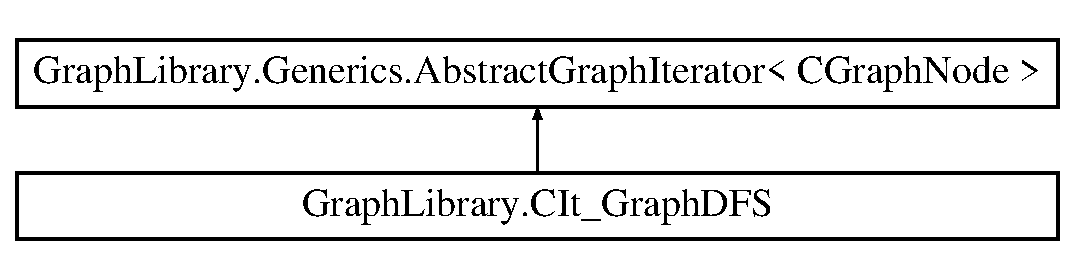
\includegraphics[height=2.000000cm]{class_graph_library_1_1_c_it___graph_d_f_s}
\end{center}
\end{figure}
\subsection*{Classes}
\begin{DoxyCompactItemize}
\item 
class \hyperlink{class_graph_library_1_1_c_it___graph_d_f_s_1_1_info___d_f_s}{Info\+\_\+\+D\+F\+S}
\begin{DoxyCompactList}\small\item\em Graph node info to assist the iterator algorithm \end{DoxyCompactList}\end{DoxyCompactItemize}
\subsection*{Public Member Functions}
\begin{DoxyCompactItemize}
\item 
\hypertarget{class_graph_library_1_1_c_it___graph_d_f_s_afbed060eff3b2fbf3056e6bbb635c976}{}{\bfseries C\+It\+\_\+\+Graph\+D\+F\+S} (\hyperlink{class_graph_library_1_1_c_graph}{C\+Graph} m\+Graph)\label{class_graph_library_1_1_c_it___graph_d_f_s_afbed060eff3b2fbf3056e6bbb635c976}

\item 
override \hyperlink{class_graph_library_1_1_c_graph_node}{C\+Graph\+Node} \hyperlink{class_graph_library_1_1_c_it___graph_d_f_s_a0c5f16a80d9647af3bf1ad35507fe62a}{Begin} ()
\begin{DoxyCompactList}\small\item\em Executes once at the start of the iteration and before the \hyperlink{class_graph_library_1_1_c_it___graph_d_f_s_a6f6992493bc70c2e551c5d46bf9bf998}{End()} method Initializes the iterator variable ( realized in the subclasses ) and the m\+\_\+current\+Item to point to the first element of the item set. If the set is empty the m\+\_\+current\+Item points to null. After the \hyperlink{class_graph_library_1_1_c_it___graph_d_f_s_a0c5f16a80d9647af3bf1ad35507fe62a}{Begin()} method the \hyperlink{class_graph_library_1_1_c_it___graph_d_f_s_a6f6992493bc70c2e551c5d46bf9bf998}{End()} method executes before going into the loop body. Thus the loop terminates if the item set is empty before ever running the loop body The transition logic for finding the first item in the items set is implemented in the subclasses \end{DoxyCompactList}\item 
override bool \hyperlink{class_graph_library_1_1_c_it___graph_d_f_s_a6f6992493bc70c2e551c5d46bf9bf998}{End} ()
\begin{DoxyCompactList}\small\item\em Executes after the \hyperlink{class_graph_library_1_1_c_it___graph_d_f_s_a0c5f16a80d9647af3bf1ad35507fe62a}{Begin()} or \hyperlink{class_graph_library_1_1_c_it___graph_d_f_s_a89cf17a75298dabb07d6d0ce06895e78}{Next()} methods and before the Loop Body Returns true if the m\+\_\+current\+Item is null. This case arises in the following scenarios\+: 1) The item set is empty thus, after the \hyperlink{class_graph_library_1_1_c_it___graph_d_f_s_a0c5f16a80d9647af3bf1ad35507fe62a}{Begin()} method call the \hyperlink{class_graph_library_1_1_c_it___graph_d_f_s_a6f6992493bc70c2e551c5d46bf9bf998}{End()} identifies that m\+\_\+current\+Item points to null 2) The item set is not empty and the iterator went outside the boundaries of the item set after the call to \hyperlink{class_graph_library_1_1_c_it___graph_d_f_s_a89cf17a75298dabb07d6d0ce06895e78}{Next()} method (\hyperlink{class_graph_library_1_1_c_it___graph_d_f_s_a89cf17a75298dabb07d6d0ce06895e78}{Next()} method set m\+\_\+current\+Item to null) \end{DoxyCompactList}\item 
override \hyperlink{class_graph_library_1_1_c_graph_node}{C\+Graph\+Node} \hyperlink{class_graph_library_1_1_c_it___graph_d_f_s_a89cf17a75298dabb07d6d0ce06895e78}{Next} ()
\begin{DoxyCompactList}\small\item\em Executes after the execution of the loop body and before the \hyperlink{class_graph_library_1_1_c_it___graph_d_f_s_a6f6992493bc70c2e551c5d46bf9bf998}{End()} method Increases the iteration variable and set the m\+\_\+current\+Item to point to the current item of the item set. In case where the end of the item set is reached the m\+\_\+current\+Item points to null which is identified by the \hyperlink{class_graph_library_1_1_c_it___graph_d_f_s_a6f6992493bc70c2e551c5d46bf9bf998}{End()} methods that is executed next. The transition logic from item to item is implemented from the subclasses. \end{DoxyCompactList}\end{DoxyCompactItemize}
\subsection*{Protected Member Functions}
\begin{DoxyCompactItemize}
\item 
\hypertarget{class_graph_library_1_1_c_it___graph_d_f_s_a9d6b05a3cc1d61cfdb614e53cb0d6a53}{}void {\bfseries Set\+Node\+Color} (\hyperlink{class_graph_library_1_1_c_graph_node}{C\+Graph\+Node} node, int color)\label{class_graph_library_1_1_c_it___graph_d_f_s_a9d6b05a3cc1d61cfdb614e53cb0d6a53}

\item 
\hypertarget{class_graph_library_1_1_c_it___graph_d_f_s_ae8b64a6809607ee0258b983b4530e28f}{}int {\bfseries Get\+Node\+Color} (\hyperlink{class_graph_library_1_1_c_graph_node}{C\+Graph\+Node} node)\label{class_graph_library_1_1_c_it___graph_d_f_s_ae8b64a6809607ee0258b983b4530e28f}

\end{DoxyCompactItemize}
\subsection*{Additional Inherited Members}


\subsection{Detailed Description}
Iterates over the nodes of a graph using Depth First Traversal The graph can be directed or undirected 



\subsection{Member Function Documentation}
\hypertarget{class_graph_library_1_1_c_it___graph_d_f_s_a0c5f16a80d9647af3bf1ad35507fe62a}{}\index{Graph\+Library\+::\+C\+It\+\_\+\+Graph\+D\+F\+S@{Graph\+Library\+::\+C\+It\+\_\+\+Graph\+D\+F\+S}!Begin@{Begin}}
\index{Begin@{Begin}!Graph\+Library\+::\+C\+It\+\_\+\+Graph\+D\+F\+S@{Graph\+Library\+::\+C\+It\+\_\+\+Graph\+D\+F\+S}}
\subsubsection[{Begin()}]{\setlength{\rightskip}{0pt plus 5cm}override {\bf C\+Graph\+Node} Graph\+Library.\+C\+It\+\_\+\+Graph\+D\+F\+S.\+Begin (
\begin{DoxyParamCaption}
{}
\end{DoxyParamCaption}
)\hspace{0.3cm}{\ttfamily [virtual]}}\label{class_graph_library_1_1_c_it___graph_d_f_s_a0c5f16a80d9647af3bf1ad35507fe62a}


Executes once at the start of the iteration and before the \hyperlink{class_graph_library_1_1_c_it___graph_d_f_s_a6f6992493bc70c2e551c5d46bf9bf998}{End()} method Initializes the iterator variable ( realized in the subclasses ) and the m\+\_\+current\+Item to point to the first element of the item set. If the set is empty the m\+\_\+current\+Item points to null. After the \hyperlink{class_graph_library_1_1_c_it___graph_d_f_s_a0c5f16a80d9647af3bf1ad35507fe62a}{Begin()} method the \hyperlink{class_graph_library_1_1_c_it___graph_d_f_s_a6f6992493bc70c2e551c5d46bf9bf998}{End()} method executes before going into the loop body. Thus the loop terminates if the item set is empty before ever running the loop body The transition logic for finding the first item in the items set is implemented in the subclasses 

\begin{DoxyReturn}{Returns}

\end{DoxyReturn}


Implements \hyperlink{class_graph_library_1_1_generics_1_1_abstract_graph_iterator_a2c97c7a412c233b8442b7ad403f29779}{Graph\+Library.\+Generics.\+Abstract\+Graph\+Iterator$<$ C\+Graph\+Node $>$}.

\hypertarget{class_graph_library_1_1_c_it___graph_d_f_s_a6f6992493bc70c2e551c5d46bf9bf998}{}\index{Graph\+Library\+::\+C\+It\+\_\+\+Graph\+D\+F\+S@{Graph\+Library\+::\+C\+It\+\_\+\+Graph\+D\+F\+S}!End@{End}}
\index{End@{End}!Graph\+Library\+::\+C\+It\+\_\+\+Graph\+D\+F\+S@{Graph\+Library\+::\+C\+It\+\_\+\+Graph\+D\+F\+S}}
\subsubsection[{End()}]{\setlength{\rightskip}{0pt plus 5cm}override bool Graph\+Library.\+C\+It\+\_\+\+Graph\+D\+F\+S.\+End (
\begin{DoxyParamCaption}
{}
\end{DoxyParamCaption}
)\hspace{0.3cm}{\ttfamily [virtual]}}\label{class_graph_library_1_1_c_it___graph_d_f_s_a6f6992493bc70c2e551c5d46bf9bf998}


Executes after the \hyperlink{class_graph_library_1_1_c_it___graph_d_f_s_a0c5f16a80d9647af3bf1ad35507fe62a}{Begin()} or \hyperlink{class_graph_library_1_1_c_it___graph_d_f_s_a89cf17a75298dabb07d6d0ce06895e78}{Next()} methods and before the Loop Body Returns true if the m\+\_\+current\+Item is null. This case arises in the following scenarios\+: 1) The item set is empty thus, after the \hyperlink{class_graph_library_1_1_c_it___graph_d_f_s_a0c5f16a80d9647af3bf1ad35507fe62a}{Begin()} method call the \hyperlink{class_graph_library_1_1_c_it___graph_d_f_s_a6f6992493bc70c2e551c5d46bf9bf998}{End()} identifies that m\+\_\+current\+Item points to null 2) The item set is not empty and the iterator went outside the boundaries of the item set after the call to \hyperlink{class_graph_library_1_1_c_it___graph_d_f_s_a89cf17a75298dabb07d6d0ce06895e78}{Next()} method (\hyperlink{class_graph_library_1_1_c_it___graph_d_f_s_a89cf17a75298dabb07d6d0ce06895e78}{Next()} method set m\+\_\+current\+Item to null) 

\begin{DoxyReturn}{Returns}

\end{DoxyReturn}


Implements \hyperlink{class_graph_library_1_1_generics_1_1_abstract_graph_iterator_aa8cd9f596ec0b6c4c1e9c244ba75df04}{Graph\+Library.\+Generics.\+Abstract\+Graph\+Iterator$<$ C\+Graph\+Node $>$}.

\hypertarget{class_graph_library_1_1_c_it___graph_d_f_s_a89cf17a75298dabb07d6d0ce06895e78}{}\index{Graph\+Library\+::\+C\+It\+\_\+\+Graph\+D\+F\+S@{Graph\+Library\+::\+C\+It\+\_\+\+Graph\+D\+F\+S}!Next@{Next}}
\index{Next@{Next}!Graph\+Library\+::\+C\+It\+\_\+\+Graph\+D\+F\+S@{Graph\+Library\+::\+C\+It\+\_\+\+Graph\+D\+F\+S}}
\subsubsection[{Next()}]{\setlength{\rightskip}{0pt plus 5cm}override {\bf C\+Graph\+Node} Graph\+Library.\+C\+It\+\_\+\+Graph\+D\+F\+S.\+Next (
\begin{DoxyParamCaption}
{}
\end{DoxyParamCaption}
)\hspace{0.3cm}{\ttfamily [virtual]}}\label{class_graph_library_1_1_c_it___graph_d_f_s_a89cf17a75298dabb07d6d0ce06895e78}


Executes after the execution of the loop body and before the \hyperlink{class_graph_library_1_1_c_it___graph_d_f_s_a6f6992493bc70c2e551c5d46bf9bf998}{End()} method Increases the iteration variable and set the m\+\_\+current\+Item to point to the current item of the item set. In case where the end of the item set is reached the m\+\_\+current\+Item points to null which is identified by the \hyperlink{class_graph_library_1_1_c_it___graph_d_f_s_a6f6992493bc70c2e551c5d46bf9bf998}{End()} methods that is executed next. The transition logic from item to item is implemented from the subclasses. 

\begin{DoxyReturn}{Returns}

\end{DoxyReturn}


Implements \hyperlink{class_graph_library_1_1_generics_1_1_abstract_graph_iterator_aac8cffd0d579708a94ba056e4f4a00b2}{Graph\+Library.\+Generics.\+Abstract\+Graph\+Iterator$<$ C\+Graph\+Node $>$}.



The documentation for this class was generated from the following file\+:\begin{DoxyCompactItemize}
\item 
Graph\+Library/Graph\+Iterators.\+cs\end{DoxyCompactItemize}

\hypertarget{class_graph_library_1_1_c_it___graph_edges}{}\section{Graph\+Library.\+C\+It\+\_\+\+Graph\+Edges Class Reference}
\label{class_graph_library_1_1_c_it___graph_edges}\index{Graph\+Library.\+C\+It\+\_\+\+Graph\+Edges@{Graph\+Library.\+C\+It\+\_\+\+Graph\+Edges}}


Iterates over the graph edges  


Inheritance diagram for Graph\+Library.\+C\+It\+\_\+\+Graph\+Edges\+:\begin{figure}[H]
\begin{center}
\leavevmode
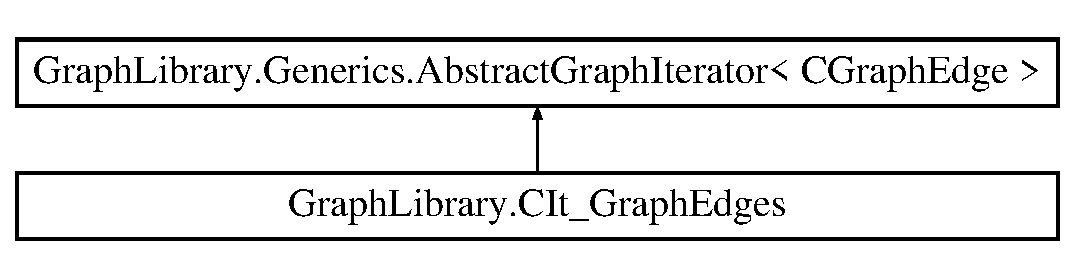
\includegraphics[height=2.000000cm]{class_graph_library_1_1_c_it___graph_edges}
\end{center}
\end{figure}
\subsection*{Public Member Functions}
\begin{DoxyCompactItemize}
\item 
\hyperlink{class_graph_library_1_1_c_it___graph_edges_a10e2198178770159c4652a81eb6a4d1a}{C\+It\+\_\+\+Graph\+Edges} (\hyperlink{class_graph_library_1_1_c_graph}{C\+Graph} graph)
\begin{DoxyCompactList}\small\item\em Constructor \end{DoxyCompactList}\item 
override \hyperlink{class_graph_library_1_1_c_graph_edge}{C\+Graph\+Edge} \hyperlink{class_graph_library_1_1_c_it___graph_edges_a5934153f52d3b0e5bc7de7dbcb3d454d}{Begin} ()
\begin{DoxyCompactList}\small\item\em Points to the first valid item if to null if there is no one \end{DoxyCompactList}\item 
override bool \hyperlink{class_graph_library_1_1_c_it___graph_edges_a64d0c02c22a40db7b62bf7cbf0de02fc}{End} ()
\begin{DoxyCompactList}\small\item\em \hyperlink{class_graph_library_1_1_c_it___graph_edges_a64d0c02c22a40db7b62bf7cbf0de02fc}{End()} function runs after \hyperlink{class_graph_library_1_1_c_it___graph_edges_a5934153f52d3b0e5bc7de7dbcb3d454d}{Begin()} and \hyperlink{class_graph_library_1_1_c_it___graph_edges_ab14c4a444a51dac76ed83211798f05a8}{Next()} functions and before we enter into the loop body. It validates that the iterator points to a proper item \end{DoxyCompactList}\item 
override \hyperlink{class_graph_library_1_1_c_graph_edge}{C\+Graph\+Edge} \hyperlink{class_graph_library_1_1_c_it___graph_edges_ab14c4a444a51dac76ed83211798f05a8}{Next} ()
\begin{DoxyCompactList}\small\item\em Points to the next valid item or to null if there isn\textquotesingle{}t one \end{DoxyCompactList}\end{DoxyCompactItemize}
\subsection*{Additional Inherited Members}


\subsection{Detailed Description}
Iterates over the graph edges 



\subsection{Constructor \& Destructor Documentation}
\hypertarget{class_graph_library_1_1_c_it___graph_edges_a10e2198178770159c4652a81eb6a4d1a}{}\index{Graph\+Library\+::\+C\+It\+\_\+\+Graph\+Edges@{Graph\+Library\+::\+C\+It\+\_\+\+Graph\+Edges}!C\+It\+\_\+\+Graph\+Edges@{C\+It\+\_\+\+Graph\+Edges}}
\index{C\+It\+\_\+\+Graph\+Edges@{C\+It\+\_\+\+Graph\+Edges}!Graph\+Library\+::\+C\+It\+\_\+\+Graph\+Edges@{Graph\+Library\+::\+C\+It\+\_\+\+Graph\+Edges}}
\subsubsection[{C\+It\+\_\+\+Graph\+Edges(\+C\+Graph graph)}]{\setlength{\rightskip}{0pt plus 5cm}Graph\+Library.\+C\+It\+\_\+\+Graph\+Edges.\+C\+It\+\_\+\+Graph\+Edges (
\begin{DoxyParamCaption}
\item[{{\bf C\+Graph}}]{graph}
\end{DoxyParamCaption}
)}\label{class_graph_library_1_1_c_it___graph_edges_a10e2198178770159c4652a81eb6a4d1a}


Constructor 


\begin{DoxyParams}{Parameters}
{\em graph} & \\
\hline
\end{DoxyParams}


\subsection{Member Function Documentation}
\hypertarget{class_graph_library_1_1_c_it___graph_edges_a5934153f52d3b0e5bc7de7dbcb3d454d}{}\index{Graph\+Library\+::\+C\+It\+\_\+\+Graph\+Edges@{Graph\+Library\+::\+C\+It\+\_\+\+Graph\+Edges}!Begin@{Begin}}
\index{Begin@{Begin}!Graph\+Library\+::\+C\+It\+\_\+\+Graph\+Edges@{Graph\+Library\+::\+C\+It\+\_\+\+Graph\+Edges}}
\subsubsection[{Begin()}]{\setlength{\rightskip}{0pt plus 5cm}override {\bf C\+Graph\+Edge} Graph\+Library.\+C\+It\+\_\+\+Graph\+Edges.\+Begin (
\begin{DoxyParamCaption}
{}
\end{DoxyParamCaption}
)\hspace{0.3cm}{\ttfamily [virtual]}}\label{class_graph_library_1_1_c_it___graph_edges_a5934153f52d3b0e5bc7de7dbcb3d454d}


Points to the first valid item if to null if there is no one 

\begin{DoxyReturn}{Returns}

\end{DoxyReturn}


Implements \hyperlink{class_graph_library_1_1_generics_1_1_abstract_graph_iterator_a2c97c7a412c233b8442b7ad403f29779}{Graph\+Library.\+Generics.\+Abstract\+Graph\+Iterator$<$ C\+Graph\+Edge $>$}.

\hypertarget{class_graph_library_1_1_c_it___graph_edges_a64d0c02c22a40db7b62bf7cbf0de02fc}{}\index{Graph\+Library\+::\+C\+It\+\_\+\+Graph\+Edges@{Graph\+Library\+::\+C\+It\+\_\+\+Graph\+Edges}!End@{End}}
\index{End@{End}!Graph\+Library\+::\+C\+It\+\_\+\+Graph\+Edges@{Graph\+Library\+::\+C\+It\+\_\+\+Graph\+Edges}}
\subsubsection[{End()}]{\setlength{\rightskip}{0pt plus 5cm}override bool Graph\+Library.\+C\+It\+\_\+\+Graph\+Edges.\+End (
\begin{DoxyParamCaption}
{}
\end{DoxyParamCaption}
)\hspace{0.3cm}{\ttfamily [virtual]}}\label{class_graph_library_1_1_c_it___graph_edges_a64d0c02c22a40db7b62bf7cbf0de02fc}


\hyperlink{class_graph_library_1_1_c_it___graph_edges_a64d0c02c22a40db7b62bf7cbf0de02fc}{End()} function runs after \hyperlink{class_graph_library_1_1_c_it___graph_edges_a5934153f52d3b0e5bc7de7dbcb3d454d}{Begin()} and \hyperlink{class_graph_library_1_1_c_it___graph_edges_ab14c4a444a51dac76ed83211798f05a8}{Next()} functions and before we enter into the loop body. It validates that the iterator points to a proper item 

\begin{DoxyReturn}{Returns}

\end{DoxyReturn}


Implements \hyperlink{class_graph_library_1_1_generics_1_1_abstract_graph_iterator_aa8cd9f596ec0b6c4c1e9c244ba75df04}{Graph\+Library.\+Generics.\+Abstract\+Graph\+Iterator$<$ C\+Graph\+Edge $>$}.

\hypertarget{class_graph_library_1_1_c_it___graph_edges_ab14c4a444a51dac76ed83211798f05a8}{}\index{Graph\+Library\+::\+C\+It\+\_\+\+Graph\+Edges@{Graph\+Library\+::\+C\+It\+\_\+\+Graph\+Edges}!Next@{Next}}
\index{Next@{Next}!Graph\+Library\+::\+C\+It\+\_\+\+Graph\+Edges@{Graph\+Library\+::\+C\+It\+\_\+\+Graph\+Edges}}
\subsubsection[{Next()}]{\setlength{\rightskip}{0pt plus 5cm}override {\bf C\+Graph\+Edge} Graph\+Library.\+C\+It\+\_\+\+Graph\+Edges.\+Next (
\begin{DoxyParamCaption}
{}
\end{DoxyParamCaption}
)\hspace{0.3cm}{\ttfamily [virtual]}}\label{class_graph_library_1_1_c_it___graph_edges_ab14c4a444a51dac76ed83211798f05a8}


Points to the next valid item or to null if there isn\textquotesingle{}t one 

\begin{DoxyReturn}{Returns}
Returns the current item$<$/returns 
\end{DoxyReturn}


Implements \hyperlink{class_graph_library_1_1_generics_1_1_abstract_graph_iterator_aac8cffd0d579708a94ba056e4f4a00b2}{Graph\+Library.\+Generics.\+Abstract\+Graph\+Iterator$<$ C\+Graph\+Edge $>$}.



The documentation for this class was generated from the following file\+:\begin{DoxyCompactItemize}
\item 
Graph\+Library/Graph\+Iterators.\+cs\end{DoxyCompactItemize}

\hypertarget{class_graph_library_1_1_c_it___graph_leaf_nodes}{}\section{Graph\+Library.\+C\+It\+\_\+\+Graph\+Leaf\+Nodes Class Reference}
\label{class_graph_library_1_1_c_it___graph_leaf_nodes}\index{Graph\+Library.\+C\+It\+\_\+\+Graph\+Leaf\+Nodes@{Graph\+Library.\+C\+It\+\_\+\+Graph\+Leaf\+Nodes}}


Iterates over the graph\textquotesingle{}s nodes not having successors  


Inheritance diagram for Graph\+Library.\+C\+It\+\_\+\+Graph\+Leaf\+Nodes\+:\begin{figure}[H]
\begin{center}
\leavevmode
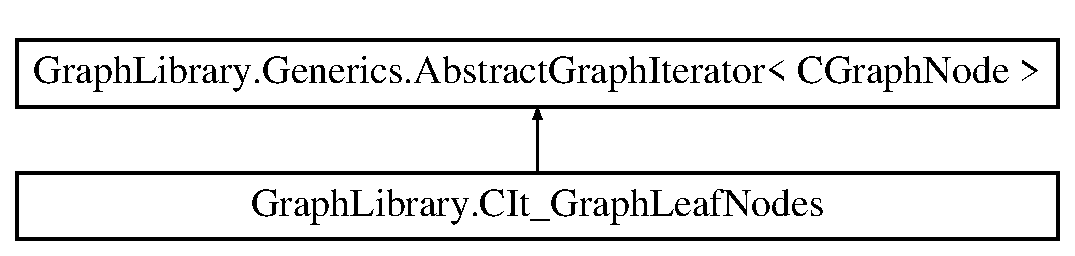
\includegraphics[height=2.000000cm]{class_graph_library_1_1_c_it___graph_leaf_nodes}
\end{center}
\end{figure}
\subsection*{Public Member Functions}
\begin{DoxyCompactItemize}
\item 
\hyperlink{class_graph_library_1_1_c_it___graph_leaf_nodes_a50c1682d64e5c562abdf9ede557daed7}{C\+It\+\_\+\+Graph\+Leaf\+Nodes} (\hyperlink{class_graph_library_1_1_c_graph}{C\+Graph} m\+Graph)
\begin{DoxyCompactList}\small\item\em Initializes a new instance of the \hyperlink{class_graph_library_1_1_c_it___graph_leaf_nodes}{C\+It\+\_\+\+Graph\+Leaf\+Nodes} class. \end{DoxyCompactList}\item 
override \hyperlink{class_graph_library_1_1_c_graph_node}{C\+Graph\+Node} \hyperlink{class_graph_library_1_1_c_it___graph_leaf_nodes_a7f9ce52d3e6c908a50abc991f77b805d}{Begin} ()
\begin{DoxyCompactList}\small\item\em Executes once at the start of the iteration and before the \hyperlink{class_graph_library_1_1_c_it___graph_leaf_nodes_a7a249d8774ff2fef55f20ae8dc1d0fac}{End()} method Initializes the iterator variable ( realized in the subclasses ) and the m\+\_\+current\+Item to point to the first element of the item set. If the set is empty the m\+\_\+current\+Item points to null. After the \hyperlink{class_graph_library_1_1_c_it___graph_leaf_nodes_a7f9ce52d3e6c908a50abc991f77b805d}{Begin()} method the \hyperlink{class_graph_library_1_1_c_it___graph_leaf_nodes_a7a249d8774ff2fef55f20ae8dc1d0fac}{End()} method executes before going into the loop body. Thus the loop terminates if the item set is empty before ever running the loop body The transition logic for finding the first item in the items set is implemented in the subclasses \end{DoxyCompactList}\item 
override bool \hyperlink{class_graph_library_1_1_c_it___graph_leaf_nodes_a7a249d8774ff2fef55f20ae8dc1d0fac}{End} ()
\begin{DoxyCompactList}\small\item\em Executes after the \hyperlink{class_graph_library_1_1_c_it___graph_leaf_nodes_a7f9ce52d3e6c908a50abc991f77b805d}{Begin()} or \hyperlink{class_graph_library_1_1_c_it___graph_leaf_nodes_aa6f30fbeebae338fa9d77455027679f0}{Next()} methods and before the Loop Body Returns true if the m\+\_\+current\+Item is null. This case arises in the following scenarios\+: 1) The item set is empty thus, after the \hyperlink{class_graph_library_1_1_c_it___graph_leaf_nodes_a7f9ce52d3e6c908a50abc991f77b805d}{Begin()} method call the \hyperlink{class_graph_library_1_1_c_it___graph_leaf_nodes_a7a249d8774ff2fef55f20ae8dc1d0fac}{End()} identifies that m\+\_\+current\+Item points to null 2) The item set is not empty and the iterator went outside the boundaries of the item set after the call to \hyperlink{class_graph_library_1_1_c_it___graph_leaf_nodes_aa6f30fbeebae338fa9d77455027679f0}{Next()} method (\hyperlink{class_graph_library_1_1_c_it___graph_leaf_nodes_aa6f30fbeebae338fa9d77455027679f0}{Next()} method set m\+\_\+current\+Item to null) \end{DoxyCompactList}\item 
override \hyperlink{class_graph_library_1_1_c_graph_node}{C\+Graph\+Node} \hyperlink{class_graph_library_1_1_c_it___graph_leaf_nodes_aa6f30fbeebae338fa9d77455027679f0}{Next} ()
\begin{DoxyCompactList}\small\item\em Executes after the execution of the loop body and before the \hyperlink{class_graph_library_1_1_c_it___graph_leaf_nodes_a7a249d8774ff2fef55f20ae8dc1d0fac}{End()} method Increases the iteration variable and set the m\+\_\+current\+Item to point to the current item of the item set. In case where the end of the item set is reached the m\+\_\+current\+Item points to null which is identified by the \hyperlink{class_graph_library_1_1_c_it___graph_leaf_nodes_a7a249d8774ff2fef55f20ae8dc1d0fac}{End()} methods that is executed next. The transition logic from item to item is implemented from the subclasses. \end{DoxyCompactList}\end{DoxyCompactItemize}
\subsection*{Additional Inherited Members}


\subsection{Detailed Description}
Iterates over the graph\textquotesingle{}s nodes not having successors 



\subsection{Constructor \& Destructor Documentation}
\hypertarget{class_graph_library_1_1_c_it___graph_leaf_nodes_a50c1682d64e5c562abdf9ede557daed7}{}\index{Graph\+Library\+::\+C\+It\+\_\+\+Graph\+Leaf\+Nodes@{Graph\+Library\+::\+C\+It\+\_\+\+Graph\+Leaf\+Nodes}!C\+It\+\_\+\+Graph\+Leaf\+Nodes@{C\+It\+\_\+\+Graph\+Leaf\+Nodes}}
\index{C\+It\+\_\+\+Graph\+Leaf\+Nodes@{C\+It\+\_\+\+Graph\+Leaf\+Nodes}!Graph\+Library\+::\+C\+It\+\_\+\+Graph\+Leaf\+Nodes@{Graph\+Library\+::\+C\+It\+\_\+\+Graph\+Leaf\+Nodes}}
\subsubsection[{C\+It\+\_\+\+Graph\+Leaf\+Nodes(\+C\+Graph m\+Graph)}]{\setlength{\rightskip}{0pt plus 5cm}Graph\+Library.\+C\+It\+\_\+\+Graph\+Leaf\+Nodes.\+C\+It\+\_\+\+Graph\+Leaf\+Nodes (
\begin{DoxyParamCaption}
\item[{{\bf C\+Graph}}]{m\+Graph}
\end{DoxyParamCaption}
)}\label{class_graph_library_1_1_c_it___graph_leaf_nodes_a50c1682d64e5c562abdf9ede557daed7}


Initializes a new instance of the \hyperlink{class_graph_library_1_1_c_it___graph_leaf_nodes}{C\+It\+\_\+\+Graph\+Leaf\+Nodes} class. 


\begin{DoxyParams}{Parameters}
{\em m\+Graph} & The m graph.\\
\hline
\end{DoxyParams}


\subsection{Member Function Documentation}
\hypertarget{class_graph_library_1_1_c_it___graph_leaf_nodes_a7f9ce52d3e6c908a50abc991f77b805d}{}\index{Graph\+Library\+::\+C\+It\+\_\+\+Graph\+Leaf\+Nodes@{Graph\+Library\+::\+C\+It\+\_\+\+Graph\+Leaf\+Nodes}!Begin@{Begin}}
\index{Begin@{Begin}!Graph\+Library\+::\+C\+It\+\_\+\+Graph\+Leaf\+Nodes@{Graph\+Library\+::\+C\+It\+\_\+\+Graph\+Leaf\+Nodes}}
\subsubsection[{Begin()}]{\setlength{\rightskip}{0pt plus 5cm}override {\bf C\+Graph\+Node} Graph\+Library.\+C\+It\+\_\+\+Graph\+Leaf\+Nodes.\+Begin (
\begin{DoxyParamCaption}
{}
\end{DoxyParamCaption}
)\hspace{0.3cm}{\ttfamily [virtual]}}\label{class_graph_library_1_1_c_it___graph_leaf_nodes_a7f9ce52d3e6c908a50abc991f77b805d}


Executes once at the start of the iteration and before the \hyperlink{class_graph_library_1_1_c_it___graph_leaf_nodes_a7a249d8774ff2fef55f20ae8dc1d0fac}{End()} method Initializes the iterator variable ( realized in the subclasses ) and the m\+\_\+current\+Item to point to the first element of the item set. If the set is empty the m\+\_\+current\+Item points to null. After the \hyperlink{class_graph_library_1_1_c_it___graph_leaf_nodes_a7f9ce52d3e6c908a50abc991f77b805d}{Begin()} method the \hyperlink{class_graph_library_1_1_c_it___graph_leaf_nodes_a7a249d8774ff2fef55f20ae8dc1d0fac}{End()} method executes before going into the loop body. Thus the loop terminates if the item set is empty before ever running the loop body The transition logic for finding the first item in the items set is implemented in the subclasses 

\begin{DoxyReturn}{Returns}

\end{DoxyReturn}


Implements \hyperlink{class_graph_library_1_1_generics_1_1_abstract_graph_iterator_a2c97c7a412c233b8442b7ad403f29779}{Graph\+Library.\+Generics.\+Abstract\+Graph\+Iterator$<$ C\+Graph\+Node $>$}.

\hypertarget{class_graph_library_1_1_c_it___graph_leaf_nodes_a7a249d8774ff2fef55f20ae8dc1d0fac}{}\index{Graph\+Library\+::\+C\+It\+\_\+\+Graph\+Leaf\+Nodes@{Graph\+Library\+::\+C\+It\+\_\+\+Graph\+Leaf\+Nodes}!End@{End}}
\index{End@{End}!Graph\+Library\+::\+C\+It\+\_\+\+Graph\+Leaf\+Nodes@{Graph\+Library\+::\+C\+It\+\_\+\+Graph\+Leaf\+Nodes}}
\subsubsection[{End()}]{\setlength{\rightskip}{0pt plus 5cm}override bool Graph\+Library.\+C\+It\+\_\+\+Graph\+Leaf\+Nodes.\+End (
\begin{DoxyParamCaption}
{}
\end{DoxyParamCaption}
)\hspace{0.3cm}{\ttfamily [virtual]}}\label{class_graph_library_1_1_c_it___graph_leaf_nodes_a7a249d8774ff2fef55f20ae8dc1d0fac}


Executes after the \hyperlink{class_graph_library_1_1_c_it___graph_leaf_nodes_a7f9ce52d3e6c908a50abc991f77b805d}{Begin()} or \hyperlink{class_graph_library_1_1_c_it___graph_leaf_nodes_aa6f30fbeebae338fa9d77455027679f0}{Next()} methods and before the Loop Body Returns true if the m\+\_\+current\+Item is null. This case arises in the following scenarios\+: 1) The item set is empty thus, after the \hyperlink{class_graph_library_1_1_c_it___graph_leaf_nodes_a7f9ce52d3e6c908a50abc991f77b805d}{Begin()} method call the \hyperlink{class_graph_library_1_1_c_it___graph_leaf_nodes_a7a249d8774ff2fef55f20ae8dc1d0fac}{End()} identifies that m\+\_\+current\+Item points to null 2) The item set is not empty and the iterator went outside the boundaries of the item set after the call to \hyperlink{class_graph_library_1_1_c_it___graph_leaf_nodes_aa6f30fbeebae338fa9d77455027679f0}{Next()} method (\hyperlink{class_graph_library_1_1_c_it___graph_leaf_nodes_aa6f30fbeebae338fa9d77455027679f0}{Next()} method set m\+\_\+current\+Item to null) 

\begin{DoxyReturn}{Returns}

\end{DoxyReturn}


Implements \hyperlink{class_graph_library_1_1_generics_1_1_abstract_graph_iterator_aa8cd9f596ec0b6c4c1e9c244ba75df04}{Graph\+Library.\+Generics.\+Abstract\+Graph\+Iterator$<$ C\+Graph\+Node $>$}.

\hypertarget{class_graph_library_1_1_c_it___graph_leaf_nodes_aa6f30fbeebae338fa9d77455027679f0}{}\index{Graph\+Library\+::\+C\+It\+\_\+\+Graph\+Leaf\+Nodes@{Graph\+Library\+::\+C\+It\+\_\+\+Graph\+Leaf\+Nodes}!Next@{Next}}
\index{Next@{Next}!Graph\+Library\+::\+C\+It\+\_\+\+Graph\+Leaf\+Nodes@{Graph\+Library\+::\+C\+It\+\_\+\+Graph\+Leaf\+Nodes}}
\subsubsection[{Next()}]{\setlength{\rightskip}{0pt plus 5cm}override {\bf C\+Graph\+Node} Graph\+Library.\+C\+It\+\_\+\+Graph\+Leaf\+Nodes.\+Next (
\begin{DoxyParamCaption}
{}
\end{DoxyParamCaption}
)\hspace{0.3cm}{\ttfamily [virtual]}}\label{class_graph_library_1_1_c_it___graph_leaf_nodes_aa6f30fbeebae338fa9d77455027679f0}


Executes after the execution of the loop body and before the \hyperlink{class_graph_library_1_1_c_it___graph_leaf_nodes_a7a249d8774ff2fef55f20ae8dc1d0fac}{End()} method Increases the iteration variable and set the m\+\_\+current\+Item to point to the current item of the item set. In case where the end of the item set is reached the m\+\_\+current\+Item points to null which is identified by the \hyperlink{class_graph_library_1_1_c_it___graph_leaf_nodes_a7a249d8774ff2fef55f20ae8dc1d0fac}{End()} methods that is executed next. The transition logic from item to item is implemented from the subclasses. 

\begin{DoxyReturn}{Returns}

\end{DoxyReturn}


Implements \hyperlink{class_graph_library_1_1_generics_1_1_abstract_graph_iterator_aac8cffd0d579708a94ba056e4f4a00b2}{Graph\+Library.\+Generics.\+Abstract\+Graph\+Iterator$<$ C\+Graph\+Node $>$}.



The documentation for this class was generated from the following file\+:\begin{DoxyCompactItemize}
\item 
Graph\+Library/Graph\+Iterators.\+cs\end{DoxyCompactItemize}

\hypertarget{class_graph_library_1_1_c_it___graph_nodes}{}\section{Graph\+Library.\+C\+It\+\_\+\+Graph\+Nodes Class Reference}
\label{class_graph_library_1_1_c_it___graph_nodes}\index{Graph\+Library.\+C\+It\+\_\+\+Graph\+Nodes@{Graph\+Library.\+C\+It\+\_\+\+Graph\+Nodes}}


Iterates over the graph nodes  


Inheritance diagram for Graph\+Library.\+C\+It\+\_\+\+Graph\+Nodes\+:\begin{figure}[H]
\begin{center}
\leavevmode
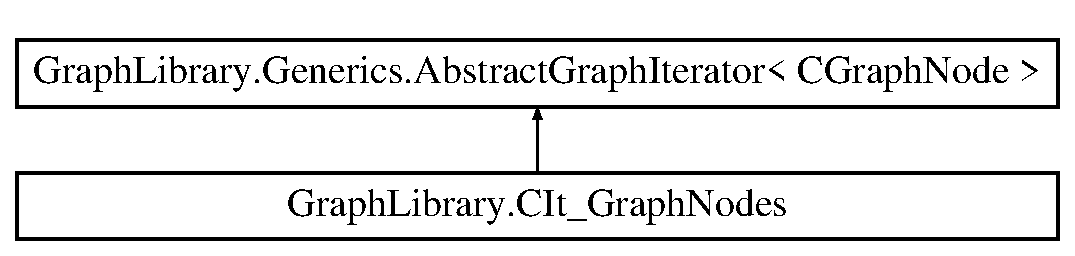
\includegraphics[height=2.000000cm]{class_graph_library_1_1_c_it___graph_nodes}
\end{center}
\end{figure}
\subsection*{Public Member Functions}
\begin{DoxyCompactItemize}
\item 
\hyperlink{class_graph_library_1_1_c_it___graph_nodes_aa4e91b5296c753d11ec54a7efe92efed}{C\+It\+\_\+\+Graph\+Nodes} (\hyperlink{class_graph_library_1_1_c_graph}{C\+Graph} graph)
\begin{DoxyCompactList}\small\item\em Constructor \end{DoxyCompactList}\item 
override \hyperlink{class_graph_library_1_1_c_graph_node}{C\+Graph\+Node} \hyperlink{class_graph_library_1_1_c_it___graph_nodes_a19eafdc8ea743803dddcc5a9a73adbf6}{Begin} ()
\begin{DoxyCompactList}\small\item\em Points to the first valid item if to null if there is no one \end{DoxyCompactList}\item 
override bool \hyperlink{class_graph_library_1_1_c_it___graph_nodes_abb9dc813b7bf7ff0aa0a22ef83ba3478}{End} ()
\begin{DoxyCompactList}\small\item\em \hyperlink{class_graph_library_1_1_c_it___graph_nodes_abb9dc813b7bf7ff0aa0a22ef83ba3478}{End()} function runs after \hyperlink{class_graph_library_1_1_c_it___graph_nodes_a19eafdc8ea743803dddcc5a9a73adbf6}{Begin()} and \hyperlink{class_graph_library_1_1_c_it___graph_nodes_a669edb9e8d59c4dcdbb70fe15e89104a}{Next()} functions and before we enter into the loop body. It validates that the iterator points to a proper item \end{DoxyCompactList}\item 
override \hyperlink{class_graph_library_1_1_c_graph_node}{C\+Graph\+Node} \hyperlink{class_graph_library_1_1_c_it___graph_nodes_a669edb9e8d59c4dcdbb70fe15e89104a}{Next} ()
\begin{DoxyCompactList}\small\item\em Points to the next valid item or to null if there isn\textquotesingle{}t one \end{DoxyCompactList}\end{DoxyCompactItemize}
\subsection*{Additional Inherited Members}


\subsection{Detailed Description}
Iterates over the graph nodes 



\subsection{Constructor \& Destructor Documentation}
\hypertarget{class_graph_library_1_1_c_it___graph_nodes_aa4e91b5296c753d11ec54a7efe92efed}{}\index{Graph\+Library\+::\+C\+It\+\_\+\+Graph\+Nodes@{Graph\+Library\+::\+C\+It\+\_\+\+Graph\+Nodes}!C\+It\+\_\+\+Graph\+Nodes@{C\+It\+\_\+\+Graph\+Nodes}}
\index{C\+It\+\_\+\+Graph\+Nodes@{C\+It\+\_\+\+Graph\+Nodes}!Graph\+Library\+::\+C\+It\+\_\+\+Graph\+Nodes@{Graph\+Library\+::\+C\+It\+\_\+\+Graph\+Nodes}}
\subsubsection[{C\+It\+\_\+\+Graph\+Nodes(\+C\+Graph graph)}]{\setlength{\rightskip}{0pt plus 5cm}Graph\+Library.\+C\+It\+\_\+\+Graph\+Nodes.\+C\+It\+\_\+\+Graph\+Nodes (
\begin{DoxyParamCaption}
\item[{{\bf C\+Graph}}]{graph}
\end{DoxyParamCaption}
)}\label{class_graph_library_1_1_c_it___graph_nodes_aa4e91b5296c753d11ec54a7efe92efed}


Constructor 


\begin{DoxyParams}{Parameters}
{\em graph} & \\
\hline
\end{DoxyParams}


\subsection{Member Function Documentation}
\hypertarget{class_graph_library_1_1_c_it___graph_nodes_a19eafdc8ea743803dddcc5a9a73adbf6}{}\index{Graph\+Library\+::\+C\+It\+\_\+\+Graph\+Nodes@{Graph\+Library\+::\+C\+It\+\_\+\+Graph\+Nodes}!Begin@{Begin}}
\index{Begin@{Begin}!Graph\+Library\+::\+C\+It\+\_\+\+Graph\+Nodes@{Graph\+Library\+::\+C\+It\+\_\+\+Graph\+Nodes}}
\subsubsection[{Begin()}]{\setlength{\rightskip}{0pt plus 5cm}override {\bf C\+Graph\+Node} Graph\+Library.\+C\+It\+\_\+\+Graph\+Nodes.\+Begin (
\begin{DoxyParamCaption}
{}
\end{DoxyParamCaption}
)\hspace{0.3cm}{\ttfamily [virtual]}}\label{class_graph_library_1_1_c_it___graph_nodes_a19eafdc8ea743803dddcc5a9a73adbf6}


Points to the first valid item if to null if there is no one 

\begin{DoxyReturn}{Returns}

\end{DoxyReturn}


Implements \hyperlink{class_graph_library_1_1_generics_1_1_abstract_graph_iterator_a2c97c7a412c233b8442b7ad403f29779}{Graph\+Library.\+Generics.\+Abstract\+Graph\+Iterator$<$ C\+Graph\+Node $>$}.

\hypertarget{class_graph_library_1_1_c_it___graph_nodes_abb9dc813b7bf7ff0aa0a22ef83ba3478}{}\index{Graph\+Library\+::\+C\+It\+\_\+\+Graph\+Nodes@{Graph\+Library\+::\+C\+It\+\_\+\+Graph\+Nodes}!End@{End}}
\index{End@{End}!Graph\+Library\+::\+C\+It\+\_\+\+Graph\+Nodes@{Graph\+Library\+::\+C\+It\+\_\+\+Graph\+Nodes}}
\subsubsection[{End()}]{\setlength{\rightskip}{0pt plus 5cm}override bool Graph\+Library.\+C\+It\+\_\+\+Graph\+Nodes.\+End (
\begin{DoxyParamCaption}
{}
\end{DoxyParamCaption}
)\hspace{0.3cm}{\ttfamily [virtual]}}\label{class_graph_library_1_1_c_it___graph_nodes_abb9dc813b7bf7ff0aa0a22ef83ba3478}


\hyperlink{class_graph_library_1_1_c_it___graph_nodes_abb9dc813b7bf7ff0aa0a22ef83ba3478}{End()} function runs after \hyperlink{class_graph_library_1_1_c_it___graph_nodes_a19eafdc8ea743803dddcc5a9a73adbf6}{Begin()} and \hyperlink{class_graph_library_1_1_c_it___graph_nodes_a669edb9e8d59c4dcdbb70fe15e89104a}{Next()} functions and before we enter into the loop body. It validates that the iterator points to a proper item 

\begin{DoxyReturn}{Returns}

\end{DoxyReturn}


Implements \hyperlink{class_graph_library_1_1_generics_1_1_abstract_graph_iterator_aa8cd9f596ec0b6c4c1e9c244ba75df04}{Graph\+Library.\+Generics.\+Abstract\+Graph\+Iterator$<$ C\+Graph\+Node $>$}.

\hypertarget{class_graph_library_1_1_c_it___graph_nodes_a669edb9e8d59c4dcdbb70fe15e89104a}{}\index{Graph\+Library\+::\+C\+It\+\_\+\+Graph\+Nodes@{Graph\+Library\+::\+C\+It\+\_\+\+Graph\+Nodes}!Next@{Next}}
\index{Next@{Next}!Graph\+Library\+::\+C\+It\+\_\+\+Graph\+Nodes@{Graph\+Library\+::\+C\+It\+\_\+\+Graph\+Nodes}}
\subsubsection[{Next()}]{\setlength{\rightskip}{0pt plus 5cm}override {\bf C\+Graph\+Node} Graph\+Library.\+C\+It\+\_\+\+Graph\+Nodes.\+Next (
\begin{DoxyParamCaption}
{}
\end{DoxyParamCaption}
)\hspace{0.3cm}{\ttfamily [virtual]}}\label{class_graph_library_1_1_c_it___graph_nodes_a669edb9e8d59c4dcdbb70fe15e89104a}


Points to the next valid item or to null if there isn\textquotesingle{}t one 

\begin{DoxyReturn}{Returns}
Returns the current item$<$/returns 
\end{DoxyReturn}


Implements \hyperlink{class_graph_library_1_1_generics_1_1_abstract_graph_iterator_aac8cffd0d579708a94ba056e4f4a00b2}{Graph\+Library.\+Generics.\+Abstract\+Graph\+Iterator$<$ C\+Graph\+Node $>$}.



The documentation for this class was generated from the following file\+:\begin{DoxyCompactItemize}
\item 
Graph\+Library/Graph\+Iterators.\+cs\end{DoxyCompactItemize}

\hypertarget{class_graph_library_1_1_c_it___graph_root_nodes}{}\section{Graph\+Library.\+C\+It\+\_\+\+Graph\+Root\+Nodes Class Reference}
\label{class_graph_library_1_1_c_it___graph_root_nodes}\index{Graph\+Library.\+C\+It\+\_\+\+Graph\+Root\+Nodes@{Graph\+Library.\+C\+It\+\_\+\+Graph\+Root\+Nodes}}


Iterates over the graph\textquotesingle{}s nodes not having predecessors  


Inheritance diagram for Graph\+Library.\+C\+It\+\_\+\+Graph\+Root\+Nodes\+:\begin{figure}[H]
\begin{center}
\leavevmode
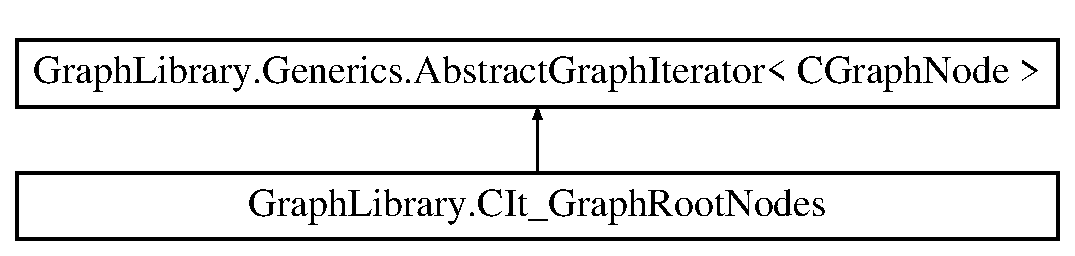
\includegraphics[height=2.000000cm]{class_graph_library_1_1_c_it___graph_root_nodes}
\end{center}
\end{figure}
\subsection*{Public Member Functions}
\begin{DoxyCompactItemize}
\item 
\hypertarget{class_graph_library_1_1_c_it___graph_root_nodes_a67dfd1fbc6fd3de58b1084703f29590f}{}{\bfseries C\+It\+\_\+\+Graph\+Root\+Nodes} (\hyperlink{class_graph_library_1_1_c_graph}{C\+Graph} m\+Graph)\label{class_graph_library_1_1_c_it___graph_root_nodes_a67dfd1fbc6fd3de58b1084703f29590f}

\item 
override \hyperlink{class_graph_library_1_1_c_graph_node}{C\+Graph\+Node} \hyperlink{class_graph_library_1_1_c_it___graph_root_nodes_a582dd6795006075f6f81fef42d1de1ba}{Begin} ()
\begin{DoxyCompactList}\small\item\em Executes once at the start of the iteration and before the \hyperlink{class_graph_library_1_1_c_it___graph_root_nodes_a1173c503776973a5e4f6f51492f21fe5}{End()} method Initializes the iterator variable ( realized in the subclasses ) and the m\+\_\+current\+Item to point to the first element of the item set. If the set is empty the m\+\_\+current\+Item points to null. After the \hyperlink{class_graph_library_1_1_c_it___graph_root_nodes_a582dd6795006075f6f81fef42d1de1ba}{Begin()} method the \hyperlink{class_graph_library_1_1_c_it___graph_root_nodes_a1173c503776973a5e4f6f51492f21fe5}{End()} method executes before going into the loop body. Thus the loop terminates if the item set is empty before ever running the loop body The transition logic for finding the first item in the items set is implemented in the subclasses \end{DoxyCompactList}\item 
override bool \hyperlink{class_graph_library_1_1_c_it___graph_root_nodes_a1173c503776973a5e4f6f51492f21fe5}{End} ()
\begin{DoxyCompactList}\small\item\em Executes after the \hyperlink{class_graph_library_1_1_c_it___graph_root_nodes_a582dd6795006075f6f81fef42d1de1ba}{Begin()} or \hyperlink{class_graph_library_1_1_c_it___graph_root_nodes_a4606ecd1ef26c19634171ccd81e18816}{Next()} methods and before the Loop Body Returns true if the m\+\_\+current\+Item is null. This case arises in the following scenarios\+: 1) The item set is empty thus, after the \hyperlink{class_graph_library_1_1_c_it___graph_root_nodes_a582dd6795006075f6f81fef42d1de1ba}{Begin()} method call the \hyperlink{class_graph_library_1_1_c_it___graph_root_nodes_a1173c503776973a5e4f6f51492f21fe5}{End()} identifies that m\+\_\+current\+Item points to null 2) The item set is not empty and the iterator went outside the boundaries of the item set after the call to \hyperlink{class_graph_library_1_1_c_it___graph_root_nodes_a4606ecd1ef26c19634171ccd81e18816}{Next()} method (\hyperlink{class_graph_library_1_1_c_it___graph_root_nodes_a4606ecd1ef26c19634171ccd81e18816}{Next()} method set m\+\_\+current\+Item to null) \end{DoxyCompactList}\item 
override \hyperlink{class_graph_library_1_1_c_graph_node}{C\+Graph\+Node} \hyperlink{class_graph_library_1_1_c_it___graph_root_nodes_a4606ecd1ef26c19634171ccd81e18816}{Next} ()
\begin{DoxyCompactList}\small\item\em Executes after the execution of the loop body and before the \hyperlink{class_graph_library_1_1_c_it___graph_root_nodes_a1173c503776973a5e4f6f51492f21fe5}{End()} method Increases the iteration variable and set the m\+\_\+current\+Item to point to the current item of the item set. In case where the end of the item set is reached the m\+\_\+current\+Item points to null which is identified by the \hyperlink{class_graph_library_1_1_c_it___graph_root_nodes_a1173c503776973a5e4f6f51492f21fe5}{End()} methods that is executed next. The transition logic from item to item is implemented from the subclasses. \end{DoxyCompactList}\end{DoxyCompactItemize}
\subsection*{Additional Inherited Members}


\subsection{Detailed Description}
Iterates over the graph\textquotesingle{}s nodes not having predecessors 



\subsection{Member Function Documentation}
\hypertarget{class_graph_library_1_1_c_it___graph_root_nodes_a582dd6795006075f6f81fef42d1de1ba}{}\index{Graph\+Library\+::\+C\+It\+\_\+\+Graph\+Root\+Nodes@{Graph\+Library\+::\+C\+It\+\_\+\+Graph\+Root\+Nodes}!Begin@{Begin}}
\index{Begin@{Begin}!Graph\+Library\+::\+C\+It\+\_\+\+Graph\+Root\+Nodes@{Graph\+Library\+::\+C\+It\+\_\+\+Graph\+Root\+Nodes}}
\subsubsection[{Begin()}]{\setlength{\rightskip}{0pt plus 5cm}override {\bf C\+Graph\+Node} Graph\+Library.\+C\+It\+\_\+\+Graph\+Root\+Nodes.\+Begin (
\begin{DoxyParamCaption}
{}
\end{DoxyParamCaption}
)\hspace{0.3cm}{\ttfamily [virtual]}}\label{class_graph_library_1_1_c_it___graph_root_nodes_a582dd6795006075f6f81fef42d1de1ba}


Executes once at the start of the iteration and before the \hyperlink{class_graph_library_1_1_c_it___graph_root_nodes_a1173c503776973a5e4f6f51492f21fe5}{End()} method Initializes the iterator variable ( realized in the subclasses ) and the m\+\_\+current\+Item to point to the first element of the item set. If the set is empty the m\+\_\+current\+Item points to null. After the \hyperlink{class_graph_library_1_1_c_it___graph_root_nodes_a582dd6795006075f6f81fef42d1de1ba}{Begin()} method the \hyperlink{class_graph_library_1_1_c_it___graph_root_nodes_a1173c503776973a5e4f6f51492f21fe5}{End()} method executes before going into the loop body. Thus the loop terminates if the item set is empty before ever running the loop body The transition logic for finding the first item in the items set is implemented in the subclasses 

\begin{DoxyReturn}{Returns}

\end{DoxyReturn}


Implements \hyperlink{class_graph_library_1_1_generics_1_1_abstract_graph_iterator_a2c97c7a412c233b8442b7ad403f29779}{Graph\+Library.\+Generics.\+Abstract\+Graph\+Iterator$<$ C\+Graph\+Node $>$}.

\hypertarget{class_graph_library_1_1_c_it___graph_root_nodes_a1173c503776973a5e4f6f51492f21fe5}{}\index{Graph\+Library\+::\+C\+It\+\_\+\+Graph\+Root\+Nodes@{Graph\+Library\+::\+C\+It\+\_\+\+Graph\+Root\+Nodes}!End@{End}}
\index{End@{End}!Graph\+Library\+::\+C\+It\+\_\+\+Graph\+Root\+Nodes@{Graph\+Library\+::\+C\+It\+\_\+\+Graph\+Root\+Nodes}}
\subsubsection[{End()}]{\setlength{\rightskip}{0pt plus 5cm}override bool Graph\+Library.\+C\+It\+\_\+\+Graph\+Root\+Nodes.\+End (
\begin{DoxyParamCaption}
{}
\end{DoxyParamCaption}
)\hspace{0.3cm}{\ttfamily [virtual]}}\label{class_graph_library_1_1_c_it___graph_root_nodes_a1173c503776973a5e4f6f51492f21fe5}


Executes after the \hyperlink{class_graph_library_1_1_c_it___graph_root_nodes_a582dd6795006075f6f81fef42d1de1ba}{Begin()} or \hyperlink{class_graph_library_1_1_c_it___graph_root_nodes_a4606ecd1ef26c19634171ccd81e18816}{Next()} methods and before the Loop Body Returns true if the m\+\_\+current\+Item is null. This case arises in the following scenarios\+: 1) The item set is empty thus, after the \hyperlink{class_graph_library_1_1_c_it___graph_root_nodes_a582dd6795006075f6f81fef42d1de1ba}{Begin()} method call the \hyperlink{class_graph_library_1_1_c_it___graph_root_nodes_a1173c503776973a5e4f6f51492f21fe5}{End()} identifies that m\+\_\+current\+Item points to null 2) The item set is not empty and the iterator went outside the boundaries of the item set after the call to \hyperlink{class_graph_library_1_1_c_it___graph_root_nodes_a4606ecd1ef26c19634171ccd81e18816}{Next()} method (\hyperlink{class_graph_library_1_1_c_it___graph_root_nodes_a4606ecd1ef26c19634171ccd81e18816}{Next()} method set m\+\_\+current\+Item to null) 

\begin{DoxyReturn}{Returns}

\end{DoxyReturn}


Implements \hyperlink{class_graph_library_1_1_generics_1_1_abstract_graph_iterator_aa8cd9f596ec0b6c4c1e9c244ba75df04}{Graph\+Library.\+Generics.\+Abstract\+Graph\+Iterator$<$ C\+Graph\+Node $>$}.

\hypertarget{class_graph_library_1_1_c_it___graph_root_nodes_a4606ecd1ef26c19634171ccd81e18816}{}\index{Graph\+Library\+::\+C\+It\+\_\+\+Graph\+Root\+Nodes@{Graph\+Library\+::\+C\+It\+\_\+\+Graph\+Root\+Nodes}!Next@{Next}}
\index{Next@{Next}!Graph\+Library\+::\+C\+It\+\_\+\+Graph\+Root\+Nodes@{Graph\+Library\+::\+C\+It\+\_\+\+Graph\+Root\+Nodes}}
\subsubsection[{Next()}]{\setlength{\rightskip}{0pt plus 5cm}override {\bf C\+Graph\+Node} Graph\+Library.\+C\+It\+\_\+\+Graph\+Root\+Nodes.\+Next (
\begin{DoxyParamCaption}
{}
\end{DoxyParamCaption}
)\hspace{0.3cm}{\ttfamily [virtual]}}\label{class_graph_library_1_1_c_it___graph_root_nodes_a4606ecd1ef26c19634171ccd81e18816}


Executes after the execution of the loop body and before the \hyperlink{class_graph_library_1_1_c_it___graph_root_nodes_a1173c503776973a5e4f6f51492f21fe5}{End()} method Increases the iteration variable and set the m\+\_\+current\+Item to point to the current item of the item set. In case where the end of the item set is reached the m\+\_\+current\+Item points to null which is identified by the \hyperlink{class_graph_library_1_1_c_it___graph_root_nodes_a1173c503776973a5e4f6f51492f21fe5}{End()} methods that is executed next. The transition logic from item to item is implemented from the subclasses. 

\begin{DoxyReturn}{Returns}

\end{DoxyReturn}


Implements \hyperlink{class_graph_library_1_1_generics_1_1_abstract_graph_iterator_aac8cffd0d579708a94ba056e4f4a00b2}{Graph\+Library.\+Generics.\+Abstract\+Graph\+Iterator$<$ C\+Graph\+Node $>$}.



The documentation for this class was generated from the following file\+:\begin{DoxyCompactItemize}
\item 
Graph\+Library/Graph\+Iterators.\+cs\end{DoxyCompactItemize}

\hypertarget{class_graph_library_1_1_c_it___predecessors}{}\section{Graph\+Library.\+C\+It\+\_\+\+Predecessors Class Reference}
\label{class_graph_library_1_1_c_it___predecessors}\index{Graph\+Library.\+C\+It\+\_\+\+Predecessors@{Graph\+Library.\+C\+It\+\_\+\+Predecessors}}


Iterates over the predecessor nodes of a node  


Inheritance diagram for Graph\+Library.\+C\+It\+\_\+\+Predecessors\+:\begin{figure}[H]
\begin{center}
\leavevmode
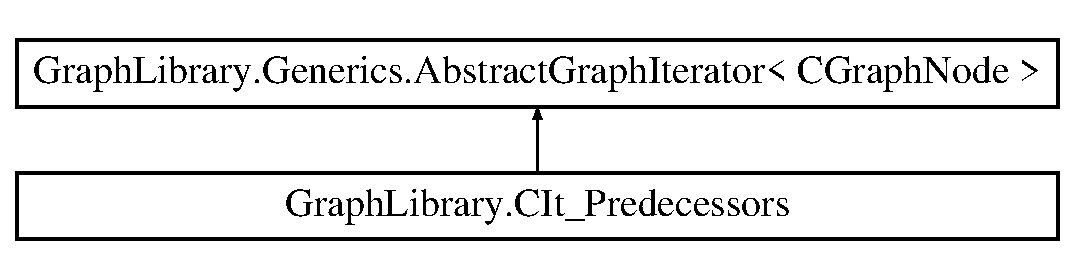
\includegraphics[height=2.000000cm]{class_graph_library_1_1_c_it___predecessors}
\end{center}
\end{figure}
\subsection*{Public Member Functions}
\begin{DoxyCompactItemize}
\item 
\hyperlink{class_graph_library_1_1_c_it___predecessors_ab9fa002e3d6b597d7712faab5613cbe3}{C\+It\+\_\+\+Predecessors} (\hyperlink{class_graph_library_1_1_c_graph_node}{C\+Graph\+Node} node)
\begin{DoxyCompactList}\small\item\em Constructor. Takes the node to which it refers \end{DoxyCompactList}\item 
override \hyperlink{class_graph_library_1_1_c_graph_node}{C\+Graph\+Node} \hyperlink{class_graph_library_1_1_c_it___predecessors_aa71033bdb63459cb6bac0c01db43bf6d}{Begin} ()
\begin{DoxyCompactList}\small\item\em Points to the first valid item if to null if there is no one \end{DoxyCompactList}\item 
override bool \hyperlink{class_graph_library_1_1_c_it___predecessors_a01294d5cb0b22ddc2e8c39edc5d2cc01}{End} ()
\begin{DoxyCompactList}\small\item\em \hyperlink{class_graph_library_1_1_c_it___predecessors_a01294d5cb0b22ddc2e8c39edc5d2cc01}{End()} function runs after \hyperlink{class_graph_library_1_1_c_it___predecessors_aa71033bdb63459cb6bac0c01db43bf6d}{Begin()} and \hyperlink{class_graph_library_1_1_c_it___predecessors_a560fdfb437097d41b4c7dd15905eae99}{Next()} functions and before we enter into the loop body. It validates that the iterator points to a proper item \end{DoxyCompactList}\item 
override \hyperlink{class_graph_library_1_1_c_graph_node}{C\+Graph\+Node} \hyperlink{class_graph_library_1_1_c_it___predecessors_a560fdfb437097d41b4c7dd15905eae99}{Next} ()
\begin{DoxyCompactList}\small\item\em Points to the next valid item or to null if there isn\textquotesingle{}t one \end{DoxyCompactList}\end{DoxyCompactItemize}
\subsection*{Additional Inherited Members}


\subsection{Detailed Description}
Iterates over the predecessor nodes of a node 



\subsection{Constructor \& Destructor Documentation}
\hypertarget{class_graph_library_1_1_c_it___predecessors_ab9fa002e3d6b597d7712faab5613cbe3}{}\index{Graph\+Library\+::\+C\+It\+\_\+\+Predecessors@{Graph\+Library\+::\+C\+It\+\_\+\+Predecessors}!C\+It\+\_\+\+Predecessors@{C\+It\+\_\+\+Predecessors}}
\index{C\+It\+\_\+\+Predecessors@{C\+It\+\_\+\+Predecessors}!Graph\+Library\+::\+C\+It\+\_\+\+Predecessors@{Graph\+Library\+::\+C\+It\+\_\+\+Predecessors}}
\subsubsection[{C\+It\+\_\+\+Predecessors(\+C\+Graph\+Node node)}]{\setlength{\rightskip}{0pt plus 5cm}Graph\+Library.\+C\+It\+\_\+\+Predecessors.\+C\+It\+\_\+\+Predecessors (
\begin{DoxyParamCaption}
\item[{{\bf C\+Graph\+Node}}]{node}
\end{DoxyParamCaption}
)}\label{class_graph_library_1_1_c_it___predecessors_ab9fa002e3d6b597d7712faab5613cbe3}


Constructor. Takes the node to which it refers 


\begin{DoxyParams}{Parameters}
{\em node} & Node to which the iterator is applied\\
\hline
\end{DoxyParams}


\subsection{Member Function Documentation}
\hypertarget{class_graph_library_1_1_c_it___predecessors_aa71033bdb63459cb6bac0c01db43bf6d}{}\index{Graph\+Library\+::\+C\+It\+\_\+\+Predecessors@{Graph\+Library\+::\+C\+It\+\_\+\+Predecessors}!Begin@{Begin}}
\index{Begin@{Begin}!Graph\+Library\+::\+C\+It\+\_\+\+Predecessors@{Graph\+Library\+::\+C\+It\+\_\+\+Predecessors}}
\subsubsection[{Begin()}]{\setlength{\rightskip}{0pt plus 5cm}override {\bf C\+Graph\+Node} Graph\+Library.\+C\+It\+\_\+\+Predecessors.\+Begin (
\begin{DoxyParamCaption}
{}
\end{DoxyParamCaption}
)\hspace{0.3cm}{\ttfamily [virtual]}}\label{class_graph_library_1_1_c_it___predecessors_aa71033bdb63459cb6bac0c01db43bf6d}


Points to the first valid item if to null if there is no one 

\begin{DoxyReturn}{Returns}

\end{DoxyReturn}


Implements \hyperlink{class_graph_library_1_1_generics_1_1_abstract_graph_iterator_a2c97c7a412c233b8442b7ad403f29779}{Graph\+Library.\+Generics.\+Abstract\+Graph\+Iterator$<$ C\+Graph\+Node $>$}.

\hypertarget{class_graph_library_1_1_c_it___predecessors_a01294d5cb0b22ddc2e8c39edc5d2cc01}{}\index{Graph\+Library\+::\+C\+It\+\_\+\+Predecessors@{Graph\+Library\+::\+C\+It\+\_\+\+Predecessors}!End@{End}}
\index{End@{End}!Graph\+Library\+::\+C\+It\+\_\+\+Predecessors@{Graph\+Library\+::\+C\+It\+\_\+\+Predecessors}}
\subsubsection[{End()}]{\setlength{\rightskip}{0pt plus 5cm}override bool Graph\+Library.\+C\+It\+\_\+\+Predecessors.\+End (
\begin{DoxyParamCaption}
{}
\end{DoxyParamCaption}
)\hspace{0.3cm}{\ttfamily [virtual]}}\label{class_graph_library_1_1_c_it___predecessors_a01294d5cb0b22ddc2e8c39edc5d2cc01}


\hyperlink{class_graph_library_1_1_c_it___predecessors_a01294d5cb0b22ddc2e8c39edc5d2cc01}{End()} function runs after \hyperlink{class_graph_library_1_1_c_it___predecessors_aa71033bdb63459cb6bac0c01db43bf6d}{Begin()} and \hyperlink{class_graph_library_1_1_c_it___predecessors_a560fdfb437097d41b4c7dd15905eae99}{Next()} functions and before we enter into the loop body. It validates that the iterator points to a proper item 

\begin{DoxyReturn}{Returns}

\end{DoxyReturn}


Implements \hyperlink{class_graph_library_1_1_generics_1_1_abstract_graph_iterator_aa8cd9f596ec0b6c4c1e9c244ba75df04}{Graph\+Library.\+Generics.\+Abstract\+Graph\+Iterator$<$ C\+Graph\+Node $>$}.

\hypertarget{class_graph_library_1_1_c_it___predecessors_a560fdfb437097d41b4c7dd15905eae99}{}\index{Graph\+Library\+::\+C\+It\+\_\+\+Predecessors@{Graph\+Library\+::\+C\+It\+\_\+\+Predecessors}!Next@{Next}}
\index{Next@{Next}!Graph\+Library\+::\+C\+It\+\_\+\+Predecessors@{Graph\+Library\+::\+C\+It\+\_\+\+Predecessors}}
\subsubsection[{Next()}]{\setlength{\rightskip}{0pt plus 5cm}override {\bf C\+Graph\+Node} Graph\+Library.\+C\+It\+\_\+\+Predecessors.\+Next (
\begin{DoxyParamCaption}
{}
\end{DoxyParamCaption}
)\hspace{0.3cm}{\ttfamily [virtual]}}\label{class_graph_library_1_1_c_it___predecessors_a560fdfb437097d41b4c7dd15905eae99}


Points to the next valid item or to null if there isn\textquotesingle{}t one 

\begin{DoxyReturn}{Returns}

\end{DoxyReturn}


Implements \hyperlink{class_graph_library_1_1_generics_1_1_abstract_graph_iterator_aac8cffd0d579708a94ba056e4f4a00b2}{Graph\+Library.\+Generics.\+Abstract\+Graph\+Iterator$<$ C\+Graph\+Node $>$}.



The documentation for this class was generated from the following file\+:\begin{DoxyCompactItemize}
\item 
Graph\+Library/Graph\+Iterators.\+cs\end{DoxyCompactItemize}

\hypertarget{class_graph_library_1_1_c_it___successors}{}\section{Graph\+Library.\+C\+It\+\_\+\+Successors Class Reference}
\label{class_graph_library_1_1_c_it___successors}\index{Graph\+Library.\+C\+It\+\_\+\+Successors@{Graph\+Library.\+C\+It\+\_\+\+Successors}}


Iterates over the native successor nodes of a node  


Inheritance diagram for Graph\+Library.\+C\+It\+\_\+\+Successors\+:\begin{figure}[H]
\begin{center}
\leavevmode
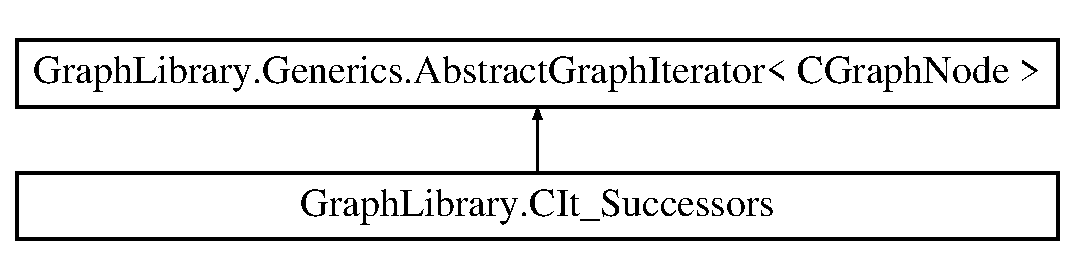
\includegraphics[height=2.000000cm]{class_graph_library_1_1_c_it___successors}
\end{center}
\end{figure}
\subsection*{Public Member Functions}
\begin{DoxyCompactItemize}
\item 
\hyperlink{class_graph_library_1_1_c_it___successors_afe5463ca23a259bb46b425f4f95b59c6}{C\+It\+\_\+\+Successors} (\hyperlink{class_graph_library_1_1_c_graph_node}{C\+Graph\+Node} node)
\begin{DoxyCompactList}\small\item\em Constructor. Takes the node to which iterator refers \end{DoxyCompactList}\item 
override \hyperlink{class_graph_library_1_1_c_graph_node}{C\+Graph\+Node} \hyperlink{class_graph_library_1_1_c_it___successors_ab13b972da76d0f8972114e8d376ba68c}{Begin} ()
\begin{DoxyCompactList}\small\item\em Points to the first valid item or to null if there is no one \end{DoxyCompactList}\item 
override bool \hyperlink{class_graph_library_1_1_c_it___successors_a8645c9047b2910e2c3bd246f8745773b}{End} ()
\begin{DoxyCompactList}\small\item\em \hyperlink{class_graph_library_1_1_c_it___successors_a8645c9047b2910e2c3bd246f8745773b}{End()} function runs after \hyperlink{class_graph_library_1_1_c_it___successors_ab13b972da76d0f8972114e8d376ba68c}{Begin()} and \hyperlink{class_graph_library_1_1_c_it___successors_abeba92b544a86d4385e9120289801df3}{Next()} functions and before we enter into the loop body. It validates that the iterator points to a proper item \end{DoxyCompactList}\item 
override \hyperlink{class_graph_library_1_1_c_graph_node}{C\+Graph\+Node} \hyperlink{class_graph_library_1_1_c_it___successors_abeba92b544a86d4385e9120289801df3}{Next} ()
\begin{DoxyCompactList}\small\item\em Points to the next valid item or to null if there isn\textquotesingle{}t one \end{DoxyCompactList}\end{DoxyCompactItemize}
\subsection*{Additional Inherited Members}


\subsection{Detailed Description}
Iterates over the native successor nodes of a node 



\subsection{Constructor \& Destructor Documentation}
\hypertarget{class_graph_library_1_1_c_it___successors_afe5463ca23a259bb46b425f4f95b59c6}{}\index{Graph\+Library\+::\+C\+It\+\_\+\+Successors@{Graph\+Library\+::\+C\+It\+\_\+\+Successors}!C\+It\+\_\+\+Successors@{C\+It\+\_\+\+Successors}}
\index{C\+It\+\_\+\+Successors@{C\+It\+\_\+\+Successors}!Graph\+Library\+::\+C\+It\+\_\+\+Successors@{Graph\+Library\+::\+C\+It\+\_\+\+Successors}}
\subsubsection[{C\+It\+\_\+\+Successors(\+C\+Graph\+Node node)}]{\setlength{\rightskip}{0pt plus 5cm}Graph\+Library.\+C\+It\+\_\+\+Successors.\+C\+It\+\_\+\+Successors (
\begin{DoxyParamCaption}
\item[{{\bf C\+Graph\+Node}}]{node}
\end{DoxyParamCaption}
)}\label{class_graph_library_1_1_c_it___successors_afe5463ca23a259bb46b425f4f95b59c6}


Constructor. Takes the node to which iterator refers 


\begin{DoxyParams}{Parameters}
{\em node} & Node to which the iterator is applied\\
\hline
\end{DoxyParams}


\subsection{Member Function Documentation}
\hypertarget{class_graph_library_1_1_c_it___successors_ab13b972da76d0f8972114e8d376ba68c}{}\index{Graph\+Library\+::\+C\+It\+\_\+\+Successors@{Graph\+Library\+::\+C\+It\+\_\+\+Successors}!Begin@{Begin}}
\index{Begin@{Begin}!Graph\+Library\+::\+C\+It\+\_\+\+Successors@{Graph\+Library\+::\+C\+It\+\_\+\+Successors}}
\subsubsection[{Begin()}]{\setlength{\rightskip}{0pt plus 5cm}override {\bf C\+Graph\+Node} Graph\+Library.\+C\+It\+\_\+\+Successors.\+Begin (
\begin{DoxyParamCaption}
{}
\end{DoxyParamCaption}
)\hspace{0.3cm}{\ttfamily [virtual]}}\label{class_graph_library_1_1_c_it___successors_ab13b972da76d0f8972114e8d376ba68c}


Points to the first valid item or to null if there is no one 

\begin{DoxyReturn}{Returns}

\end{DoxyReturn}


Implements \hyperlink{class_graph_library_1_1_generics_1_1_abstract_graph_iterator_a2c97c7a412c233b8442b7ad403f29779}{Graph\+Library.\+Generics.\+Abstract\+Graph\+Iterator$<$ C\+Graph\+Node $>$}.

\hypertarget{class_graph_library_1_1_c_it___successors_a8645c9047b2910e2c3bd246f8745773b}{}\index{Graph\+Library\+::\+C\+It\+\_\+\+Successors@{Graph\+Library\+::\+C\+It\+\_\+\+Successors}!End@{End}}
\index{End@{End}!Graph\+Library\+::\+C\+It\+\_\+\+Successors@{Graph\+Library\+::\+C\+It\+\_\+\+Successors}}
\subsubsection[{End()}]{\setlength{\rightskip}{0pt plus 5cm}override bool Graph\+Library.\+C\+It\+\_\+\+Successors.\+End (
\begin{DoxyParamCaption}
{}
\end{DoxyParamCaption}
)\hspace{0.3cm}{\ttfamily [virtual]}}\label{class_graph_library_1_1_c_it___successors_a8645c9047b2910e2c3bd246f8745773b}


\hyperlink{class_graph_library_1_1_c_it___successors_a8645c9047b2910e2c3bd246f8745773b}{End()} function runs after \hyperlink{class_graph_library_1_1_c_it___successors_ab13b972da76d0f8972114e8d376ba68c}{Begin()} and \hyperlink{class_graph_library_1_1_c_it___successors_abeba92b544a86d4385e9120289801df3}{Next()} functions and before we enter into the loop body. It validates that the iterator points to a proper item 

\begin{DoxyReturn}{Returns}

\end{DoxyReturn}


Implements \hyperlink{class_graph_library_1_1_generics_1_1_abstract_graph_iterator_aa8cd9f596ec0b6c4c1e9c244ba75df04}{Graph\+Library.\+Generics.\+Abstract\+Graph\+Iterator$<$ C\+Graph\+Node $>$}.

\hypertarget{class_graph_library_1_1_c_it___successors_abeba92b544a86d4385e9120289801df3}{}\index{Graph\+Library\+::\+C\+It\+\_\+\+Successors@{Graph\+Library\+::\+C\+It\+\_\+\+Successors}!Next@{Next}}
\index{Next@{Next}!Graph\+Library\+::\+C\+It\+\_\+\+Successors@{Graph\+Library\+::\+C\+It\+\_\+\+Successors}}
\subsubsection[{Next()}]{\setlength{\rightskip}{0pt plus 5cm}override {\bf C\+Graph\+Node} Graph\+Library.\+C\+It\+\_\+\+Successors.\+Next (
\begin{DoxyParamCaption}
{}
\end{DoxyParamCaption}
)\hspace{0.3cm}{\ttfamily [virtual]}}\label{class_graph_library_1_1_c_it___successors_abeba92b544a86d4385e9120289801df3}


Points to the next valid item or to null if there isn\textquotesingle{}t one 

\begin{DoxyReturn}{Returns}
Returns the current item
\end{DoxyReturn}


Implements \hyperlink{class_graph_library_1_1_generics_1_1_abstract_graph_iterator_aac8cffd0d579708a94ba056e4f4a00b2}{Graph\+Library.\+Generics.\+Abstract\+Graph\+Iterator$<$ C\+Graph\+Node $>$}.



The documentation for this class was generated from the following file\+:\begin{DoxyCompactItemize}
\item 
Graph\+Library/Graph\+Iterators.\+cs\end{DoxyCompactItemize}

\hypertarget{class_graph_library_1_1_aglorithms_1_1_edge_info___d_f_s}{}\section{Graph\+Library.\+Aglorithms.\+Edge\+Info\+\_\+\+D\+F\+S Class Reference}
\label{class_graph_library_1_1_aglorithms_1_1_edge_info___d_f_s}\index{Graph\+Library.\+Aglorithms.\+Edge\+Info\+\_\+\+D\+F\+S@{Graph\+Library.\+Aglorithms.\+Edge\+Info\+\_\+\+D\+F\+S}}


Graph edge info to assist the algorithm. There is an instance of the Info\+\_\+\+D\+F\+S class in each graph node  


Inheritance diagram for Graph\+Library.\+Aglorithms.\+Edge\+Info\+\_\+\+D\+F\+S\+:\begin{figure}[H]
\begin{center}
\leavevmode
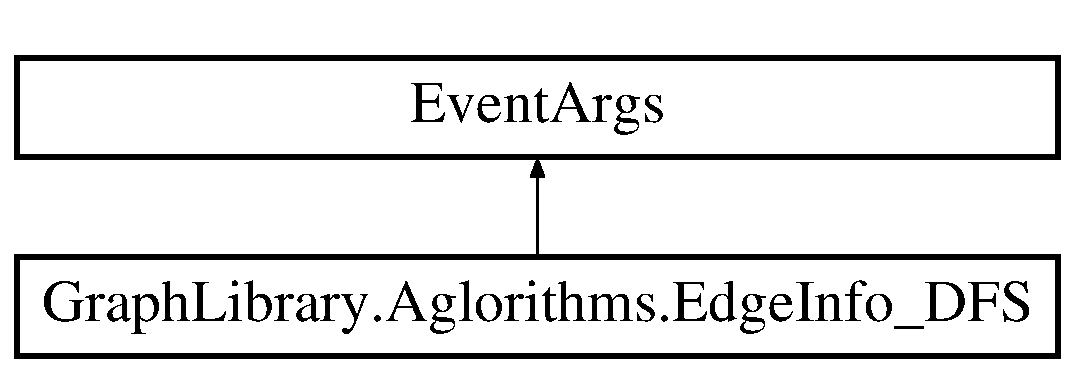
\includegraphics[height=2.000000cm]{class_graph_library_1_1_aglorithms_1_1_edge_info___d_f_s}
\end{center}
\end{figure}
\subsection*{Public Member Functions}
\begin{DoxyCompactItemize}
\item 
\hypertarget{class_graph_library_1_1_aglorithms_1_1_edge_info___d_f_s_a144cfb255ee900e143dfe729f946da8a}{}{\bfseries Edge\+Info\+\_\+\+D\+F\+S} (int color)\label{class_graph_library_1_1_aglorithms_1_1_edge_info___d_f_s_a144cfb255ee900e143dfe729f946da8a}

\end{DoxyCompactItemize}
\subsection*{Public Attributes}
\begin{DoxyCompactItemize}
\item 
\hypertarget{class_graph_library_1_1_aglorithms_1_1_edge_info___d_f_s_ad47e54c12b44b0ef0a34790139074389}{}int {\bfseries m\+\_\+color}\label{class_graph_library_1_1_aglorithms_1_1_edge_info___d_f_s_ad47e54c12b44b0ef0a34790139074389}

\end{DoxyCompactItemize}


\subsection{Detailed Description}
Graph edge info to assist the algorithm. There is an instance of the Info\+\_\+\+D\+F\+S class in each graph node 



The documentation for this class was generated from the following file\+:\begin{DoxyCompactItemize}
\item 
Graph\+Library/\+Aglorithms/Info\+\_\+\+D\+F\+S.\+cs\end{DoxyCompactItemize}

\hypertarget{class_graph_library_1_1_aglorithms_1_1_g_alg___edge_oriented_d_f_s}{}\section{Graph\+Library.\+Aglorithms.\+G\+Alg\+\_\+\+Edge\+Oriented\+D\+F\+S Class Reference}
\label{class_graph_library_1_1_aglorithms_1_1_g_alg___edge_oriented_d_f_s}\index{Graph\+Library.\+Aglorithms.\+G\+Alg\+\_\+\+Edge\+Oriented\+D\+F\+S@{Graph\+Library.\+Aglorithms.\+G\+Alg\+\_\+\+Edge\+Oriented\+D\+F\+S}}


This algorithm ( visitor ) performs a D\+F\+S traversal over a graph (directed or undirected ). It records the paths from which the algorithm passes by coloring nodes along them. The algorith works also for non-\/connected graphs 1) White (0) \+: Not yet visited 2) Gray (1) \+: Visited but not all of its neighbours 3) Black (2) \+: Visited and all of its neighbours  


Inheritance diagram for Graph\+Library.\+Aglorithms.\+G\+Alg\+\_\+\+Edge\+Oriented\+D\+F\+S\+:\begin{figure}[H]
\begin{center}
\leavevmode
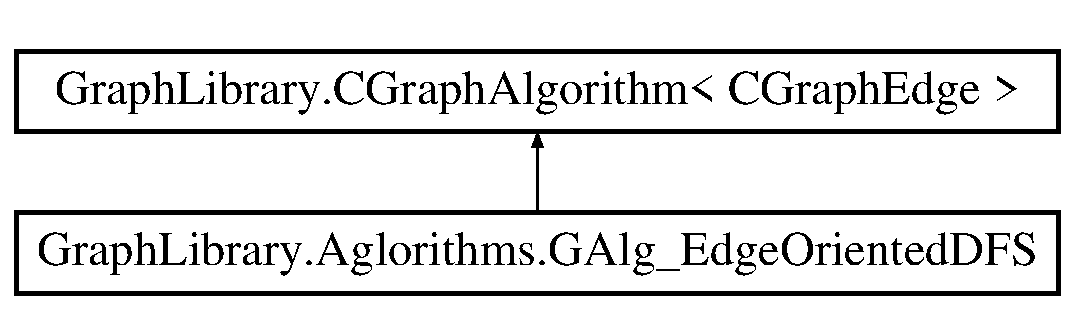
\includegraphics[height=2.000000cm]{class_graph_library_1_1_aglorithms_1_1_g_alg___edge_oriented_d_f_s}
\end{center}
\end{figure}
\subsection*{Public Member Functions}
\begin{DoxyCompactItemize}
\item 
\hyperlink{class_graph_library_1_1_aglorithms_1_1_g_alg___edge_oriented_d_f_s_ab154db21f7f5f64ec4d2899925a6c3bb}{G\+Alg\+\_\+\+Edge\+Oriented\+D\+F\+S} (\hyperlink{class_graph_library_1_1_c_graph}{C\+Graph} graph)
\begin{DoxyCompactList}\small\item\em Initializes a new instance of the \hyperlink{class_graph_library_1_1_aglorithms_1_1_g_alg___edge_oriented_d_f_s}{G\+Alg\+\_\+\+Edge\+Oriented\+D\+F\+S} class. \end{DoxyCompactList}\item 
\hypertarget{class_graph_library_1_1_aglorithms_1_1_g_alg___edge_oriented_d_f_s_aa0b0c46c857d02f7f93dc47ab8df7b5a}{}override void {\bfseries Init} ()\label{class_graph_library_1_1_aglorithms_1_1_g_alg___edge_oriented_d_f_s_aa0b0c46c857d02f7f93dc47ab8df7b5a}

\item 
override \hyperlink{class_graph_library_1_1_c_graph_edge}{C\+Graph\+Edge} \hyperlink{class_graph_library_1_1_aglorithms_1_1_g_alg___edge_oriented_d_f_s_ad46d1eec3b67f4fcd6ecdc02fb44603a}{Visit} (\hyperlink{class_graph_library_1_1_c_graph_edge}{C\+Graph\+Edge} edge)
\begin{DoxyCompactList}\small\item\em The Visit method refers to the action the algorithm performs to a specific edge Most of the times the Visit function is called recursively. \end{DoxyCompactList}\item 
int \hyperlink{class_graph_library_1_1_aglorithms_1_1_g_alg___edge_oriented_d_f_s_a99f99cba172890de22281af8c448fc1c}{Color} (\hyperlink{class_graph_library_1_1_c_graph_edge}{C\+Graph\+Edge} edge)
\begin{DoxyCompactList}\small\item\em Returns the color of the specified node \end{DoxyCompactList}\item 
void \hyperlink{class_graph_library_1_1_aglorithms_1_1_g_alg___edge_oriented_d_f_s_aeb59734bfbf42cdc8502e5b111d0a5b5}{Set\+Color} (\hyperlink{class_graph_library_1_1_c_graph_edge}{C\+Graph\+Edge} edge, int color)
\begin{DoxyCompactList}\small\item\em Sets the color of the specified node. \end{DoxyCompactList}\end{DoxyCompactItemize}
\subsection*{Additional Inherited Members}


\subsection{Detailed Description}
This algorithm ( visitor ) performs a D\+F\+S traversal over a graph (directed or undirected ). It records the paths from which the algorithm passes by coloring nodes along them. The algorith works also for non-\/connected graphs 1) White (0) \+: Not yet visited 2) Gray (1) \+: Visited but not all of its neighbours 3) Black (2) \+: Visited and all of its neighbours 



\subsection{Constructor \& Destructor Documentation}
\hypertarget{class_graph_library_1_1_aglorithms_1_1_g_alg___edge_oriented_d_f_s_ab154db21f7f5f64ec4d2899925a6c3bb}{}\index{Graph\+Library\+::\+Aglorithms\+::\+G\+Alg\+\_\+\+Edge\+Oriented\+D\+F\+S@{Graph\+Library\+::\+Aglorithms\+::\+G\+Alg\+\_\+\+Edge\+Oriented\+D\+F\+S}!G\+Alg\+\_\+\+Edge\+Oriented\+D\+F\+S@{G\+Alg\+\_\+\+Edge\+Oriented\+D\+F\+S}}
\index{G\+Alg\+\_\+\+Edge\+Oriented\+D\+F\+S@{G\+Alg\+\_\+\+Edge\+Oriented\+D\+F\+S}!Graph\+Library\+::\+Aglorithms\+::\+G\+Alg\+\_\+\+Edge\+Oriented\+D\+F\+S@{Graph\+Library\+::\+Aglorithms\+::\+G\+Alg\+\_\+\+Edge\+Oriented\+D\+F\+S}}
\subsubsection[{G\+Alg\+\_\+\+Edge\+Oriented\+D\+F\+S(\+C\+Graph graph)}]{\setlength{\rightskip}{0pt plus 5cm}Graph\+Library.\+Aglorithms.\+G\+Alg\+\_\+\+Edge\+Oriented\+D\+F\+S.\+G\+Alg\+\_\+\+Edge\+Oriented\+D\+F\+S (
\begin{DoxyParamCaption}
\item[{{\bf C\+Graph}}]{graph}
\end{DoxyParamCaption}
)}\label{class_graph_library_1_1_aglorithms_1_1_g_alg___edge_oriented_d_f_s_ab154db21f7f5f64ec4d2899925a6c3bb}


Initializes a new instance of the \hyperlink{class_graph_library_1_1_aglorithms_1_1_g_alg___edge_oriented_d_f_s}{G\+Alg\+\_\+\+Edge\+Oriented\+D\+F\+S} class. 


\begin{DoxyParams}{Parameters}
{\em graph} & The graph.\\
\hline
\end{DoxyParams}


\subsection{Member Function Documentation}
\hypertarget{class_graph_library_1_1_aglorithms_1_1_g_alg___edge_oriented_d_f_s_a99f99cba172890de22281af8c448fc1c}{}\index{Graph\+Library\+::\+Aglorithms\+::\+G\+Alg\+\_\+\+Edge\+Oriented\+D\+F\+S@{Graph\+Library\+::\+Aglorithms\+::\+G\+Alg\+\_\+\+Edge\+Oriented\+D\+F\+S}!Color@{Color}}
\index{Color@{Color}!Graph\+Library\+::\+Aglorithms\+::\+G\+Alg\+\_\+\+Edge\+Oriented\+D\+F\+S@{Graph\+Library\+::\+Aglorithms\+::\+G\+Alg\+\_\+\+Edge\+Oriented\+D\+F\+S}}
\subsubsection[{Color(\+C\+Graph\+Edge edge)}]{\setlength{\rightskip}{0pt plus 5cm}int Graph\+Library.\+Aglorithms.\+G\+Alg\+\_\+\+Edge\+Oriented\+D\+F\+S.\+Color (
\begin{DoxyParamCaption}
\item[{{\bf C\+Graph\+Edge}}]{edge}
\end{DoxyParamCaption}
)}\label{class_graph_library_1_1_aglorithms_1_1_g_alg___edge_oriented_d_f_s_a99f99cba172890de22281af8c448fc1c}


Returns the color of the specified node 


\begin{DoxyParams}{Parameters}
{\em node} & The node.\\
\hline
\end{DoxyParams}
\begin{DoxyReturn}{Returns}
\mbox{[}int\mbox{]}\+: Returns the color of the specified node 
\end{DoxyReturn}
\hypertarget{class_graph_library_1_1_aglorithms_1_1_g_alg___edge_oriented_d_f_s_aeb59734bfbf42cdc8502e5b111d0a5b5}{}\index{Graph\+Library\+::\+Aglorithms\+::\+G\+Alg\+\_\+\+Edge\+Oriented\+D\+F\+S@{Graph\+Library\+::\+Aglorithms\+::\+G\+Alg\+\_\+\+Edge\+Oriented\+D\+F\+S}!Set\+Color@{Set\+Color}}
\index{Set\+Color@{Set\+Color}!Graph\+Library\+::\+Aglorithms\+::\+G\+Alg\+\_\+\+Edge\+Oriented\+D\+F\+S@{Graph\+Library\+::\+Aglorithms\+::\+G\+Alg\+\_\+\+Edge\+Oriented\+D\+F\+S}}
\subsubsection[{Set\+Color(\+C\+Graph\+Edge edge, int color)}]{\setlength{\rightskip}{0pt plus 5cm}void Graph\+Library.\+Aglorithms.\+G\+Alg\+\_\+\+Edge\+Oriented\+D\+F\+S.\+Set\+Color (
\begin{DoxyParamCaption}
\item[{{\bf C\+Graph\+Edge}}]{edge, }
\item[{int}]{color}
\end{DoxyParamCaption}
)}\label{class_graph_library_1_1_aglorithms_1_1_g_alg___edge_oriented_d_f_s_aeb59734bfbf42cdc8502e5b111d0a5b5}


Sets the color of the specified node. 


\begin{DoxyParams}{Parameters}
{\em node} & The node.\\
\hline
{\em color} & The color.\\
\hline
\end{DoxyParams}
\hypertarget{class_graph_library_1_1_aglorithms_1_1_g_alg___edge_oriented_d_f_s_ad46d1eec3b67f4fcd6ecdc02fb44603a}{}\index{Graph\+Library\+::\+Aglorithms\+::\+G\+Alg\+\_\+\+Edge\+Oriented\+D\+F\+S@{Graph\+Library\+::\+Aglorithms\+::\+G\+Alg\+\_\+\+Edge\+Oriented\+D\+F\+S}!Visit@{Visit}}
\index{Visit@{Visit}!Graph\+Library\+::\+Aglorithms\+::\+G\+Alg\+\_\+\+Edge\+Oriented\+D\+F\+S@{Graph\+Library\+::\+Aglorithms\+::\+G\+Alg\+\_\+\+Edge\+Oriented\+D\+F\+S}}
\subsubsection[{Visit(\+C\+Graph\+Edge edge)}]{\setlength{\rightskip}{0pt plus 5cm}override {\bf C\+Graph\+Edge} Graph\+Library.\+Aglorithms.\+G\+Alg\+\_\+\+Edge\+Oriented\+D\+F\+S.\+Visit (
\begin{DoxyParamCaption}
\item[{{\bf C\+Graph\+Edge}}]{edge}
\end{DoxyParamCaption}
)}\label{class_graph_library_1_1_aglorithms_1_1_g_alg___edge_oriented_d_f_s_ad46d1eec3b67f4fcd6ecdc02fb44603a}


The Visit method refers to the action the algorithm performs to a specific edge Most of the times the Visit function is called recursively. 


\begin{DoxyParams}{Parameters}
{\em edge} & \\
\hline
\end{DoxyParams}
\begin{DoxyReturn}{Returns}
The parameter refers to the type of the return result 
\end{DoxyReturn}


The documentation for this class was generated from the following file\+:\begin{DoxyCompactItemize}
\item 
Graph\+Library/\+Aglorithms/G\+Alg\+\_\+\+Node\+Oriented\+D\+F\+S.\+cs\end{DoxyCompactItemize}

\hypertarget{class_graph_library_1_1_aglorithms_1_1_g_alg___node_oriented_d_f_s}{}\section{Graph\+Library.\+Aglorithms.\+G\+Alg\+\_\+\+Node\+Oriented\+D\+F\+S Class Reference}
\label{class_graph_library_1_1_aglorithms_1_1_g_alg___node_oriented_d_f_s}\index{Graph\+Library.\+Aglorithms.\+G\+Alg\+\_\+\+Node\+Oriented\+D\+F\+S@{Graph\+Library.\+Aglorithms.\+G\+Alg\+\_\+\+Node\+Oriented\+D\+F\+S}}


This algorithm ( visitor ) performs a D\+F\+S traversal over a graph (directed or undirected ). It records the paths from which the algorithm passes by coloring nodes along them. The algorith works also for non-\/connected graphs 1) White (0) \+: Not yet visited 2) Gray (1) \+: Visited but not all of its neighbours 3) Black (2) \+: Visited and all of its neighbours  


Inheritance diagram for Graph\+Library.\+Aglorithms.\+G\+Alg\+\_\+\+Node\+Oriented\+D\+F\+S\+:\begin{figure}[H]
\begin{center}
\leavevmode
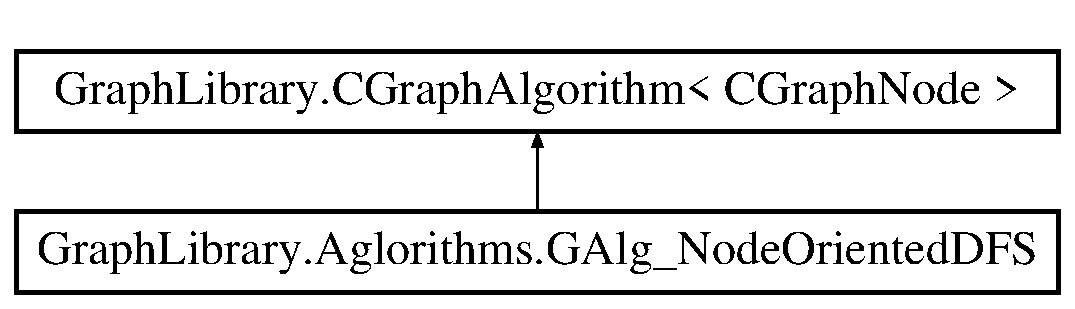
\includegraphics[height=2.000000cm]{class_graph_library_1_1_aglorithms_1_1_g_alg___node_oriented_d_f_s}
\end{center}
\end{figure}
\subsection*{Public Member Functions}
\begin{DoxyCompactItemize}
\item 
\hyperlink{class_graph_library_1_1_aglorithms_1_1_g_alg___node_oriented_d_f_s_a08a0b177dee71f014d5d2dfe929bae6c}{G\+Alg\+\_\+\+Node\+Oriented\+D\+F\+S} (\hyperlink{class_graph_library_1_1_c_graph}{C\+Graph} graph)
\begin{DoxyCompactList}\small\item\em Constructor \end{DoxyCompactList}\item 
\hypertarget{class_graph_library_1_1_aglorithms_1_1_g_alg___node_oriented_d_f_s_a67e72af02594968bea2c7c140bf55f4a}{}override void {\bfseries Init} ()\label{class_graph_library_1_1_aglorithms_1_1_g_alg___node_oriented_d_f_s_a67e72af02594968bea2c7c140bf55f4a}

\item 
\hypertarget{class_graph_library_1_1_aglorithms_1_1_g_alg___node_oriented_d_f_s_a27528338adca82162cdf706c70ddde42}{}override \hyperlink{class_graph_library_1_1_c_graph_node}{C\+Graph\+Node} {\bfseries Visit} (\hyperlink{class_graph_library_1_1_c_graph_node}{C\+Graph\+Node} node)\label{class_graph_library_1_1_aglorithms_1_1_g_alg___node_oriented_d_f_s_a27528338adca82162cdf706c70ddde42}

\item 
int \hyperlink{class_graph_library_1_1_aglorithms_1_1_g_alg___node_oriented_d_f_s_a33ee93fab673a0093497d2841fefb78d}{Color} (\hyperlink{class_graph_library_1_1_c_graph_node}{C\+Graph\+Node} node)
\begin{DoxyCompactList}\small\item\em Returns the color of the specified node \end{DoxyCompactList}\item 
void \hyperlink{class_graph_library_1_1_aglorithms_1_1_g_alg___node_oriented_d_f_s_aa6194f3209502e02fe32cd088a1d7e45}{Set\+Color} (\hyperlink{class_graph_library_1_1_c_graph_node}{C\+Graph\+Node} node, int color)
\begin{DoxyCompactList}\small\item\em Sets the color of the specified node. \end{DoxyCompactList}\item 
\hyperlink{class_graph_library_1_1_aglorithms_1_1_node_info___d_f_s}{Node\+Info\+\_\+\+D\+F\+S} \hyperlink{class_graph_library_1_1_aglorithms_1_1_g_alg___node_oriented_d_f_s_a55ad5132fce2173810b363f088f70003}{Node\+Info} (\hyperlink{class_graph_library_1_1_c_graph_node}{C\+Graph\+Node} node, object key)
\begin{DoxyCompactList}\small\item\em Returns the specified node information. \end{DoxyCompactList}\item 
\hypertarget{class_graph_library_1_1_aglorithms_1_1_g_alg___node_oriented_d_f_s_a10c4c01856895ec203cb5564169f38e0}{}void {\bfseries event\+Handler1} (object sender, Event\+Args arg)\label{class_graph_library_1_1_aglorithms_1_1_g_alg___node_oriented_d_f_s_a10c4c01856895ec203cb5564169f38e0}

\end{DoxyCompactItemize}
\subsection*{Properties}
\begin{DoxyCompactItemize}
\item 
bool \hyperlink{class_graph_library_1_1_aglorithms_1_1_g_alg___node_oriented_d_f_s_a7926a5bacfd6a50547e8848ead5b5a68}{M\+\_\+\+Start\+At\+Root\+Nodes}\hspace{0.3cm}{\ttfamily  \mbox{[}get, set\mbox{]}}
\begin{DoxyCompactList}\small\item\em Indicates whether the D\+F\+S start from nodes without predecessors \end{DoxyCompactList}\end{DoxyCompactItemize}
\subsection*{Events}
\begin{DoxyCompactItemize}
\item 
\hypertarget{class_graph_library_1_1_aglorithms_1_1_g_alg___node_oriented_d_f_s_a0075221ca2acf0374839e43f771e5c17}{}Event\+Handler {\bfseries m\+\_\+\+On\+Init}\label{class_graph_library_1_1_aglorithms_1_1_g_alg___node_oriented_d_f_s_a0075221ca2acf0374839e43f771e5c17}

\item 
\hypertarget{class_graph_library_1_1_aglorithms_1_1_g_alg___node_oriented_d_f_s_ab9102270aa7568fd3bf5abbde240385e}{}Event\+Handler {\bfseries m\+\_\+\+On\+Enter\+Node}\label{class_graph_library_1_1_aglorithms_1_1_g_alg___node_oriented_d_f_s_ab9102270aa7568fd3bf5abbde240385e}

\item 
\hypertarget{class_graph_library_1_1_aglorithms_1_1_g_alg___node_oriented_d_f_s_a7a2e9dd262f27b2cfa97092224de4025}{}Event\+Handler {\bfseries m\+\_\+\+On\+Exit\+Node}\label{class_graph_library_1_1_aglorithms_1_1_g_alg___node_oriented_d_f_s_a7a2e9dd262f27b2cfa97092224de4025}

\item 
\hypertarget{class_graph_library_1_1_aglorithms_1_1_g_alg___node_oriented_d_f_s_a782cb35a1823fa98dcbaaaaae376e214}{}Event\+Handler {\bfseries m\+\_\+\+On\+Bypassing\+Node}\label{class_graph_library_1_1_aglorithms_1_1_g_alg___node_oriented_d_f_s_a782cb35a1823fa98dcbaaaaae376e214}

\end{DoxyCompactItemize}
\subsection*{Additional Inherited Members}


\subsection{Detailed Description}
This algorithm ( visitor ) performs a D\+F\+S traversal over a graph (directed or undirected ). It records the paths from which the algorithm passes by coloring nodes along them. The algorith works also for non-\/connected graphs 1) White (0) \+: Not yet visited 2) Gray (1) \+: Visited but not all of its neighbours 3) Black (2) \+: Visited and all of its neighbours 



\subsection{Constructor \& Destructor Documentation}
\hypertarget{class_graph_library_1_1_aglorithms_1_1_g_alg___node_oriented_d_f_s_a08a0b177dee71f014d5d2dfe929bae6c}{}\index{Graph\+Library\+::\+Aglorithms\+::\+G\+Alg\+\_\+\+Node\+Oriented\+D\+F\+S@{Graph\+Library\+::\+Aglorithms\+::\+G\+Alg\+\_\+\+Node\+Oriented\+D\+F\+S}!G\+Alg\+\_\+\+Node\+Oriented\+D\+F\+S@{G\+Alg\+\_\+\+Node\+Oriented\+D\+F\+S}}
\index{G\+Alg\+\_\+\+Node\+Oriented\+D\+F\+S@{G\+Alg\+\_\+\+Node\+Oriented\+D\+F\+S}!Graph\+Library\+::\+Aglorithms\+::\+G\+Alg\+\_\+\+Node\+Oriented\+D\+F\+S@{Graph\+Library\+::\+Aglorithms\+::\+G\+Alg\+\_\+\+Node\+Oriented\+D\+F\+S}}
\subsubsection[{G\+Alg\+\_\+\+Node\+Oriented\+D\+F\+S(\+C\+Graph graph)}]{\setlength{\rightskip}{0pt plus 5cm}Graph\+Library.\+Aglorithms.\+G\+Alg\+\_\+\+Node\+Oriented\+D\+F\+S.\+G\+Alg\+\_\+\+Node\+Oriented\+D\+F\+S (
\begin{DoxyParamCaption}
\item[{{\bf C\+Graph}}]{graph}
\end{DoxyParamCaption}
)}\label{class_graph_library_1_1_aglorithms_1_1_g_alg___node_oriented_d_f_s_a08a0b177dee71f014d5d2dfe929bae6c}


Constructor 


\begin{DoxyParams}{Parameters}
{\em graph} & Graph to which the algorithm is applied\\
\hline
\end{DoxyParams}


\subsection{Member Function Documentation}
\hypertarget{class_graph_library_1_1_aglorithms_1_1_g_alg___node_oriented_d_f_s_a33ee93fab673a0093497d2841fefb78d}{}\index{Graph\+Library\+::\+Aglorithms\+::\+G\+Alg\+\_\+\+Node\+Oriented\+D\+F\+S@{Graph\+Library\+::\+Aglorithms\+::\+G\+Alg\+\_\+\+Node\+Oriented\+D\+F\+S}!Color@{Color}}
\index{Color@{Color}!Graph\+Library\+::\+Aglorithms\+::\+G\+Alg\+\_\+\+Node\+Oriented\+D\+F\+S@{Graph\+Library\+::\+Aglorithms\+::\+G\+Alg\+\_\+\+Node\+Oriented\+D\+F\+S}}
\subsubsection[{Color(\+C\+Graph\+Node node)}]{\setlength{\rightskip}{0pt plus 5cm}int Graph\+Library.\+Aglorithms.\+G\+Alg\+\_\+\+Node\+Oriented\+D\+F\+S.\+Color (
\begin{DoxyParamCaption}
\item[{{\bf C\+Graph\+Node}}]{node}
\end{DoxyParamCaption}
)}\label{class_graph_library_1_1_aglorithms_1_1_g_alg___node_oriented_d_f_s_a33ee93fab673a0093497d2841fefb78d}


Returns the color of the specified node 


\begin{DoxyParams}{Parameters}
{\em node} & The node.\\
\hline
\end{DoxyParams}
\begin{DoxyReturn}{Returns}
\mbox{[}int\mbox{]}\+: Returns the color of the specified node 
\end{DoxyReturn}
\hypertarget{class_graph_library_1_1_aglorithms_1_1_g_alg___node_oriented_d_f_s_a55ad5132fce2173810b363f088f70003}{}\index{Graph\+Library\+::\+Aglorithms\+::\+G\+Alg\+\_\+\+Node\+Oriented\+D\+F\+S@{Graph\+Library\+::\+Aglorithms\+::\+G\+Alg\+\_\+\+Node\+Oriented\+D\+F\+S}!Node\+Info@{Node\+Info}}
\index{Node\+Info@{Node\+Info}!Graph\+Library\+::\+Aglorithms\+::\+G\+Alg\+\_\+\+Node\+Oriented\+D\+F\+S@{Graph\+Library\+::\+Aglorithms\+::\+G\+Alg\+\_\+\+Node\+Oriented\+D\+F\+S}}
\subsubsection[{Node\+Info(\+C\+Graph\+Node node, object key)}]{\setlength{\rightskip}{0pt plus 5cm}{\bf Node\+Info\+\_\+\+D\+F\+S} Graph\+Library.\+Aglorithms.\+G\+Alg\+\_\+\+Node\+Oriented\+D\+F\+S.\+Node\+Info (
\begin{DoxyParamCaption}
\item[{{\bf C\+Graph\+Node}}]{node, }
\item[{object}]{key}
\end{DoxyParamCaption}
)}\label{class_graph_library_1_1_aglorithms_1_1_g_alg___node_oriented_d_f_s_a55ad5132fce2173810b363f088f70003}


Returns the specified node information. 


\begin{DoxyParams}{Parameters}
{\em node} & The node.\\
\hline
{\em key} & The key.\\
\hline
\end{DoxyParams}
\begin{DoxyReturn}{Returns}

\end{DoxyReturn}
\hypertarget{class_graph_library_1_1_aglorithms_1_1_g_alg___node_oriented_d_f_s_aa6194f3209502e02fe32cd088a1d7e45}{}\index{Graph\+Library\+::\+Aglorithms\+::\+G\+Alg\+\_\+\+Node\+Oriented\+D\+F\+S@{Graph\+Library\+::\+Aglorithms\+::\+G\+Alg\+\_\+\+Node\+Oriented\+D\+F\+S}!Set\+Color@{Set\+Color}}
\index{Set\+Color@{Set\+Color}!Graph\+Library\+::\+Aglorithms\+::\+G\+Alg\+\_\+\+Node\+Oriented\+D\+F\+S@{Graph\+Library\+::\+Aglorithms\+::\+G\+Alg\+\_\+\+Node\+Oriented\+D\+F\+S}}
\subsubsection[{Set\+Color(\+C\+Graph\+Node node, int color)}]{\setlength{\rightskip}{0pt plus 5cm}void Graph\+Library.\+Aglorithms.\+G\+Alg\+\_\+\+Node\+Oriented\+D\+F\+S.\+Set\+Color (
\begin{DoxyParamCaption}
\item[{{\bf C\+Graph\+Node}}]{node, }
\item[{int}]{color}
\end{DoxyParamCaption}
)}\label{class_graph_library_1_1_aglorithms_1_1_g_alg___node_oriented_d_f_s_aa6194f3209502e02fe32cd088a1d7e45}


Sets the color of the specified node. 


\begin{DoxyParams}{Parameters}
{\em node} & The node.\\
\hline
{\em color} & The color.\\
\hline
\end{DoxyParams}


\subsection{Property Documentation}
\hypertarget{class_graph_library_1_1_aglorithms_1_1_g_alg___node_oriented_d_f_s_a7926a5bacfd6a50547e8848ead5b5a68}{}\index{Graph\+Library\+::\+Aglorithms\+::\+G\+Alg\+\_\+\+Node\+Oriented\+D\+F\+S@{Graph\+Library\+::\+Aglorithms\+::\+G\+Alg\+\_\+\+Node\+Oriented\+D\+F\+S}!M\+\_\+\+Start\+At\+Root\+Nodes@{M\+\_\+\+Start\+At\+Root\+Nodes}}
\index{M\+\_\+\+Start\+At\+Root\+Nodes@{M\+\_\+\+Start\+At\+Root\+Nodes}!Graph\+Library\+::\+Aglorithms\+::\+G\+Alg\+\_\+\+Node\+Oriented\+D\+F\+S@{Graph\+Library\+::\+Aglorithms\+::\+G\+Alg\+\_\+\+Node\+Oriented\+D\+F\+S}}
\subsubsection[{M\+\_\+\+Start\+At\+Root\+Nodes}]{\setlength{\rightskip}{0pt plus 5cm}bool Graph\+Library.\+Aglorithms.\+G\+Alg\+\_\+\+Node\+Oriented\+D\+F\+S.\+M\+\_\+\+Start\+At\+Root\+Nodes\hspace{0.3cm}{\ttfamily [get]}, {\ttfamily [set]}}\label{class_graph_library_1_1_aglorithms_1_1_g_alg___node_oriented_d_f_s_a7926a5bacfd6a50547e8848ead5b5a68}


Indicates whether the D\+F\+S start from nodes without predecessors 

{\ttfamily true} if the algorithm starts at nodes without predecessors; otherwise, {\ttfamily false}. 

The documentation for this class was generated from the following file\+:\begin{DoxyCompactItemize}
\item 
Graph\+Library/\+Aglorithms/G\+Alg\+\_\+\+Node\+Oriented\+D\+F\+S.\+cs\end{DoxyCompactItemize}

\hypertarget{class_graph_library_1_1_printers_1_1_graph_viz_printer_1_1_graph_viz_node_labeling}{}\section{Graph\+Library.\+Printers.\+Graph\+Viz\+Printer.\+Graph\+Viz\+Node\+Labeling Class Reference}
\label{class_graph_library_1_1_printers_1_1_graph_viz_printer_1_1_graph_viz_node_labeling}\index{Graph\+Library.\+Printers.\+Graph\+Viz\+Printer.\+Graph\+Viz\+Node\+Labeling@{Graph\+Library.\+Printers.\+Graph\+Viz\+Printer.\+Graph\+Viz\+Node\+Labeling}}


Assign labels to nodes for graphviz printing  


Inheritance diagram for Graph\+Library.\+Printers.\+Graph\+Viz\+Printer.\+Graph\+Viz\+Node\+Labeling\+:\begin{figure}[H]
\begin{center}
\leavevmode
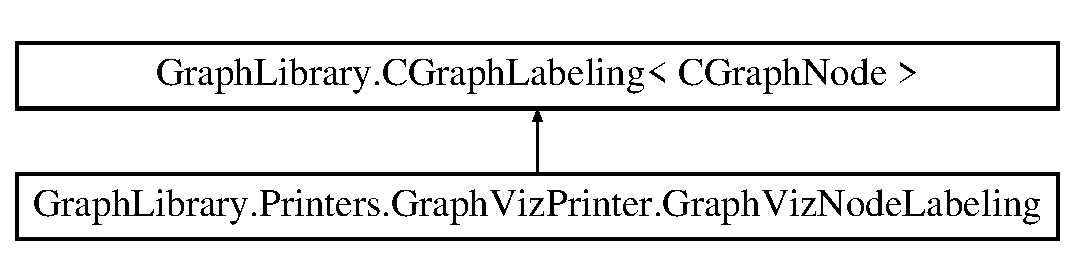
\includegraphics[height=2.000000cm]{class_graph_library_1_1_printers_1_1_graph_viz_printer_1_1_graph_viz_node_labeling}
\end{center}
\end{figure}
\subsection*{Public Member Functions}
\begin{DoxyCompactItemize}
\item 
\hyperlink{class_graph_library_1_1_printers_1_1_graph_viz_printer_1_1_graph_viz_node_labeling_ac9d3114f90663140e34050c62cd90497}{Graph\+Viz\+Node\+Labeling} (\hyperlink{class_graph_library_1_1_c_graph}{C\+Graph} graph)
\begin{DoxyCompactList}\small\item\em Initializes a new instance of the \hyperlink{class_graph_library_1_1_printers_1_1_graph_viz_printer_1_1_graph_viz_node_labeling}{Graph\+Viz\+Node\+Labeling} class. \end{DoxyCompactList}\end{DoxyCompactItemize}
\subsection*{Protected Member Functions}
\begin{DoxyCompactItemize}
\item 
override void \hyperlink{class_graph_library_1_1_printers_1_1_graph_viz_printer_1_1_graph_viz_node_labeling_a5e6ecfffa91b069313f4e2b319b9a48c}{Label\+Elements} ()
\begin{DoxyCompactList}\small\item\em Gives the initial mapping of labels to elements. Called by the constructor. Must be defined in subclasses \end{DoxyCompactList}\end{DoxyCompactItemize}
\subsection*{Additional Inherited Members}


\subsection{Detailed Description}
Assign labels to nodes for graphviz printing 

\begin{DoxySeeAlso}{See also}
\hyperlink{class_graph_library_1_1_c_graph_node}{C\+Graph\+Node}


\end{DoxySeeAlso}


\subsection{Constructor \& Destructor Documentation}
\hypertarget{class_graph_library_1_1_printers_1_1_graph_viz_printer_1_1_graph_viz_node_labeling_ac9d3114f90663140e34050c62cd90497}{}\index{Graph\+Library\+::\+Printers\+::\+Graph\+Viz\+Printer\+::\+Graph\+Viz\+Node\+Labeling@{Graph\+Library\+::\+Printers\+::\+Graph\+Viz\+Printer\+::\+Graph\+Viz\+Node\+Labeling}!Graph\+Viz\+Node\+Labeling@{Graph\+Viz\+Node\+Labeling}}
\index{Graph\+Viz\+Node\+Labeling@{Graph\+Viz\+Node\+Labeling}!Graph\+Library\+::\+Printers\+::\+Graph\+Viz\+Printer\+::\+Graph\+Viz\+Node\+Labeling@{Graph\+Library\+::\+Printers\+::\+Graph\+Viz\+Printer\+::\+Graph\+Viz\+Node\+Labeling}}
\subsubsection[{Graph\+Viz\+Node\+Labeling(\+C\+Graph graph)}]{\setlength{\rightskip}{0pt plus 5cm}Graph\+Library.\+Printers.\+Graph\+Viz\+Printer.\+Graph\+Viz\+Node\+Labeling.\+Graph\+Viz\+Node\+Labeling (
\begin{DoxyParamCaption}
\item[{{\bf C\+Graph}}]{graph}
\end{DoxyParamCaption}
)}\label{class_graph_library_1_1_printers_1_1_graph_viz_printer_1_1_graph_viz_node_labeling_ac9d3114f90663140e34050c62cd90497}


Initializes a new instance of the \hyperlink{class_graph_library_1_1_printers_1_1_graph_viz_printer_1_1_graph_viz_node_labeling}{Graph\+Viz\+Node\+Labeling} class. 


\begin{DoxyParams}{Parameters}
{\em graph} & The graph.\\
\hline
\end{DoxyParams}


\subsection{Member Function Documentation}
\hypertarget{class_graph_library_1_1_printers_1_1_graph_viz_printer_1_1_graph_viz_node_labeling_a5e6ecfffa91b069313f4e2b319b9a48c}{}\index{Graph\+Library\+::\+Printers\+::\+Graph\+Viz\+Printer\+::\+Graph\+Viz\+Node\+Labeling@{Graph\+Library\+::\+Printers\+::\+Graph\+Viz\+Printer\+::\+Graph\+Viz\+Node\+Labeling}!Label\+Elements@{Label\+Elements}}
\index{Label\+Elements@{Label\+Elements}!Graph\+Library\+::\+Printers\+::\+Graph\+Viz\+Printer\+::\+Graph\+Viz\+Node\+Labeling@{Graph\+Library\+::\+Printers\+::\+Graph\+Viz\+Printer\+::\+Graph\+Viz\+Node\+Labeling}}
\subsubsection[{Label\+Elements()}]{\setlength{\rightskip}{0pt plus 5cm}override void Graph\+Library.\+Printers.\+Graph\+Viz\+Printer.\+Graph\+Viz\+Node\+Labeling.\+Label\+Elements (
\begin{DoxyParamCaption}
{}
\end{DoxyParamCaption}
)\hspace{0.3cm}{\ttfamily [protected]}}\label{class_graph_library_1_1_printers_1_1_graph_viz_printer_1_1_graph_viz_node_labeling_a5e6ecfffa91b069313f4e2b319b9a48c}


Gives the initial mapping of labels to elements. Called by the constructor. Must be defined in subclasses 



The documentation for this class was generated from the following file\+:\begin{DoxyCompactItemize}
\item 
Graph\+Library/\+Printers/\+Graph\+Viz\+Printer/Graph\+Viz\+Labeling.\+cs\end{DoxyCompactItemize}

\hypertarget{interface_graph_library_1_1_generics_1_1_i_graph_algorithm}{}\section{Graph\+Library.\+Generics.\+I\+Graph\+Algorithm$<$ T, T\+Node $>$ Interface Template Reference}
\label{interface_graph_library_1_1_generics_1_1_i_graph_algorithm}\index{Graph\+Library.\+Generics.\+I\+Graph\+Algorithm$<$ T, T\+Node $>$@{Graph\+Library.\+Generics.\+I\+Graph\+Algorithm$<$ T, T\+Node $>$}}


The interface represent the mandatory interface of the algorithm class.  


Inheritance diagram for Graph\+Library.\+Generics.\+I\+Graph\+Algorithm$<$ T, T\+Node $>$\+:\begin{figure}[H]
\begin{center}
\leavevmode
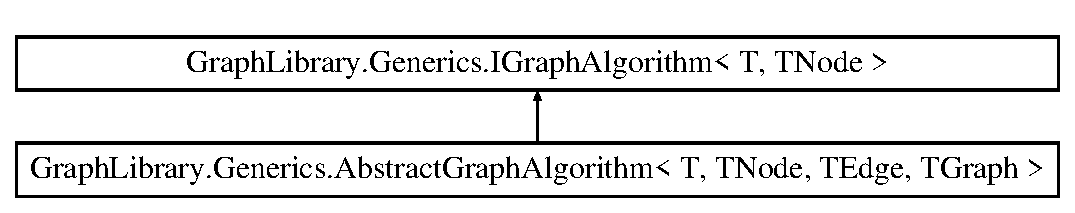
\includegraphics[height=2.000000cm]{interface_graph_library_1_1_generics_1_1_i_graph_algorithm}
\end{center}
\end{figure}
\subsection*{Public Member Functions}
\begin{DoxyCompactItemize}
\item 
T \hyperlink{interface_graph_library_1_1_generics_1_1_i_graph_algorithm_a8bc65da7e1004a5c55f75b57872fad31}{Visit} (T\+Node node)
\begin{DoxyCompactList}\small\item\em The Visit method refers to the action the algorithm performs to a specific node Visit function can be called recursively or iteratively. \end{DoxyCompactList}\item 
object \hyperlink{interface_graph_library_1_1_generics_1_1_i_graph_algorithm_aa8576b6860d0047bfd491c3101e876cc}{Visit\+Children} (T\+Node node)
\begin{DoxyCompactList}\small\item\em Visits the children of the specified node. \end{DoxyCompactList}\end{DoxyCompactItemize}


\subsection{Detailed Description}
The interface represent the mandatory interface of the algorithm class. 


\begin{DoxyTemplParams}{Template Parameters}
{\em T} & The parameter refers to the type of the return result\\
\hline
{\em Node} & The type of the node.\\
\hline
\end{DoxyTemplParams}


\subsection{Member Function Documentation}
\hypertarget{interface_graph_library_1_1_generics_1_1_i_graph_algorithm_a8bc65da7e1004a5c55f75b57872fad31}{}\index{Graph\+Library\+::\+Generics\+::\+I\+Graph\+Algorithm@{Graph\+Library\+::\+Generics\+::\+I\+Graph\+Algorithm}!Visit@{Visit}}
\index{Visit@{Visit}!Graph\+Library\+::\+Generics\+::\+I\+Graph\+Algorithm@{Graph\+Library\+::\+Generics\+::\+I\+Graph\+Algorithm}}
\subsubsection[{Visit(\+T\+Node node)}]{\setlength{\rightskip}{0pt plus 5cm}T {\bf Graph\+Library.\+Generics.\+I\+Graph\+Algorithm}$<$ T, T\+Node $>$.Visit (
\begin{DoxyParamCaption}
\item[{T\+Node}]{node}
\end{DoxyParamCaption}
)}\label{interface_graph_library_1_1_generics_1_1_i_graph_algorithm_a8bc65da7e1004a5c55f75b57872fad31}


The Visit method refers to the action the algorithm performs to a specific node Visit function can be called recursively or iteratively. 


\begin{DoxyParams}{Parameters}
{\em node} & The node to which the algorithm acts.\\
\hline
\end{DoxyParams}
\begin{DoxyReturn}{Returns}
The parameter refers to the type of the return result
\end{DoxyReturn}


Implemented in \hyperlink{class_graph_library_1_1_generics_1_1_abstract_graph_algorithm_a08ce42bc60d311959bc5d1293d3c63da}{Graph\+Library.\+Generics.\+Abstract\+Graph\+Algorithm$<$ T, T\+Node, T\+Edge, T\+Graph $>$}.

\hypertarget{interface_graph_library_1_1_generics_1_1_i_graph_algorithm_aa8576b6860d0047bfd491c3101e876cc}{}\index{Graph\+Library\+::\+Generics\+::\+I\+Graph\+Algorithm@{Graph\+Library\+::\+Generics\+::\+I\+Graph\+Algorithm}!Visit\+Children@{Visit\+Children}}
\index{Visit\+Children@{Visit\+Children}!Graph\+Library\+::\+Generics\+::\+I\+Graph\+Algorithm@{Graph\+Library\+::\+Generics\+::\+I\+Graph\+Algorithm}}
\subsubsection[{Visit\+Children(\+T\+Node node)}]{\setlength{\rightskip}{0pt plus 5cm}object {\bf Graph\+Library.\+Generics.\+I\+Graph\+Algorithm}$<$ T, T\+Node $>$.Visit\+Children (
\begin{DoxyParamCaption}
\item[{T\+Node}]{node}
\end{DoxyParamCaption}
)}\label{interface_graph_library_1_1_generics_1_1_i_graph_algorithm_aa8576b6860d0047bfd491c3101e876cc}


Visits the children of the specified node. 


\begin{DoxyParams}{Parameters}
{\em node} & The node to which the children is visited\\
\hline
\end{DoxyParams}
\begin{DoxyReturn}{Returns}
an object of type object
\end{DoxyReturn}


Implemented in \hyperlink{class_graph_library_1_1_generics_1_1_abstract_graph_algorithm_afe8f7c1f5bf5085b31a59139d6034eba}{Graph\+Library.\+Generics.\+Abstract\+Graph\+Algorithm$<$ T, T\+Node, T\+Edge, T\+Graph $>$}.



The documentation for this interface was generated from the following file\+:\begin{DoxyCompactItemize}
\item 
Graph\+Library/\+Generics/Abstract\+Graph\+Algorithm.\+cs\end{DoxyCompactItemize}

\hypertarget{interface_graph_library_1_1_generics_1_1_i_graph_iterator}{}\section{Graph\+Library.\+Generics.\+I\+Graph\+Iterator$<$ T $>$ Interface Template Reference}
\label{interface_graph_library_1_1_generics_1_1_i_graph_iterator}\index{Graph\+Library.\+Generics.\+I\+Graph\+Iterator$<$ T $>$@{Graph\+Library.\+Generics.\+I\+Graph\+Iterator$<$ T $>$}}


Every iterator should implement the following interface. Look for more details in the \begin{DoxySeeAlso}{See also}
\hyperlink{class_graph_library_1_1_generics_1_1_abstract_graph_iterator}{Abstract\+Graph\+Iterator}


\end{DoxySeeAlso}
class  


Inheritance diagram for Graph\+Library.\+Generics.\+I\+Graph\+Iterator$<$ T $>$\+:\begin{figure}[H]
\begin{center}
\leavevmode
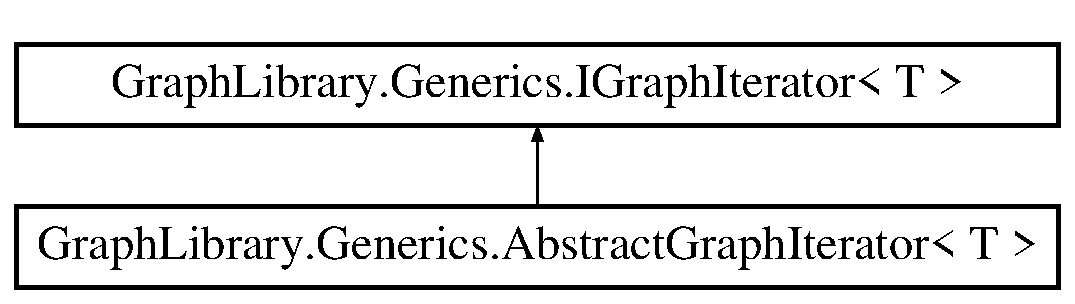
\includegraphics[height=2.000000cm]{interface_graph_library_1_1_generics_1_1_i_graph_iterator}
\end{center}
\end{figure}
\subsection*{Public Member Functions}
\begin{DoxyCompactItemize}
\item 
\hypertarget{interface_graph_library_1_1_generics_1_1_i_graph_iterator_ac05f3892ce9ada56e29b97af0a16b624}{}T {\bfseries Begin} ()\label{interface_graph_library_1_1_generics_1_1_i_graph_iterator_ac05f3892ce9ada56e29b97af0a16b624}

\item 
\hypertarget{interface_graph_library_1_1_generics_1_1_i_graph_iterator_a07079326b0d3a2fc539357140321f2fe}{}bool {\bfseries End} ()\label{interface_graph_library_1_1_generics_1_1_i_graph_iterator_a07079326b0d3a2fc539357140321f2fe}

\item 
\hypertarget{interface_graph_library_1_1_generics_1_1_i_graph_iterator_ad3b9494de0793a30b5ac5678f769e000}{}T {\bfseries Next} ()\label{interface_graph_library_1_1_generics_1_1_i_graph_iterator_ad3b9494de0793a30b5ac5678f769e000}

\end{DoxyCompactItemize}


\subsection{Detailed Description}
Every iterator should implement the following interface. Look for more details in the \begin{DoxySeeAlso}{See also}
\hyperlink{class_graph_library_1_1_generics_1_1_abstract_graph_iterator}{Abstract\+Graph\+Iterator}


\end{DoxySeeAlso}
class 


\begin{DoxyTemplParams}{Template Parameters}
{\em T} & The type of elements that this iterator iterates on\\
\hline
\end{DoxyTemplParams}


The documentation for this interface was generated from the following file\+:\begin{DoxyCompactItemize}
\item 
Graph\+Library/\+Generics/Abstract\+Graph\+Iterators.\+cs\end{DoxyCompactItemize}

\hypertarget{interface_graph_library_1_1_generics_1_1_i_graph_labeling}{}\section{Graph\+Library.\+Generics.\+I\+Graph\+Labeling$<$ T $>$ Interface Template Reference}
\label{interface_graph_library_1_1_generics_1_1_i_graph_labeling}\index{Graph\+Library.\+Generics.\+I\+Graph\+Labeling$<$ T $>$@{Graph\+Library.\+Generics.\+I\+Graph\+Labeling$<$ T $>$}}


Provides a generic interface for retrieving the label of a graph element of type T ( edge, node, whatever... ). Thus this class applies to all types of graph elements.  


\subsection*{Public Member Functions}
\begin{DoxyCompactItemize}
\item 
string \hyperlink{interface_graph_library_1_1_generics_1_1_i_graph_labeling_a2904d32c62f983b7afd6703ba8922a7b}{Label} (T element)
\begin{DoxyCompactList}\small\item\em Returns the Label of the specified element. \end{DoxyCompactList}\item 
string \hyperlink{interface_graph_library_1_1_generics_1_1_i_graph_labeling_a9f5aa9fd0ae47e9ba13845eb3ca71fe3}{Label} (int serial\+Number)
\begin{DoxyCompactList}\small\item\em Returns the Label of the element with the given serial number. \end{DoxyCompactList}\item 
T \hyperlink{interface_graph_library_1_1_generics_1_1_i_graph_labeling_a4d45b0ba9ac709dcabadab1d69cef8f1}{Element} (string label)
\begin{DoxyCompactList}\small\item\em Returns the element that is labelled with the given label \end{DoxyCompactList}\item 
void \hyperlink{interface_graph_library_1_1_generics_1_1_i_graph_labeling_a46bec4e7f765d5e6ede5e758cee4145a}{Set\+Label} (T element, string label)
\begin{DoxyCompactList}\small\item\em Sets the label of the given element. The element must exist in the graph and the label must not be already used by another element of the same type (node, edge) \end{DoxyCompactList}\item 
void \hyperlink{interface_graph_library_1_1_generics_1_1_i_graph_labeling_ab5abcba5824c65ffb695aba813b06a8e}{Set\+Label} (int serial\+Number, \hyperlink{namespace_graph_library_1_1_generics_a919a165f16deccdd1b3d7e8a93423fbc}{Graph\+Element\+Type} element\+Type, string label)
\begin{DoxyCompactList}\small\item\em Sets the label of the element with the given serialnumber and type. The element must exist in the graph and the label must not be already used by another element of the same type (node, edge) \end{DoxyCompactList}\end{DoxyCompactItemize}


\subsection{Detailed Description}
Provides a generic interface for retrieving the label of a graph element of type T ( edge, node, whatever... ). Thus this class applies to all types of graph elements. 


\begin{DoxyTemplParams}{Template Parameters}
{\em T} & The type of graph element\\
\hline
\end{DoxyTemplParams}
\begin{Desc}
\item[Type Constraints]\begin{description}
\item[{\em T} : {\em \hyperlink{interface_graph_library_1_1_generics_1_1_i_graph_primitive}{I\+Graph\+Primitive}}]\end{description}
\end{Desc}


\subsection{Member Function Documentation}
\hypertarget{interface_graph_library_1_1_generics_1_1_i_graph_labeling_a4d45b0ba9ac709dcabadab1d69cef8f1}{}\index{Graph\+Library\+::\+Generics\+::\+I\+Graph\+Labeling@{Graph\+Library\+::\+Generics\+::\+I\+Graph\+Labeling}!Element@{Element}}
\index{Element@{Element}!Graph\+Library\+::\+Generics\+::\+I\+Graph\+Labeling@{Graph\+Library\+::\+Generics\+::\+I\+Graph\+Labeling}}
\subsubsection[{Element(string label)}]{\setlength{\rightskip}{0pt plus 5cm}T {\bf Graph\+Library.\+Generics.\+I\+Graph\+Labeling}$<$ T $>$.Element (
\begin{DoxyParamCaption}
\item[{string}]{label}
\end{DoxyParamCaption}
)}\label{interface_graph_library_1_1_generics_1_1_i_graph_labeling_a4d45b0ba9ac709dcabadab1d69cef8f1}


Returns the element that is labelled with the given label 


\begin{DoxyParams}{Parameters}
{\em label} & The label\\
\hline
\end{DoxyParams}
\begin{DoxyReturn}{Returns}
The element
\end{DoxyReturn}
\hypertarget{interface_graph_library_1_1_generics_1_1_i_graph_labeling_a2904d32c62f983b7afd6703ba8922a7b}{}\index{Graph\+Library\+::\+Generics\+::\+I\+Graph\+Labeling@{Graph\+Library\+::\+Generics\+::\+I\+Graph\+Labeling}!Label@{Label}}
\index{Label@{Label}!Graph\+Library\+::\+Generics\+::\+I\+Graph\+Labeling@{Graph\+Library\+::\+Generics\+::\+I\+Graph\+Labeling}}
\subsubsection[{Label(\+T element)}]{\setlength{\rightskip}{0pt plus 5cm}string {\bf Graph\+Library.\+Generics.\+I\+Graph\+Labeling}$<$ T $>$.Label (
\begin{DoxyParamCaption}
\item[{T}]{element}
\end{DoxyParamCaption}
)}\label{interface_graph_library_1_1_generics_1_1_i_graph_labeling_a2904d32c62f983b7afd6703ba8922a7b}


Returns the Label of the specified element. 


\begin{DoxyParams}{Parameters}
{\em element} & The labeled element\\
\hline
\end{DoxyParams}
\begin{DoxyReturn}{Returns}
The label
\end{DoxyReturn}
\hypertarget{interface_graph_library_1_1_generics_1_1_i_graph_labeling_a9f5aa9fd0ae47e9ba13845eb3ca71fe3}{}\index{Graph\+Library\+::\+Generics\+::\+I\+Graph\+Labeling@{Graph\+Library\+::\+Generics\+::\+I\+Graph\+Labeling}!Label@{Label}}
\index{Label@{Label}!Graph\+Library\+::\+Generics\+::\+I\+Graph\+Labeling@{Graph\+Library\+::\+Generics\+::\+I\+Graph\+Labeling}}
\subsubsection[{Label(int serial\+Number)}]{\setlength{\rightskip}{0pt plus 5cm}string {\bf Graph\+Library.\+Generics.\+I\+Graph\+Labeling}$<$ T $>$.Label (
\begin{DoxyParamCaption}
\item[{int}]{serial\+Number}
\end{DoxyParamCaption}
)}\label{interface_graph_library_1_1_generics_1_1_i_graph_labeling_a9f5aa9fd0ae47e9ba13845eb3ca71fe3}


Returns the Label of the element with the given serial number. 


\begin{DoxyParams}{Parameters}
{\em serial\+Number} & The serial number of the labelled element\\
\hline
\end{DoxyParams}
\begin{DoxyReturn}{Returns}
The label
\end{DoxyReturn}
\hypertarget{interface_graph_library_1_1_generics_1_1_i_graph_labeling_a46bec4e7f765d5e6ede5e758cee4145a}{}\index{Graph\+Library\+::\+Generics\+::\+I\+Graph\+Labeling@{Graph\+Library\+::\+Generics\+::\+I\+Graph\+Labeling}!Set\+Label@{Set\+Label}}
\index{Set\+Label@{Set\+Label}!Graph\+Library\+::\+Generics\+::\+I\+Graph\+Labeling@{Graph\+Library\+::\+Generics\+::\+I\+Graph\+Labeling}}
\subsubsection[{Set\+Label(\+T element, string label)}]{\setlength{\rightskip}{0pt plus 5cm}void {\bf Graph\+Library.\+Generics.\+I\+Graph\+Labeling}$<$ T $>$.Set\+Label (
\begin{DoxyParamCaption}
\item[{T}]{element, }
\item[{string}]{label}
\end{DoxyParamCaption}
)}\label{interface_graph_library_1_1_generics_1_1_i_graph_labeling_a46bec4e7f765d5e6ede5e758cee4145a}


Sets the label of the given element. The element must exist in the graph and the label must not be already used by another element of the same type (node, edge) 


\begin{DoxyParams}{Parameters}
{\em element} & The element.\\
\hline
{\em label} & The label.\\
\hline
\end{DoxyParams}
\hypertarget{interface_graph_library_1_1_generics_1_1_i_graph_labeling_ab5abcba5824c65ffb695aba813b06a8e}{}\index{Graph\+Library\+::\+Generics\+::\+I\+Graph\+Labeling@{Graph\+Library\+::\+Generics\+::\+I\+Graph\+Labeling}!Set\+Label@{Set\+Label}}
\index{Set\+Label@{Set\+Label}!Graph\+Library\+::\+Generics\+::\+I\+Graph\+Labeling@{Graph\+Library\+::\+Generics\+::\+I\+Graph\+Labeling}}
\subsubsection[{Set\+Label(int serial\+Number, Graph\+Element\+Type element\+Type, string label)}]{\setlength{\rightskip}{0pt plus 5cm}void {\bf Graph\+Library.\+Generics.\+I\+Graph\+Labeling}$<$ T $>$.Set\+Label (
\begin{DoxyParamCaption}
\item[{int}]{serial\+Number, }
\item[{{\bf Graph\+Element\+Type}}]{element\+Type, }
\item[{string}]{label}
\end{DoxyParamCaption}
)}\label{interface_graph_library_1_1_generics_1_1_i_graph_labeling_ab5abcba5824c65ffb695aba813b06a8e}


Sets the label of the element with the given serialnumber and type. The element must exist in the graph and the label must not be already used by another element of the same type (node, edge) 


\begin{DoxyParams}{Parameters}
{\em serial\+Number} & The serial number.\\
\hline
{\em element\+Type} & Type of the element.\\
\hline
{\em label} & The label.\\
\hline
\end{DoxyParams}


The documentation for this interface was generated from the following file\+:\begin{DoxyCompactItemize}
\item 
Graph\+Library/\+Generics/Abstract\+Graph\+Labeling.\+cs\end{DoxyCompactItemize}

\hypertarget{interface_graph_library_1_1_generics_1_1_i_graph_primitive}{}\section{Graph\+Library.\+Generics.\+I\+Graph\+Primitive Interface Reference}
\label{interface_graph_library_1_1_generics_1_1_i_graph_primitive}\index{Graph\+Library.\+Generics.\+I\+Graph\+Primitive@{Graph\+Library.\+Generics.\+I\+Graph\+Primitive}}


This interface contains primitive operations common to any graph element ( node, edge, graph )  


Inheritance diagram for Graph\+Library.\+Generics.\+I\+Graph\+Primitive\+:\begin{figure}[H]
\begin{center}
\leavevmode
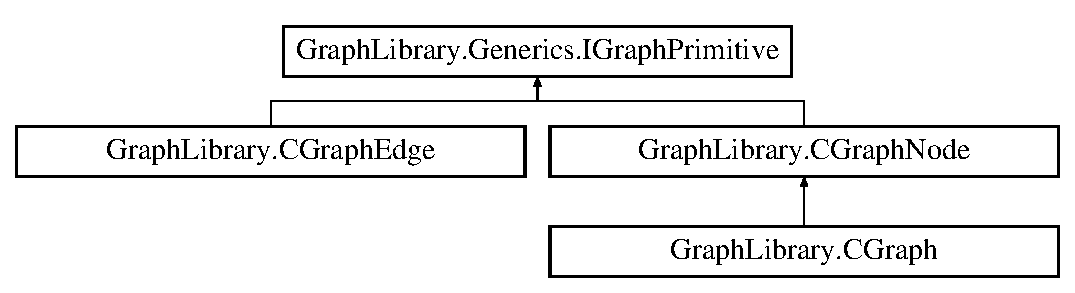
\includegraphics[height=3.000000cm]{interface_graph_library_1_1_generics_1_1_i_graph_primitive}
\end{center}
\end{figure}
\subsection*{Properties}
\begin{DoxyCompactItemize}
\item 
\hypertarget{interface_graph_library_1_1_generics_1_1_i_graph_primitive_a2d4ac2fb9b0322a490f620c18bd91eaa}{}int {\bfseries M\+\_\+\+Serial\+Number}\hspace{0.3cm}{\ttfamily  \mbox{[}get\mbox{]}}\label{interface_graph_library_1_1_generics_1_1_i_graph_primitive_a2d4ac2fb9b0322a490f620c18bd91eaa}

\item 
\hypertarget{interface_graph_library_1_1_generics_1_1_i_graph_primitive_a36eba4009bc50f09849dce0ea3657f7f}{}\hyperlink{namespace_graph_library_1_1_generics_a919a165f16deccdd1b3d7e8a93423fbc}{Graph\+Element\+Type} {\bfseries M\+\_\+\+Element\+Type}\hspace{0.3cm}{\ttfamily  \mbox{[}get\mbox{]}}\label{interface_graph_library_1_1_generics_1_1_i_graph_primitive_a36eba4009bc50f09849dce0ea3657f7f}

\end{DoxyCompactItemize}


\subsection{Detailed Description}
This interface contains primitive operations common to any graph element ( node, edge, graph ) 



The documentation for this interface was generated from the following file\+:\begin{DoxyCompactItemize}
\item 
Graph\+Library/\+Generics/Abstract\+Graph\+Elements.\+cs\end{DoxyCompactItemize}

\hypertarget{class_graph_library_1_1_c_it___graph_b_f_s_1_1_info___d_f_s}{}\section{Graph\+Library.\+C\+It\+\_\+\+Graph\+B\+F\+S.\+Info\+\_\+\+D\+F\+S Class Reference}
\label{class_graph_library_1_1_c_it___graph_b_f_s_1_1_info___d_f_s}\index{Graph\+Library.\+C\+It\+\_\+\+Graph\+B\+F\+S.\+Info\+\_\+\+D\+F\+S@{Graph\+Library.\+C\+It\+\_\+\+Graph\+B\+F\+S.\+Info\+\_\+\+D\+F\+S}}


Graph node info to assist the iterator algorithm  


\subsection*{Public Member Functions}
\begin{DoxyCompactItemize}
\item 
\hypertarget{class_graph_library_1_1_c_it___graph_b_f_s_1_1_info___d_f_s_a5ea2f57738f60298d90c9f2c74e5d862}{}{\bfseries Info\+\_\+\+D\+F\+S} (int m\+Color, int m\+Distance)\label{class_graph_library_1_1_c_it___graph_b_f_s_1_1_info___d_f_s_a5ea2f57738f60298d90c9f2c74e5d862}

\end{DoxyCompactItemize}
\subsection*{Public Attributes}
\begin{DoxyCompactItemize}
\item 
\hypertarget{class_graph_library_1_1_c_it___graph_b_f_s_1_1_info___d_f_s_a305bf8d7f018e0ab9f75d5873f42d098}{}int {\bfseries m\+\_\+color}\label{class_graph_library_1_1_c_it___graph_b_f_s_1_1_info___d_f_s_a305bf8d7f018e0ab9f75d5873f42d098}

\item 
\hypertarget{class_graph_library_1_1_c_it___graph_b_f_s_1_1_info___d_f_s_a331eb1a07629309df29d453109d55d03}{}int {\bfseries m\+\_\+distance}\label{class_graph_library_1_1_c_it___graph_b_f_s_1_1_info___d_f_s_a331eb1a07629309df29d453109d55d03}

\end{DoxyCompactItemize}


\subsection{Detailed Description}
Graph node info to assist the iterator algorithm 



The documentation for this class was generated from the following file\+:\begin{DoxyCompactItemize}
\item 
Graph\+Library/Graph\+Iterators.\+cs\end{DoxyCompactItemize}

\hypertarget{class_graph_library_1_1_c_it___graph_d_f_s_1_1_info___d_f_s}{}\section{Graph\+Library.\+C\+It\+\_\+\+Graph\+D\+F\+S.\+Info\+\_\+\+D\+F\+S Class Reference}
\label{class_graph_library_1_1_c_it___graph_d_f_s_1_1_info___d_f_s}\index{Graph\+Library.\+C\+It\+\_\+\+Graph\+D\+F\+S.\+Info\+\_\+\+D\+F\+S@{Graph\+Library.\+C\+It\+\_\+\+Graph\+D\+F\+S.\+Info\+\_\+\+D\+F\+S}}


Graph node info to assist the iterator algorithm  


\subsection*{Public Member Functions}
\begin{DoxyCompactItemize}
\item 
\hypertarget{class_graph_library_1_1_c_it___graph_d_f_s_1_1_info___d_f_s_ad028855e94bd2879809038ddf744120c}{}{\bfseries Info\+\_\+\+D\+F\+S} (int color)\label{class_graph_library_1_1_c_it___graph_d_f_s_1_1_info___d_f_s_ad028855e94bd2879809038ddf744120c}

\end{DoxyCompactItemize}
\subsection*{Public Attributes}
\begin{DoxyCompactItemize}
\item 
\hypertarget{class_graph_library_1_1_c_it___graph_d_f_s_1_1_info___d_f_s_a6107e582274d18723815dd6b9242c5af}{}int {\bfseries m\+\_\+color}\label{class_graph_library_1_1_c_it___graph_d_f_s_1_1_info___d_f_s_a6107e582274d18723815dd6b9242c5af}

\end{DoxyCompactItemize}


\subsection{Detailed Description}
Graph node info to assist the iterator algorithm 



The documentation for this class was generated from the following file\+:\begin{DoxyCompactItemize}
\item 
Graph\+Library/Graph\+Iterators.\+cs\end{DoxyCompactItemize}

\hypertarget{class_graph_library_1_1_aglorithms_1_1_node_info___d_f_s}{}\section{Graph\+Library.\+Aglorithms.\+Node\+Info\+\_\+\+D\+F\+S Class Reference}
\label{class_graph_library_1_1_aglorithms_1_1_node_info___d_f_s}\index{Graph\+Library.\+Aglorithms.\+Node\+Info\+\_\+\+D\+F\+S@{Graph\+Library.\+Aglorithms.\+Node\+Info\+\_\+\+D\+F\+S}}


Graph node info to assist the algorithm. Only the algorithm has access to the type of the Info\+\_\+\+D\+F\+S class. There could be also puclic Info class if the information is shared between diffrent algorithms. There is an instance of the Info\+\_\+\+D\+F\+S class in each graph node  


Inheritance diagram for Graph\+Library.\+Aglorithms.\+Node\+Info\+\_\+\+D\+F\+S\+:\begin{figure}[H]
\begin{center}
\leavevmode
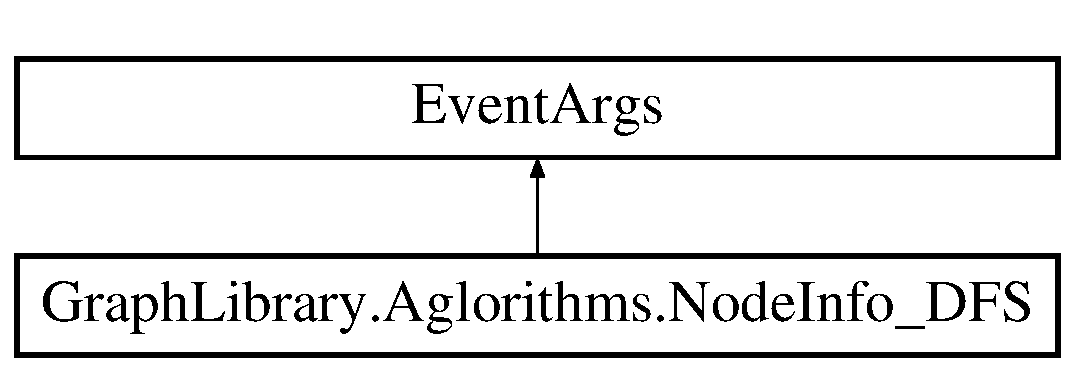
\includegraphics[height=2.000000cm]{class_graph_library_1_1_aglorithms_1_1_node_info___d_f_s}
\end{center}
\end{figure}
\subsection*{Public Member Functions}
\begin{DoxyCompactItemize}
\item 
\hypertarget{class_graph_library_1_1_aglorithms_1_1_node_info___d_f_s_ae88c8f29f110f22b7bbd4d6c7112a5ef}{}{\bfseries Node\+Info\+\_\+\+D\+F\+S} (int color)\label{class_graph_library_1_1_aglorithms_1_1_node_info___d_f_s_ae88c8f29f110f22b7bbd4d6c7112a5ef}

\end{DoxyCompactItemize}
\subsection*{Public Attributes}
\begin{DoxyCompactItemize}
\item 
\hypertarget{class_graph_library_1_1_aglorithms_1_1_node_info___d_f_s_a9e2567b2a65afa785c3ed74e2d80d9e5}{}int {\bfseries m\+\_\+color}\label{class_graph_library_1_1_aglorithms_1_1_node_info___d_f_s_a9e2567b2a65afa785c3ed74e2d80d9e5}

\end{DoxyCompactItemize}


\subsection{Detailed Description}
Graph node info to assist the algorithm. Only the algorithm has access to the type of the Info\+\_\+\+D\+F\+S class. There could be also puclic Info class if the information is shared between diffrent algorithms. There is an instance of the Info\+\_\+\+D\+F\+S class in each graph node 



The documentation for this class was generated from the following file\+:\begin{DoxyCompactItemize}
\item 
Graph\+Library/\+Aglorithms/Info\+\_\+\+D\+F\+S.\+cs\end{DoxyCompactItemize}

%--- End generated contents ---

% Index
\backmatter
\newpage
\phantomsection
\clearemptydoublepage
\addcontentsline{toc}{chapter}{Index}
\printindex

\end{document}
